% -*- Mode:TeX -*-

%% IMPORTANT: The official thesis specifications are available at:
%%            http://libraries.mit.edu/archives/thesis-specs/
%%
%%            Please verify your thesis' formatting and copyright
%%            assignment before submission.  If you notice any
%%            discrepancies between these templates and the 
%%            MIT Libraries' specs, please let us know
%%            by e-mailing thesis@mit.edu

%% The documentclass options along with the pagestyle can be used to generate
%% a technical report, a draft copy, or a regular thesis.  You may need to
%% re-specify the pagestyle after you \include  cover.tex.  For more
%% information, see the first few lines of mitthesis.cls. 

%\documentclass[12pt,vi,twoside]{mitthesis}
%%
%%  If you want your thesis copyright to you instead of MIT, use the
%%  ``vi'' option, as above.
%%
%\documentclass[12pt,twoside,leftblank]{mitthesis}
%%
%% If you want blank pages before new chapters to be labelled ``This
%% Page Intentionally Left Blank'', use the ``leftblank'' option, as
%% above. 

\documentclass[12pt,viii,twoside]{mitthesis}
\usepackage{lgrind}
%% These have been added at the request of the MIT Libraries, because
%% some PDF conversions mess up the ligatures.  -LB, 1/22/2014
\usepackage{cmap}
\usepackage[T1]{fontenc}
\usepackage{graphicx}
\usepackage{amsmath}
\usepackage{xspace}
\pagestyle{plain}

%% This bit allows you to either specify only the files which you wish to
%% process, or `all' to process all files which you \include.
%% Krishna Sethuraman (1990).

%% \typein [\files]{Enter file names to process, (chap1,chap2 ...), or `all' to
%% process all files:}
%% \def\all{all}
%% \ifx\files\all \typeout{Including all files.} \else \typeout{Including only \files.} \includeonly{\files} \fi

%% aliases
%% CMS Standard
\newcommand{\de}{\ensuremath{^\circ}}
\newcommand{\ten}[1]{\ensuremath{\times \text{10}^\text{#1}}}
\newcommand{\unit}[1]{\ensuremath{\text{\,#1}}\xspace}
\newcommand{\mum}{\ensuremath{\,\mu\text{m}}\xspace}
\newcommand{\micron}{\ensuremath{\,\mu\text{m}}\xspace}
\newcommand{\cm}{\ensuremath{\,\text{cm}}\xspace}
\newcommand{\mm}{\ensuremath{\,\text{mm}}\xspace}
\newcommand{\mus}{\ensuremath{\,\mu\text{s}}\xspace}
\newcommand{\keV}{\ensuremath{\,\text{ke\hspace{-.08em}V}}\xspace}
\newcommand{\MeV}{\ensuremath{\,\text{Me\hspace{-.08em}V}}\xspace}
\newcommand{\MeVns}{\ensuremath{\text{Me\hspace{-.08em}V}}\xspace} % no leading thinspace
\newcommand{\GeV}{\ensuremath{\,\text{Ge\hspace{-.08em}V}}\xspace}
\newcommand{\GeVns}{\ensuremath{\text{Ge\hspace{-.08em}V}}\xspace} % no leading thinspace
\newcommand{\gev}{\GeV}
\newcommand{\TeV}{\ensuremath{\,\text{Te\hspace{-.08em}V}}\xspace}
\newcommand{\TeVns}{\ensuremath{\text{Te\hspace{-.08em}V}}\xspace} % no leading thinspace
\newcommand{\PeV}{\ensuremath{\,\text{Pe\hspace{-.08em}V}}\xspace}
\newcommand{\keVc}{\ensuremath{{\,\text{ke\hspace{-.08em}V\hspace{-0.16em}/\hspace{-0.08em}}c}}\xspace}
\newcommand{\MeVc}{\ensuremath{{\,\text{Me\hspace{-.08em}V\hspace{-0.16em}/\hspace{-0.08em}}c}}\xspace}
\newcommand{\GeVc}{\ensuremath{{\,\text{Ge\hspace{-.08em}V\hspace{-0.16em}/\hspace{-0.08em}}c}}\xspace}
\newcommand{\GeVcns}{\ensuremath{{\text{Ge\hspace{-.08em}V\hspace{-0.16em}/\hspace{-0.08em}}c}}\xspace} % no leading thinspace
\newcommand{\TeVc}{\ensuremath{{\,\text{Te\hspace{-.08em}V\hspace{-0.16em}/\hspace{-0.08em}}c}}\xspace}
\newcommand{\keVcc}{\ensuremath{{\,\text{ke\hspace{-.08em}V\hspace{-0.16em}/\hspace{-0.08em}}c^\text{2}}}\xspace}
\newcommand{\MeVcc}{\ensuremath{{\,\text{Me\hspace{-.08em}V\hspace{-0.16em}/\hspace{-0.08em}}c^\text{2}}}\xspace}
\newcommand{\GeVcc}{\ensuremath{{\,\text{Ge\hspace{-.08em}V\hspace{-0.16em}/\hspace{-0.08em}}c^\text{2}}}\xspace}
\newcommand{\GeVccns}{\ensuremath{{\text{Ge\hspace{-.08em}V\hspace{-0.16em}/\hspace{-0.08em}}c^\text{2}}}\xspace} % no leading thinspace
\newcommand{\TeVcc}{\ensuremath{{\,\text{Te\hspace{-.08em}V\hspace{-0.16em}/\hspace{-0.08em}}c^\text{2}}}\xspace}

\newcommand{\abinv} {\mbox{\ensuremath{\,\text{ab}^{-1}}}\xspace}
\newcommand{\fbinv} {\mbox{\ensuremath{\,\text{fb}^{-1}}}\xspace}
\newcommand{\pbinv} {\mbox{\ensuremath{\,\text{pb}^{-1}}}\xspace}
\newcommand{\nbinv} {\mbox{\ensuremath{\,\text{nb}^{-1}}}\xspace}
\newcommand{\mubinv} {\ensuremath{\,\mu\text{b}^{-1}}\xspace}
\newcommand{\mbinv} {\ensuremath{\,\text{mb}^{-1}}\xspace}
\newcommand{\percms}{\ensuremath{\,\text{cm}^{-2}\,\text{s}^{-1}}\xspace}
\newcommand{\lumi}{\ensuremath{\mathcal{L}}\xspace}
\newcommand{\Lumi}{\ensuremath{\mathcal{L}}\xspace}%both upper and lower

\newcommand{\pt}{\ensuremath{p_{\mathrm{T}}}\xspace}
\newcommand{\et}{\ensuremath{E_{\mathrm{T}}}\xspace}
\newcommand{\mT}{\ensuremath{m_{\mathrm{T}}}\xspace}
\newcommand{\HT}{\ensuremath{H_{\mathrm{T}}}\xspace}
\newcommand{\ETm}{\ensuremath{E_{\mathrm{T}}^{\text{miss}}}\xspace}
\newcommand{\ptmiss}{\ensuremath{\pt^\text{miss}}\xspace}
\newcommand{\ptvec}{\ensuremath{{\vec p}_{\mathrm{T}}}\xspace}
\newcommand{\ptvecmiss}{\ensuremath{{\vec p}_{\mathrm{T}}^{\kern1pt\text{miss}}}\xspace}

\newcommand{\ttbar}{\ensuremath{{t}\overline{{t}}}\xspace} 
\newcommand{\Pgg}{\ensuremath{\gamma}\xspace}
\newcommand{\PZ}{\ensuremath{{Z}}\xspace}
\newcommand{\PW}{\ensuremath{{W}}\xspace}
\newcommand{\Pe}{\ensuremath{{e}}\xspace}
\newcommand{\Pgm}{\ensuremath{{\mu}}\xspace}
\newcommand{\PGn}{\ensuremath{\nu}\xspace}
\newcommand{\PAGn}{\ensuremath{\overline{\nu}}\xspace}
\newcommand{\Pq}{\ensuremath{{q}}\xspace}


%% from EXO-16-053
\newcommand{\nhalo}[1][]{\ensuremath{n^{\text{halo}}_{K#1}}}
\newcommand{\NZg}[1][]{\ensuremath{N^{\PZ\Pgg}_{#1}}}
\newcommand{\NWg}[1][]{\ensuremath{N^{\PW\Pgg}_{#1}}}
\newcommand{\RZll}[1][]{\ensuremath{R^{\PZ\Pgg}_{\ell\ell\Pgg#1}}}
\newcommand{\RZee}[1][]{\ensuremath{R^{\PZ\Pgg}_{\Pe\Pe\Pgg#1}}}
\newcommand{\RZmm}[1][]{\ensuremath{R^{\PZ\Pgg}_{\Pgm\Pgm\Pgg#1}}}
\newcommand{\RWl}[1][]{\ensuremath{R^{\PW\Pgg}_{\ell\Pgg#1}}}
\newcommand{\RWe}[1][]{\ensuremath{R^{\PW\Pgg}_{\Pe\Pgg#1}}}
\newcommand{\RWm}[1][]{\ensuremath{R^{\PW\Pgg}_{\Pgm\Pgg#1}}}
\newcommand{\fZW}[1][]{\ensuremath{f^{\PZ\Pgg}_{\PW\Pgg#1}}}
\newcommand{\Tll}[1][]{\ensuremath{T_{\ell\ell\Pgg#1}}}
\newcommand{\Tl}[1][]{\ensuremath{T_{\ell\Pgg#1}}}
\newcommand{\TK}[1][]{\ensuremath{T_{K#1}}}

\newcommand{\ETg}{\ensuremath{E_{\mathrm{T}}^{\Pgg}}\xspace}

\newcommand{\zinvg}{\ensuremath{\PZ(\to\PGn\PAGn){+}\Pgg}}
\newcommand{\zllg}{\ensuremath{\PZ(\to\ell\overline{\ell}){+}\Pgg}}
\newcommand{\wlng}{\ensuremath{\PW(\to\ell\PGn){+}\Pgg}}
\newcommand{\vg}{\ensuremath{\mathrm{V}{+}\Pgg}}
\newcommand{\gj}{\ensuremath{\Pgg{+}\text{jets}}}
\newcommand{\ttg}{\ensuremath{\ttbar\Pgg}\xspace}

\newcommand{\mdm}{\ensuremath{m_{\text{DM}}}}
\newcommand{\mmed}{\ensuremath{M_{\text{med}}}}
\newcommand{\gDM}{\ensuremath{\text{\usefont{OT1}{cmr}{m}{it}g}_{\text{DM}}}}
\newcommand{\gq}{\ensuremath{\text{\usefont{OT1}{cmr}{m}{it}g}_{\Pq}}}

\newcommand{\CL}{CL\xspace}

\begin{document}

% -*-latex-*-
% 
% For questions, comments, concerns or complaints:
% thesis@mit.edu
% 
%
% $Log: cover.tex,v $
% Revision 1.8  2008/05/13 15:02:15  jdreed
% Degree month is June, not May.  Added note about prevdegrees.
% Arthur Smith's title updated
%
% Revision 1.7  2001/02/08 18:53:16  boojum
% changed some \newpages to \cleardoublepages
%
% Revision 1.6  1999/10/21 14:49:31  boojum
% changed comment referring to documentstyle
%
% Revision 1.5  1999/10/21 14:39:04  boojum
% *** empty log message ***
%
% Revision 1.4  1997/04/18  17:54:10  othomas
% added page numbers on abstract and cover, and made 1 abstract
% page the default rather than 2.  (anne hunter tells me this
% is the new institute standard.)
%
% Revision 1.4  1997/04/18  17:54:10  othomas
% added page numbers on abstract and cover, and made 1 abstract
% page the default rather than 2.  (anne hunter tells me this
% is the new institute standard.)
%
% Revision 1.3  93/05/17  17:06:29  starflt
% Added acknowledgements section (suggested by tompalka)
% 
% Revision 1.2  92/04/22  13:13:13  epeisach
% Fixes for 1991 course 6 requirements
% Phrase "and to grant others the right to do so" has been added to 
% permission clause
% Second copy of abstract is not counted as separate pages so numbering works
% out
% 
% Revision 1.1  92/04/22  13:08:20  epeisach

% NOTE:
% These templates make an effort to conform to the MIT Thesis specifications,
% however the specifications can change.  We recommend that you verify the
% layout of your title page with your thesis advisor and/or the MIT 
% Libraries before printing your final copy.
% \title{Shining Light on Dark Matter, \\ One Photon at a Time}
\title{Searching for Dark Matter with the CMS Detector \\in proton-proton collisions containing \\a single high-\pt\ photon and large \met\ }
  
\author{Brandon Leigh Allen}
% If you wish to list your previous degrees on the cover page, use the 
% previous degrees command:
%       \prevdegrees{A.A., Harvard University (1985)}
% You can use the \\ command to list multiple previous degrees
%       \prevdegrees{B.S., University of California (1978) \\
%                    S.M., Massachusetts Institute of Technology (1981)}
\department{Department of Physics}

% If the thesis is for two degrees simultaneously, list them both
% separated by \and like this:
% \degree{Doctor of Philosophy \and Master of Science}
\degree{Doctorate of Philosophy in Physics}

% As of the 2007-08 academic year, valid degree months are September, 
% February, or June.  The default is June.
\degreemonth{June}
\degreeyear{2019}
\thesisdate{May 18, 2019}

%% By default, the thesis will be copyrighted to MIT.  If you need to copyright
%% the thesis to yourself, just specify the `vi' documentclass option.  If for
%% some reason you want to exactly specify the copyright notice text, you can
%% use the \copyrightnoticetext command.  
%\copyrightnoticetext{\copyright IBM, 1990.  Do not open till Xmas.}

% If there is more than one supervisor, use the \supervisor command
% once for each.
\supervisor{Christoph E.M. Paus}{Professor}

% This is the department committee chairman, not the thesis committee
% chairman.  You should replace this with your Department's Committee
% Chairman.
\chairman{Nergis Mavalvala}{Associate Department Head for Education}

% Make the titlepage based on the above information.  If you need
% something special and can't use the standard form, you can specify
% the exact text of the titlepage yourself.  Put it in a titlepage
% environment and leave blank lines where you want vertical space.
% The spaces will be adjusted to fill the entire page.  The dotted
% lines for the signatures are made with the \signature command.
\maketitle

% The abstractpage environment sets up everything on the page except
% the text itself.  The title and other header material are put at the
% top of the page, and the supervisors are listed at the bottom.  A
% new page is begun both before and after.  Of course, an abstract may
% be more than one page itself.  If you need more control over the
% format of the page, you can use the abstract environment, which puts
% the word "Abstract" at the beginning and single spaces its text.

%% You can either \input (*not* \include) your abstract file, or you can put
%% the text of the abstract directly between the \begin{abstractpage} and
%% \end{abstractpage} commands.

% First copy: start a new page, and save the page number.
\cleardoublepage
% Uncomment the next line if you do NOT want a page number on your
% abstract and acknowledgments pages.
% \pagestyle{empty}
\setcounter{savepage}{\thepage}
\begin{abstractpage}
% $Log: abstract.tex,v $
% Revision 1.1  93/05/14  14:56:25  starflt
% Initial revision
% 
% Revision 1.1  90/05/04  10:41:01  lwvanels
% Initial revision
% 
%
%% The text of your abstract and nothing else (other than comments) goes here.
%% It will be single-spaced and the rest of the text that is supposed to go on
%% the abstract page will be generated by the abstractpage environment.  This
%% file should be \input (not \include 'd) from cover.tex.
A search is conducted for new physics in final states containing a photon and missing transverse momentum in proton-proton collisions at $\sqrt{s} = 13$ TeV.
The data collected by the CMS experiment at the CERN LHC correspond to an integrated luminosity of 35.9 inverse femtobarns.
No deviations from the predictions of the standard model are observed. 
The results are interpreted in the context of dark matter production and limits on new physics parameters are calculated at 95\% confidence level. 
For the two simplified dark matter production models considered, the observed (expected) lower limits on the mediator masses are both 950\,(1150)\GeV for 1\GeV dark matter mass.

\end{abstractpage}

% Additional copy: start a new page, and reset the page number.  This way,
% the second copy of the abstract is not counted as separate pages.
% Uncomment the next 6 lines if you need two copies of the abstract
% page.
% \setcounter{page}{\thesavepage}
% \begin{abstractpage}
% % $Log: abstract.tex,v $
% Revision 1.1  93/05/14  14:56:25  starflt
% Initial revision
% 
% Revision 1.1  90/05/04  10:41:01  lwvanels
% Initial revision
% 
%
%% The text of your abstract and nothing else (other than comments) goes here.
%% It will be single-spaced and the rest of the text that is supposed to go on
%% the abstract page will be generated by the abstractpage environment.  This
%% file should be \input (not \include 'd) from cover.tex.
A search is conducted for new physics in final states containing a photon and missing transverse momentum in proton-proton collisions at $\sqrt{s} = 13$ TeV.
The data collected by the CMS experiment at the CERN LHC correspond to an integrated luminosity of 35.9 inverse femtobarns.
No deviations from the predictions of the standard model are observed. 
The results are interpreted in the context of dark matter production and limits on new physics parameters are calculated at 95\% confidence level. 
For the two simplified dark matter production models considered, the observed (expected) lower limits on the mediator masses are both 950\,(1150)\GeV for 1\GeV dark matter mass.

% \end{abstractpage}

\cleardoublepage

\section*{Acknowledgments}

This is the acknowledgements section.  You should replace this with your
own acknowledgements.

%%%%%%%%%%%%%%%%%%%%%%%%%%%%%%%%%%%%%%%%%%%%%%%%%%%%%%%%%%%%%%%%%%%%%%
% -*-latex-*-

% Some departments (e.g. 5) require an additional signature page.  See
% signature.tex for more information and uncomment the following line if
% applicable.
% % -*- Mode:TeX -*-
%
% Some departments (e.g. Chemistry) require an additional cover page
% with signatures of the thesis committee.  Please check with your
% thesis advisor or other appropriate person to determine if such a 
% page is required for your thesis.  
%
% If you choose not to use the "titlepage" environment, a \newpage
% commands, and several \vspace{\fill} commands may be necessary to
% achieve the required spacing.  The \signature command is defined in
% the "mitthesis" class
%
% The following sample appears courtesy of Ben Kaduk <kaduk@mit.edu> and
% was used in his June 2012 doctoral thesis in Chemistry. 

\begin{titlepage}
\begin{large}
This doctoral thesis has been examined by a Committee of the Department
of Chemistry as follows:

\signature{Professor Jianshu Cao}{Chairman, Thesis Committee \\
   Professor of Chemistry}

\signature{Professor Troy Van Voorhis}{Thesis Supervisor \\
   Associate Professor of Chemistry}

\signature{Professor Robert W. Field}{Member, Thesis Committee \\
   Haslam and Dewey Professor of Chemistry}
\end{large}
\end{titlepage}


\pagestyle{plain}
  % -*- Mode:TeX -*-
%% This file simply contains the commands that actually generate the table of
%% contents and lists of figures and tables.  You can omit any or all of
%% these files by simply taking out the appropriate command.  For more
%% information on these files, see appendix C.3.3 of the LaTeX manual. 
\tableofcontents
\newpage
% \listoffigures
\newpage
% \listoftables


% \chapter{Introduction}

The Standard Model of particle physics was fully experimentally verified in 2012 with the discovery of the Higgs boson by the CMS and ATLAS collaborations at the Large Hadron Collider~\cite{HiggsPaper}.
The Standard Model completely explains all of our observations of the microscopic wold but fails at the scale of the universe, specifically with regards to gravitational interactions.
Many astrophysical observations of gravitational interactions provide strong evidence for the existence of dark matter, potentially explained by a new elementary particle not included in the Standard Model.
Many experiments test the hypothesis that dark matter has a such particle physics origin including searches for the direct production of dark matter at particle colliders.

In this thesis, we focus on a recent search for dark matter in proton-proton collisions resulting in a single high-\pt\ photon and large missing transverse momentum~\cite{Monophoton}.
First, we review the details of the Standard Model and the astrophysical evidence for dark matter.
Then, we describe the Large Hadron Collider, the Compact Muon Solenoid detector, and the methods used to reconstruct the data from the collisions.
Finally, we describe the analysis in detail and summarize the outlook for the future.

% \chapter{Motivation}

% Why I did this.

\section{The Standard Model}
\label{sec:sm}

The Standard Model (SM) of particle physics describes the physical properties and dynamics of fermions, the fundamental constituents of matter, and their interactions in the language of a Lorentz-invariant quantum field theory (QFT).
The Standard Model consists of a set of fermion fields, shown in Table~\ref{tab:fermions} and the local gauge symmetry group that acts on them
\begin{equation}
  G_{\text{SM}} = \suthree \times \sutwo \times \uone,
\end{equation}
which is composed of the subgroups
\begin{align}
  G_{\text{QCD}} & = \suthree \qquad \text{and} \nonumber \\
  G_{\text{EWK}} & = \sutwo \times \uone,
\end{align}
corresponding to the strong and electroweak interactions, respectively.
Each fermion field exists in a unique representation of $G_{\text{SM}}$, also summarized in Table~\ref{tab:fermions}.
The possible represenations of \suthree\ are triplet, conjugate, and singlet, denoted by $\mathbf{3}$, $\mathbf{\bar{3}}$, and $\mathbf{1}$, respectively, while the possible representations of \sutwo\ are doublet and singlet, denoted by $\mathbf{2}$ and $\mathbf{1}$, respectively.
All fermions exist in the singlet representation of \uone, only distinguished by differing values of the weak hypercharge $Y$.
Conversely, all fermions in non-singlet representations of \suthree\ and \sutwo\ have the same interaction strength, a feature known as universality.

\begin{table}[htbp]
\centering
\caption{
  The categories of SM fermions and the action of the SM local gauge symmetry group $G_{\text{SM}}$.
  Each category contains three members, one for each generation of the Standard Model.
  A corresponding table exists for the charge conjugated fields representing the anti-fermions.
  The subscripts $L$ and $R$ denote whether the field is left- or right-handed.
}
\label{tab:fermions}
\begin{tabular}{ l|c|c|c|c }
  Name & Symbol & $Y$ & \sutwo\ rep. & \suthree\ rep. \\
  \hline
  \hline
  Left-handed quark & $q_L$ & $\sfrac{1}{6}$ & \textbf{2} & \textbf{3} \\
  Right-handed up-type quark & $u_R$ & $\sfrac{2}{3}$ & \textbf{1} & \textbf{3} \\
  Right-handed down-type quark & $d_R$ & $\sfrac{-1}{3}$ & \textbf{1} & \textbf{3} \\
  \hline
  Left-handed lepton & $\ell_L$ & $\sfrac{-1}{2}$ & \textbf{2} & \textbf{1} \\
  Right-handed charged lepton & $e_R$ & -1 & \textbf{1} & \textbf{1} \\
  Right-handed neutrino & $\nu_R$ & $\sfrac{1}{6}$ & \textbf{1} & \textbf{1} \\
\end{tabular}
\end{table}

For each category of fermion listed in Table~\ref{tab:fermions}, there exist three generations or copies in the Standard Model, identical except for differing masses.
The lepton electroweak doublets contain the left-handed charged leptons and neutrinos
\begin{equation}
  \ell_{L} = \begin{pmatrix} \nu_e \\ e^-_L \end{pmatrix} ,
              \begin{pmatrix} \nu_\mu \\ \mu^-_L \end{pmatrix} ,
              \begin{pmatrix} \nu_\tau \\ \tau^-_L \end{pmatrix} ,
\end{equation}
and the right-handed lepton singlets contain the right-handed projections of the same leptons and neutrinos.
The quark electroweak doublets contain the left-handed up-type and down-type quarks
\begin{equation}
  q_{L} = \begin{pmatrix} u_L \\ d_L \end{pmatrix} ,
           \begin{pmatrix} c_L \\ s_L \end{pmatrix} ,
           \begin{pmatrix} t_L \\ b_L \end{pmatrix} ,
\end{equation}
and the right-handed quark singlets contain the right-handed projections of the same quarks.
% where $d'$, $s'$, and $b'$ are the electroweak eigenstates of the down-type quarks (further explained in Section~\ref{subsec:ewk}).
Quarks also exist in a strong triplet, which will be denoted with a superscript $c$ as necessary.

\subsection{Strong Interactions}
\label{subsec:qcd}

The strong interactions of quarks and gluons are described by quantum chromodynamics (QCD), with the Lagrangian
\begin{equation}
  \label{eqn:lqcd}
  \mathcal{L}_{\text{QCD}} = i \bar q_f^a \slashed D^{ab} q_f^b + m_f \bar q_f^a q_f^a - \frac{1}{4} G_{\mu\nu}^a G^{a,\mu\nu} + \theta \frac{g_s^2}{72\pi^2} \epsilon_{\mu\nu\rho\sigma} G^{c,\mu\nu} G^{c, \rho\sigma},
\end{equation}
where repeated indices are contracted.
The $q_f^a$ are the quark-field Dirac spinors of flavor $f \in \{u,d,c,s,t,b\}$, color $a \in \{r,g,b\}$ (the basis element of the triplet representation), and mass $m_f$.
The first term in Equation~\ref{eqn:lqcd} contains the QCD covariant derivative
\begin{equation}
  D_{\mu}^{ab} = \delta^{ab} \partial_\mu - i g_s \sum_{c} t_c^{ab} G_{c,\mu},
\end{equation}
where $g_s$ is the strong interaction coupling strength, $t_c$ are the eight $3\times3$ Hermitian traceless matrices that serve as the generators of the triplet representation of \suthree, and $G_c$ are the corresponding eight gluon fields.
The third term in Equation~\ref{eqn:lqcd} contains the gluon field strength tensors
\begin{equation}
  G_{\mu\nu}^a = \partial_\mu G_\nu^a - \partial_\nu G_\mu^a - g_s f^{abc} G_\mu^b G_\nu^C,
\end{equation}
where $f^{abc}$ are the structure constants of \suthree.
The non-Abelian structure of the \suthree\ group allows for 3-gluon and 4-gluon interactions in addition to the quark-antiquark-gluon interactions.

The last term in Equation~\ref{eqn:lqcd} violates CP conservation and produces a non-zero electric dipole moment (EDM) for the neutron.
Experimental limits onthe neutron EDM constraint the QCD vaccum angle $\theta$ to be smaller than $10^{-10}$.
The Peccei-Quinn theory provides a possible method to force $\theta$ to zero by introducing the hypothetical axion particle. The axion is a potential dark matter candidate and will be discussed further in Section~\ref{sec:dm}.

\subsection{Hadrons}
\label{sec:hadrons}

Free quarks and gluons are not observed in nature, only in bound states called hadrons.
This is a consequence of two factors: color confinement and aysmptotic freedom.

Color confinement is the hypothesis that colored objects are always confined to color singlet states and that no objects with non-zero color charge can propagate as free particles.
Thus, quarks can only exist in bound states of a quark-antiquark pair or three quarks, called mesons and baryons, respectively. 
Since gluons carry a color charge, they are confined to hadrons as well.
Confinement is a low-energy non-pertubative phenomenon, occuring only below the QCD confinement scale \lqcd. 
An analytic proof of color confinement does not exist currently; however, the running of the strong coupling constant $\alpha_s = \sfrac{g_s^2}{4\pi}$ provides a mechanism for it.

Due to higher-order corrections to propagators in a QFT, physical quantities such as coupling constants and masses acquire a scale-dependence, where the value of the quantity changes as a function of the probed energy scale $q^2$.
The process of recovering scale-invariance is called renormalization and ensures that any divergent terms from the higher-order corrections cancel out in the physical values.
Given the value of an arbitrary coupling constant $\alpha$ at some known scale $\mu^2$, the value of $\alpha$ at arbitrary scale $q^2$ is  
\begin{equation}
  \label{eqn:rge}
  \alpha (q^2) = \frac{\alpha(\mu^2)}{1 - \alpha(\mu^2) \left[ \Pi(q^2) - \Pi(\mu^2) \right]},
\end{equation}
where $\Pi(q^2)$ and $\Pi(\mu^2)$ are the self-energy correction of the propagator at scales $q^2$ and $\mu^2$.
While these individual terms are separately divergent, their difference is finite and calculable. 

For values of $q^2$ and $\mu^2$ larger than the confinement scale \lqcd, the difference between the gluon self-energy corrections to one-loop order is given by 
\begin{equation}
  \label{eqn:beta_qcd}
  \Pi_s(q^2) - \Pi_s(\mu^2) \approx - \frac{\beta}{4\pi} \ln \left( \dfrac{q^2}{\mu^2} \right)
\end{equation}
where $\beta$ depends on the number of quark and gluon loops.
For $N_c$ colors and $N_f$ quark flavors with mass below $\abs q$,
\begin{equation}
  \beta = \frac{11 N_c - 2 N_f}{12 \pi}. 
\end{equation}
In the Standard Model, $N_c = 3$ and $N_f \le 6$ regardless of energy, thus $\beta$ is always positive.
Combining Equations~\ref{eqn:rge} and~\ref{eqn:beta_qcd}, the evolution of $\alpha_s$ is given by
\begin{equation}
  \label{eqn:alpha_s}
  \alpha_s (q^2) = \frac{\alpha_s(\mu^2)}{1 + \beta \alpha_s (\mu^2) \ln \left( \dfrac{q^2}{\mu^2} \right)} \approx \frac{1}{\beta \ln \left( \dfrac{q^2}{\lqcd^2} \right)}
\end{equation}
for a sufficiently large energy scale $q^2 \gg \lqcd^2$.
Through electron-positron collisions, the value of $\alpha_s$ at the $Z$-pole has been measured to be $\alpha_s (m_Z^2) = 0.1181 \pm 0.0011$ with a corresponding confinement scale of $\lqcd = 218\MeV$.  

From Equation~\ref{eqn:alpha_s}, we see that $\alpha_s$ decreases with increasing $q^2$.
At $\abs q \sim 1\GeV$, the value of $\alpha_s$ is of $\mathcal{O}(1)$ confining quarks and gluons to hadrons in a strongly-bound non-perturbative state.
However, $\abs q \gtrsim 100\GeV$, we have $\alpha_s \approx 0.1$ which is small eneough that perturbation theory can be used and quarks can be treated as quasi-free particles.
This property of QCD is known as asymptotic freedom.

%\newpage
\subsection{Electroweak Interactions}
\label{subsec:ewk}

The electroweak interactions of fermions are described by $\sutwo \times \uone$ gauge group, with the Lagrangian
\begin{equation}
  \label{eqn:lewk}
  \mathcal{L}_{\text{EWK}} = i \bar \psi_i \slashed D \psi_i - \frac{1}{4} \vec W_{\mu\nu} \cdot \vec W^{\mu\nu} - \frac{1}{4} B_{\mu\nu} B^{\mu\nu}
\end{equation}
where repeated indices are contracted and $\psi \supseteq \{q_L, u_R, d_R, \ell_L, e_R, \nu_R\}$ is the set of SM fermions, and the gauge field tensors are given by
\begin{align}
  B_{\mu\nu} & = \partial_\mu B_\nu - \partial_\nu B_\mu \qquad \text{and} \nonumber \\
  \vec W_{\mu\nu} & = \partial_\mu \vec W_\nu - \partial_\nu \vec W_\mu + g \vec W^\mu \times \vec W^\nu ,
\end{align}
where $\vec W_\mu$ and $B_\mu$ are the gauge fields for \sutwo\ and \uone, respectively, and $g$ is the coupling strength for \sutwo.
The first term in Equation~\ref{eqn:lewk} contains the EWK covariant derivative
\begin{equation}
  D_{\mu} = \partial_\mu - i g \vec T \cdot \vec W_\mu - i g' Y B_\mu,
\end{equation}
where $g'$ is the coupling strength for \uone,
$Y$ is the \uone\ hypercharge of the fermion field,
and $\vec T$ are the generators of the doublet representation of \sutwo.
The generators can be written in terms of the Pauli spin matrices $\vec T = \vec \sigma / 2$ and only have non-zero action on left-handed particles. %  and right-handed antiparticles.
% and $\delta_L$ is 1 if the fermion field is left-handed and 0 if it is right-handed.
The values of the hypercharge $Y$ shown in Table~\ref{tab:fermions} are chosen such that the physical electric charge of each fermion is given by $Q =  T_3 + Y$.

Notice that Equation~\ref{eqn:lewk} does not contain a Dirac mass term like that found in Equation~\ref{eqn:lqcd}.
This is because the term
\begin{equation}
  m \bar \psi \psi = m \left( \bar \psi_L \psi_R + \bar \psi_R \psi_L \right)
\end{equation}
mixes the left-handed and right-handed fermions leading to a Lagrangian that is no longer invariant under \sutwo.
As the observed fermions are not massless, the Lagrangian given in Equation~\ref{eqn:lewk} is incomplete and an additional mechanism needs to be introduced to produce non-zero fermion masses.

\subsection{Electroweak Symmetry Breaking}
\label{subsec:ewsb}

Spontaneous electroweak symmetry breaking provides the mechanism we need, as well as providing masses to the weak gauge bosons. The \sutwo\ symmetry is broken by introducing a left-handed complex scalar doublet $\phi$ with $Y_\phi = \sfrac{1}{2}$ to the Lagrangian in the following manner
\begin{equation}
  \label{eqn:ewsb}
  \mathcal{L}_{\text{EWK}} \mapsto \mathcal{L}_{\text{EWK}} + \left|D_\mu \phi \right|^2 + \mu^2 \phi^2 - \lambda \left| \phi \right|^4 .
\end{equation}
We choose to write this complex doublet, known as the complex Higgs field, in terms of four real-valued fields so that
\begin{equation}
  \phi = \frac{1}{\sqrt{2}} \begin{pmatrix} \phi_1 + i \phi_2 \\ \phi_3 + i\phi_4 \end{pmatrix} .
\end{equation}
Fortunately, the two self-interaction terms create a Higgs potential with a degenerate global minimum at the vacuum expectation value (vev)
\begin{equation}
  v \equiv \langle | \phi | \rangle = \sqrt{ \frac{\mu^2}{\lambda}},
\end{equation}
and through gauge rotations we set $\langle \phi_{1,2,4} \rangle = 0$, removing three degrees of freedom and producing three massless Nambu-Goldstone bosons.
The remaining degree of freedom is the real Higgs field $H$ which expresses small peturbations around the vev in the third component of the complex Higgs field $\phi_3 = v + H$.

The kinetic term in Equation~\ref{eqn:ewsb} couples the complex Higgs field to the EWK gauge bosons as follows at the vev
\begin{equation}
  \left| D_\mu \phi \right|^2 = \frac{v^2}{8} \left[ \left(g W_\mu^1 \right)^2 + \left(g W_\mu^2 \right)^2 + \left(g' B_\mu - g W_\mu^3 \right)^2 \right].
\end{equation}
%\newpage 
Diagonalizing this term gives rise to the three massive weak bosons and the massless photon that we observe in nature:
\begin{equation}
  \begin{matrix}[l | l]
    W_\mu^{\pm} \equiv \frac{1}{\sqrt{2}} \left( W_\mu^1 \mp W_\mu^2 \right)
    & m_W = \frac{1}{2} vg \\
    Z_\mu \equiv \cos \thetaw W_\mu^3 - \sin \thetaw B_\mu
    & m_Z = \frac{1}{2} v \sqrt{g^2 + (g')^2} \\
    A_\mu \equiv \sin \thetaw W_\mu^3 + \cos \thetaw B_\mu
    & m_A = 0,
  \end{matrix}
\end{equation}
where $\tan \thetaw = g'/g$.
With this, we rewrite Equation~\ref{eqn:lewk} in terms of the observed electromagnetic, charged weaked, and neutral weak currents as follows:
\begin{align}
  \label{eqn:lewsb}
  \mathcal{L}_{\text{EWK}} % &= \mathcal{L}_{\text{EM}} + \mathcal{L}_{\text{CC}} + \mathcal{L}_{\text{NC}} \nonumber \\
  = \bar \psi_i \left( i \slashed \partial - e Q \slashed A \right) \psi_i
  & - \frac{g}{2\sqrt{2}} \bar \psi_i \left( T^+ \slashed W^+ + T^- \slashed W^- \right) \psi_i - \frac{1}{2} m_W^2 W_\mu^+ W^{-\mu} \nonumber \\
   & - \frac{g}{2 \cos \thetaw} \bar \psi_i (g_V - g_A \gamma^5) \slashed Z \psi_i - \frac{1}{2} m_Z^2 Z_\mu Z^\mu, 
\end{align}
where $e = g' \cos \thetaw$ is the charge of the electron, $T^\pm = (T_1 \mp i T_2)/\sqrt{2}$ are the weak isospin raising and lowering operators, and $g_V = T_3$ and $g_A = T_3 - 2 Q \sin^2 \thetaw$ are the vector and axial-vector couplings for the neutral weak current.

We can also expand Equation~\ref{eqn:ewsb} about the vev giving us the following Higgs Lagrangian
\begin{align}
  \mathcal{L}_H = \frac{1}{2} \partial_\mu H \partial^\mu H - \frac{1}{2} m_H^2 H^2
  & + \frac{m_H^2}{2 v} H^3 + \frac{2 m_W^2}{v} W_\mu^+ W^{-\mu} H + \frac{m_Z^2}{v} Z_\mu Z^\mu H \nonumber \\
  & + \frac{m_H^2}{8 v^2} H^4 + \frac{m_W^2}{v^2} W_\mu^+ W^{-\mu} H^2 + \frac{m_Z^2}{2v^2} Z_\mu Z^\mu H^2, 
\end{align}
where $m_H = \mu \sqrt{2} $.
Thus, we see that the real Higgs field $H$ has trilinear and quartic couplings to itself and the weak gauge bosons with coupling strengths proportional to the mass squared of the appropriate boson.
This suggests a way to introduce fermion masses through the Higgs field.

%\newpage
\subsection{Fermion Masses}
\label{subsec:yukawa}

Introducing Yukawa couplings between the complex Higgs field $\phi$ and the SM fermion fields enables us to add mass terms for the fermions.
First, we start with the terms for charged leptons,
\begin{equation}
  \label{eqn:lyuk}
  \mathcal{L}^{\text{leptons}}_{\text{Y}} = - \bar \ell_L Y_e \phi e_R - \bar e_R Y_e \phi^\dagger \ell_L,
\end{equation}
where $Y_e$ is the Yukawa matrix for the charged leptons.
In general, Yukawa matrices and thus mass matrices are non-diagonal and hence we need to convert from the electroweak eigenstates $f_{L,R}$ to the mass eigenstates $\tilde{f}_{L,R} = U^{f}_{L,R} f_{L,R}$ where $U^{f}_{L,R}$ is a unitary matrix.
With this we rewrite Equation~\ref{eqn:lyuk} in terms of the mass eigenstates
\begin{align}
  \mathcal{L}^{\text{leptons}}_{\text{Y}} & = - \bar{\tilde{\ell}}_{L} U^e_L Y_e \phi U^{e\dagger}_R \tilde{e}_{R} - \bar{\tilde{e}}_{R} U^e_R Y_e \phi^\dagger U^{e\dagger}_L \tilde{\ell}_{L} \nonumber \\
  & = - \bar{\tilde{\ell}}_{L} \tilde Y_e \phi \tilde{e}_{R} - \bar{\tilde{e}}_{R} \tilde Y_e^\dagger \phi^\dagger \tilde{\ell}_{L}, 
\end{align}
where $\tilde Y_e = U^e_L Y_e U^{e\dagger}_R$ is the diagonalized Yukawa matrix for the charged leptons.
After electroweak symmetry breaking, these terms become
\begin{align}
  \mathcal{L}^{\text{leptons}}_{\text{Y}} & = - \frac{v + H}{\sqrt{2}} \left( \bar{\tilde{e}}_L \tilde Y_e  \tilde{e}_R + \bar{\tilde{e}}_R \tilde Y_e^\dagger \tilde{e}_L \right) \nonumber \\
  & = - \left(1 + \frac{H}{v}\right) \left( \bar{\tilde{e}}_L \tilde M_e \tilde{e}_R + \bar{\tilde{e}}_R \tilde M_e^\dagger \tilde{e}_L \right) \nonumber \\
  & = - \tilde M_e \bar e e - \frac{\tilde M_e}{v} \bar e e H,
    \label{eqn:lmass}
\end{align}
where $\tilde M_e = v \tilde Y_e / \sqrt{2}$ is the diagonalized mass matrix for the charged leptons and $e$ is the set of massive Dirac spinors for the charged leptons.

From Equation~\ref{eqn:lmass}, we see that the Yukawa couplings between the complex Higgs field $\phi$ and the charged leptons result in a Dirac mass term and a coupling to the real Higgs field $H$ that is proportional to the mass of the charged leptons and the vev.
The same procedure is used to introduce mass terms for the down-type quarks whereas for the neutrinos and up-type quarks we must use the conjugate doublet $\phi_c = - i \sigma_2 \phi^*$ in place of $\phi$ to obtain the same result.

\subsection{Flavor Mixing}

For the charged leptons and up-type quarks, it is possible to define a basis of simultaneous electroweak and mass eigenstates, so in practice $\tilde Y_{e,u} = Y_{e,u}$ as $U^{e,u}_L = U^{e,u}_R = \mathit{\mathbf{I}}$.
However, it is not possible to do this for the neutrinos at the same time as the charged leptons or for the down-type quarks at the same time as the up-type quarks.

In Equation~\ref{eqn:lewsb}, the charged current term involves interactions between the up-type and down-type quarks and is not preserved under the transform $f \rightarrow \tilde f$.
Writing this in terms of the mass eigenstates we have
\begin{align}
  \mathcal{L}_{\text{CC}} % & = - \frac{g}{2\sqrt{2}} \bar Q_L \left( T^+ \slashed W^+ + T^- \slashed W^- \right) Q_L \nonumber \\
  & = - \frac{g}{2\sqrt{2}} \left( \bar u_L T^+ \slashed W^+ d_L + \bar d_L T^- \slashed W^- u_L \right) \nonumber \\
  % & = - \frac{g}{2\sqrt{2}} \left( \bar{\tilde{u}}_L U^{u\dagger}_L T^+ \slashed W^+ U^d_L \tilde{d}_L + \bar{\tilde{d}}_L U^{d\dagger}_L T^- \slashed W^- U^u_L \tilde{u}_L \right) \nonumber \\
  & = - \frac{g}{2\sqrt{2}} \left( \bar{u}_L  T^+ \slashed W^+ \vckm \tilde{d}_L + \bar{\tilde{d}}_L T^- \slashed W^- \vckm^\dagger u_L \right),
\end{align}
where $\vckm = U^{u\dagger}_L U^d_L$ is the Cabibbo-Kaboyshi-Maskawa matrix and $u_L = \tilde{u}_L$ by construction.
The CKM matrix is unitary with four free parameters, the mixing angles between quark generations $\phi_{12} = 13.1$, $\phi_{23}$, and $\phi_{13}$ as well as a CP-violating phase $\delta$.
In terms of these parameters, the CKM matrix is
\begin{equation}
  \vckm = \begin{pmatrix} c_{12} & s_{12} & 0 \\ - s_{12} & c_{12} & 0 \\ 0 & 0 & 1 \end{pmatrix}
  \times \begin{pmatrix} 1 & 0 & 0  \\ 0 & c_{23} & s_{23} \\ 0 & - s_{23} & c_{23} \end{pmatrix}
  \times \begin{pmatrix} c_{13} & 0 & s_{13} e^{-i\delta} \\ 0 & 1 & 0 \\ -s_{13} e^{i\delta} & 0 & c_{13} \end{pmatrix},
\end{equation}
where $s_{ij} = \sin \phi_{ij}$ and $c_{ij} = \cos \phi_{ij}$.
It has been experimentally determined that the CKM is mostly diagonal with $s_{13} \ll s_{23} \ll s_{12} \ll 1$. 

The equivalent mixing matrix for the neutrinos is the Pontecorvo-Maki-Nakagawa-Sakata matrix \upmns, which  converts from the mass eigenstates $\nu_1$, $\nu_2$, and $\nu_3$ to the electroweak eigenstates $\nu_e$, $\nu_\mu$, $\nu_\tau$.
Unlike the CKM matrix, the PMNS is non-diagonal resulting in stronger mixing in the neutrino sector.
The values of the mixing angles $\theta_{12}$, $\theta_{23}$, and $\theta_{13}$ have been measured in neutrino oscillation experiments while the CP-violating phase $\delta'$ has not yet been directly measured.
From cosmological measurements, % of the large-scale structure of the universe,
it is known that the sum of the neutrino masses is less than one eV. 

% \newpage
\subsection{Summary}

\begin{table}[htbp]
\centering
\caption{ The free parameters of the Standard Model, not including masses.}
\label{tab:sm_params}
\begin{tabular}{ c|l|r }
  Parameter & Description & Best Fit Value \\
  \hline
  \hline
  $\phi_{12}$ & CKM 12-mixing anlge    & $13.1^\circ$ \\
  $\phi_{23}$ & CKM 23-mixing angle    & $2.4^\circ$ \\
  $\phi_{13}$ & CKM 13-mixing angle    & $0.4^\circ$ \\
  $\delta$    & CKM CP-violating phase & 0.995 \\
  \hline
  $\sin^2 \theta_{12}$ & PMNS 12-mixing anlge    & 0.297 \\
  $\sin^2 \theta_{23}$ & PMNS 23-mixing angle    & 0.437 \\
  $\sin^2 \theta_{13}$ & PMNS 13-mixing angle    & 0.0214 \\
  $\delta'$            & PMNS CP-violating phase & 1.35 \\
  \hline
  $g_s$ & \suthree\ coupling constant    & 1.221 \\
  $g$   & \sutwo\ coupling constant      & 0.652 \\
  $g'$  & \uone\ coupling constant       & 0.357 \\
  $v$   & Higgs vacuum expectation value & 246\GeV \\
  \hline
  $\theta$ & QCD vacuum angle & $< 10^{-10}$ 
\end{tabular}
\end{table}

The Standard Model has a total of 26 free parameters and 17 physical particles.
The parameters are  
the twelve Yukawa couplings for the fermions,
the four parameters of the CKM matrix,
the four parameters of the PMNS matrix,
the three coupling constants $g_s$, $g$, and $g'$,
the Higgs vacuum expectation value $v$,
the Higgs mass $m_H$,
and the QCD vacuum angle $\theta$.
The best fit values of the SM parameters, excluding masses, are summarized in Table~\ref{tab:sm_params}.

\begin{table}[htbp]
\centering
\caption{ The physical particles of the Standard Model.}
\label{tab:sm_particles}
\begin{tabular}{ l|c|c|c|c }
  Name & Symbol & Spin & Charge & Mass \\
  \hline
  \hline
  up quark & $u$ & \sfrac{1}{2} & \sfrac{2}{3} & 2.2\MeV \\
  down quark & $d$ & \sfrac{1}{2} & \sfrac{-1}{3} & 4.7\MeV \\
  charm quark & $c$ & \sfrac{1}{2} & \sfrac{2}{3} & 1.28\GeV \\
  strange quark & $s$ & \sfrac{1}{2} & \sfrac{-1}{3} & 95\MeV \\
  top quark & $t$ & \sfrac{1}{2} & \sfrac{2}{3} & 173\GeV \\
  bottom quark & $b$ & \sfrac{1}{2} & \sfrac{-1}{3} & 4.18\GeV \\
  \hline
  electron neutrino & $\nu_e$ & \sfrac{1}{2} & 0 & - \\
  electron & $e$ & \sfrac{1}{2} & -1 & 511\keV \\
  muon neutrino & $\nu_\mu$ & \sfrac{1}{2} & 0 & - \\
  muon & $\mu$ & \sfrac{1}{2} & -1 & 105\MeV \\
  tau neutrino & $\nu_\tau$ & \sfrac{1}{2} & 0 & - \\
  tau & $\tau$ & \sfrac{1}{2} & -1 & 1.78\GeV \\
  \hline
  gluon & g & 1 & 0 & 0 \\
  photon & $\gamma$ & 1 & 0 & 0 \\
  Z boson & $Z$ & 1 & 0 & 91.2\GeV \\
  W boson & $W^\pm$ & 1 & $\pm 1$ & 80.4\GeV \\
  Higgs boson & $H$ & 0 & 0 & 125 GeV
\end{tabular}
\end{table}

The physical particles are the single-particle states of the various mass eigenfields and their properties are summarized in Table~\ref{tab:sm_particles}.
Each of the fermion fields has a corresponding anti-particle with the electromagnetic and color charges inverted.
Most of these single-particle states have finite lifetimes and decay to lower energy configurations.
The only particles whose decays have not been observed are the photon, the electron, the neutrinos, and the proton (a baryon of flavor content uud).
Additionally, stable bound states of protons and neutrons (a baryon of flavor content udd) exist in the form of atomic nuclei.

\newpage

\section{Dark Matter}
\label{sec:dm}

As a theory of the fundamental particles and forces of nature, the Standard Model should also help explain physics at the largest scales.
The $\Lambda$CDM model best explains all current cosmological observations including the structure of the cosmic microwave background; the abundances of hydrogren, helium, and lithium; the large-scale structure in the distribution of galaxies, and the accelerating expansion of the universe.
However, the latest results from the Planck collaboration show that bayronic matter (matter consisting of combinations of protons, neutrons, and electrons) only contributes $\sim$5\% of the total energy of the universe, with radiation (photons and relativistic neutrinos) contributing less than a hundredth of a percent.

The remaining 95\% of energy comes from just two sources: $\sim$27\% from non-relativistic non-baryonic matter referred to as dark matter and $\sim$68\% from an unknown form of energy that permeates all of space referred to as dark energy.
Current observations show the latter is uniform in space and time producing a similar effect to that of the cosmological constant in the Einstein field equations of general relavity, sufficient explanation for the work shown in this thesis which shall focus on the former.

Dark matter cannot be explained by the 17 particles of the Standard Model, yet its gravitational effects have been observed in many circumstances. The rest of this section will cover the astrophysical evidence for dark matter (Section~\ref{sec:dm_astro}), various dark matter candidates (Section~\ref{sec:dm_cand}), and non-collider searches for dark matter (Section~\ref{sec:dm_search}) before concluding with a discussion of the dark matter models investigated in this thesis (Section~\ref{sec:dm_simp}).

\subsection{Astrophysical Evidence}
\label{sec:dm_astro}

All existing evidence for dark matter comes from astrophysical observations of its gravitational effects on the universe at various length scales.
We shall focus on four different sources of evidence: the average velocity of galaxies in clusters, the rotation curves of spiral galaxies, strong gravitational lensing, and merging galactic clusters. The evidence presented here is not exhaustive, see Reference~\ref{Roos10} for more detail. % https://arxiv.org/pdf/1001.0316.pdf

Galactic clusters are the largest gravitational bound systems, with the orbital velocities of the individual clusters determined by the total gravitional mass of the cluster. Applying the Virial Theorem gives the explicit relation
\begin{equation}
  v^2 = \frac{GM}{2r},
\end{equation}
where $v$ is the average orbital velocity of a galaxy in the cluster, $r$ is the average separation between galaxies in the cluster, $M$ is the total gravitational mass of the cluster, and $G$ is the Newtonian constant of gravitation.
In 1933, Fritz Zwicky measured the average orbtial velocity of the Coma clustered and discovered that it was a factor of ten larger than the observed visible mass of the Coma cluster, leading to the conclusion that the majority of the cluster consisted of non-luminous matter.
Today studies show that stars only contribute 1\% of the total cluster mass, with a hot, baryonic intracluster medium and dark matter contributing the remaining 14\% and 85\% of the total cluster mass, respectively.

Spiral galaxies are stable gravitational bound systems with stars and interstellar gas rotating around the galactic center in nearly circular orbits in a single plane.
For these galaxies, the orbit of an individual star is stable when the gravitational force acting on the star balances the centripetal acceleration of the star.
With this condition, the expected stellar velocity $v$ is a function of distance $r$ from the galatic center given by
\begin{equation}
  v = \sqrt{\frac{GM(r)}{r}}
\end{equation}
where $M(r)$ is the total gravitational mass inside radius $r$.
Thus, past a certain critical radius $r_c$, the stellar velocity should fall with as $r^{1/2}$ as the mass of the galaxy is no longer increasing.

In 1980, Vera Rubin and Kent Ford observed that instead of decreasing at distances outside the visible galaxy, the stellar velocity stayed constant out to a very great distance, necessitating an additional non-luminous source of mass. % http://adsabs.harvard.edu/doi/10.1086/158003
The most common explanation for this missing mass is the existence of an isotropic dark matter halo surrounding the galaxy.
With the inclusion of interstellar gas, the total mass inside radius $r$ is given by
\begin{equation}
  M(r) = 4 \pi \int_0^r \text{d}r' (r')^2 \Big[\rho_{\text{S}}(r') + \rho_{\text{g}}(r') + \rho_{\text{DM}}(r') \Big],
\end{equation}
where $\rho_{\text{S}}$, $\rho_{\text{g}}$, and $\rho_{\text{DM}}$ are the density profiles of the stars, interstellar gas, and dark matter in the galaxy, respectively.
Once these densities have been specified, it is possible to plot the fraction of the total stellar velocity for each mass source as a function of distance from the galactic center.

Figure~\ref{fig:rotation_curves} shows the results of doing this using the observed stellar and interstellar mass density profiles and the expected density from an isotropic dark matter halo for two different spiral galaxies.
In both cases, this reproduces the observed flat galactic rotation curve incredibly well, lending strong support for the existence of galactic dark matter halos. 

\begin{figure}[htbp]
  \centering
  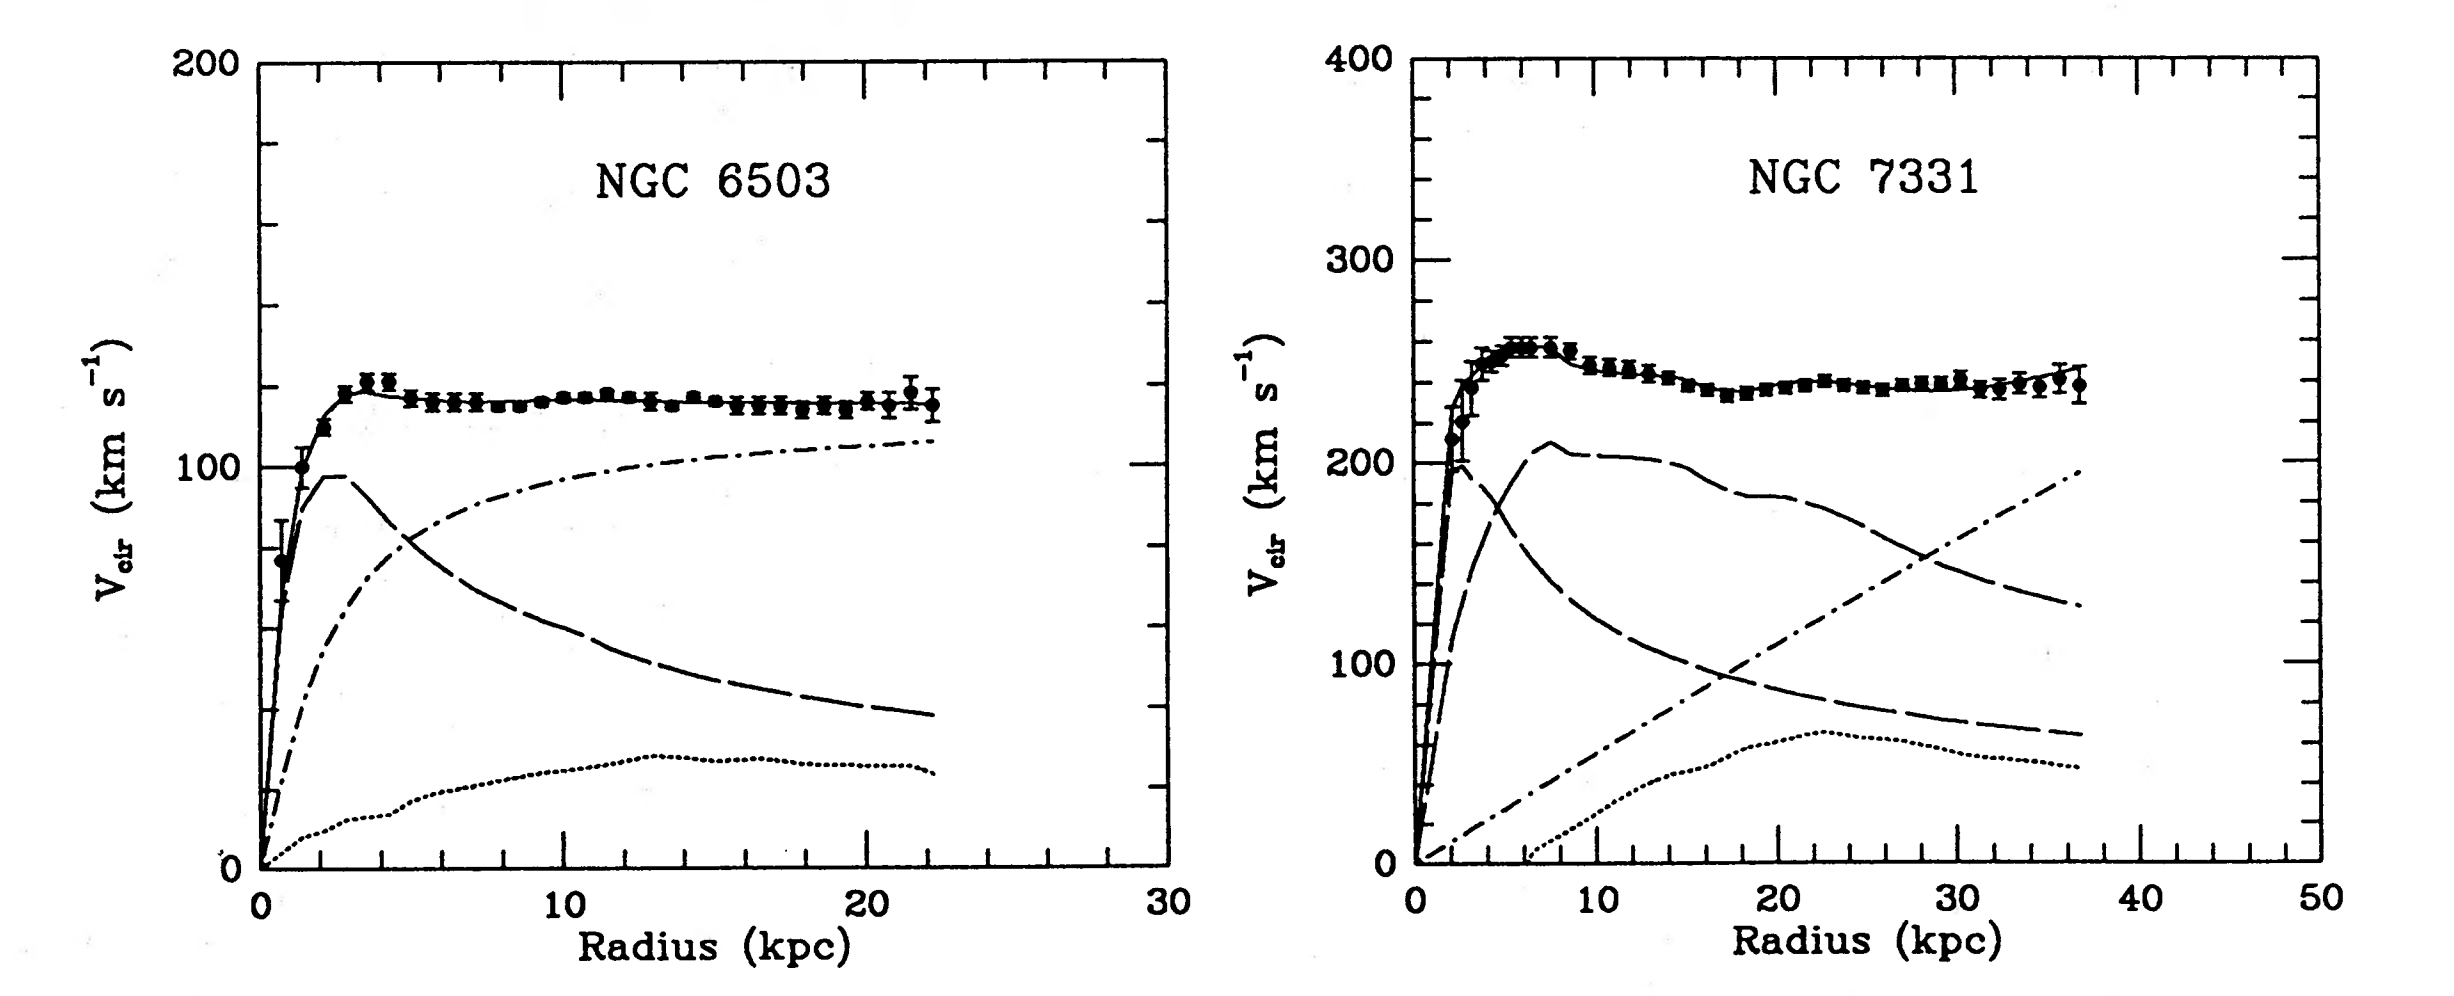
\includegraphics[width=0.85\textwidth]{Motivation/Figures/rotation_curves.png}
  \caption{
    The observed (points) and fitted (solid line) rotation curves for two sample galaxies.
    The fit consists of three components: the stellar component (dashed), the interstellar gas (dotted), and the dark matter halo (dash-dotted).
    Reprinted from Reference~\cite{}. % http://adsabs.harvard.edu/abs/1991MNRAS.249..523B
  }
  \label{fig:rotation_curves}
\end{figure}



\subsection{Dark Matter Candidates}
\label{sec:dm_cand}

WIMPs and axions for now.

\subsection{Non-collider Searches}
\label{sec:dm_search}

Describes.

\subsection{Simplified Models for LHC}
\label{sec:dm_simp}

It was the hot thing at the time.

% \chapter{The CMS Detector}
\label{sec:cms}

The Compact Muon Solenoid (CMS) detector is one of two hermetic, general purpose detectors at the Large Hadron Collider.
The original motivation for the experiment was the discovery of the Higgs boson by observing its decays to photons, electrons, and muons.
Towards this end, the detector was built to fulfill the following goals:
\begin{itemize}
\item Unambiguous charge identification of muons with momenta up to 1\TeV
\item 1\GeV mass resolution on 100\GeV pairs of muons, electrons, and photons
\item Efficient triggering and tagging of $\tau$ lepton and $b$ quark decays
\item Good resolution on the hadronic energy and missing transverse energy
\item Sufficient time resolution to deal with 40 MHz of collisions
\end{itemize}
The CMS detector consists of four main subdetetors: the inner trackers, the electromagnetic calorimeter (ECAL), the hadronic calorimeter (HCAL), and the muon chambers.
The first three are within the field volume of the eponymous 3.8 T superconducting NbTi solenoid magnet while the muon chambers are embedded in the return yoke of the magnet.
Additionally, there is an online triggering system to reduce readout from 40 MHz to $\mathcal{O}(1)$ kHz for prompt reconstruction. 

\begin{figure}[htbp]
  \centering
  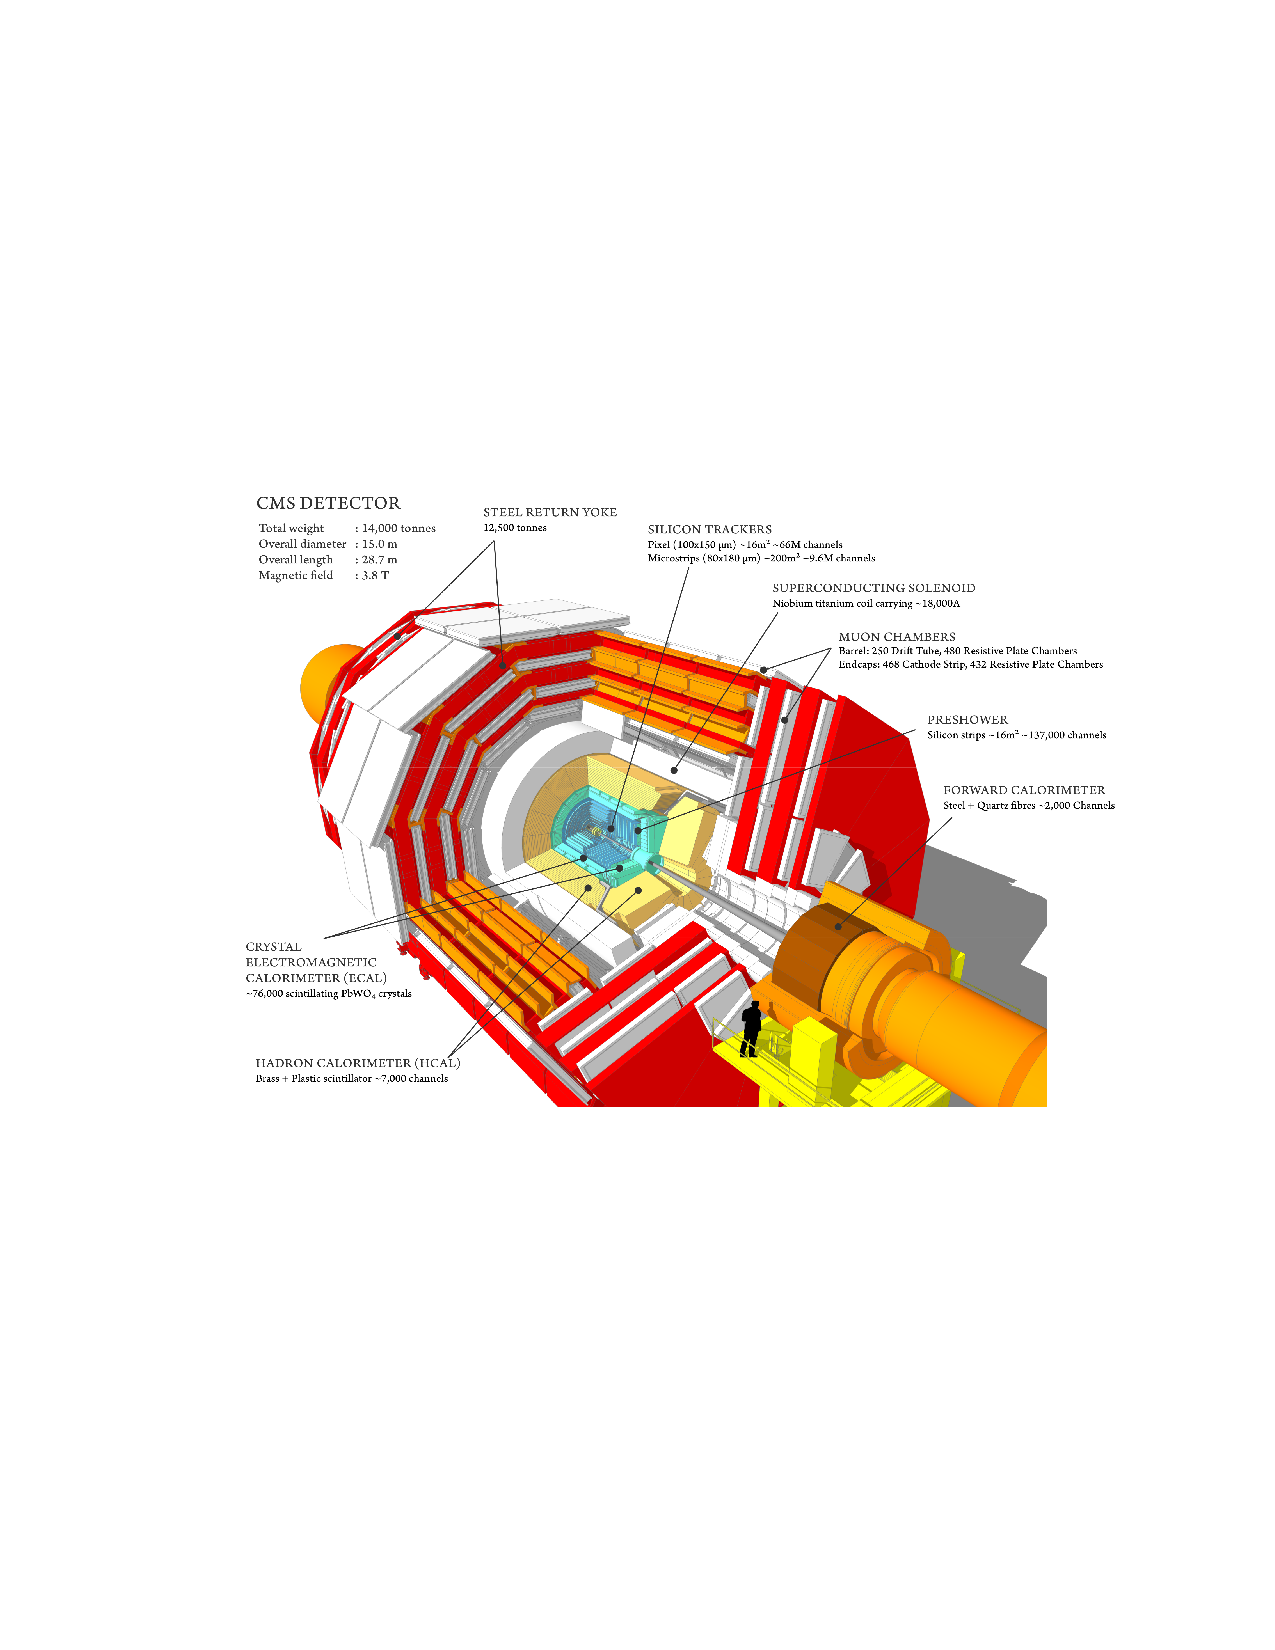
\includegraphics[width=0.9\textwidth]{Detector/Figures/cms_detector.pdf}
  \caption{
    A cutaway view of the CMS detector.
    The labels identify the solenoid as well as the different subdetectors and their components. 
    Reprinted from Reference~\cite{}. % http://cms.web.cern.ch/news/cms-detector-design
  }
  \label{fig:cms}
\end{figure}

The overall layout of the CMS detector is shown in Figure~\ref{fig:cms}. 
The CMS detector has a weight of 12500 tons, a length of 22 m, a diameter of 15 m, and a cylindrical geometry with concentric barrel shaped detectors in the central region and disc shaped detectors in the forward region.
The following coordinate system is used when working with the CMS detector:
\begin{itemize}
\item distance $z$ along the beam axis
  \begin{itemize}
  \item $z=0$ at the center of the detector
  \item positive corresponds to counter-clockwise as seen from the sky
  \end{itemize}
\item distance $r$ from the beam axis
\item polar angle $\theta$ measured with respects to the positive $z$-axis
\item azimuthal angle $\phi$ in the plane orthogonal to the beam axis
\end{itemize}
In addition to these four main coordinates, we define the right-handed cartesian $x$ and $y$ coordinates perpendicular to the beam axis, with the positive $x$-axis pointing from the center of the detector to the center of the LHC ring and the positive $y$-axis pointing upwards.

The four-momentum of a particle is $p = (p_x, p_y, p_z, E)$ in the cartesian basis 
%, where the first three components are space-like and the last one is time-like,
and a particle of mass $m$ produced at rest in the center of the detector has $p = (0, 0, 0, m)$.
While the momenta along the beam axis of the two incoming protons are equal, the momenta of the incoming partons involved in the hard scattering often are not as discussed in Section~\ref{sec:collider_pheno}.
Thus, we define two kinematic quantities that are Lorentz-invariant with respect to a boost along the beam axis:
the tranverse momentum $\ptvec = p_x \hat x + p_y \hat y$ with magnitude $\pt = \sqrt{p_x^2 + p_y^2}$ and the pseudorapidity $\eta = - \ln \tan\sfrac{\theta}{2}$.

In terms of \pt, $\eta$, and $\phi$, we have the following expressions for our cartesian variables: $p_x = \pt \cos \phi$, $p_y = \pt \sin \phi$, $p_z = \pt \sinh \eta$, and $E = \pt \cosh \eta$, with the last equality assuming the mass of the particle is negligible compared to its momentum.
In terms of our Lorentz-invariant coordinates, the four-momentum of a given particle is $p = (\pt, \eta, \phi, E)$. 
Additionally, the spatial separation of two particles is given by $\Delta R = \sqrt{(\Delta\phi)^2 + (\Delta\eta)^2}$ and the fiducial acceptance of the CMS detector is from $0 \le \phi < 2\pi$ and $-5 \le \eta \le 5$.

\section{Inner Trackers}
\label{sec:cms_tracker}

Closest to the interaction point, the inner trackers identify charged particles and measures their momenta.
Additionally, high resolution tracks are used to identify primary and secondary vertices.
The magnetic field in the tracker volume is uniform with strength 3.8 T and field lines parallel to the beam direction. 
The tracker volume extends to 1.2 m in $r$ and 2.9 m in $z$, providing coverage for $\abs\eta < 2.5$,  and is instrumented with silicon pixels and strips.
Each silicon sensor is a $p$-$n$ semiconductor junction with a bias voltage applied.
When a charged particle passes through the depletion region of the junction, electron-hole pairs are produced and collected by the readout electronics.
A schematic of the inner tracker system is shown in Figure~\ref{fig:cms_tracker}.

\begin{figure}[htbp]
  \centering
  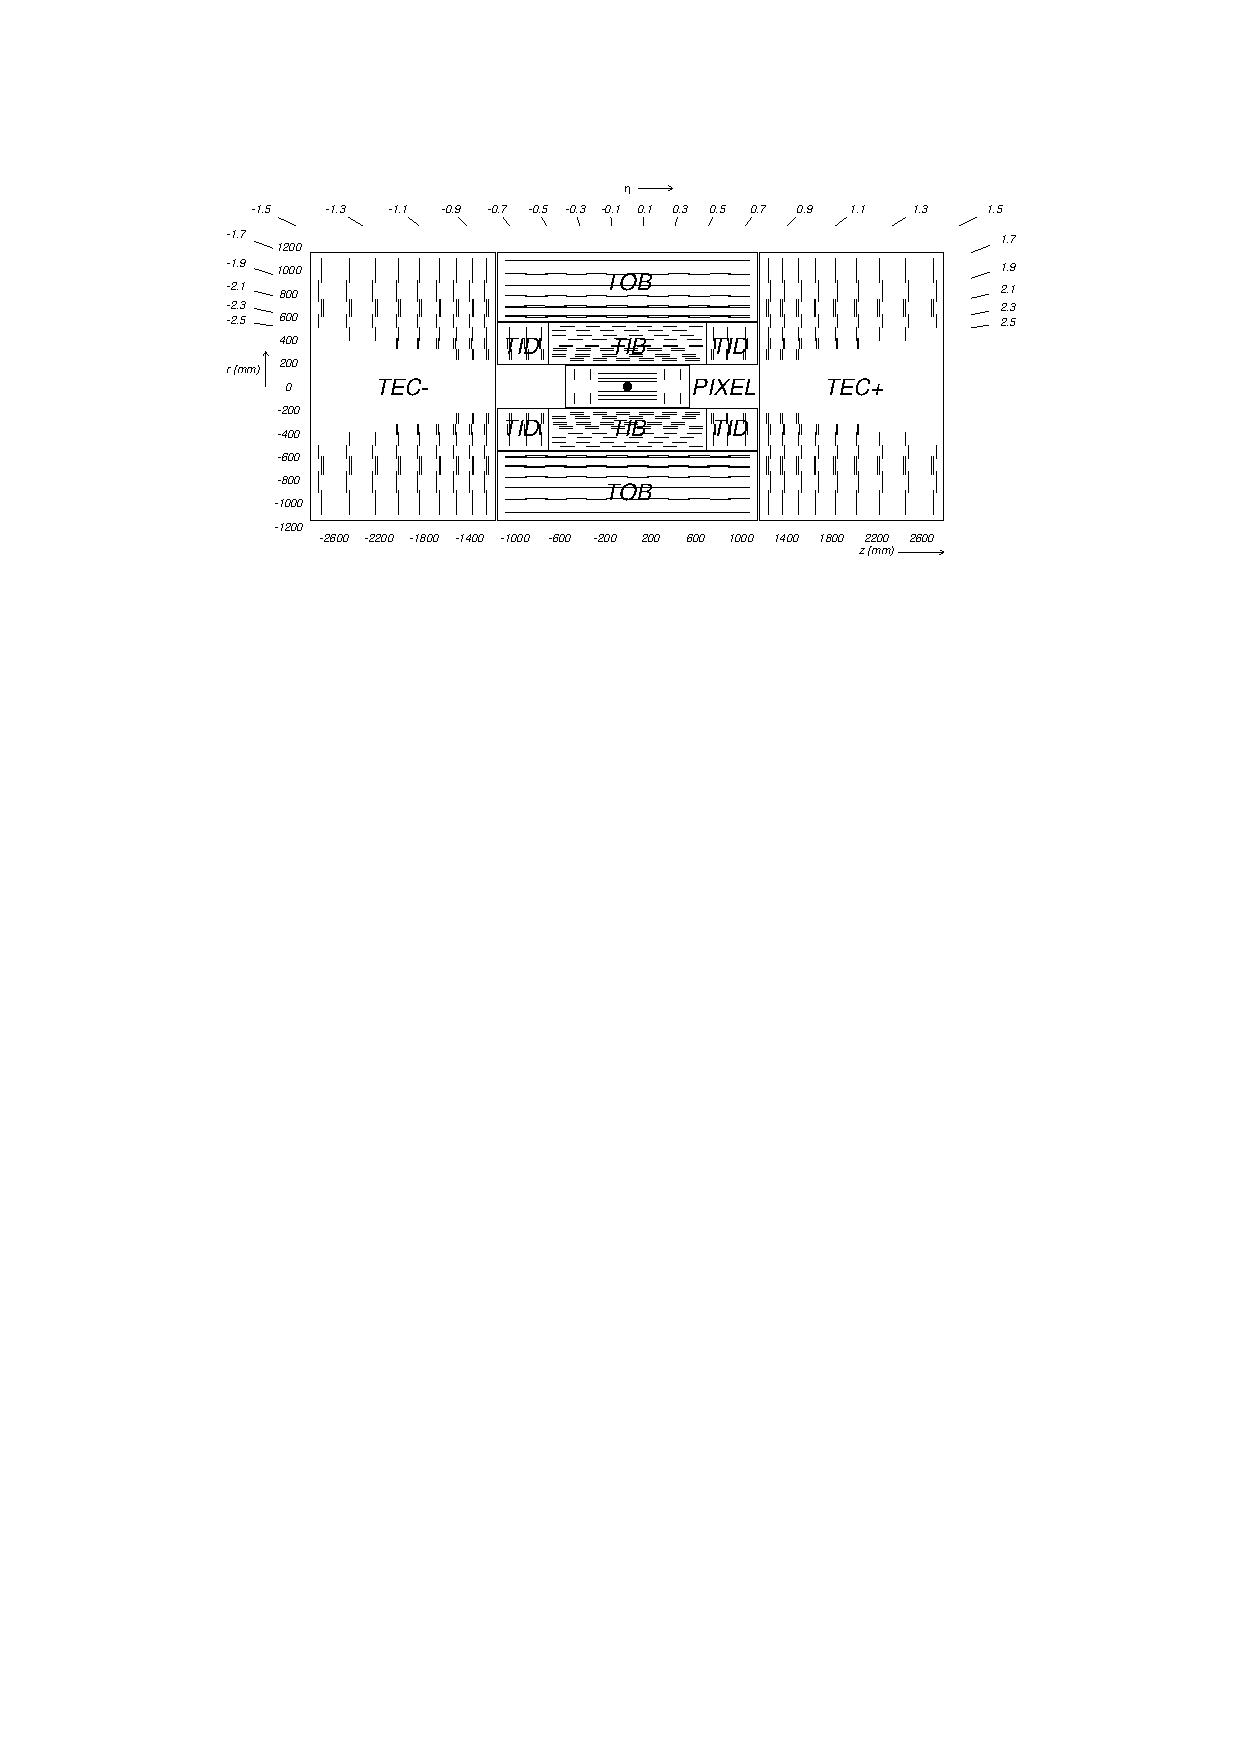
\includegraphics[width=\textwidth]{Detector/Figures/cms_tracker.pdf}
  \caption{
    A schematic view of the CMS inner tracker system.
    Silicon pixel and strip detectors are shown.
    The volumes labeled TIB, TID, TOB, and TEC are all strip trackers.
    The double lines indicate back-to-back modules that deliver stereo hits.
    % TIB = Tracker Inner Barrel, TID = Tracker Inner Disk, TOB = Tracker Outer Barrel, TEC = Tracker Endcap. 
    Reprinted from Reference~\cite{}. % https://iopscience.iop.org/article/10.1088/1748-0221/3/08/S08004/meta
  }
  \label{fig:cms_tracker}
\end{figure}

The 66 million individual pixel sensors, each measuring $285\mum\times 100\mum\times 150\mum$ in $r\times r\phi \times z$, are arranged into seven layers: three cylindrical barrels at $r = 4.4, 7.3, 10.2\cm$ and two bi-layer endcap annulli at $z = \pm34.5, \pm46.5 \cm$.
Due to the geometry of the pixel detector, tracks typically cross the sensor at a 20$^\circ$ angle, leading to the charge deposit from a single track to be shared among multiple pixels in the same layer.
The exact position of a particle in each layer is determined by interpolating the signals from multiple adjacent pixels with an analog pulse height greater than a tuneable read-out threshold.
Thus, each pixel hit is localized to an area of $\sim 15 \mum\times 20\mum$ in $r\phi \times z$, providing a much higher spacial resolution than the raw pixel spacing.

The pixels are surrounded 9.3 million silicon strips measuring $10\cm\times 80\mum$ arranged in ten cylindrical layers in the barrel and twelve disks in each endcap.
The Tracker Inner Barrel (TIB) consists of the first four layers and extends from 20\cm to 55\cm in the radial direction while out six layers constitute the Tracker Outer Barrel (TOB) with an outer radius of 116\cm and extent in $\abs z$ of 118\cm.
The remaining area in the barel is covered by the Tracker Inner Disk (TID), consisting of the three disks located from 80 to 90\cm in $\abs z$.
The Tracker EndCaps (TEC) have nine disks each and cover the region $124\cm < \abs z < 282\cm$.

The majority of the strips are oriented perpendicular to the $\phi$ direction: parallel to the beam pipe in the barrel region and radially aligned in the endcap region.
The strip pitch varies from 80 to 184\mum with the smallest pitch in the innermost layer.
This detector geometry provides good resolution in the $r$-$\phi$ plane for barrel and the $z$-$\phi$ plane for the endcap but little information on the orthogonal directions.
To compensate for this, one third of the strips are double-layered with a stereo angle of 100 mrad between the layers.
Matching hits between adjacent layers enables a measurement of the $z$ and $r$ coordinates in the barrel and endcap, respectively.
The final spacial resolution is 10-50\mum in the direction perpendicular to the strips and 100-530\mum in the parallel direction on the stereo modules.

% potential paragraph on tracker thickness

\section{Electromagnetic Calorimeter}

The electromagnetic calorimeter (ECAL) is a homogeneous, hermetic calorimeter
composed of 76,000 lead tungstate (PbWO4) crystals.
High density (8.3 g/$\cm^3$) lead tungstate was chosen due to its radiation hardness, fast scintillation decay time constant of 25\ns, small Moliere radius $r_M= 21.9\mm$, and short radiation length $X_0 = 8.9\mm$.
All of these factors combine to enable the construction of a compact calorimeter with high granularity and excellent energy resolution.

\begin{figure}[htbp]
  \centering
  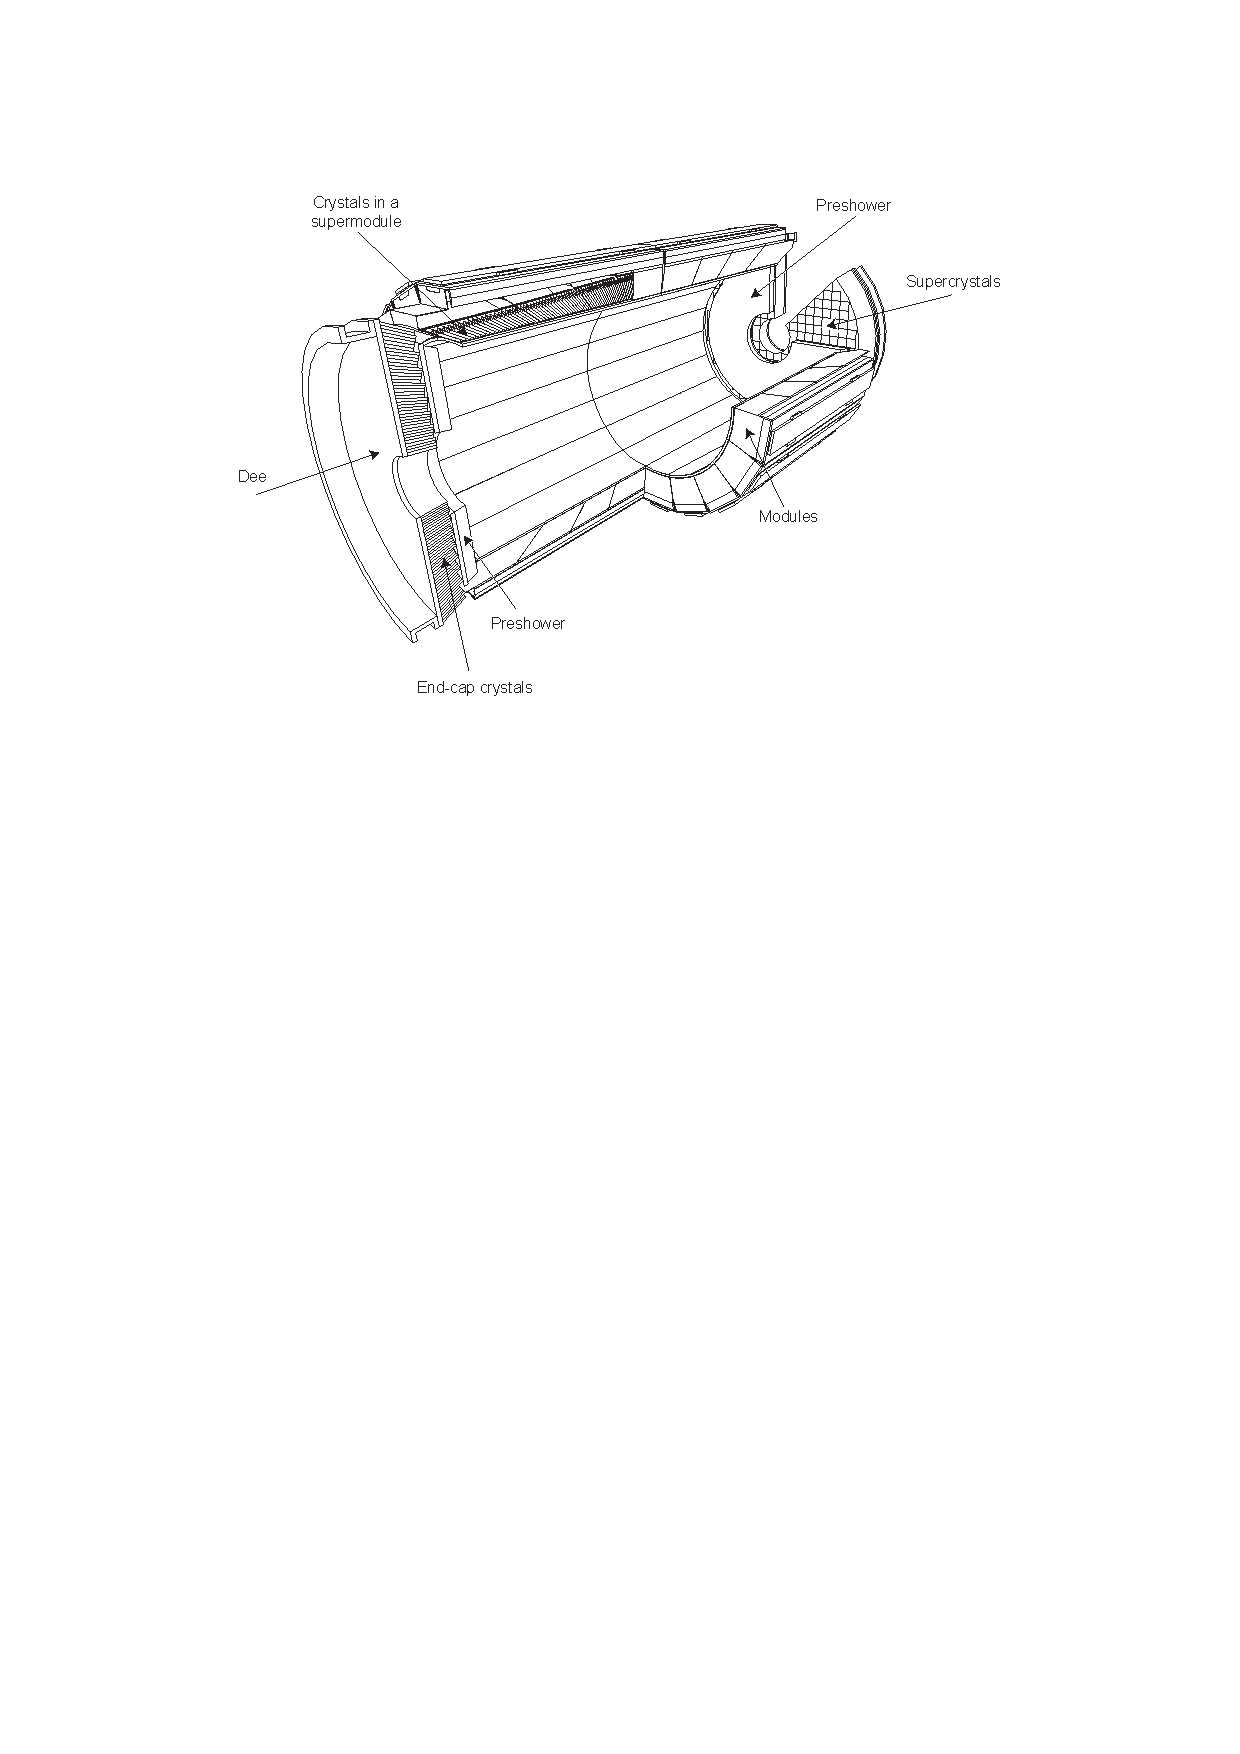
\includegraphics[width=0.9\textwidth]{Detector/Figures/cms_ecal.pdf}
  \caption{
    The layout of the CMS electromagnetic calorimeter.
    The barrel and endcap calorimeters are shown.
    The pre-shower detector sits in front of the endcaps.
    Reprinted from Reference~\cite{}. % https://iopscience.iop.org/article/10.1088/1748-0221/3/08/S08004/meta
  }
  \label{fig:cms_ecal}
\end{figure}

Figure~\ref{fig:cms_ecal} shows the layout of the ECAL.
The central barrel region (EB) has 61200 crystals arranged in a $170\times360$ $\eta$-$\phi$ grid ($0.0174\times0.0174$ granularity) with a coverage up to $\abs\eta = 1.44$ while the two endcap annuli (EE) each have 7324 crystals organized in a $x$-$y$ grid with coverage in the range $1.479 < \abs\eta < 3.0$.
Each crystal in the EB has a truncated pyramidal shape with a length of 230\mm, a $22\mm \times 22\mm$ front-face cross-section, and a $26\mm \times 26\mm$ rear-face cross-section while a crystal in the EE has a cuboid-like shape with a length of 220\mm, a $28.6 \mm \times 28.6\mm$ front-face cross-section, and a $30\mm \times 30\mm$ rear-face cross-section. 
The cross-sectional area of approximately one Moliere radius and length of approximately 25 radiation lengths allows just a few crystals to contain the entire transverse and longitudinal development of the shower.
To reduce the likelihood of the primary photon or electron emerging from the hard scattering depositing most of its energy in passive material, the crystals do not point directly to the interaction region.

The interactions between the 3.8 T magnetic field and the geometries of the ECAL lead to the selection of different photosensors in the barrel and endcaps.
In the endcaps, the magnetic field is parallel to the path of the photoelectrons and has a negligible effect on the gain, while in the barrel, the magnetic field is perpendicular and reduces the gain by a factor proportional to the distance traveled by the photoelectrons.
Thus, in the barrel, solid-state reverse-structure avalanche photodiodes (APDs) with a depletion layer of $6.0\pm0.5\mum$ are used, while photomultiplier tubes with a single gain stage and a very fine copper mesh anode called vacuum phototriodes (VPTs) are used in the endcaps. 
Two APDs with an active area of $25\mm^2$ are glued to the rear of each crystal in the barrel while only one VPT with an active area of $280\mm^2$ is needed per crsytal in the endcap.
The APDs and VPTs amplify the initial signal of approximately 4.5 photoelectrons per \MeV of energy deposit per crystal by a factor of 50 and 10, respectively. 

The small signals from the photodetectors are shaped and amplified in the Multi-Gain Preamplifier (MGPA) and a 12-bit analog-to-digital converter (ADC) samples the pulse every 25\ns.
Each output voltage pulse has a length of approximately 300\ns, with the maximum at approximately 75\ns\ and a slow decay afterwards. 
The MGPA has multiple gain modes of 12, 6, and 1, and the gain chosen for the output decreases once the signal has saturated the previous gain setting.
After the pulse falls below the saturation threshold, the lower gain setting is maintained for the next five samples.
This mechanism provides a dynamic signal range from a few MeV to a maximum of1.5\TeV in the barrel and 3.1\TeV in the endcaps.

The energy resolution of the ECAL was measured using an electron beam to be
\begin{equation}
  \frac{\sigma_E}{E} = \frac{2.8\%}{\sqrt{E/\GeV}} \oplus \frac{12\%}{E/\GeV} \oplus 0.3\%,
\end{equation}
where $E$ is the energy of the incident particle and the three terms on the RHS are the stochastic, noise, and constant terms, respectively.
The stochasistic term is dominated by event-to-event fluctuations in the lateral shower containment and a photostatistics contribution of 2.1\%.
Electronic and digitization noise drive the noise term while the constant term comes from a non-uniform longitudinallight collection and intercalibration errors.

\subsection{Preshower Detector}

At high momenta and high $\abs\eta$, the two photons from a $\pi^0$ decay can merge into a single ECAL crystal due to the large boost in the the $z$-direction of the initial state.
By forcing the initiation of an electromagnetic shower in a region with high spacial resolution in front of the ECAL endcaps, the preshower detector can differentiate between one- and two-photon deposits in the region $1.6 < \abs\eta < 2.5$.
The preshower detector consists of two alternating layers of passive lead absorbers and active silicon strip sensors.
The first (second) lead layer is two (one) radiation lengths thick and the subsequent sensor plane has vertical (horizontal) strips of 6\cm length and 1.9\mm pitch.
The silicon strips resolve the shower with a resolution of $\mathcal{O}(1-10)\mm$, enabling the disambigutation of two nearly collinear photons and the identification of $\pi^0$ decays.

\section{Hadronic Calorimeter}

The hadronic calorimeter (HCAL) is a set of four heterogenous calorimeters that provide hermetic coverage when combined:  the barrel calorimeter (HB) covering $\abs\eta< 1.3$, the endcap calorimeter (HE) covering $1.3 < \abs\eta < 3$, the outer calorimter (HO) covering $\abs\eta < 1.3$, and the forward calorimeter (HF) covering $3 < \abs\eta < 5$.
The region covering $\abs\eta < 3$ shall be referred to as the central HCAL.
The granularity of the HCAL in $\eta$-$\phi$ is $0.087\times0.087$ for $\abs\eta<1.6$, $0.17\times0.17$ for $1.6 < \abs\eta < 3.0$, and $0.175\times0.175$ for $3 < \abs\eta < 5$.
The layout of the HCAL is shown in Figure~\ref{fig:cms_hcal}. 

\begin{figure}[htbp]
  \centering
  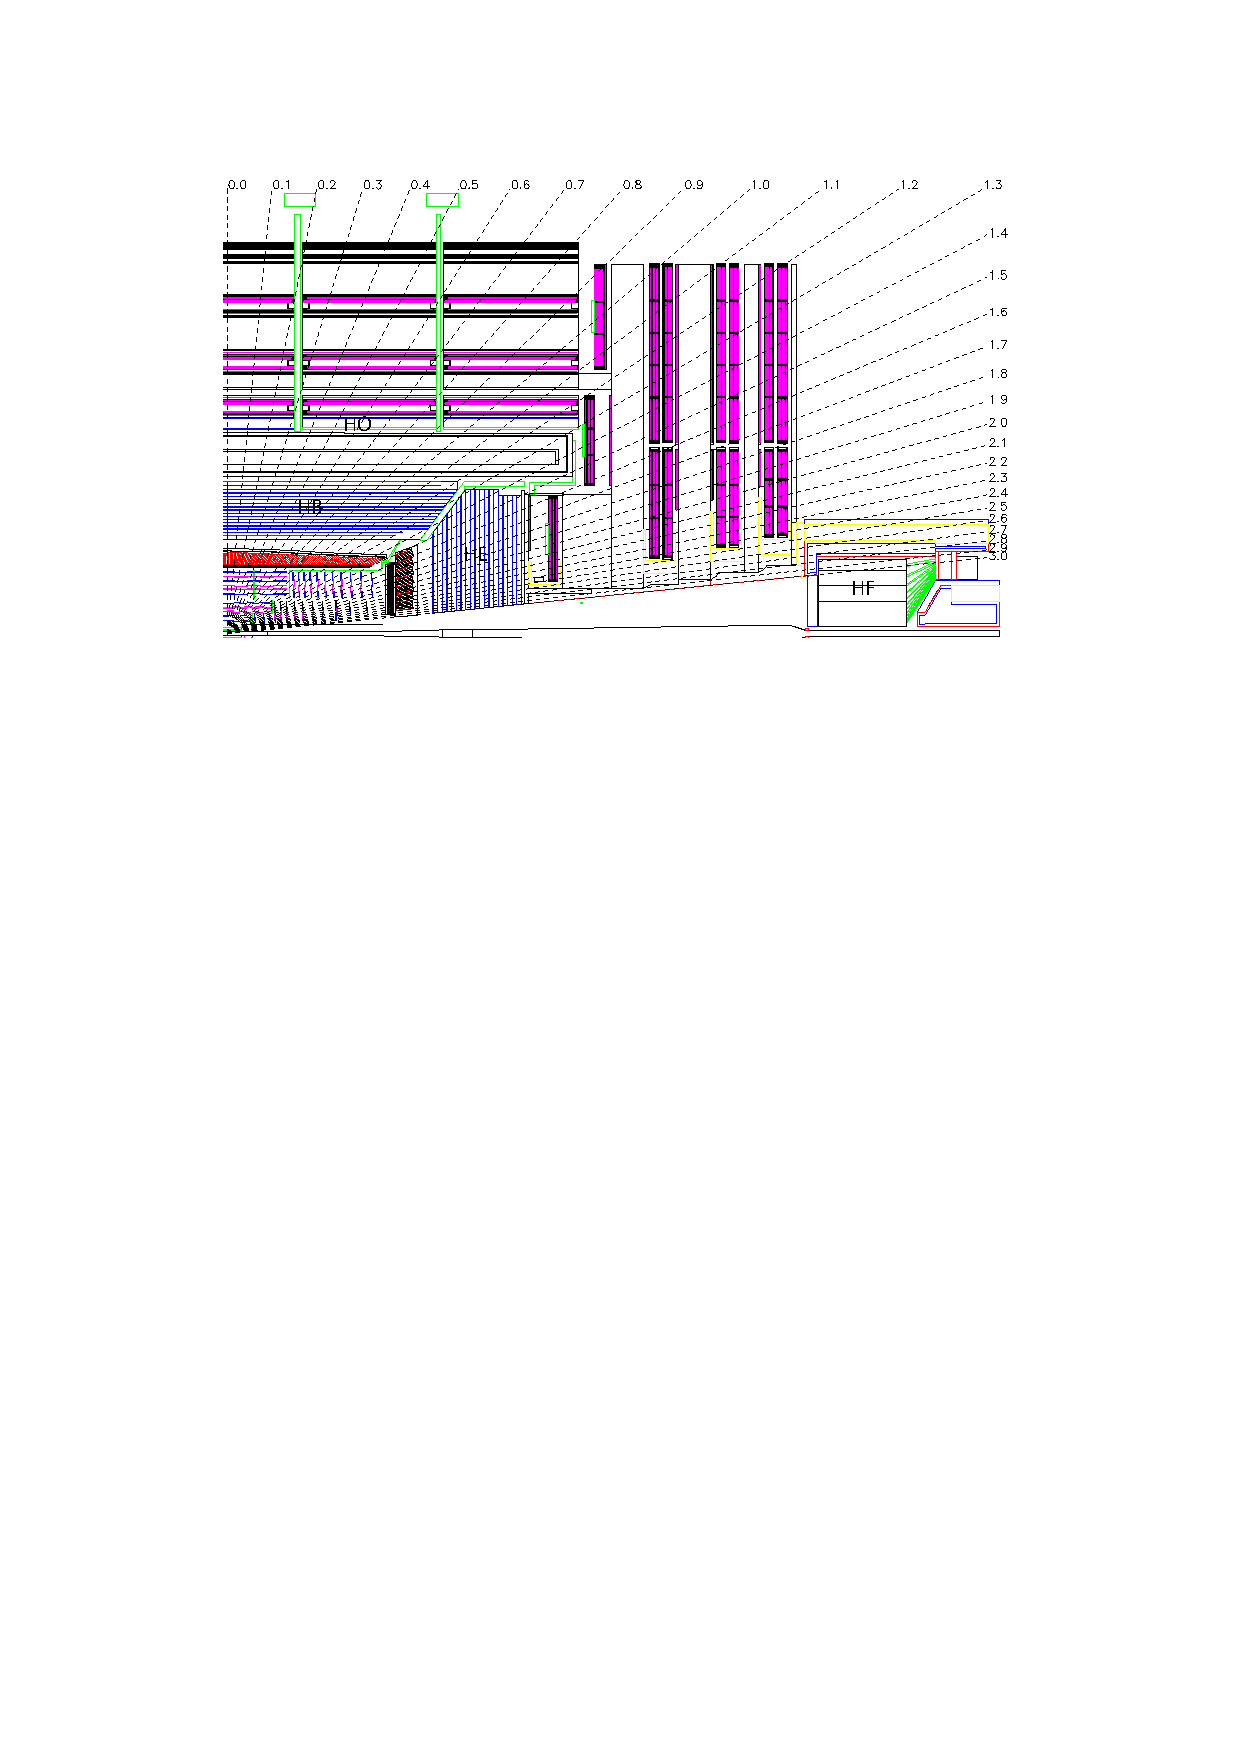
\includegraphics[width=\textwidth]{Detector/Figures/cms_hcal.pdf}
  \caption{
    The layout of the CMS hadronic calorimeter.
    The barrel, endcap, outer, and forward calorimeters are shown and labeled.
    The muon chambers are shown but not labeled. 
    The dashed lines denote different values of pseudorapidity.
    Reprinted from Reference~\cite{}. % https://iopscience.iop.org/article/10.1088/1748-0221/3/08/S08004/meta
  }
  \label{fig:cms_hcal}
\end{figure}

The HB and HE are sampling calorimeters with 16 and 17 thin plastic scintillator layers, respectively,  interleaved with thick absorber layers made of a non-magnetic brass alloy with an interaction length $\lambda_I = 1.5\cm$.
The layers range in thickness from 40 to 75\mm providing a total absorber depth ranging from a minumum of 5.82 $\lambda_I$ at $\abs\eta=0$ to a maximum of 10.6 $\lambda_I$ at $\abs\eta = 1.3$ in the barrel and approximately nine interaction lengths throughout the endcaps, with the ECAL contributing another interaction length worth of material.
The dimensions of the HB and HE are determined by the requirement that they reside between the ECAL and the solenoid. 
To circumvent this constraint, an additional layer of scintillator located in the return yoke of the magnet, the HO, utilizes the solenoid material as an additional interaction length of absorber.
Hybrid photodiodes (HPDs) are used to read out the scintillator light in the HB and HE while silicon photomultipliers (SiPMs) are used in the HO.

Located 11 meters from the interaction point, the HF is a sampling calorimeter covering the region of  phase-space with high pseudorapidity.
Since the particle flux here is much higher than in the central region, the HF uses radiation-hard steel absorber instrumented with two sets of scintillating quartz fibers.
Charged particles produced by showers in the steel traverse the quartz fibers and emit Cherenkov radiation that is recorded by photomultiplier tubes.
To distinguish hadrons from photons and electrons, the second set of fibers starts at a depth of 22\cm.

Since hadrons interact with the ECAL as well as the HCAL, the energy resolution of the detectors must be considered in tandem in the central region.
Using a charged particle test beam, the combined ECAL+HCAL energy resolution was measured to be
\begin{equation}
   \frac{\sigma_E}{E} = \frac{0.847}{\sqrt{E/\GeV}} \oplus 0.074
\end{equation}
and the standalone HF energy energy resolution is
\begin{equation}
   \frac{\sigma_E}{E} = \frac{1.98}{\sqrt{E/\GeV}} \oplus 0.09.
\end{equation}

\section{Muon Chambers}

The outer most components of CMS are the muon triggering, identification, and detection chambers.
These muon detectors are interleaved with the steel return yoke of the magnet resulting in a characteristic $S$-shape for the muon trajectories due to the reversal of magnetic field direction across the solenoid.
Signal purity in the muon detectors is high as hadrons, electrons, and photons are stopped by the calorimeters while muons are minimum ionizing particles (MIPs) that lose little energy while traversing the detector.
Taking advantage of the large detector volumes required by the outer solenoid radius of 3.5\unit{m}, three types of gas ionization chambers are used: drift tubes (DTs) in the barrel covering $\abs\eta < 1.2$, cathode strip chambers (CSCs) in the endcaps coering $0.9 < \abs\eta < 2.4$, and resistive plate chambers (RPCs) in both covering $\abs\eta < 2.1$.
The layout of the muon detectors is shown in Figure~\ref{fig:cms_muons}.

\begin{figure}[htbp]
  \centering
  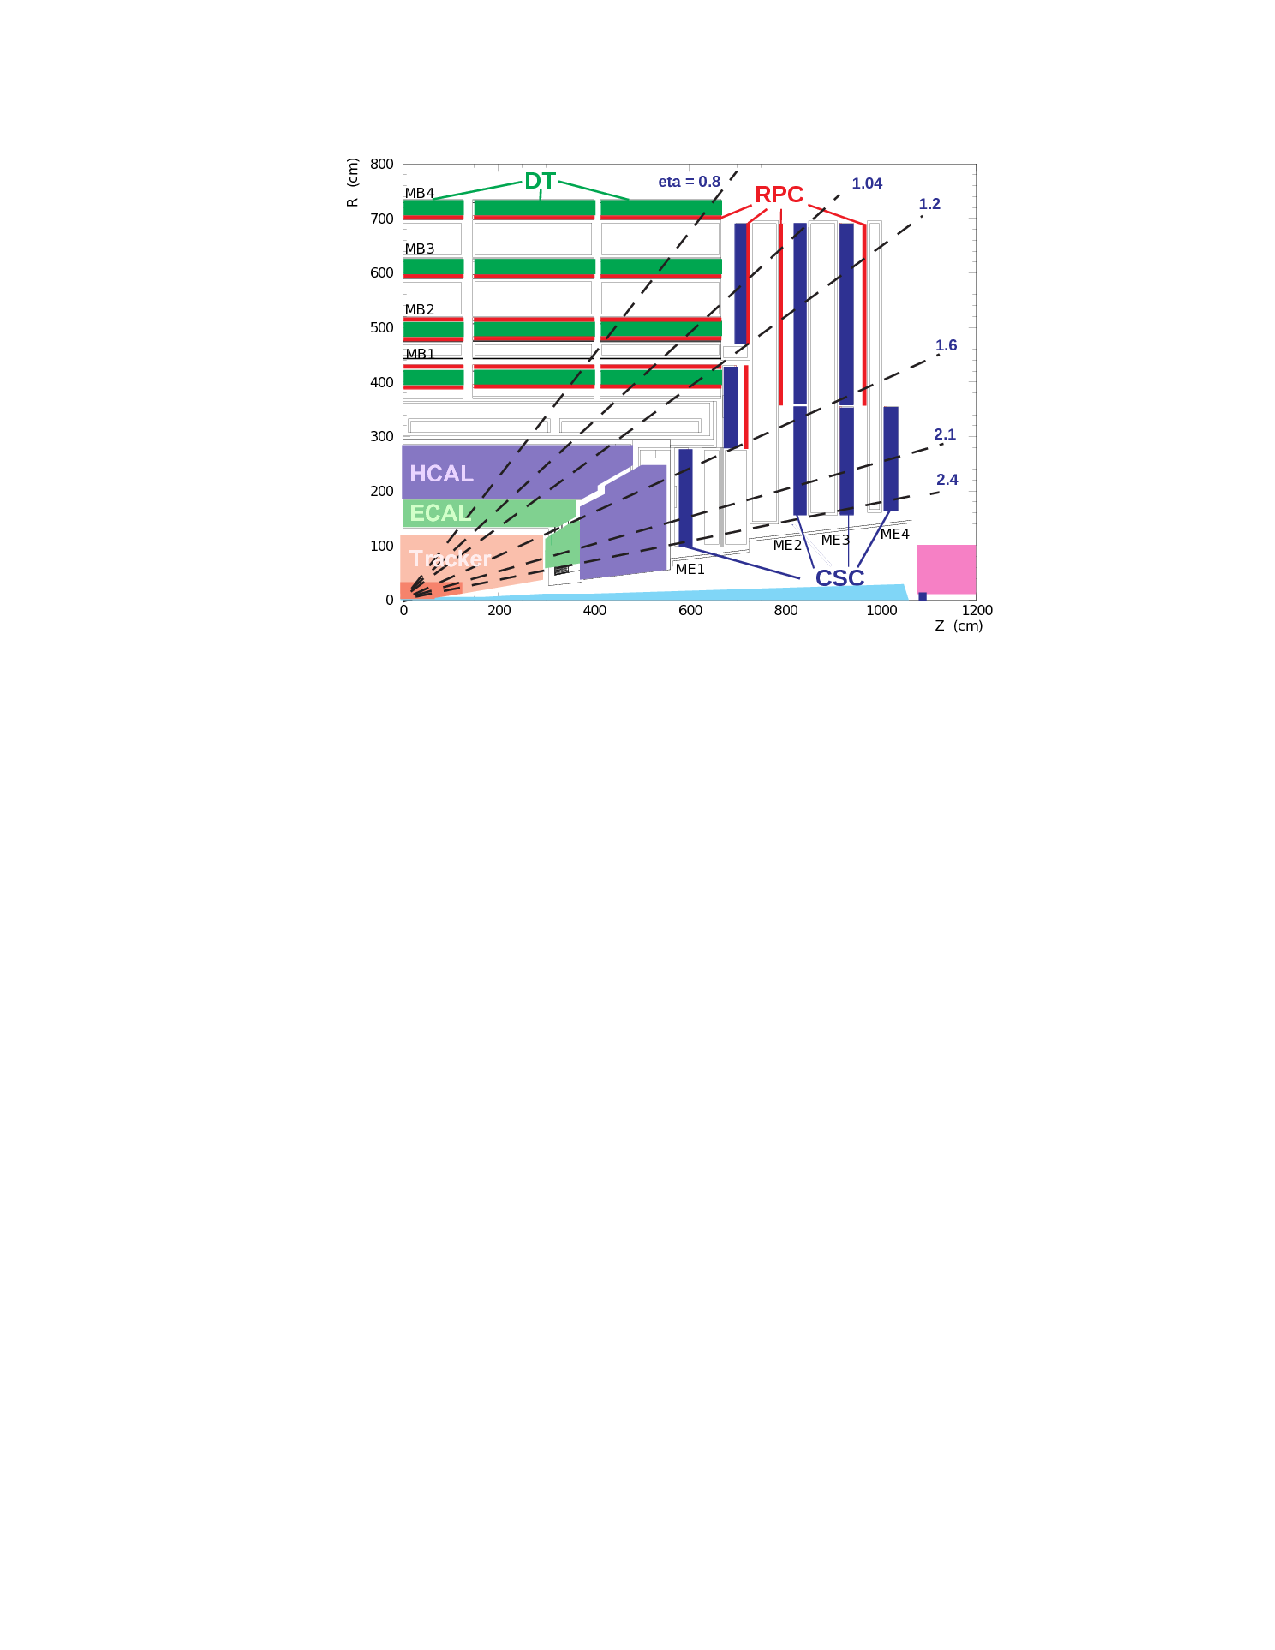
\includegraphics[width=0.9\textwidth]{Detector/Figures/cms_muons.pdf}
  \caption{
    The layout of the CMS muon chambers.
    The four DT stations are labeled MB1-MB4, the four CSC stations are labeled ME1-ME4, and the RPC stations are shown in red.
    The dashed lines denote different values of pseudorapidity.
    Reprinted from Reference~\cite{}. % 
  }
  \label{fig:cms_muons}
\end{figure}

The DT chambers consist of rectangular drift cells with tranverse dimensions of $42\mm \times 13\mm$ filled with a 85:15 Ar/CO$_2$ mix and a gold/steel anode wire held at a voltage of 3.6\unit{kV}.
The  maximum drift time per cell of 400\ns\ provides a spatial resultion of approximately 250\mum.
A single chamber is made out of superlayers which are in turn made out of four individual cells for a combined resultion of 100\mum.
The chambers are arranged into four 2.4\unit{m} thick dodecagonal rings called the muon barrel stations.
All four stations have two superlayers per chamber that measure position in the $r$-$\phi$ plane while the chambers in the inner three stations have an additional superlayer that measures position in the $r$-$z$ plane.
Together, the four muon stations and iron yokes form a wheel with one between the solenoid and the first iron layer, two in between the yokes, and one outside.
The outer barrel is composed of five wheels in total. 

Due to their faster response time and better spatial resolution, CSCs are used to handle the higher muon and background fluxes in the endcap region. 
Each CSC is filled with a 50:40:10 CO$_2$/Ar/CF$_4$ mix and instrumented with 80 cathode strips held at voltages of 2.9-3.6\unit{kV} relative to the gold-plated tungsten anode wires.
The strips run radially outward to measure position in the $r$-$\phi$ plane while the wires run perpendicular measure the $\eta$ and beam-crossing time of the muons.
The four muon stations in each endcap are made of CSCs arranged into annuli oriented perpendicular to the beam axis and interspersed between the flux return plates.
The three inner stations have multiple annuli with smaller ones fitting inside the larger ones while the fourth station only has one close to the beamline.

An RPC is a parallel-plate double-gap chamber with a time resolution of one nanosecond and a poor spatial resolution. 
The RPCs are interspersed throughout the DT and CSCs to provide an independent muon trigger system that can identify the correct bunch crossing time.

\section{Online Trigger System}

To achieve an instantaneous luminosity of $\mathcal{O}(10^{34}) \percms$, the LHC has bunch crossings every 25\ns\ for a total data rate of 40\unit{MHz}, much higher than the 100\unit{kHz} readout rate for the detector and the $\mathcal{O}(1)\unit{kHz}$ data reconstruction and tape writing rates.
Fortunately, uninteresting elastic scattering and QCD inelastic scattering events dominate the approximately 100\unit{$\mu$b} total proton-proton cross-section at the LHC.
Meanwhile, most new physics processes have a predicted on the order of picobarns or femtobarns and even the highest rate SM EWK cross-sections are $\mathcal{O}(10)$\unit{nb}, so not every event needs to be readout, reconstructed, and written to tape.

A two-stage trigger system selects the events to keep for permanent storage and analysis.
The Level 1 hardware-based trigger (L1) selects interesting events based on incomplete detector information to reduce readout and computation times.
Events selected by the L1 trigger are fully readout and passed to the high level software-based trigger (HLT) where the full event is reconstructed using the data acquisition system (DAQ), a computing farm with over 20k CPU cores.
Events selected by the HLT are sent to the offline computing resources for full reconstruction followed by storage on disk and tape. 

\begin{figure}[htbp]
  \centering
  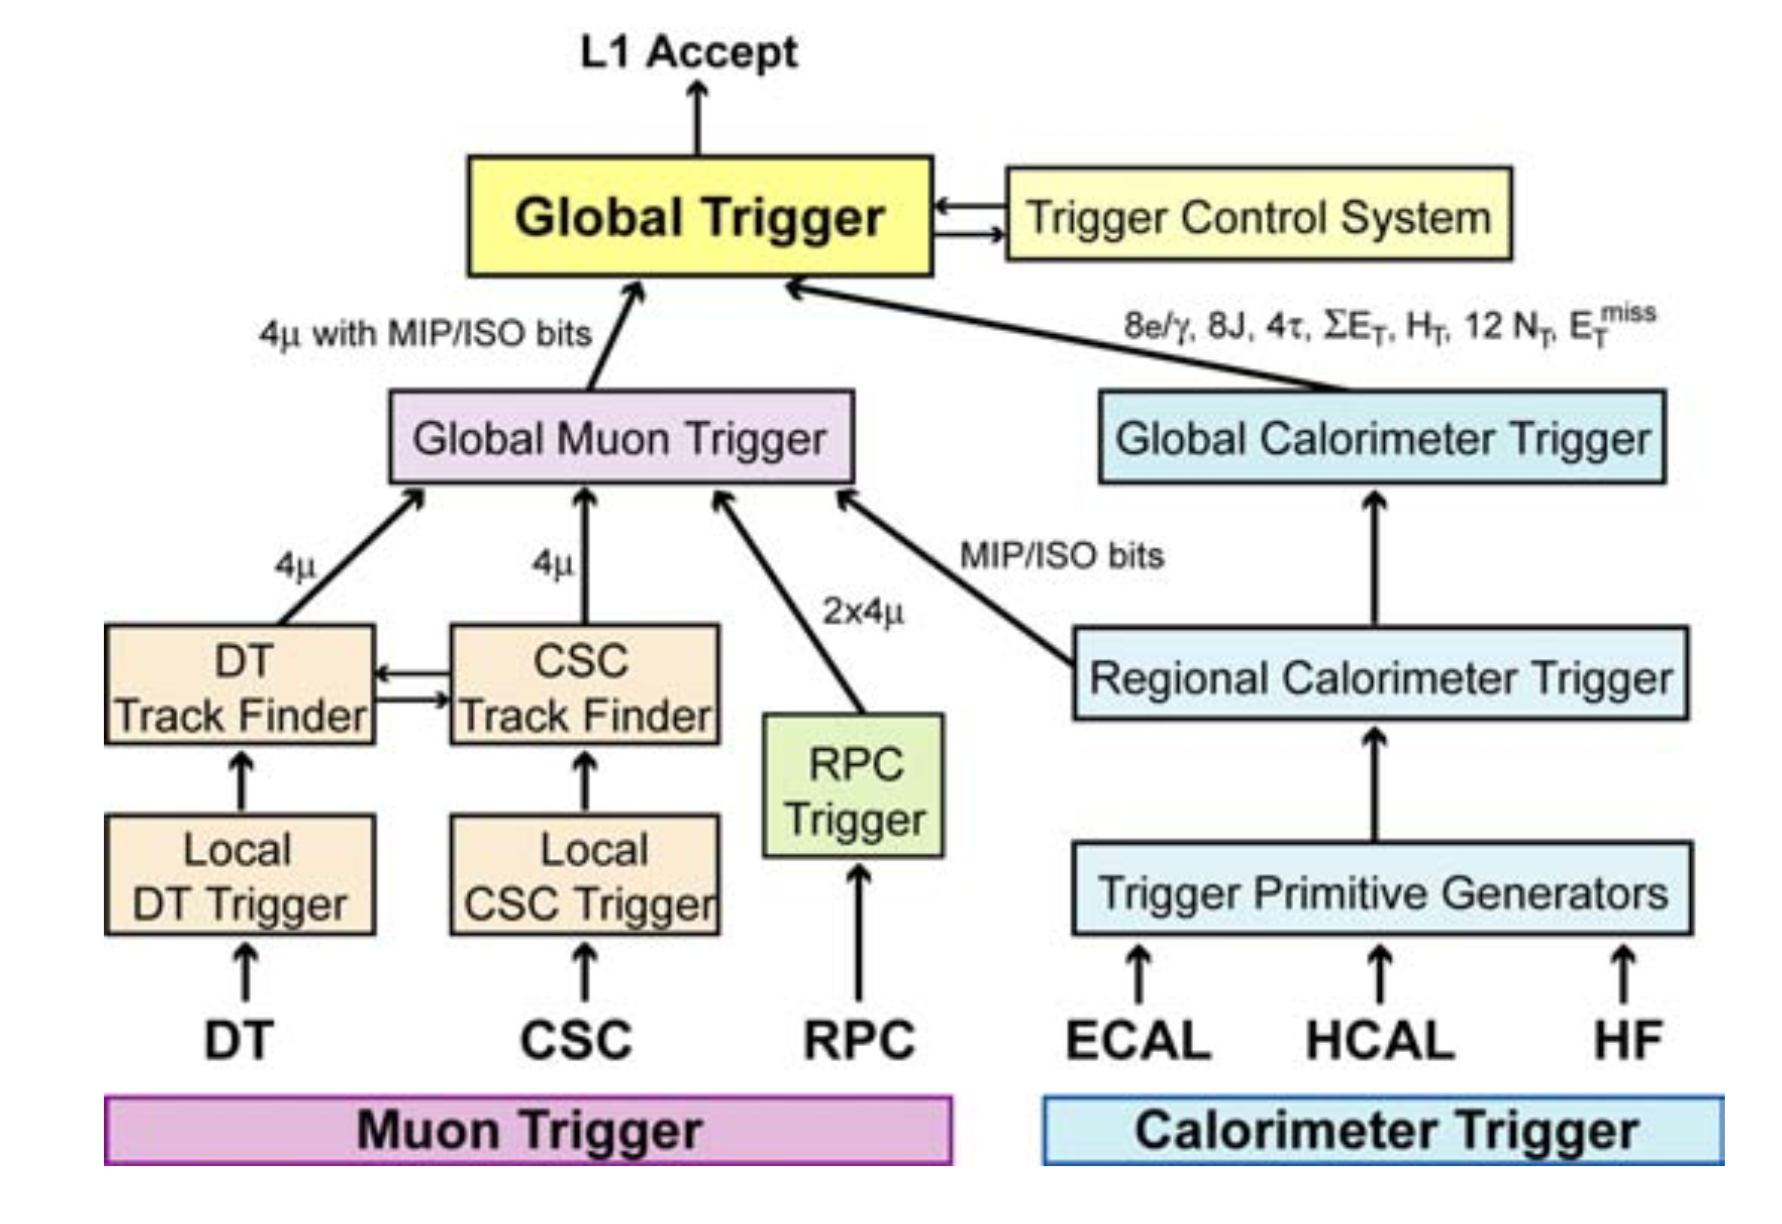
\includegraphics[width=0.8175\textwidth]{Detector/Figures/cms_l1t.png}
  \caption{
    The Level-1 trigger architecture with components labeled and information flow indicated.  
    Reprinted from Reference~\cite{}. % https://iopscience.iop.org/article/10.1088/1748-0221/3/08/S08004/meta
  }
  \label{fig:cms_l1t}
\end{figure}

The L1 trigger uses field programmable gate arrays (FPGAs) and application specific integrated circuits (ASICs) to make decisions within 4\mus of each collision.
Each subdetector module has a hardware trigger that reconstructs objects called trigger primitives (TPs).
In the two calorimeters, clustered energy deposits from each tower are sent to a regional calorimeter trigger (RCT) which correlates the information from adject towers and between the ECAL and HCAL into electron, photon, and jet candidates.
The outputs from the RCT are passed to the global calorimeter trigger (GCT) which computes global event variables such as the total transverse energy, the hadronic transverse energy, and the momentum imbalance.
Muon track candidates are produced from a simple segment-finding and tracking algorithm in each of the three types of muon chambers.
The global muon trigger (GMT) receives the candidates and combines them with information from the GCT to produce the final set of muon candidates.
The global trigger (GT) decides if an event should be sent to the HLT based on the information it receives from the GCT, the GMT, and the Timing, Trigger, and Control (TTC) system that monitors the readiness of the sub-detectors and the DAQ.
The inner tracker is not included because the detector readout and reconstruction process take longer than the time alloted.
Figure~\ref{fig:cms_l1t} shows a schematic description of the full L1 trigger process.

The HLT uses a version of the offline reconstruction software optimized to process a single event within 200\unit{ms} at the cost of some precision.
The reconstruction is split into a series of filters that make decisions within regions of interested defined by the L1 trigger infromation.
The HLT implements the desired trigger logic by constructing trigger paths out of these filters.
For example, three filters relevant for dark matter searches are (1) a single photon, (2) large momentum imbalance, and (3) large hadronic energy.
Combining the first two yields a trigger path targetting the monophoton channel while combining the latter two yields one for the monojet channel.
To reduce CPU usage, simple decisions such as those using only the calorimeters or muon information are computed before complex decisions such as tracking.

An event must pass all the filters in a given path to be recorded in an output primary dataset (PD).
Trigger paths are organized into PDs such that each PD contains events with similar topologies.
Some examples are the SinglePhoton, DoubleMuon, and Jet/HT datasets. 
A single event that exhibits multiple different physics signatures can pass multiple trigger paths and end up in multiple PDs.
These overlaps must be considered in the offline analysis.

\section{Detector Simulation}

The Geant4 program is used to simulate the detector response to the particles produced in collisions.
Starting with the output of the particle-level MC described in Section~\ref{sec:collider_pheno}, final state particles are propagated through the solenoid's magnetic field into the passive and active elements of the detector where energy deposition, decay, and showering are simulated.
Additional inelastic proton-proton collision are overlaid into an event to simulate the effects of pileup.
As the particles interact with the detector, the response of the readout electronics is simulated, including the effects of noise.
In order to miminize differences between simulated events and those from collisions, the reconstruction software and output format are the same for both up to the retention of additional truth information from the generators.


% \chapter{Global Event Reconstruction}

% https://doi.org/10.1088/1748-0221/12/10/P10003

In the previous chapter, we discussed the interactions of particles with the individual subdetectors and how these generate electrical signals.
Now, we shall discuss the reverse process, namely reconstructing the individual particles or physics objects from the electrical signals recorded by the subdetectors.

Traditionally, each class of physics object ia reconstructed using information from a single subdetector: muons from the muon chambers, isolated photons and electrons from the ECAL, jets and missing transverse energy from the HCAL, and secondary vertices from $\tau$ lepton and $b$ hadron decays from the tracker.
However, as depicted in Figure~\ref{fig:cms_slice}, each type of particle interacts with multiple different subdetectors and this information is lost unless the information from all the subdetectors is combined into a single global event description.

The particle flow (PF) algorithm leverages the fine angular granularity of the calorimeters and the excellent momentum resolution of the inner tracker and muon chambers to greatly improve the reconstruction of physics objects and include soft particles that would otherwise be ignored.
This is especially advantageous for jet energy measurements as roughly 62\% of the jet energy is carried by charged hadrons, approximately 27\% by photons, around 10\% by neutral hadrons, and about 1.5\% by neutrinos.

\begin{figure}[htbp]
  \begin{center}
    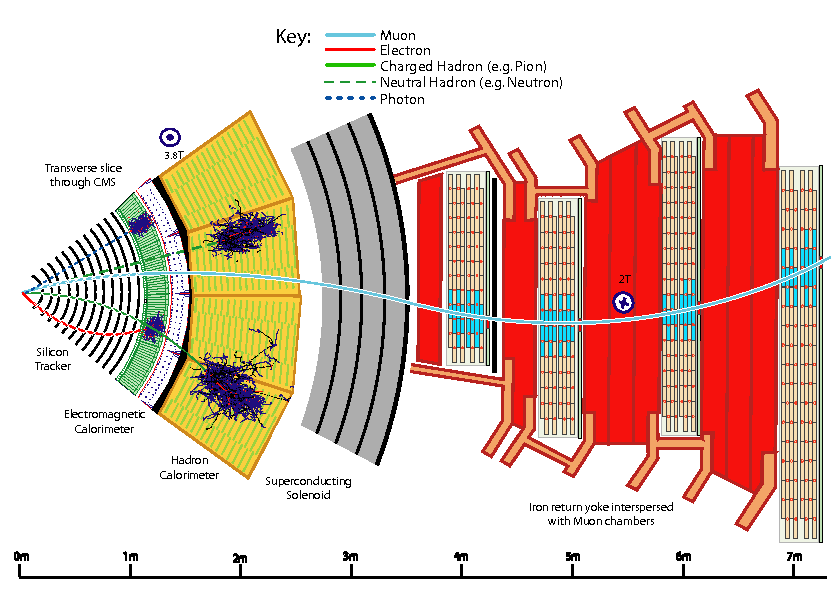
\includegraphics[width=0.875\textwidth]{Reconstruction/Figures/cms_slice.png}
    \caption{
      A sketch of a transverse slice of the CMS detector showing particle interactions from the interaction point to the muon detector.
      % Charge particles tracks are shown with solid lines while the paths of neutral particles are shown with dotted lines. 
      % The muon and charged pion are positively charged and the electron is negatively charged.
      % Neutrinos do not interact with the detector at an appreciably rate.
      Reprinted from Reference~\cite{}. % https://iopscience.iop.org/article/10.1088/1748-0221/12/10/P10003/meta
    }
    \label{fig:cms_slice}
  \end{center}
\end{figure}

The distinguishing feature of the PF algorithm is to combine multiple detector signals together into a single PF candidate.
The input detector signals are the tracks, vertices, calorimeter clusters, and muon segments described in Section~\ref{sec:pf_elements}.
Based on their proximity in the $\eta$-$\phi$, these PF elements are combined into muons, electrons, photons, and hadrons.
Muon segments are combined with inner tracks to produce muons, inner tracks are combined with calorimeter clusters to produce electrons and charged hadrons, and calorimeter clusters are correlated to produce photons and neutral hadrons.

The PF algorithm reconstructs particles in regions of the detectors called blocks following the steps described in Section~\ref{sec:pf_cands}.
After each step any PF elements associated to a PF candidate are removed from the block.
For example, clusters associated with photons will not be used when reconstructing neutral hadrons.
After all PF candidates are identified, they can be combined into event-wide variables such as jets and the missing transverse energy as described in Sections~\ref{sec:pf_jets} and~\ref{sec:pf_met}, respectively. 

\section{Particle Flow Elements}
\label{sec:pf_elements}

\subsection{Tracks}
\label{sec:pf_tracks}

% doi:10.1088/1748-0221/9/10/P10009

The Combinatorial Track Finder software is used to reconstruct tracks in an iterative inside-out process.
Initial interations search for tracks that are easy to find, e.g. those with high \pt, and hits associated with these tracks are removed for later iterations, reducing the combinatorial complexity and simplifying the search for more difficult tracks, e.g. greatly displaced ones.

The first step is to form seeds based on pixel hits, double strip hits containing 3D information, and an estimate of the beam spot.
Earlier iterations require three pixel hits while later iterations gradually loosen the requirements. %  to reconstruct displaced tracks.
The final iterations specifically target increased muon tracking efficiency by including information from the muon chambers.

Next, a Kalman filter is used to find additional hits consistant with the evolution of the track seeds through the rest of the tracker, accounting for the magnetic field, energy loss due to ionization, and multiple scattering.
The five parameters used for the helical trajectory evolution are the curvature $\rho$, the azimuthal angle $\phi_0$, the transverse impact parameter $d_0$ , the longitudinal impact parameter $z_0$ , and $\lambda = \cot \theta$, where $\theta$ is the polar angle.

After propagating the track through all layers of the detector and finding all associated hits, a Kalman fitter and smoother is used to refit the overall trajectory while a fourth-order Runge-Kutta method is used to extrapolate the trajectory between successive hits.
To reduce the fraction of fake tracks, various quality requirements concerning the number of missing hits, the reduced $\chi^2$ of the fit, and compatibility with a primary vertex are applied before proceeding to the next iteration.

% https://doi.org/10.1088/1748-0221/12/10/P10003

Track reconstruction for electrons is more complicated as the Kalman filter is not a good description because of the high rate of non-Gaussian energy loss due to brehmsstrahlung these tracks experience within the tracker.
To improve the electron reconstruction efficiency, the electron seed collection is filled both by looking outside-in for ECAL superclusters (see Section~\ref{sec:pf_sc}) consistant with track seeds and inside-out track seeds consistent with superclusters.
A Gaussian Sum Filter (GSF) defined to approximate the Bethe-Heitler energy-loss distribution is used to fit the trajectory of electron tracks. 

\subsection{Primary Vertexing}
\label{sec:pf_pv}

% doi:10.1088/1748-0221/9/10/P10009

A deterministic annealing (DA) algorithm is used to associate tracks to primary vertices.
Tracks must pass additional requirements on the transverse impact parameter $d_0$, the number of strip and pixel hits, and the reduced $\chi$ of the trajectory fit to be considered when finding primary vertices.
The most probable vertex positions at an artifical temperature $T$ are determined by the minimization of the ``free energy''
\begin{equation}
  F = -T \sum_i^{N_T} \ln \sum_j^{N_V} p_{ij} \rho_j \exp \left[ - \frac{1}{T} \left(\frac{z_i^T - z_j^V}{\sigma^z_i}\right)^2 \right]
\end{equation}
where the $z_j^V$ are the vertex positions with weights $\rho_j$, the $z_i^T$ and $\sigma_i^z$  are the longitudinal impact parameters and the corresponding uncertainties of the tracks, and the $p_{ij}$ are the probabilities of assigning the track $i$ of $N_T$ to the vertex $j$ of $N_V$.

The DA algorithm starts with a single vertex at a very high temperature that is gradually decreased.
The free energy $F$ is minimized with respects to $z_j^K$ at each new temperature and a vertex is split in two whenever $T$ falls below its criticial temperature
\begin{equation}
  T_C^j = 2 \sum_i \frac{p_i p_{ij}}{\left(\sigma_i^z\right)^2} \left(\frac{z_i^T - z_j^V}{\sigma^z_i}\right)^2 \Bigg/ \sum_i \frac{p_i p_{ij}}{\left(\sigma_i^z\right)^2}.
\end{equation}
The annealing procedure with vertex splitting continues down to $T = 4$ and the final assignment of tracks to vertices is performed at $T = 1$ without any further splitting. 
The vertex designated as \textit{the} primary vertex (PV) of the hard scattering is the one which maximizes
\begin{equation}
  S_T = \sum_i  (\pt^i)^2 + (\ptmiss)^2,
  \end{equation}
where $\pt^i$ is the transverse momentum of a track assigned to the vertex and \ptmiss\ is the magnitude of the momentum imbalance in the transverse plane for the vertex. 

\subsection{Secondary Vertexing}
\label{sec:pf_csv}

% https://arxiv.org/pdf/1712.07158.pdf

Long-lived particles such as $b$ hadrons and $\tau$ leptons often produce charged particles in their decays.
These charged particles are traced to a secondary vertex at the location of the decay, which is identified by the inclusive vertex fitter (IVF) algorithm.

The IVF procedure begins by selecting seed tracks with a 2D impact parameter significance $\sigma_{d_0} \ge 1.2$ and a 3D impact parameter $\sqrt{d_0^2 + z_0^2} \ge  50\mum$.
Tracks are assigned to a secondary vertex based on their opening angle with the seed track and distance at closest approach, with the additional stipulation that this distance be smaller for the secondary vertex than for the primary vertex.

To determine the precise position of the secondary vertices, the associated tracks are fitted with the adaptive vertex fitter and any vertices with a flight distance significance less than a certain threshold are discarded.
At this point, a track is unassociated from a secondary vertex if the angular distance between the track and the secondary vertex flight direction is greater than 0.4 and if the track's distance at closest approach is larger than the magnitude of its impact parameter.

The secondary vertex position is refitted after track cleaning if there are still at least two tracks associated with the vertex.
The last stage of cleaning removes a secondary vertex if it shares at least 20\% of its tracks with another and the flight distance significance between the two is less than ten.

\subsection{ECAL Superclusters}
\label{sec:pf_sc}

Due to the large amount of material in the tracker, electrons often emit bremsstrahlung photons, photons often convert to electron-positron pairs, and the brehmsstrahlung photons and converted electrons often undergo further conversion and brehmsstrahlung before reaching the ECAL.
Because of the bending of electron trajectories in the magnetic field, the resulting electromagnetic (EM) shower is significantly spread in the $\phi$-direction and collimated in the $\eta$-direction.
The ECAL reconstruction algorithm combines the basic cluster from each showered particle into a supercluster representing the initial electron or photon from the hard scattering. 

% https://iopscience.iop.org/article/10.1088/1748-0221/10/06/P06005/pdf

The first step is the identification of a seed crystal with greater transverse energy than its immediate neighbors and above a predefined minimum threshold.
The energy of each crystal is determined from calibration constants combined with the amplitude and peak time obtained by fitting the pulse shape of the ten time samples surrounding the triggering bunch crossing.

% https://iopscience.iop.org/article/10.1088/1748-0221/10/08/P08010/pdf

In the barrel, a supercluster starts with a $5\times1$ array of crystals in the $\eta$-$\phi$ plane centred on the seed crystal.
The array is extended around the seed crystal in the $\phi$-direction up to $\abs{\Delta\phi} \le 0.3$ if the energy of the additional crystals exceeds a certain threshold. 
The contiguous array is grouped into distinct basic clusters each containing a seed array with energy greater than another threshold.
The supercluster is the collection of basic threshold found in the $\eta$-$\phi$ region centered on the initial seed crystal.
Since the crystals in the endcaps are arranged in an $x$-$y$ grid, clustering here uses fixed $5\times5$ matrices of crystals. 
After a seed cluster is identified, additional, partially overlapping $5\times5$ matrices are added if their centroid lies within $\abs{\Delta\eta} \le 0.07$ and $\abs{\Delta\phi} \le 0.3$.
For uncoverted photons, both methods produce superclusters that are simple $5\times5$ matrices.

\subsection{HCAL Clusters}
\label{sec:pf_clusters}

% pf paper

The purpose of clustering in the HCAL is to measure the energy and direction of neutral hadrons, disentangle neutral hadrons from charged hadron energy deposits, and improve the energy measurement for charged hadrons with poorly reconstructed tracks.
Similar to the supercluster algorithm, a cluster in the HCAL is first identified by a seed cell with greater transverse energy than its immediate neighbors and above a predefined minimum threshold.
This seed is then grown into a topological cluster by adding cells with at least a corner in common with a cell already in the cluster and energy above twice the noise threshold.

An iterative Gaussian mixture model is used to break each topological cluster of M individual cells is broken into N energy deposits corresponding to individual particles, where N is the number of seeds.
Each energy deposit is modeled as a Gaussian distribution $\mathcal{N}$ with amplitude $A_i$, mean $\vec \mu_i$ in the $\eta$-$\phi$ plane, and width $\sigma$ fixed by the calorimeter resolution.
The expected fraction $f_{ji}$ of the energy $E_j$ measured in the cell at position $\vec c_j$ from the $i$th energy deposit is
\begin{equation}
  f_{ji} = \dfrac{\mathcal{N}\left(\vec c_j | A_i, \vec \mu_i, \sigma\right)}
  {\sum_k^N \mathcal{N}\left(\vec c_j | A_k, \vec \mu_k, \sigma\right)}.
\end{equation}
The amplitude and position of each energy deposit are determined by an analytical maximum-likelihood fit to be
\begin{equation}
  \begin{matrix}[l | r]
    A_i = \sum\limits_j^M f_{ji} E_j &
    \vec \mu_i = \sum\limits_j^M f_{ji} E_j \vec c_j
  \end{matrix}
\end{equation}
where the initial values are the energy and position of the seeds.
The process of calculating energy fractions $f_{ji}$ and fitting for the amplitudes $A_i$ and positions $\vec \mu_i$ is repeated until convergence, at which point they are taken as the cluster parameters.

\subsection{Muon Segments}
\label{sec:pf_segments}

Muon segments are reconstructed from the hits in the muon chambers using a Kalman filter in a similar manner to that described for the inner tracker in Section~\ref{sec:pf_tracks}.
A full track constructed in this way is referred to as a standalone muon.

\subsection{Isolation}
\label{sec:pf_iso}

While not a physics object persay, isolation is a key concept of the PF algorithm that  distinguishes prompt leptons and photons originating in the hard scattering from those originating in the decays of hardrons during the parton shower.
The latter are surrounded by a large amount of additional hadrons while the former have little hadronic activity in their vicinity, originating mainly from the pileup vertices.

The isolation of a prompt object is the total amount of energy due to additional particles within an annulus of radius $0.01 < \dR < 0.4$ around the prompt object, where the lower bound avoids including the prompt object and its radiation in the sum.
The isolation is calculated using either the raw energy deposits in the subdetectors or the four-momenta of the PF candidates surrounding the prompt object depending the stage of the PF algorithm.
Prompt objects are required to have an isolation value below a certain threshold, rejecting hadrons misidentified as leptons and photons as well as non-prompt leptons and photons.

The isolation calculation is usually split into three different components based on the types of particles that contribute energy.
The photon isolation \Ig\ is the \ET\ sum of the PF photons defined in Section~\ref{sec:pf_photons} while the charged hadron and neutral hadron isolations \ICH\ and \INH\ are the \pt\ sums of the PF charged and neutral hadrons defined in Section~\ref{sec:pf_hadrons}, with the additional stipulation that charged hadrons be associated with the primary vertex.

In events with very few tracks, such as one with a single high \pt\ photon and a large momentum imbalance, it is possible that the identified primary vertex does not correspond to the \Pp\Pp\ interaction from which the photon object originates because the photon does not figure into the primary vertex calculation from Section~\ref{sec:pf_pv}.
In such cases, the photon object can be surrounded by charged hadrons and still appear isolated under the standard charged hadron isolation.
A conservative measure to address such misidentification is to replace \ICH\ with the maximum of the PF charged hadron isolations computed over all reconstructed vertices, e.g. the maximum charged hadron isolation $\ICHmax = \max\limits_{\text{vertices}} \ICH$.

To reduce the pileup dependence of these variables, the median energy density $\rho$ of the pileup interactions in the isolation cone is calculated using the effective areas given in Table~\ref{tab:ea} and subtracted from each isolation sum.
Additionally, since the rate of the charged particles originating from pileup interactions is about twice as large as the corresponding rate of the neutral particles, the pileup isolation \IPU\ is defined as the half the \pt\ sum of the PF charged hadrons \textit{not} associated with the primary vertex.
Often selections are placed on the individual isolation components when selecting prompt photons, while the relative combined PF isolation
\begin{equation}
  \IPF = \bigg(\ICH + \max \Big\{0, \INH + \Ig - \IPU\Big\}\bigg) \bigg/ \pt^\ell
\end{equation}
is used when selecting prompt leptons.

\begin{table}[htbp]
  \begin{center}
    \begin{tabular}{l|r|r}
      Isolation & $\abs\eta < 1.0$ & $1.0 < \abs\eta < 1.479$  \\
      \hline
      \ICH\ &  &  \\
      \INH\ & 0.0597 & 0.0807 \\
      \Ig\ & 0.1210 & 0.1107 \\
      \ICHmax\ & 0.01064& 0.1026
    \end{tabular}
    \caption{Effective areas for isolations.} 
    \label{tab:ea}
  \end{center}
\end{table}

\section{Particle Identification}
\label{sec:pf_cands}

\subsection{Muons}
\label{sec:pf_muons}

The first step of the PF algorithm reconstructs three types of muon candidates: the standalone muons described in Section~\ref{sec:pf_segments}, outside-in global muons, and inside-out tracker muons.
To construct a global muon, the algorithm identifies an inner track consistent with the trajectory of a standalone muon evolved inwards using a Kalman filter similar to those discussed in Section~\ref{sec:pf_tracks}. 
After finding a match, a global muon candidate is created by combining the inner track with the standalone track with a second Kalman filter. 
Conversely, to construct a tracker muon, the algorithm identifies a muon segment consistent with the trajectory of a inner track with $\pt > 0.5\GeV$.
Global and tracker muons sharing the same inner track are merged into a single candidate.
For muons with $\pt < 200\GeV$, the muon momentum is that of the inner track, while the momentum is determined from a global fit of the muon chambers and inner tracker for muons with momentum above this threshold. 

Hadrons misidentified muons are rejected through two separate mechanisms. First, the isolation with respects to inner tracks and calorimeter deposits within $\dR < 0.3$ is required to be less than 10\% of the muon \pt.
Non-isolated muons are kept only if certain selections on the reduced $\chi^2$ of the track fit and the two impact parameters $d_0$ and $d_z$ are satisfied.
Finally, misidentified or misreconstructed muons can lead to a spurious imbalance in the transverse momentum.
The procedure used to identify and remove these muon candidates is described in Section~\ref{sec:pf_met}.
The total efficiency of muon reconstruction is 99\%.

The work described in this thesis only considers global muons with $\pt > 10\GeV$ and $\abs\eta < 2.5$.
This minimum requirement is only used to reject events containing a muon and is referred to as the veto muon ID. 
The loose muon ID adds the requirement that the relative combined PF Isolation $\IPF$ must be less than 0.25.
 must be less than 0.25.
In order for a muon to pass the tight ID, it must satisfy the following additional requirements:
$\pt > 30\GeV$,
relative combined PF Isolation $\IPF < 0.15$,
global-muon track fit reduced $\chi^2 < 10$,
at least one muon-chamber hit included in the global-muon track fit,
muon segments in at least two muon stations,
inner track has transverse (longitudinal) impact parameter $d_0 < 2\mm$ ($d_z < 5\mm$) with respects to the primary vertex,
at least one pixel hit ,
and more than five tracker layers with hits.

\subsection{Electrons}
\label{sec:pf_electrons}

Electron candidates are seeded from the GSF tracks described in Section~\ref{sec:pf_tracks} as long as the corresponding ECAL clusters are not linked to three or more additional tracks.
In each block, all ECAL clusters linked to either the supercluster (SC) or one of the GSF track tangents are associated with the candidate to ensure optimal energy containment.
Additional tracks linked to these clusters are associated if the track momenta and energies of any linked HCAL clusters are compatible with the electron hypothesis.
Any tracks and clusters belonging to identified photon conversions linked to the GSF track tangents are associated as well.  

To recover any energy lost during the association process, the total energy of the collected clusters is corrected with analytical functions of $E$ and $\eta$. 
For ECAL-based candidates, the sum of the energies measured in the HCAL cells within $\dR < 0.15$ of the supercluster must be less than 10\% of the supercluster energy.
The final energy of an electron candidate is a weighted average of the corrected ECAL energy and the momentum of the GSF track and the electron direction is that of its GSF track.

The work described in this thesis only considers electrons with $\pt > 10\GeV$ and $\abs\eta < 2.5$.
Additionally, electrons must pass further cuts on the following observables:
the energy-weighted cell width in the $\eta$-direction \sieie\ of the corresponding SC,
the \deta\ and \dphi\ between the SC seed crystal and the GSF track at the PV,
the energy ratio of $H/E$ of the corresponding ECAL and HCAL towers,
the relative combined PF Isolation \IPF,
the difference in energy measured in the tracker and the calorimeter $\abs{1/E - 1/p}$,
the number of missing hits in the inner tracker,
and the existence of a pair of tracks originating at a displaced vertex, indicting photon conversion.
The exact values of the cuts are tuned based on whether the electron is in the barrel or the endcap and to give desired signal efficiencies and background acceptance.
The loose ID is tuned to 90\% signal efficiency and 0.5\% background acceptance, while the tight ID is tuned to 70\% signal efficiency and 0.1\% background acceptance.

\subsection{Isolated Photons}
\label{sec:pf_photons}

Photon candidates are seeded from the ECAL superclusters (SCs) described in Section~\ref{sec:pf_sc} as long as they have no links to GSF tracks and $\ET > 10\GeV$. 
The same cluster and track association process described for electrons in Section~\ref{sec:pf_electrons} is used for photons, with the photon energy and direction being that of the final supercluster.
This is motivated by the observation that the additional energy corrections used to improve the photon energy resolution cause photon candidates with large cluster width to exhibit unphysical energies. 
Figure~\ref{fig:corr_vs_sieie} is a profile of the magnitude of the energy correction in bins of \sieie, the energy-weighted cell width in the $\eta$-direction.

\begin{figure}[htbp]
  \begin{center}
    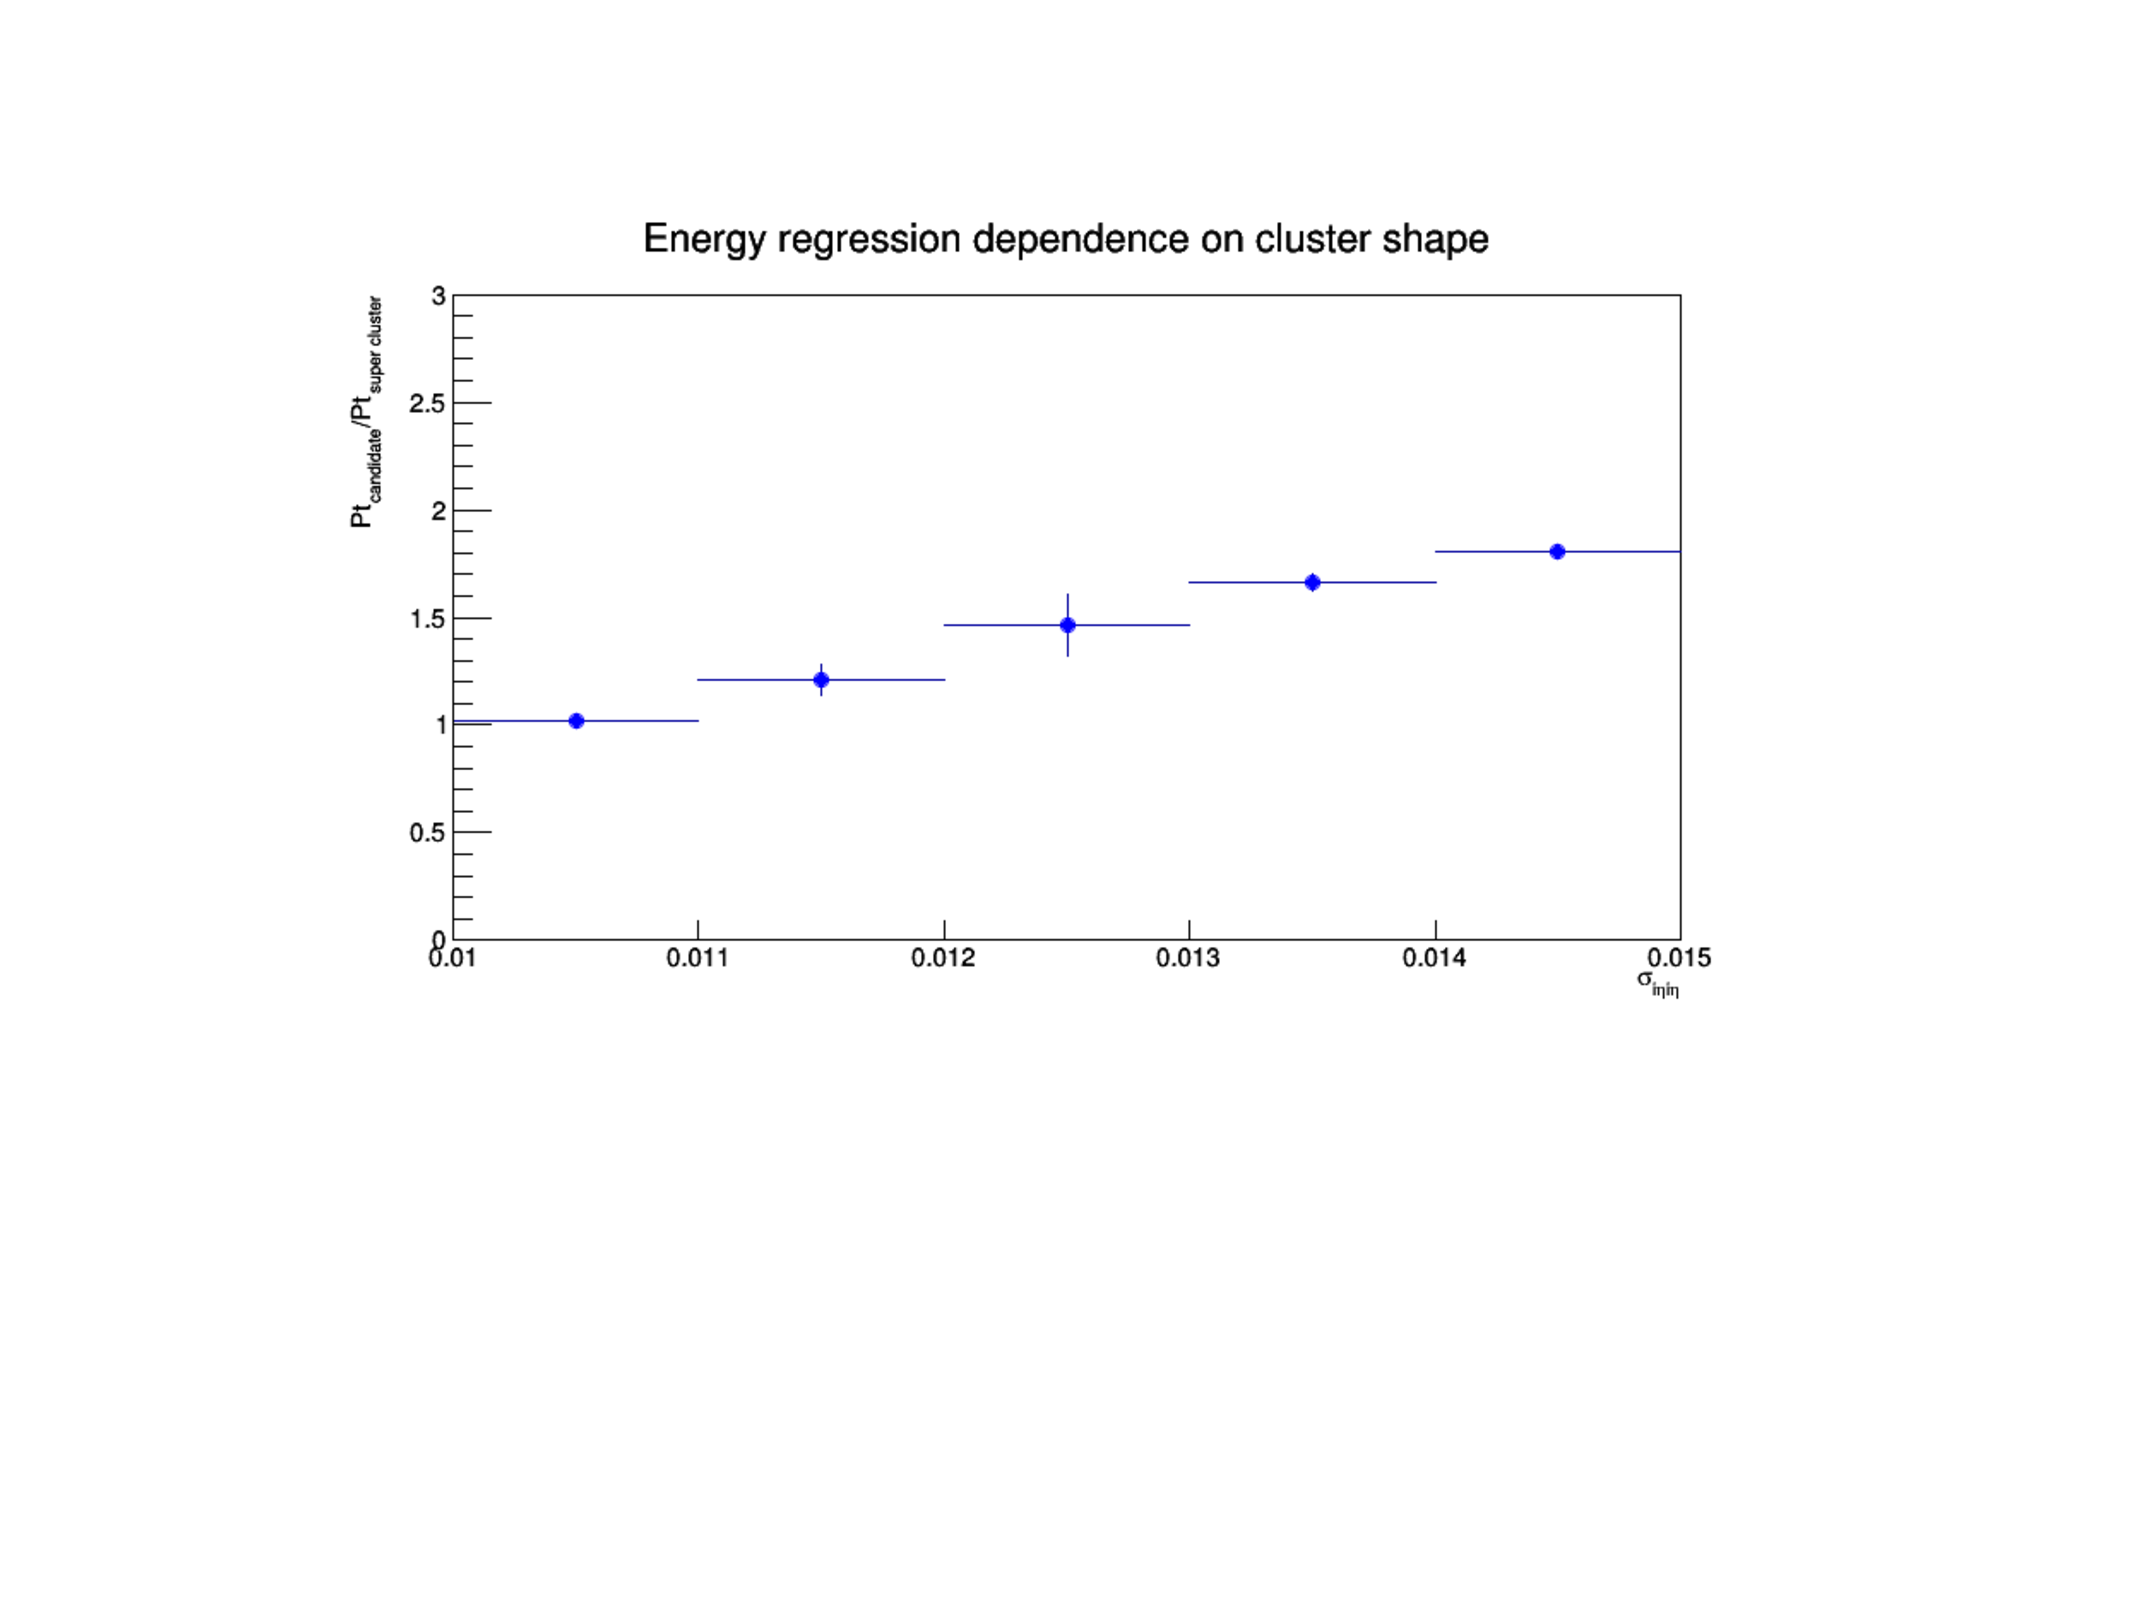
\includegraphics[width=0.6\textwidth]{Reconstruction/Figures/corr_vs_sieie.pdf}
    \caption{
      Magnitude of the energy correction on the photon object in bins of \sieie.
    }
    \label{fig:corr_vs_sieie}
  \end{center}
\end{figure}

As an illustration, an unphysically large correction is causing the transverse momentum of the photon object in the event shown in Fig.~\ref{fig:badcorr_evtdisp} to be nearly twice as large as the transverse momentum imbalance, which is supposed to balance the visible, \ie, photon momentum. 
Photon candidates with wide showers are used to estimate the hadron-to-photon misidentification background, while the photon energy resolution has an insignificant effect. 
Therefore, the unbiased supercluster energy was chosen over the corrected photon energy.

\begin{figure}[htbp]
  \begin{center}
    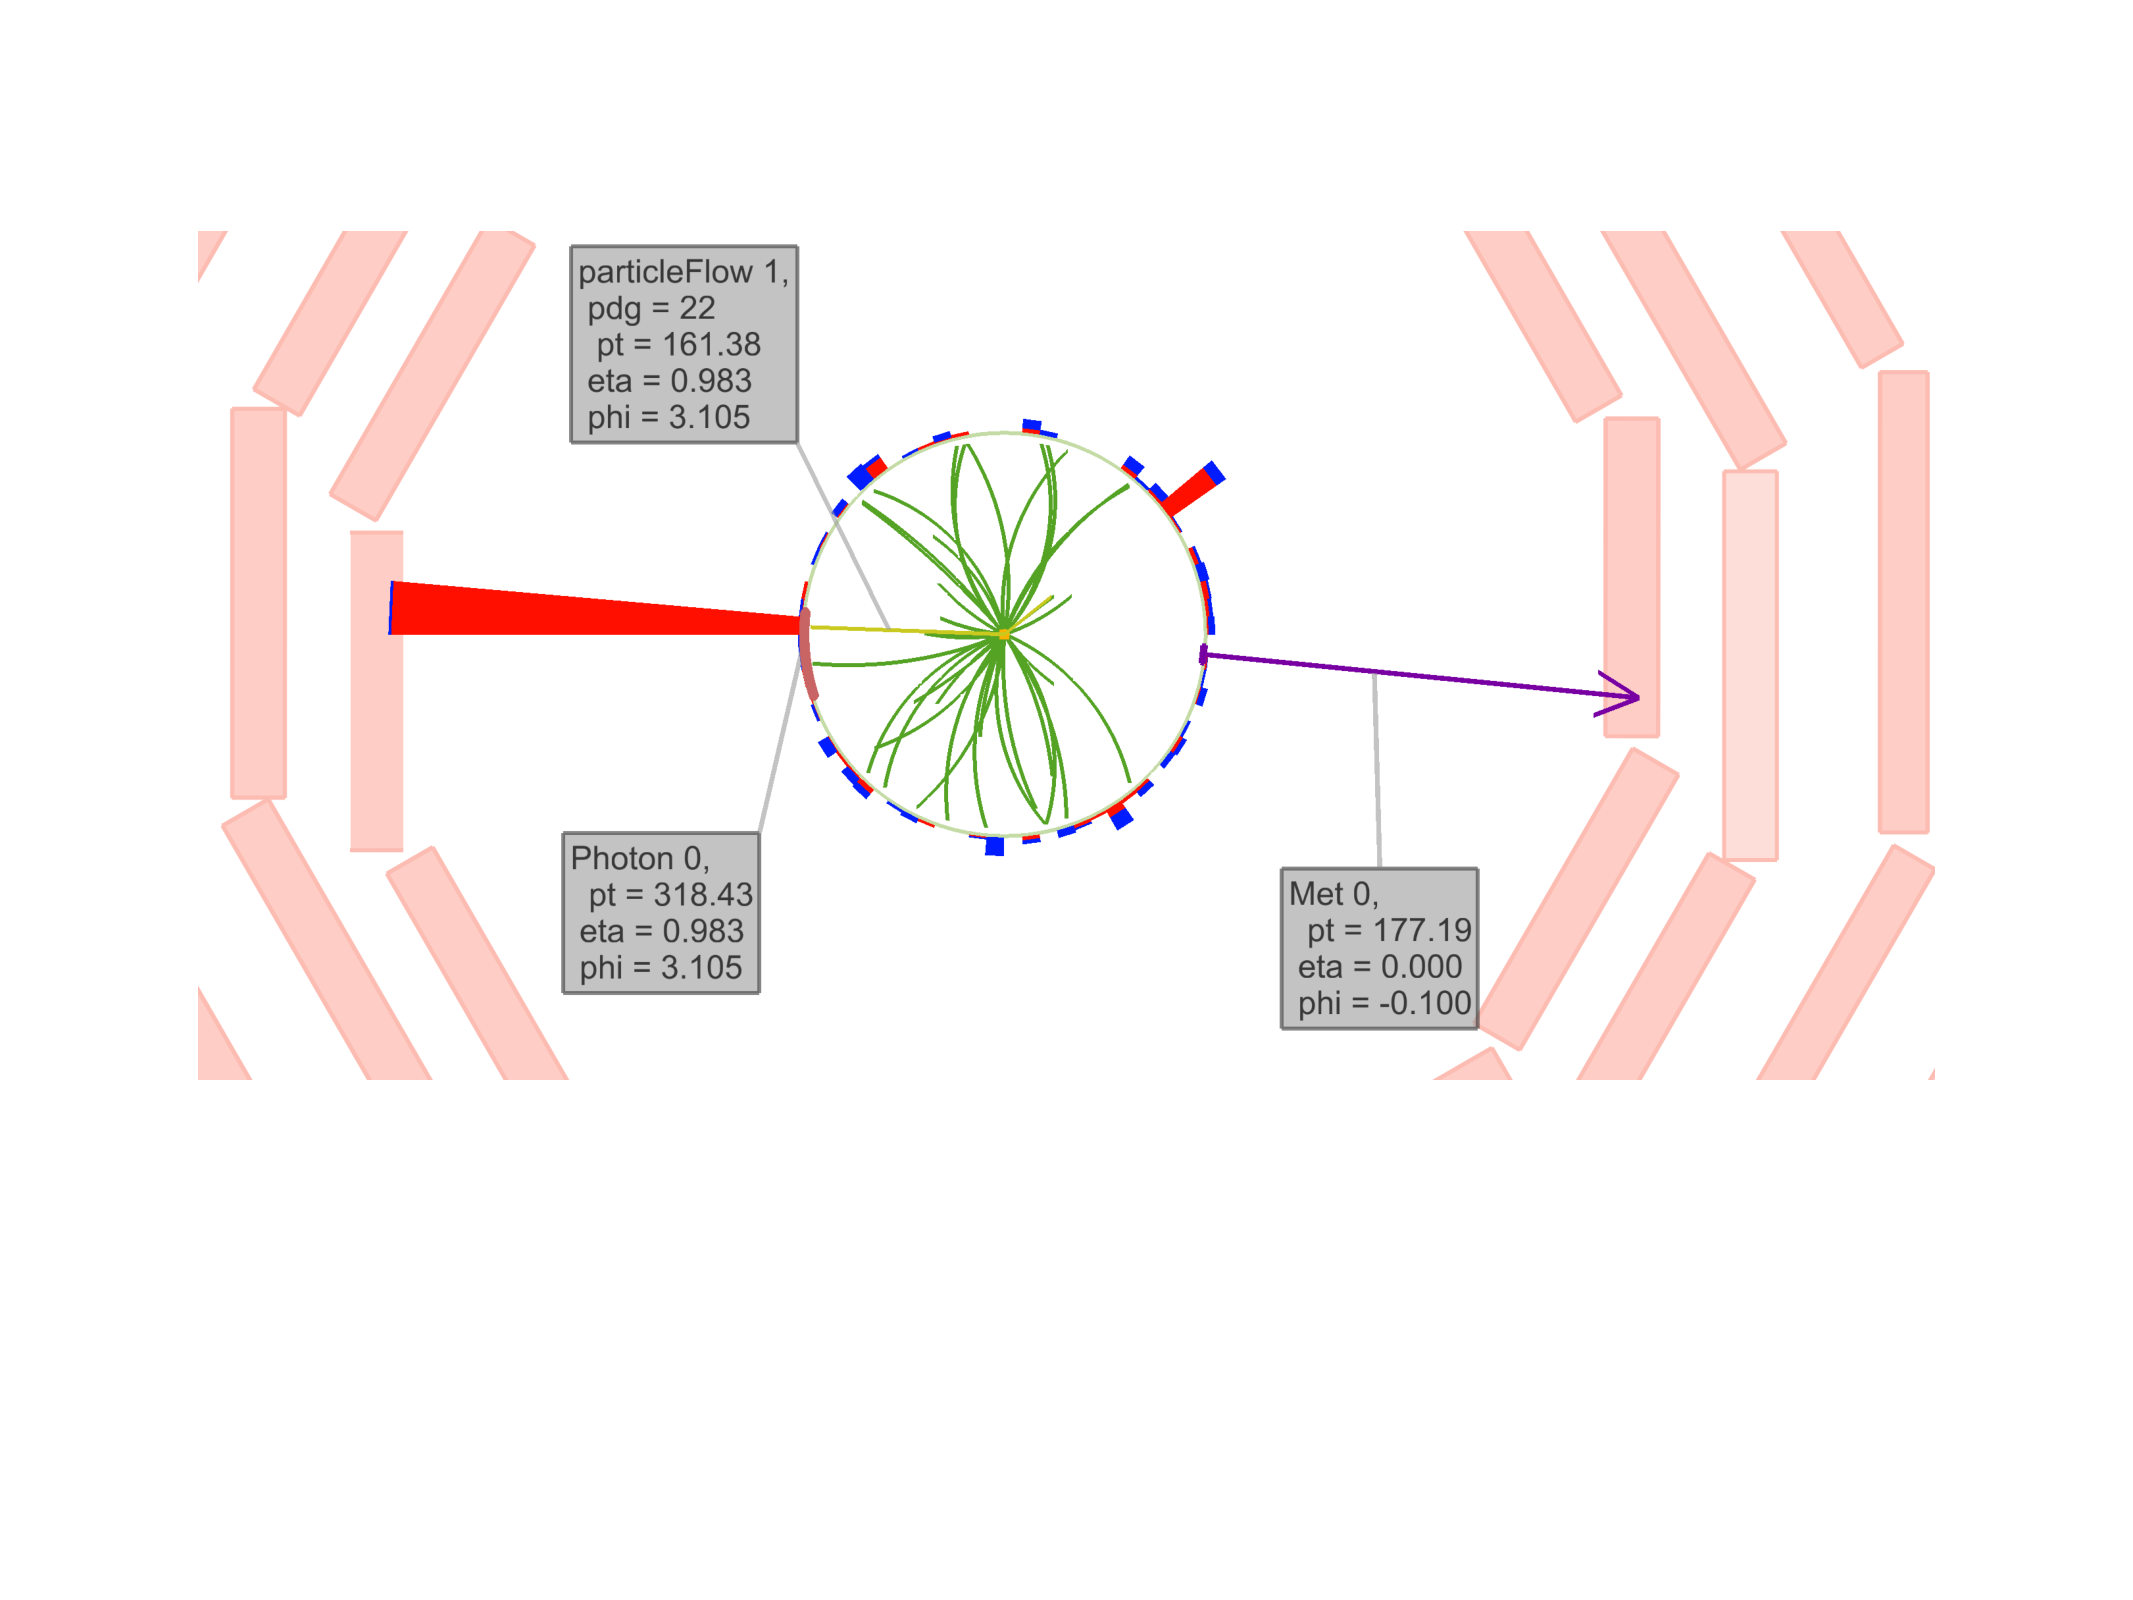
\includegraphics[width=0.6\textwidth]{Reconstruction/Figures/badcorr_evtdisp.pdf}
    \caption{
      An example event where a photon with a wide shower receives a large energy correction.
    }
    \label{fig:badcorr_evtdisp}
  \end{center}
\end{figure}

For the work shown in this thesis, we are only concerned with high-\ET\ photons from the ECAL Barrel that have a supercluster with $\ET > 175\GeV$ and $\abs\eta < 1.4442$. 
To reduce hadron-to-photon misidentification rate, we apply the collection of isolation and shower shape selections in Table~\ref{tab:egid}, which will hereby be referred to as the \egamma\ ID.
To reject electrons from the candidate sample, no electron track seeds in the pixel detector can be associated to the supercluster.
This is known as the pixel seed veto.
To clean the candidate sample from photon objects originating from non-collision sources, we apply the collection of cuts shown in Table~\ref{tab:gsid}, which combined with the pixel seed veto constitutes the \Pgg-specific ID.
The beam halo tagger \emip\ is the total energy deposited in ECAL by a hypothetical beam halo muon that passes through the photon cluster. See Section~\ref{sec:halo} for more detail on beam halo processes. 
The lower bounds on \sieie\ and \sipip\ as well as the requirement on the cluster seed time $\abs\tseed$ are employed to reject spurious photon objects arising from the ``ECAL spikes'' discussed in Section~\ref{sec:spikes}.
%, or anomalous electronic signal induced at the ECAL Barrel photodetectors by nuclear or ionizing interactions in the photocathode.

\begin{table}[htbp]
  \begin{center}
    \begin{tabular}{l | r}
      Variable & Maximum Value \\
      \hline
      $H/E$ &  0.0260 \\ 
      $\sieie$ &  0.01040 \\ 
      $\rho$-corrected \ICHmax\ & 1.146 \\
      $\rho$-corrected \INH\ & $2.792 + 0.0112 \times \ETg + 0.000028 \times \left(\ETg \right)^2$ \\ 
      $\rho$-corrected \Ig\ & $2.176 + 0.0043 \times \ETg$
    \end{tabular}
    \caption{Selections for the \egamma\ portion of the photon ID. Isolation values and \ETg\ are all in units of \GeV.}
    \label{tab:egid}
  \end{center}
\end{table}

\begin{table}[htbp]
  \begin{center}
    \begin{tabular}{l | r}
      Variable & Selection \\
      \hline
      Pixel seed & False \\
      \emip\ & $< 4.9\GeV$ \\
      \sieie\ &  $> 0.001$ \\
      \sipip\ & $> 0.001$ \\
      $\abs\tseed$ & $< 3\ns$ 
    \end{tabular}
    \caption{Selections for the \Pgg-specific portion of the photon ID. \emip\ and $\abs\tseed$ are defined in the text.}
    \label{tab:gsid}
  \end{center}
\end{table}

\subsection{Hadrons}
\label{sec:pf_hadrons}

The last candidates reconstructed in a given block are the charged and neutral hadrons from fragmentation and hadronization, as well as the non-isolated muons and photons produced from their respective decays.

Inside the tracker acceptance of $\abs\eta < 2.5$, all trackless HCAL clusters are reconstructed as neutral hadrons while all trackless ECAL clusters are reconstructed as photons.
The preference towards photons is motivated because photons carry 25\% of the jet energy and neutral hadrons do not interact strongly with the ECAL.
Conversely, outside of the tracker acceptance, it is no longer possible to distinguish charged and neutral hadrons, so any ECAL clusters linked to HCAL clusters are assumed to arise from unidentified charged hadrons.
Thus, only unlinked ECAL clusters are reconstructed as photons and linked ECAL and HCAL clusters are reconstructed as neutral hadrons.

Afterwards, the only remaining PF elements are HCAL clusters linked to one or more tracks and ECAL clusters linked to one of these tracks.
A single charged hadron is constructed for each remaining HCAL cluster, with energy equal to the sum of the ECAL and HCAL clusters and momentum equal to the sum of the individual track momenta.

If the energy of the charged hadron exceeds its momentum by an amount larger than the calometric energy resolution, neutral hadrons and photons are added.
For excesses greater than 500\MeV, a photon with energy equal to the excess is created.
If this photon cannont explain the entire excess, e.g. the excess is larger than the ECAL energy by at least 1\GeV, the remainder is indentified as a neutral hadron. 
After photons and neutral hadrons consume the excess calometric energy, charged hadrons are constructed from the linked tracks with their energy and momentum determined by the track momenta under the charged-pion hypothesis. 

If energy and momentum of the charged hadron are compatible, no neutral particles are identified. A charged hadron candidate is created for each track linked to the HCAL cluster, with momenta determined by a $\chi^2$ fit of the tracker and calorimeter measurements.
This combintation ensures a smooth transition between the tracker-dominated low-enrgy regime and the calorimeter-dominated high-energy regime while always improving the final energy resolution. 

If the momentum of the charged hadron exceeds its energy by three standard deviations, new PF muons are made from any non-isolated global muons failing the cleaning described in Section~\ref{sec:pf_muons} with momentum resolution better than 25\%.
If, after masking the tracks from these muons, the track momentum sum still greatly exceeds the calorimeter energy, all remaining tracks with a \pt\ uncertainty greater than 1\GeV are identified, sorted in decreasing order of this uncertainty, and sequentially masked until no such tracks remain or the momentum excess disappears, whichever comes first. 
At this point, the HCAL cluster is reconstructed according to one of the procedures defined in the preceding paragraphs.

When three or more charged particle candidates are linked to a secondary vertex identified as described in Section~\ref{sec:pf_csv}, a single primary charged hadron with energy equal to the sum of their energies replaces them in the reconstructed particle list.
If an incoming track is associated with the vertex, it determines the direction of the primary charged hadron, which is otherwise determined by the vectorial sum of momenta of the secondary particles.
If the momentum of the incoming track is well measured, the energy of undetected secondary particles is estimated and added to the energy of the primary charged particle.

\subsection{Jets}
\label{sec:pf_jets}

As discussed in Section~\ref{sec:lhc_pheno}, jets are produced during the fragmentation and hadronization of colored particles produced in the hard scattering.
After all PF candidates have been identified, a sequential recombination algorithm is used in an attempt to cluster these jets.
Given an object $i$ in the event $E$, we define the distance to the beam and the distance to another object $j$ to be
\begin{equation}
  \begin{matrix}[l | r]
    \displaystyle
    d_{iB} = \left(\pt^i\right)^{2q} &
    d_{ij} = \min \left\{\left(\pt^i\right)^{2q}, \left(\pt^j\right)^{2q} \right\} \dfrac{\left(\dR_{ij}\right)^2}{R^2} ,
  \end{matrix}
\end{equation}
respectively, where $q$ and $R$ are tunable parameters and $\dR_{ij}$ is the angular distance between the two particles.
The distance parameter $R$ is an appromixate measure of the cone size \dR\ of the jet, while the power of the energy scale $q$ defines the relationship between the relationship between the momentum and angular factors.
Jets clustered with $q = -1$ are referred to as anti-\kt\ jets, those with $q = 0$ as Cambridge-Aachen jets, and those with $q = 1$ as \kt\ jets.  
Negative values of $q$ force the clustering of circular jets around hard seeds ensuring that the resulting jet boundaries are resilient with respect to soft radiation.
Within CMS, anti-\kt\ jets with $R = 0.4$ are used to cluster the parton shower from single partons.

The implementation in the FastJet library reduces the computational complexity of clustering from $\mathcal{O}(N^2)$ to $\mathcal{O}(N \log N)$ for jets with hundreds or thousands of constituent particles.
First, the two objects $i$ and $j$ with the smallest distance $d_{ij}$ between them are found. 
If $d_{ij}$ is less than both $d_{iB}$ and $d_{jB}$, they are removed from $E$ and a single object $k$ with four-momentum $p_\mu^k = p_\mu^i + p_\mu^j$ which is added in their place. 
Otherwise if $d_{iB} < d_{jB}$, object $i$ is removed from $E$ and added to the set of jet candidates $J$ while object $j$ is kept, and vice versa if $d_{jB} < d_{iB}$.
This procedure continues until all objects are removed from $E$ and $J$ contains all possible jet candidates.

\subsection{Missing Tranverse Energy}
\label{sec:pf_met}

The production of neutrinos and dark matter candidates produces a momentum imbalance in the transverse plane.
The missing transverse momentum \ptvecmiss\ is defined as the negative vectorial sum of all the PF candidates in the event $E$ such that
\begin{equation}
  \ptvecmiss = - \sum_{i\in E} \Big( \hat x \cdot \pt^i \cos \phi + \hat y \cdot \pt^i \sin \phi \Big),
\end{equation}
and its magnitude is the missing transverse energy $\met = \abs\ptvecmiss$.
In a perfectly reconstructed event, non-zero \met\ implies the presence of neutrinos or DM candidates; however, the failure to properly reconstruct energy deposits or the reconstruction of PF candidates with incorrect energy results in events with large amount of fake \met.

One last cleaning of the PF candidates is conducted in an attempt to fix these events.
To remove muons from cosmic rays, muon candidates with trajectories more than 1\cm away from the beam axis are removed if the measured \met\ is consequently reduced by half.
For muons with $\pt > 20\GeV$, the choice of subdetector used to estimate momemtum is reviewed and the smallest available estimate used if it reduces the measured \met\ by half.
Additionally, the assignment of charged hadrons and neutral hadrons is reconsidered to ensure a charged hadron is not reconstructed as a muon and neutral hadron and vice versa.

Fake \met\ can persist in an event even after the final cleaning of PF candidates.
At this point, events are checked against a known set of filters identifying possible sources of fake \met\ not captured by the PF algorithm.
One set of filters is the HCAL and ECAL filters that identify events with calorimeter clusters caused by noise from the shape and timing of the energy distribution.
Another such filter is the beam halo filter that identifies energy deposits from muons produced from interactions between the beam and the machine that travel parallel to the beam. These muons are identified by their localization in $\phi$ and a longitudinal track left in the ECAL endcaps and the CSCs.
Applying these filters removes essentially all remaining events with fake \met\ while rejecting less than 1\% of events with real \met.

\section{Reconstruction Issues}
\label{sec:issues}

The work shown in this thesis focuses on events with a single high-\pt\ photon and large \met.
There are a lot of reconstruction issues specific to this final state as photons are relatively easy to fake through other processes that result in a large amount of \met.
This section describes the three main sources of fake photons and fake \met encountered during this analysis.

\subsection{ECAL gain-switch effect}
\label{sec:gainswitch}

\begin{figure}[htbp]
  \centering
  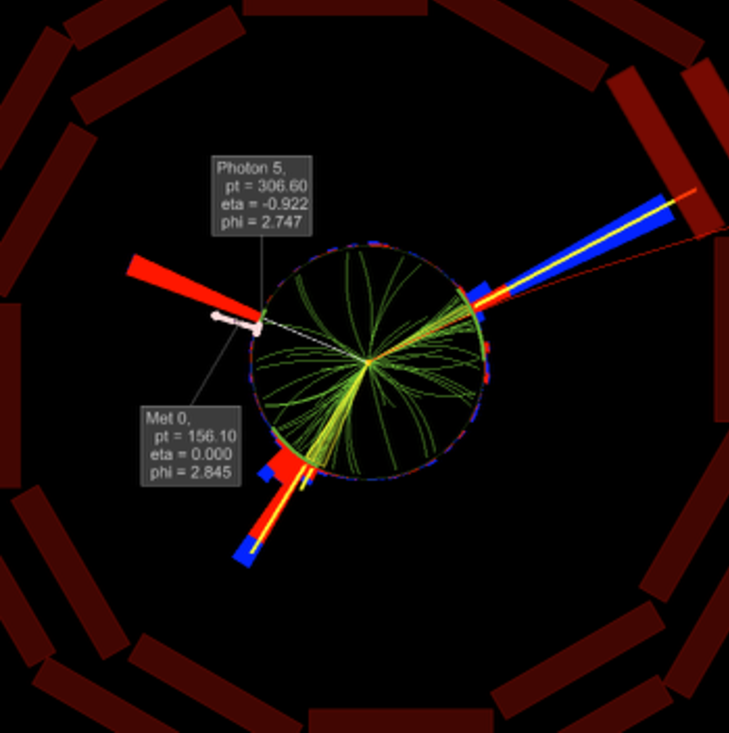
\includegraphics[width=0.48\linewidth]{Reconstruction/Figures/gsfix/evdisp_before.pdf}
  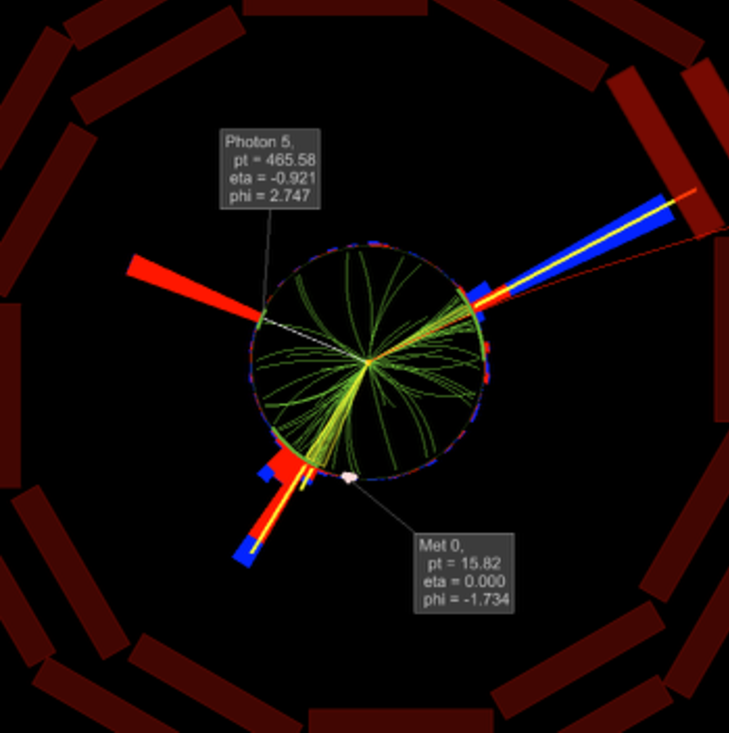
\includegraphics[width=0.48\linewidth]{Reconstruction/Figures/gsfix/evdisp_after.pdf}
  \caption{
    Two event displays comparing the same event, reconstructed without (left) and with (right) the fix for ECAL gain-switch effect.
  }
  \label{fig:eventdisplay_gsfix}
\end{figure}

The ``multi-fit'' algorithm for ECAL hit reconstruction was found to have an unexpected behavior when there is a large energy deposit onto a single ECAL crystal, such that the electronic signal converted at the frontend electronics is sourced partially from channels of the preamplifier with lower gains (6 or 1) than the default (12) channel. 
In the most dramatic cases, pulse misreconstruction would result in underestimation by hundreds of \GeV of photon \pt. 
This effect is mitigated in the reprocessed data set used for this analysis by identifying ECAL clusters whose seed crystal hit had a switch of gains, and performing an alternative pulse reconstruction when possible.

\begin{figure}[htbp]
  \centering
  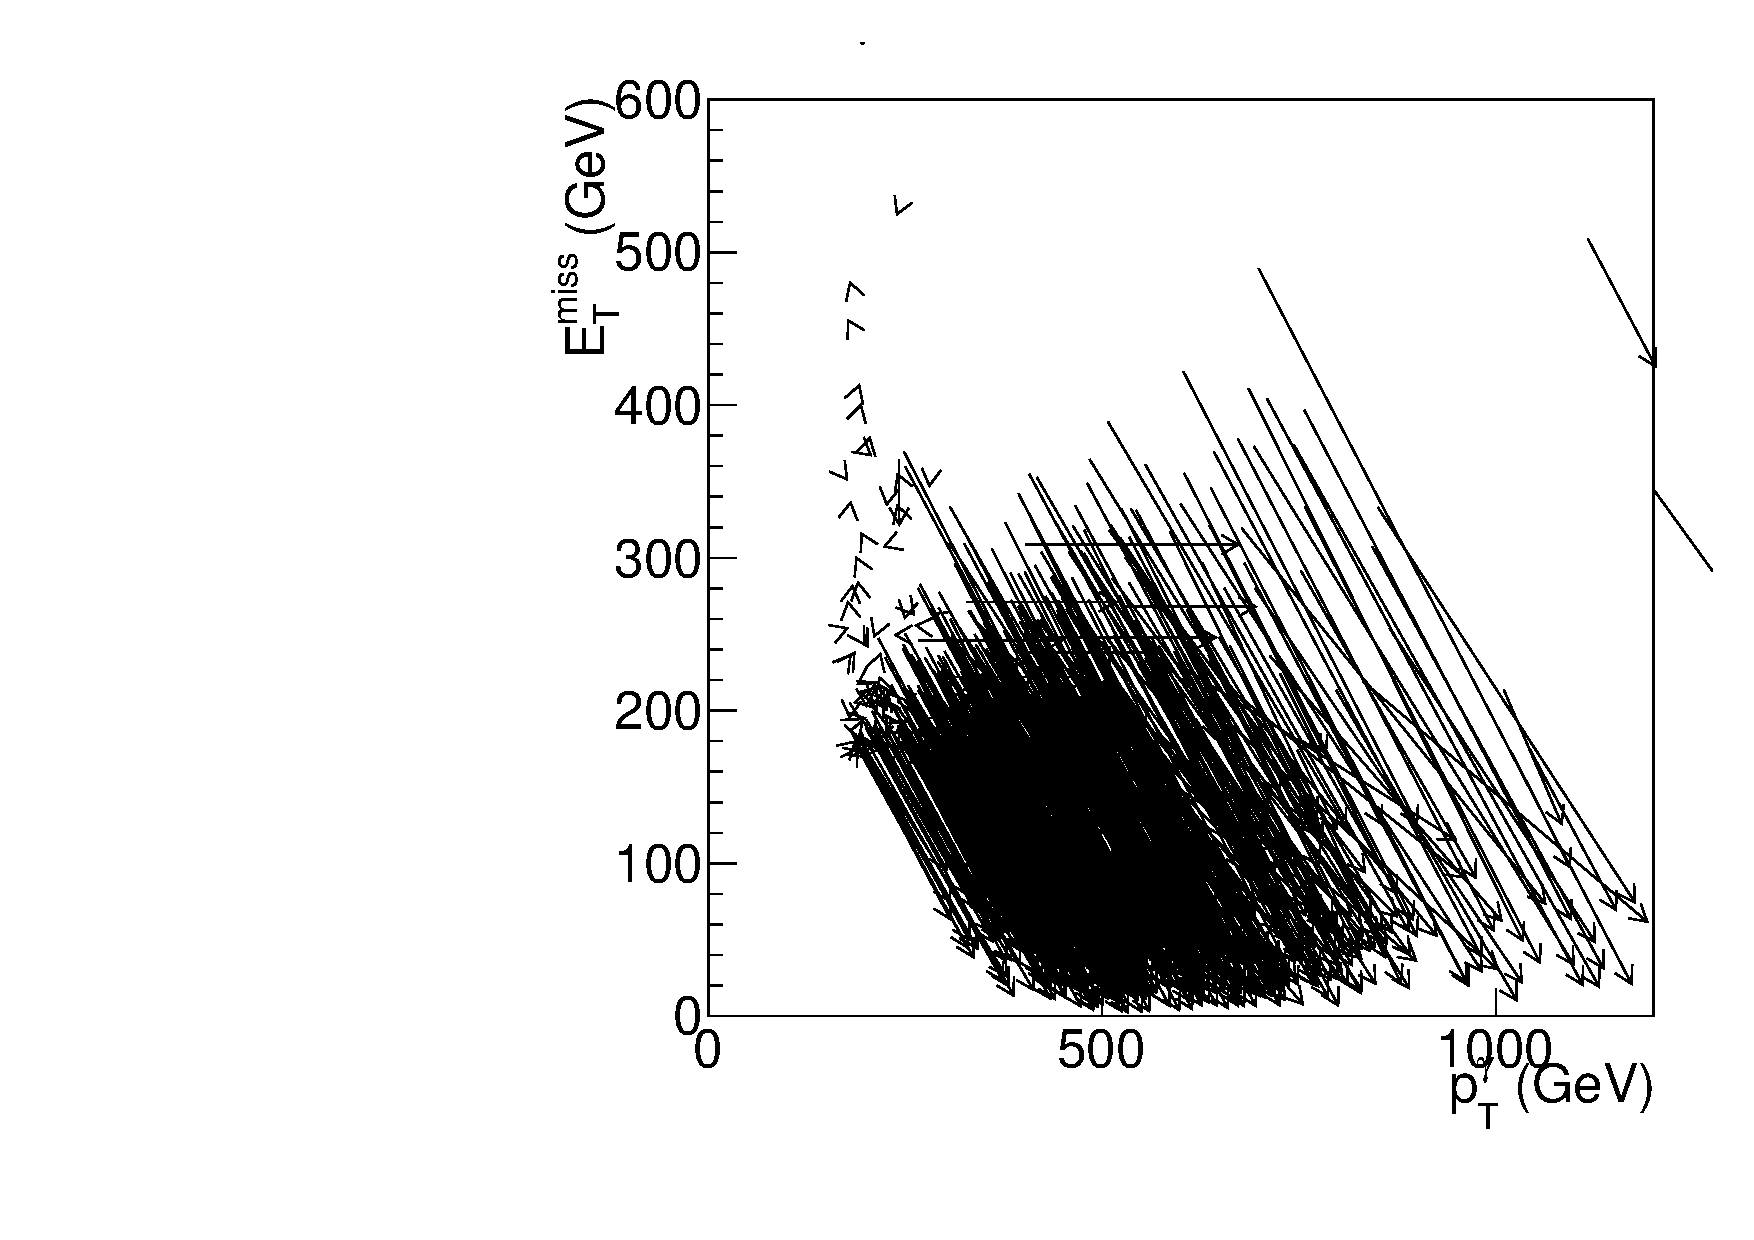
\includegraphics[width=0.48\linewidth]{Reconstruction/Figures/gsfix/movements.pdf}
  \caption{
    The change in reconstructed photon \pt\ and \met\ for events in the bin $\dphigmet < 0.05$ of the distribution in Figure~\ref{fig:dphigmet_beforegsfix}. 
    Each arrow represents a single event, the the tail (head) of the arrow corresponding to (\ETg, \met) coordinates in the datasets without (with) the fix for the gain-switch problem.
  }
  \label{fig:ptshift_gsfix}
\end{figure}

The gain-switch problem affected the analyses documented in this thesis, since large underestimation of the energy of a photon in an otherwise typical \gj\ event would introduce large missing transverse momentum to the event, typical collinear to the affected photon. 
Figures~\ref{fig:eventdisplay_gsfix} and~\ref{fig:ptshift_gsfix} are the visualization of how the new dataset changes the reconstructed photon energy and \met.

\subsection{Beam Halo Phenomenology}
\label{sec:halo}

Bremsstrahlung photons emitted by beam halo muons in the ECAL volume generate a physical EM shower in the ECAL crystals. 
Large deposits energy are rare, but the rate of beam halo penetration during the 2016 run was substantial. 
The characteristic features of a shower caused by a halo particle include coincident hits in the barrel muon system and a ``trail'' of low-energy clusters in ECAL along the particle trajectory. 
The beam halo MET filter described in Section~\ref{sec:pf_met} exploits the former, while the \emip\ variable described in Section~\ref{sec:pf_photons} captures the latter.

\begin{figure}[tbp]
  \begin{center}
    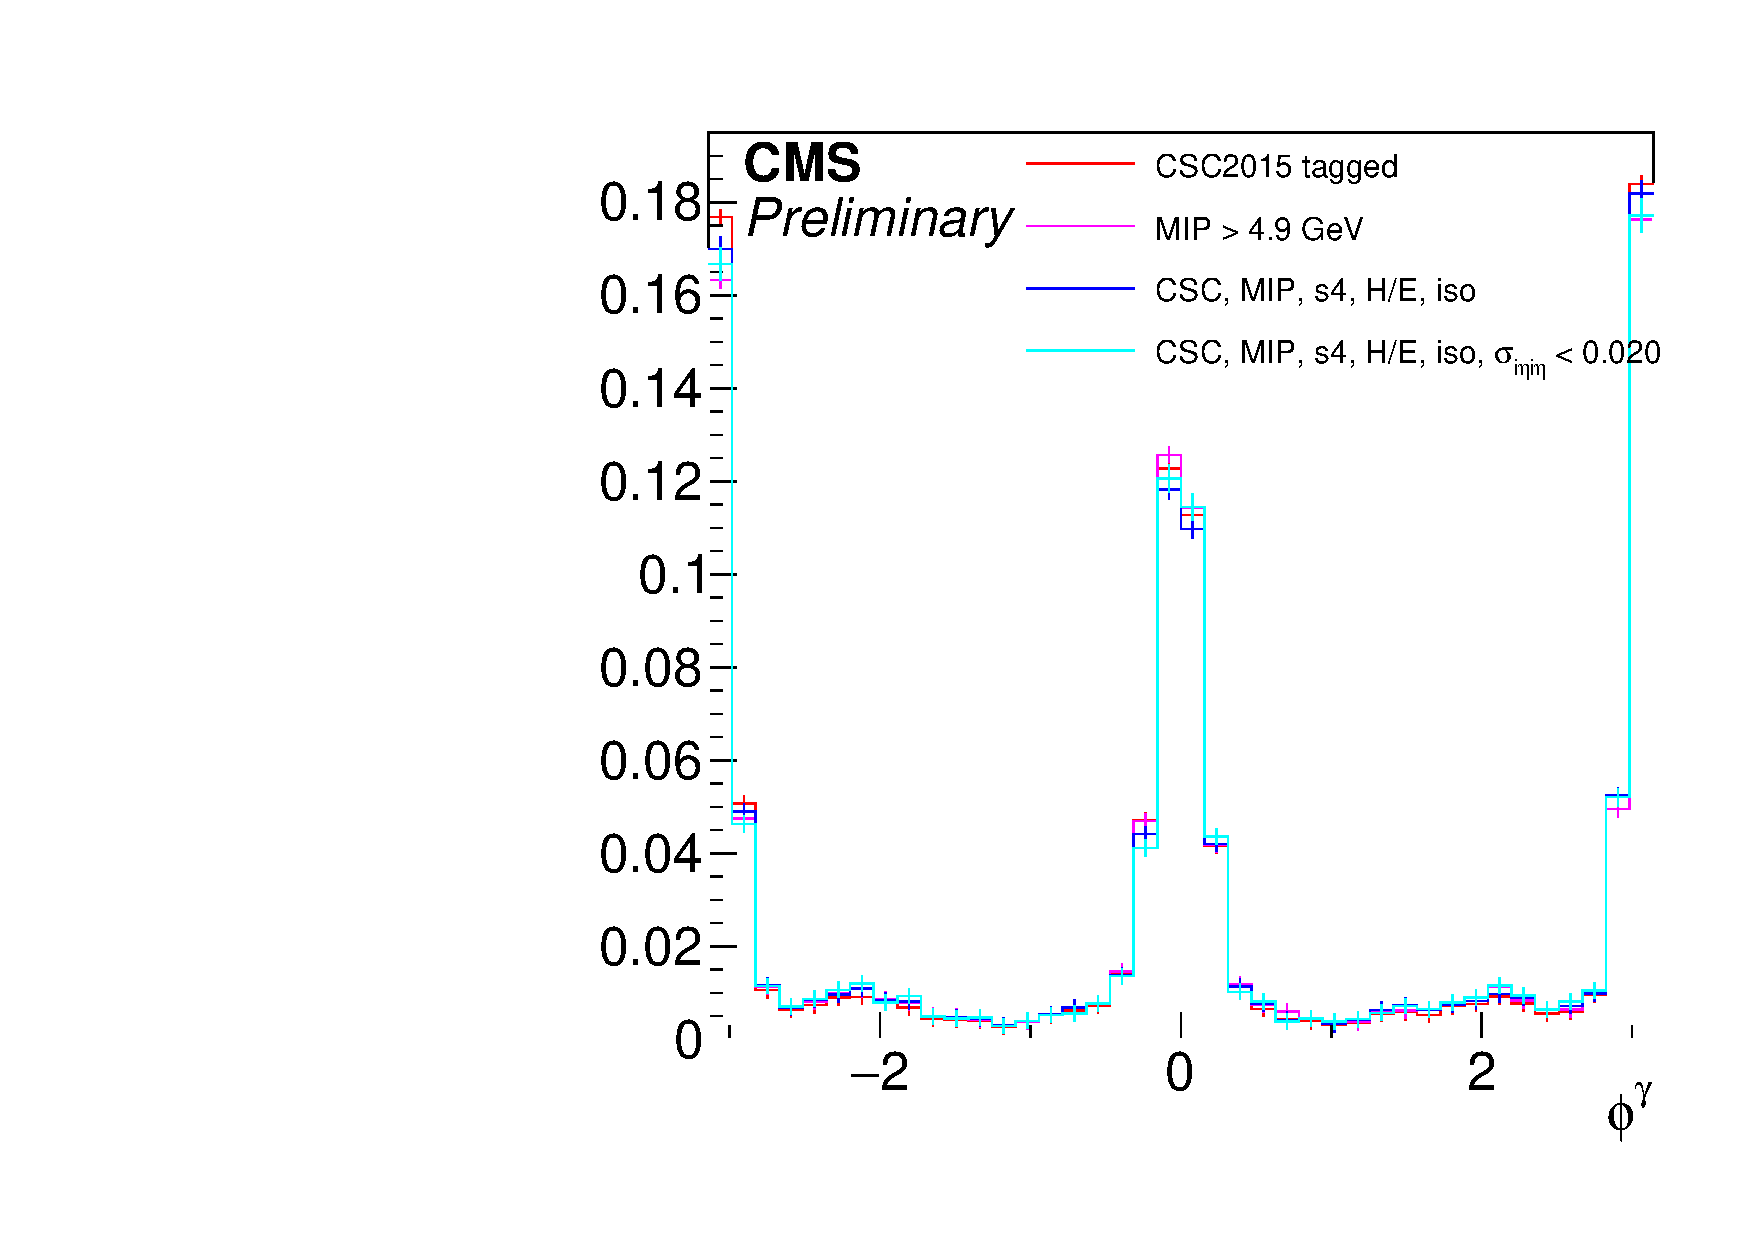
\includegraphics[width=0.6\textwidth]{Reconstruction/Figures/halo/halophi.pdf}
    \caption{
      The \phig\ distribution of the halo-like showers, tagged in multiple ways. 
      Histograms are normalized to unity.
      The cyan histogram is the \phig\ distribution after applying photon identification selections except for the shower shape. 
      It can be seen that the \phig\ distribution is highly stable against the listed identification selections.
    }
    \label{fig:halophi}
  \end{center}
\end{figure}

\begin{figure}[tbp]
  \begin{center}
    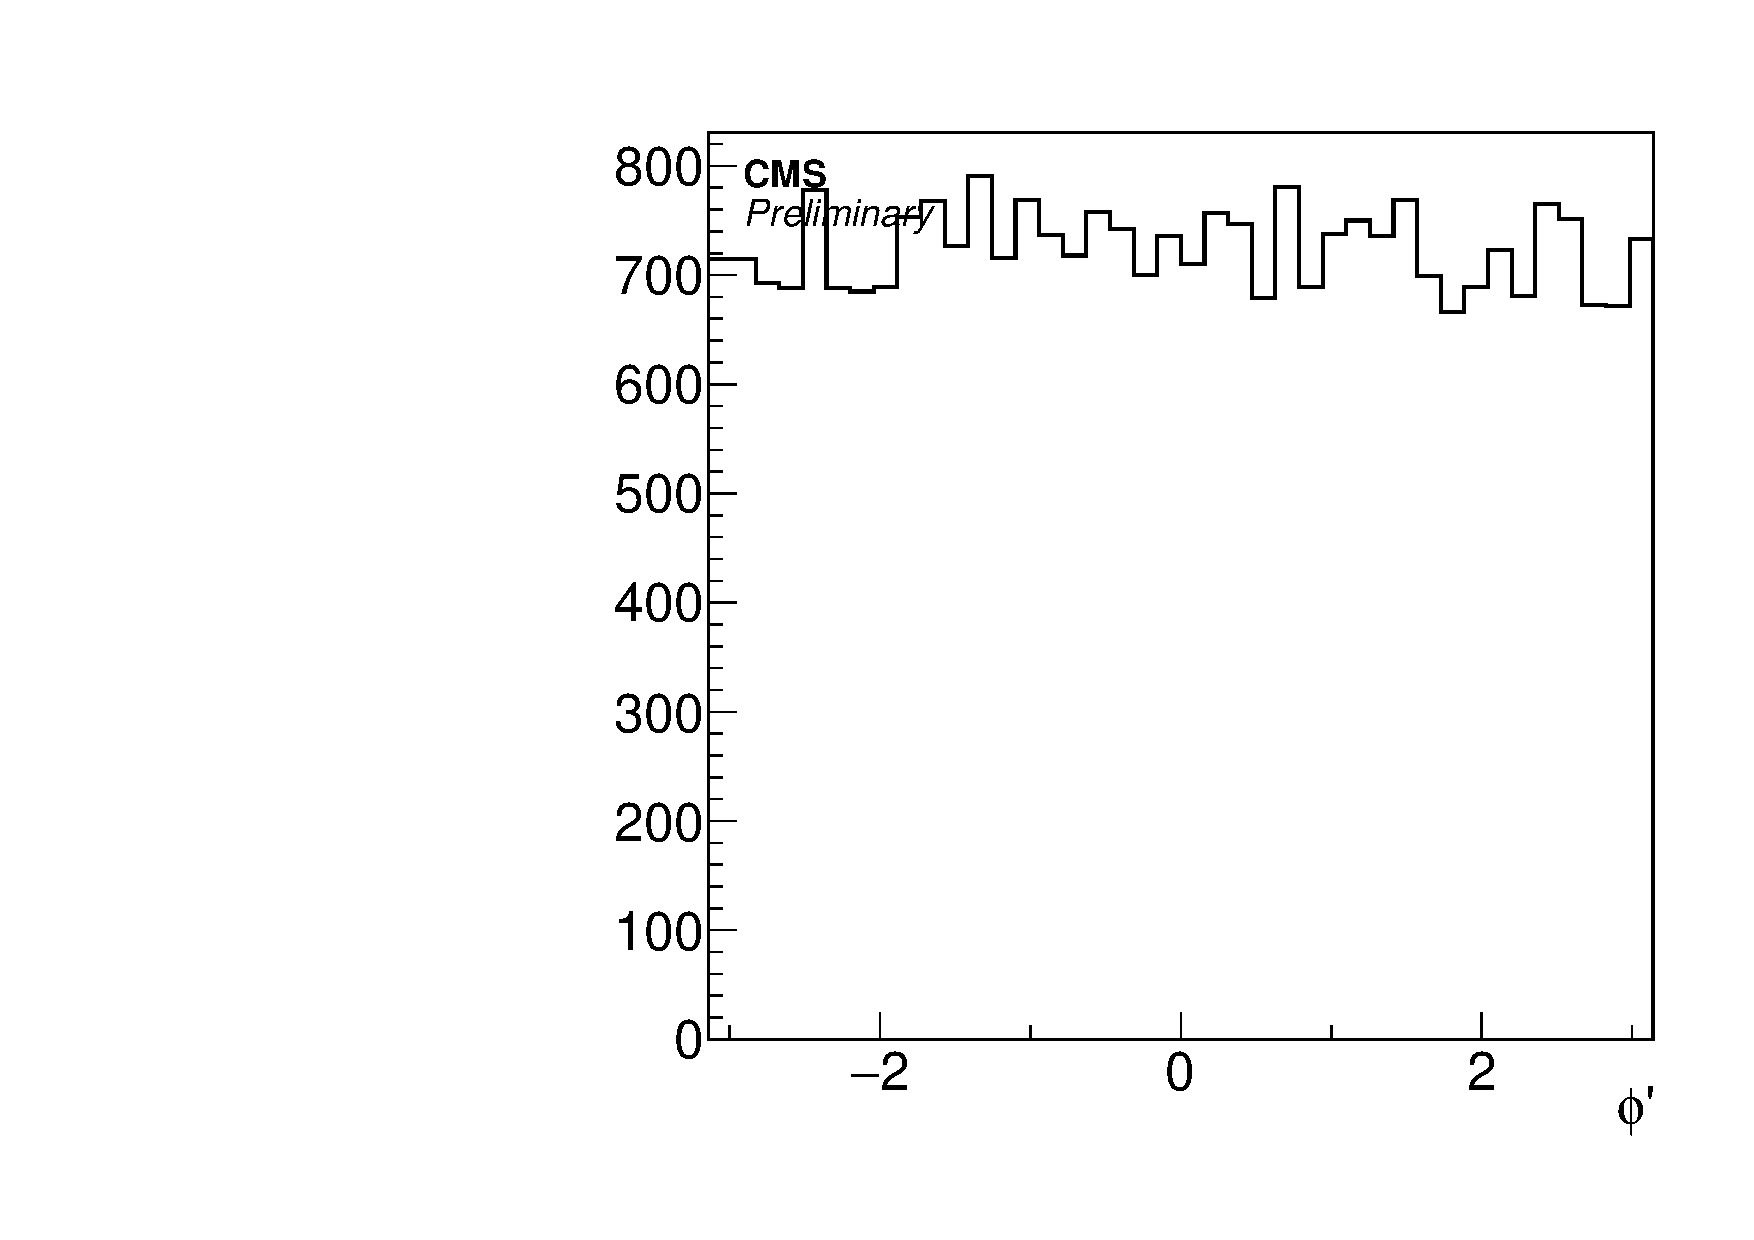
\includegraphics[width=0.6\textwidth]{Reconstruction/Figures/halo/bkgphi.pdf}
    \caption{
      The \phig\ distribution from \zinvg\ MC simulation.
    }
    \label{fig:bkgphi}
  \end{center}
\end{figure}

Because beam halo particles are produced through complex LHC machine effects, it is natural that the observed distribution of the halo showers is not
symmetric in the azimuthal angle in the detector coordinates.
Figure~\ref{fig:halophi} is a \phig\ distribution of the halo showers obtained from the Single Photon data set, requiring $\met > 140\GeV$. 
Here, halo showers are defined as those that fail the MIP-tagging and in the event tagged by the CSC beam halo tagger. 
On the other hand reconstructed shower from all other sources are symmetric in \phig\, as demonstrated in Fig.~\ref{fig:bkgphi}. 

\begin{figure}[tbp]
  \begin{center}
    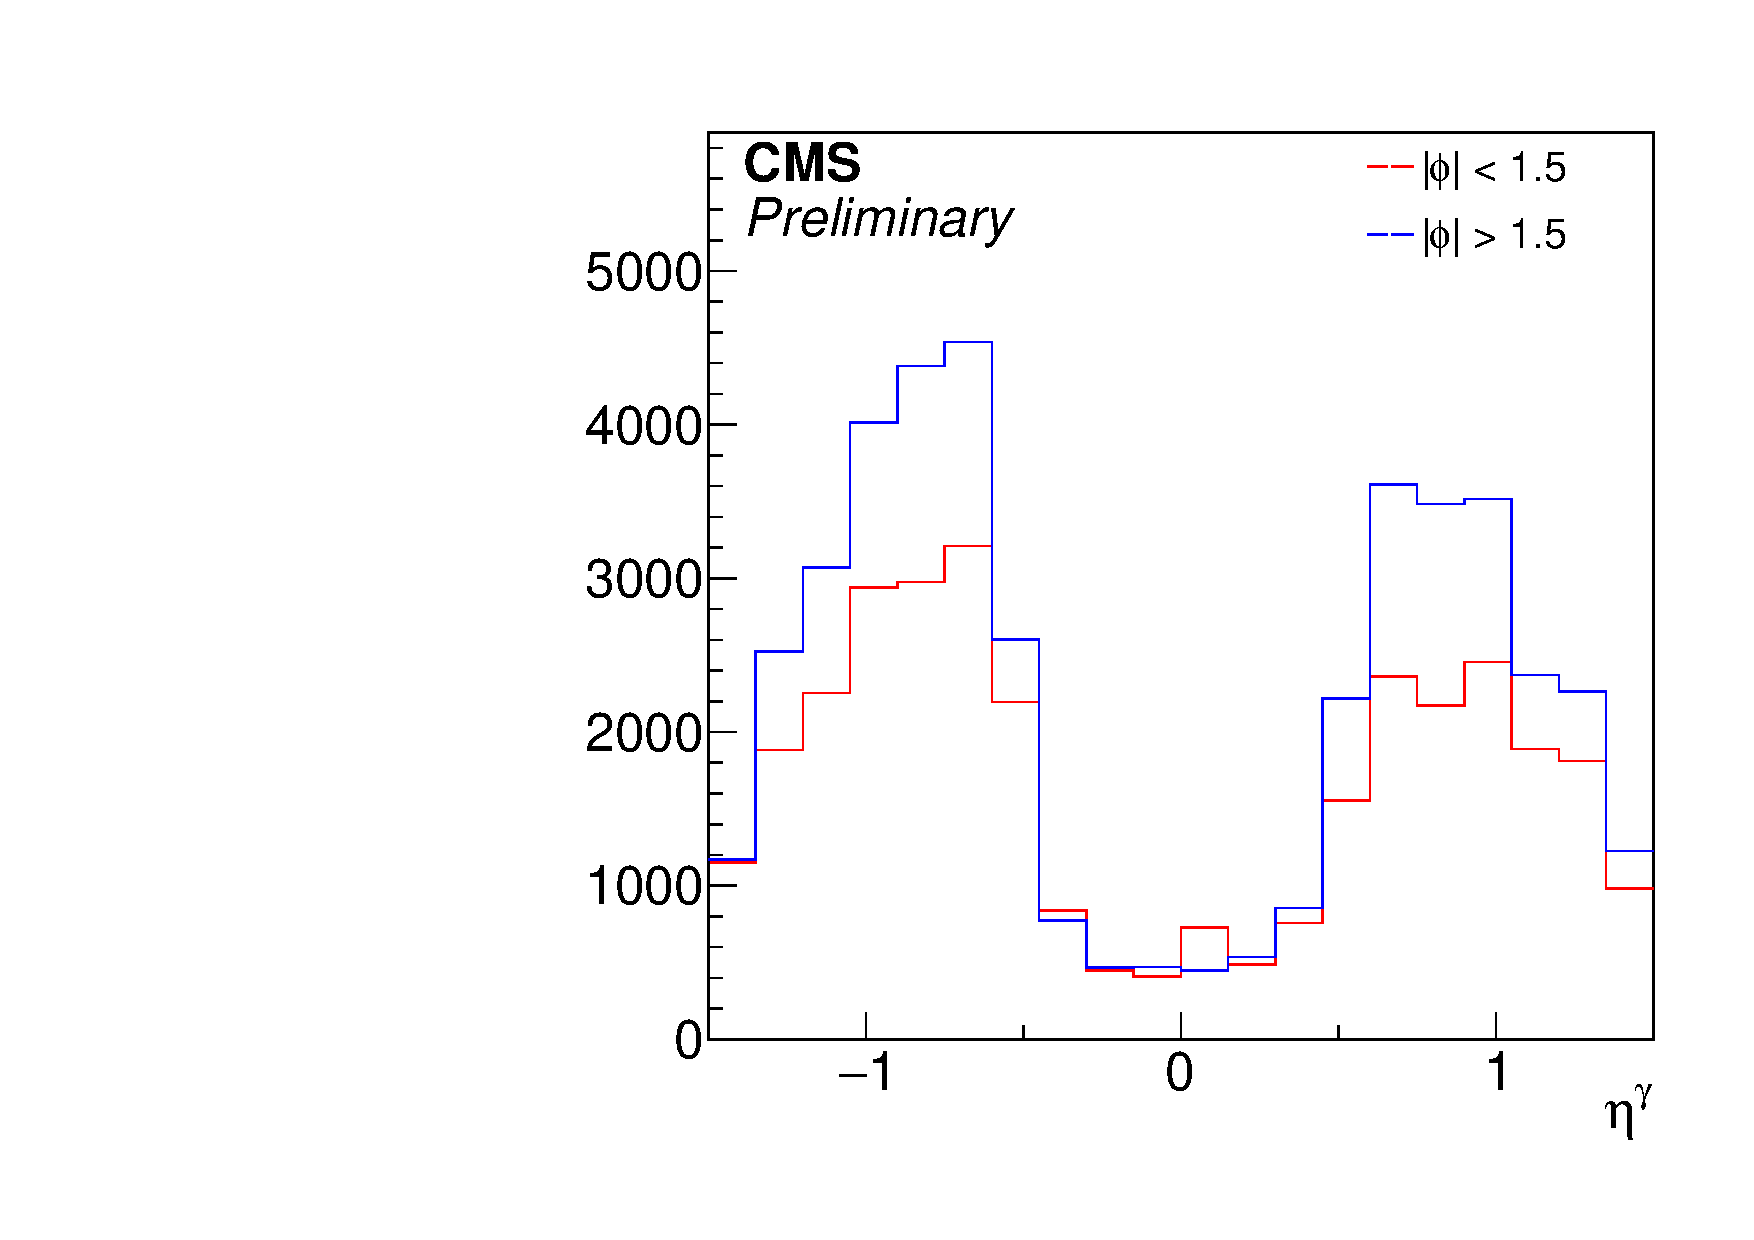
\includegraphics[width=0.3\textwidth]{Reconstruction/Figures/halo/halo_eta.pdf}
    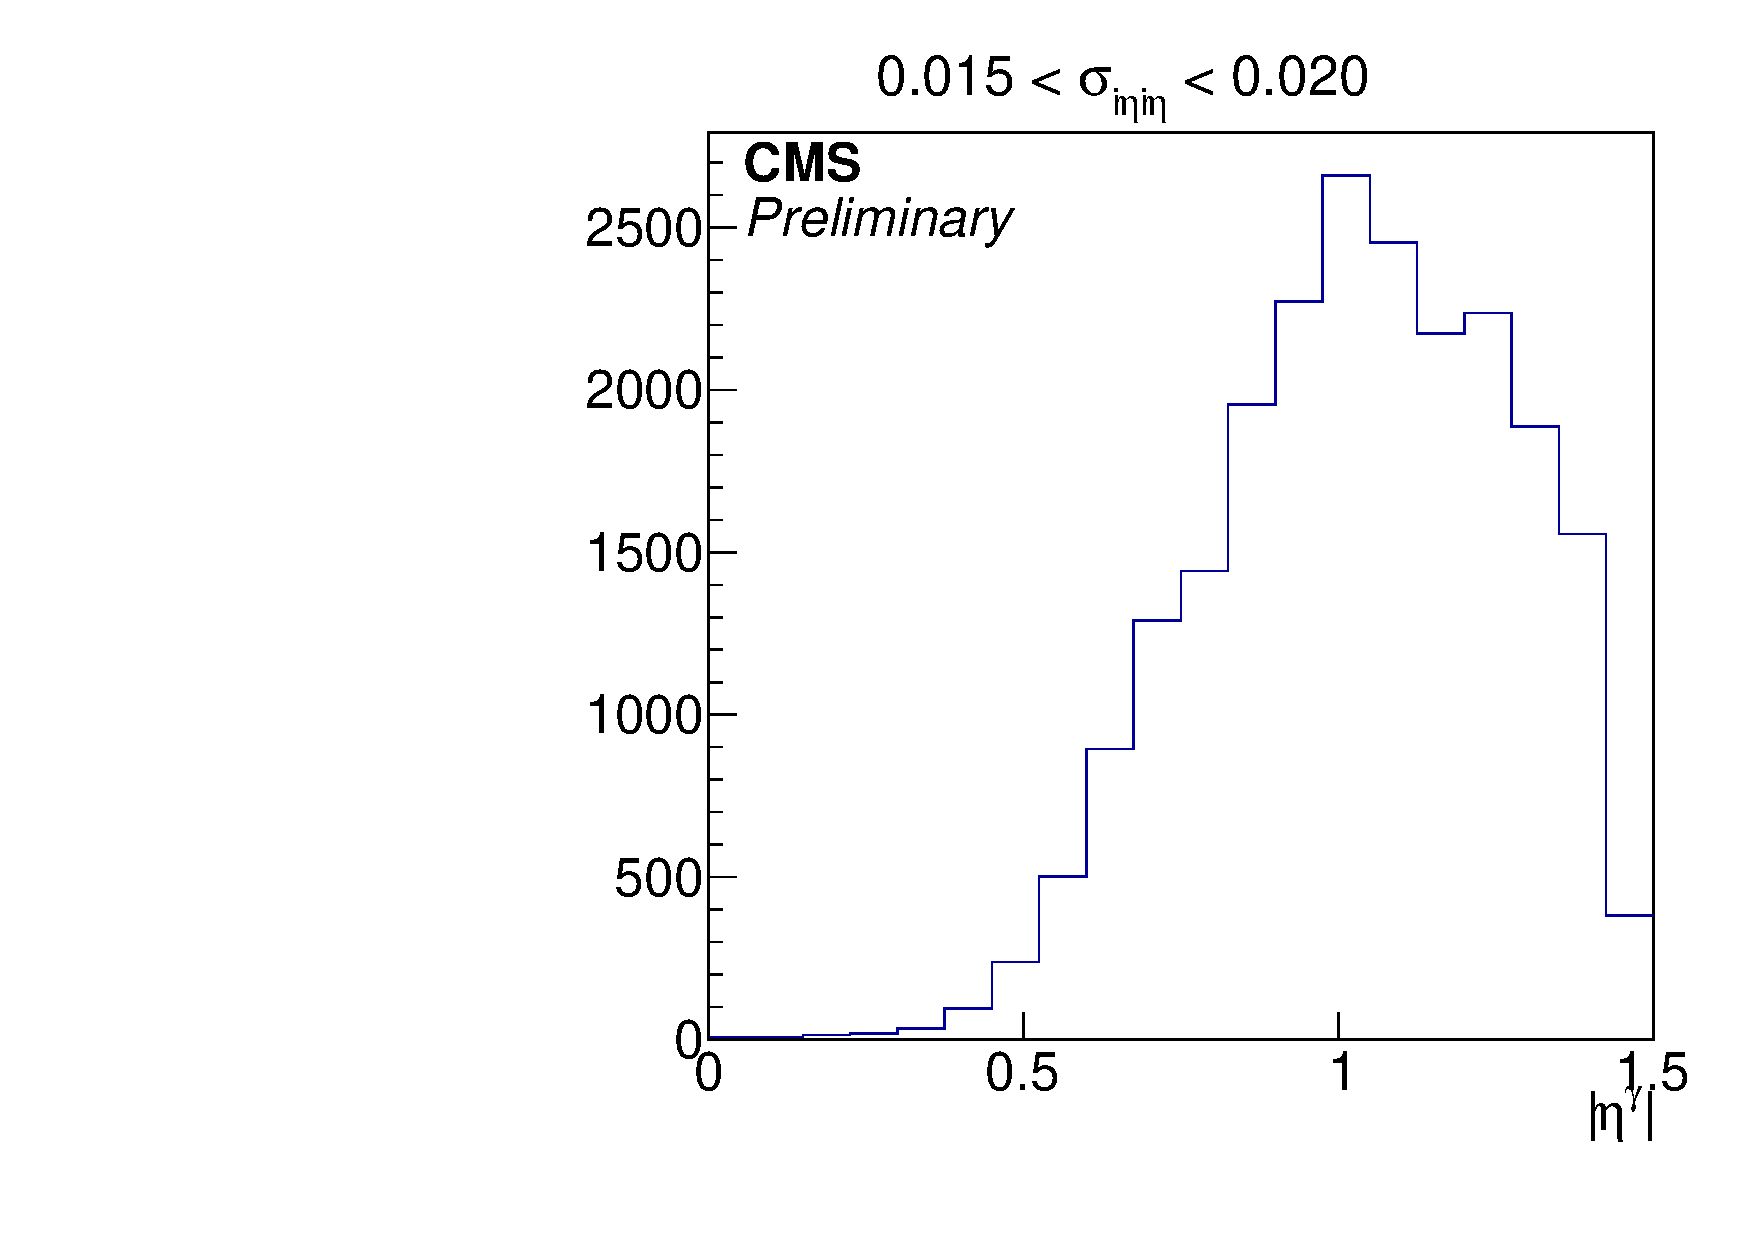
\includegraphics[width=0.3\textwidth]{Reconstruction/Figures/halo/halo_shape_etalow.pdf}
    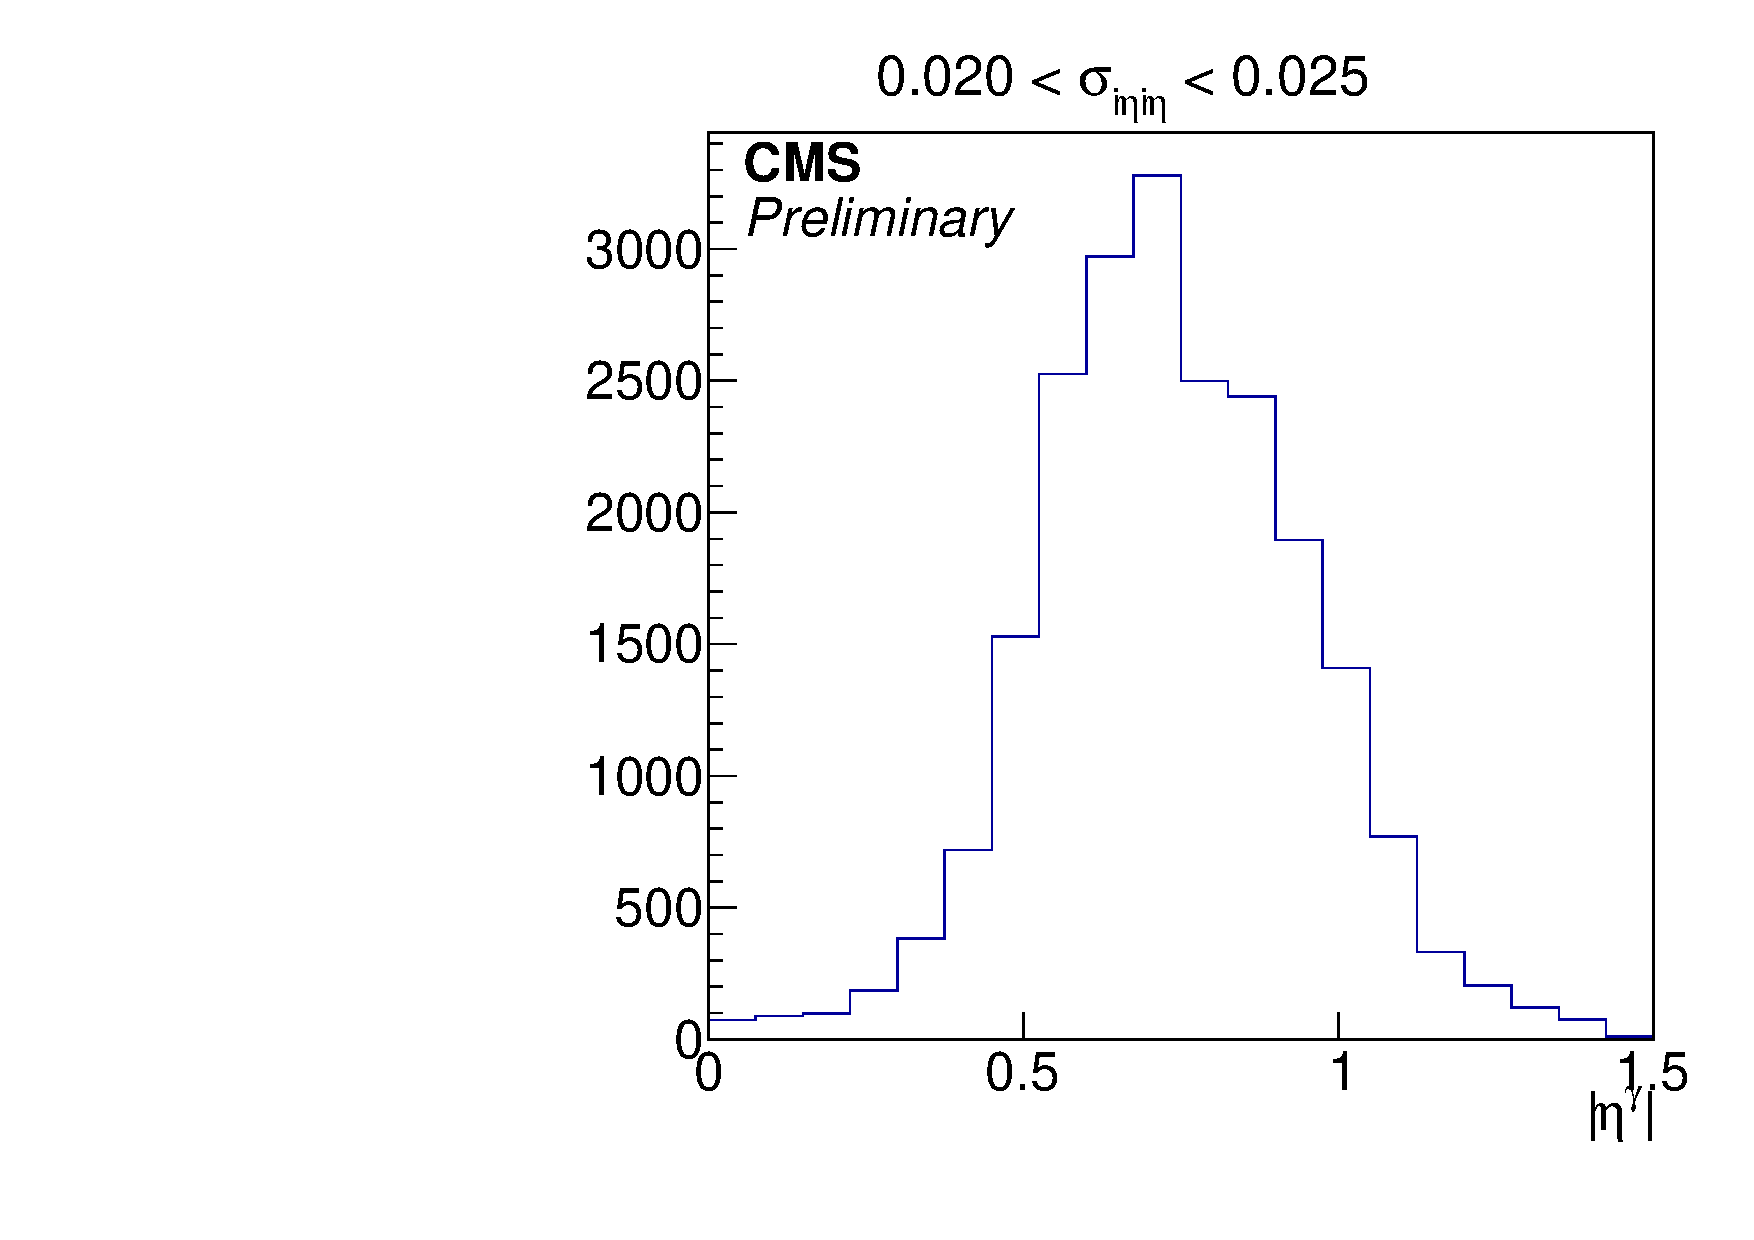
\includegraphics[width=0.3\textwidth]{Reconstruction/Figures/halo/halo_shape_etahigh.pdf}
    \caption{
      Left: $\eta$ distribution of the halo-like showers with $|\phi| < \pi/2$ and $|\phi| > \pi/2$.
      Middle and right: shift in the $\eta$ distribution of the halo-like showers with respect to the requirement on \sieie.
    }
    \label{fig:halo_eta}
  \end{center}
\end{figure}

For the distribution of Fig.~\ref{fig:halophi} to be a valid template for halo showers, it must be first confirmed that its shape is invariant under photon selection requirements. 
However, further study of the \phig\ distribution of the halo showers indicates that the relative strength of the two prominent peaks in the distribution may change under the \sieie\ selection requirement.  
To explain this phenomenon, one needs to look at the the \etag\ distribution of the shower populations near $\phig \sim 0$ and $\phig \sim \pi$, shown in the top portion of Figure~\ref{fig:halo_eta}. 
Meanwhile, halo showers tend to have narrower shape in the $\eta$ direction when occurring at high $\eta$, due to the projective geometry of the ECAL crystals, visible in the bottom portion of Figure~\ref{fig:halo_eta} bottom). 
Combining the two observations, the conclusion is that the stringent requirement on the narrowness of the shower in the photon selection will preferentially reduce the $\phi \sim 0$ population.

\begin{figure}[tbp]
  \begin{center}
    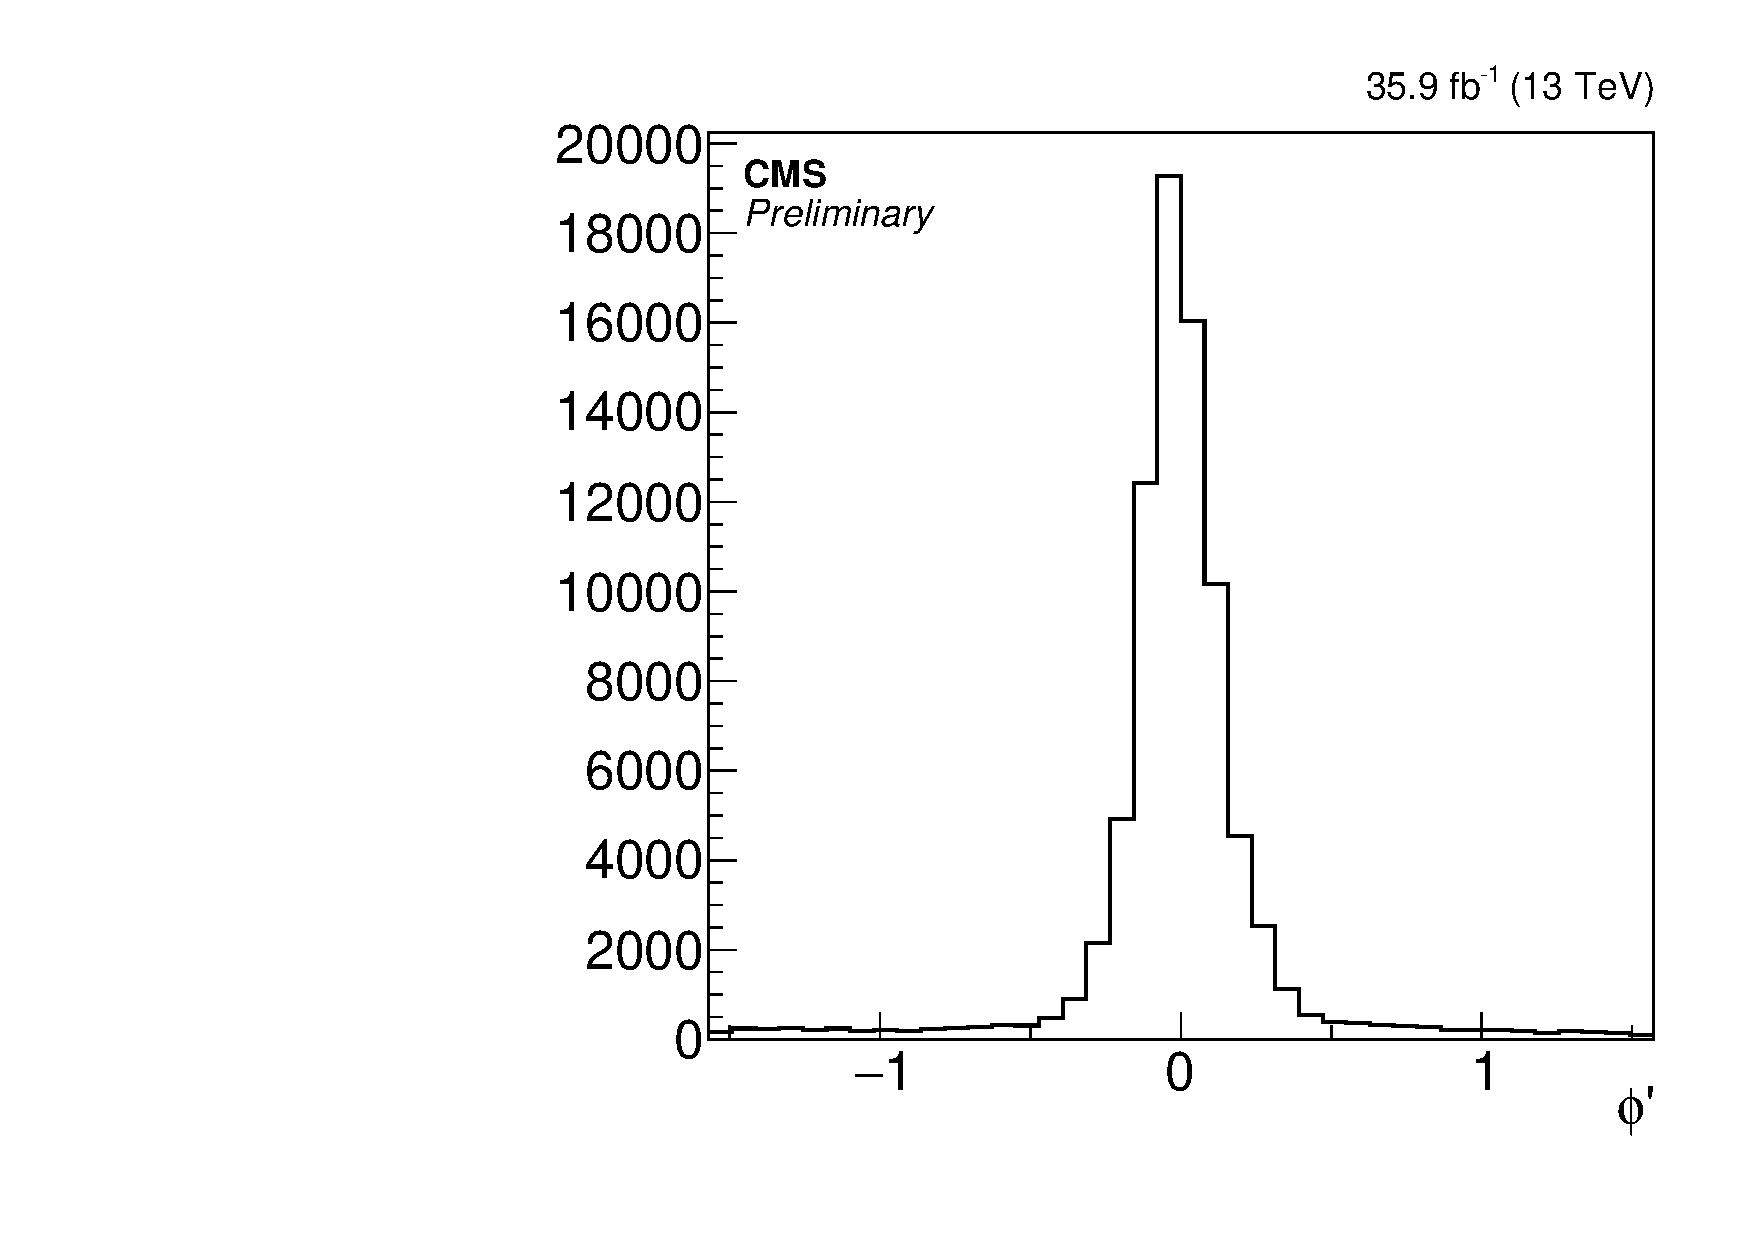
\includegraphics[width=0.45\textwidth]{Reconstruction/Figures/halo/haloPhiFolded.pdf}
    \caption{
      Folded $\phi'$ distribution of the halo sample.
    }
    \label{fig:halo_template}
  \end{center}
\end{figure}

Nevertheless, the invariance under photon selection is recovered by folding the \phig\ distribution such that the two peaks of the halo showers coincide.
To match the positions of the peaks in the halo template, the distribution is shifted by 0.005 and then folded along 0. 
The new angular variable $\phi'$
\begin{equation}
  \phi' := \left|\left[\left[\phig + 0.005\right]_{-\pi}^{\pi} - \frac{\pi}{2}\right]_{-\pi}^{\pi}\right| - \frac{\pi}{2},
\end{equation}
where $[\cdot]_{\pi}^{\pi}$ signifies casting the content into range $[-\pi,\pi]$,
exhibits a unimodal distribution for the halo template, as shown in Fig.~\ref{fig:halo_template}.

\begin{figure}[tbp]
  \begin{center}
    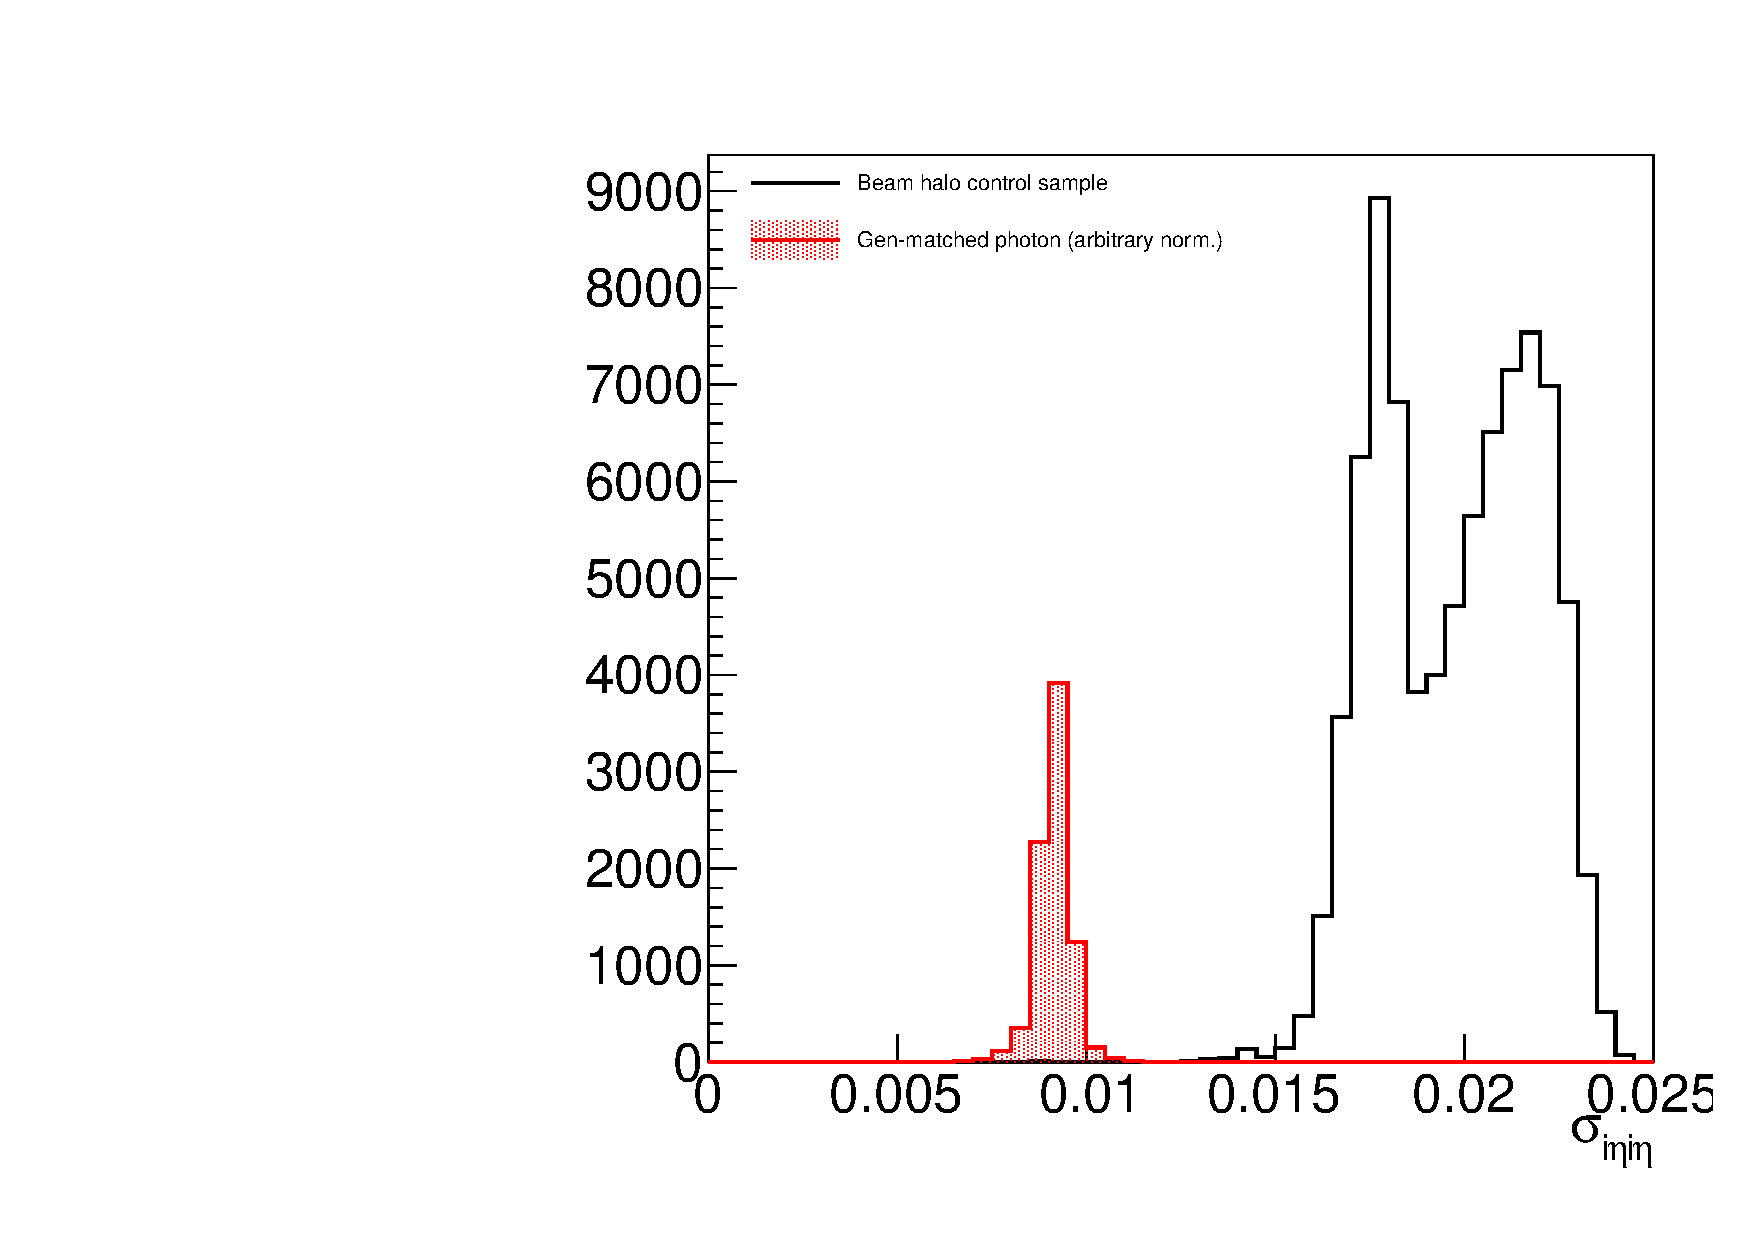
\includegraphics[width=0.45\textwidth]{Reconstruction/Figures/halo/halo_sieie.pdf}
    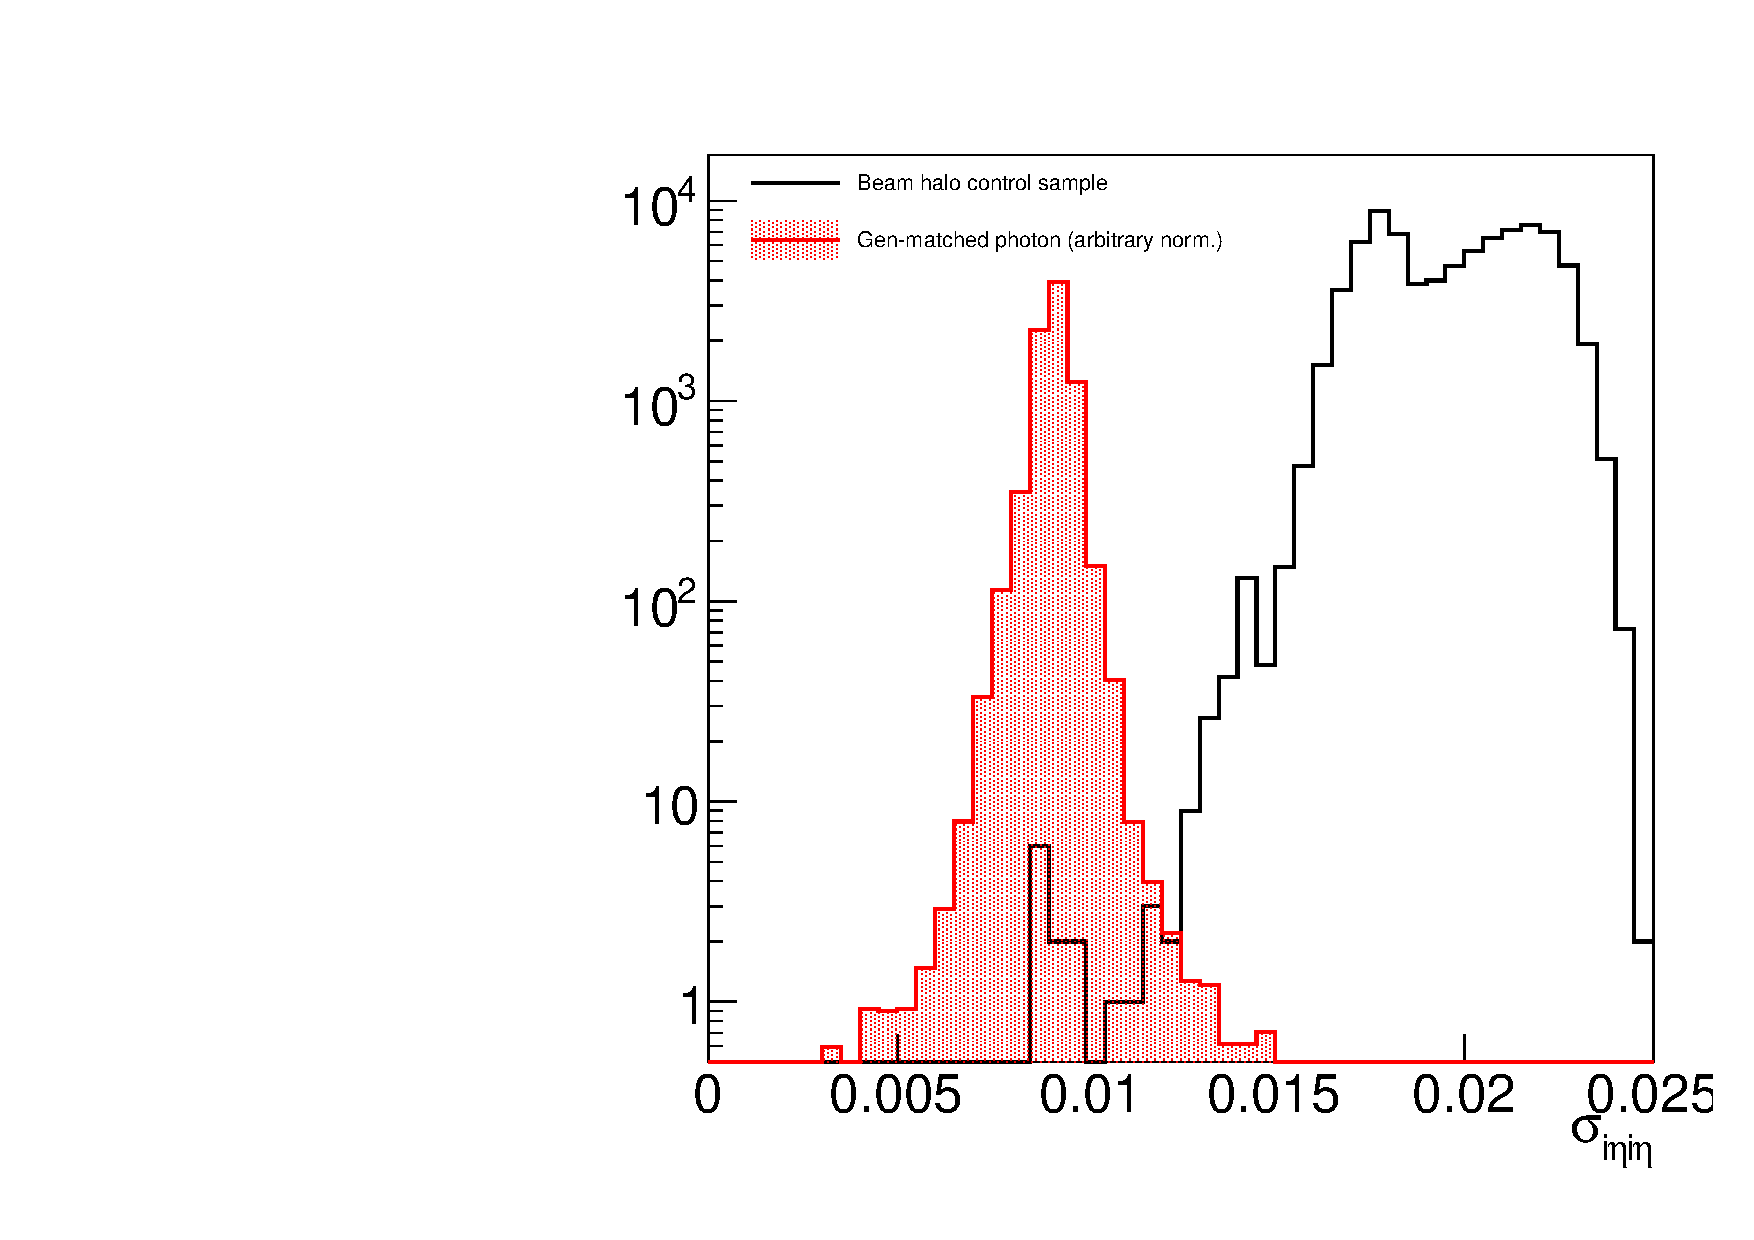
\includegraphics[width=0.45\textwidth]{Reconstruction/Figures/halo/halo_sieie_log.pdf}
    \caption{
      The \sieie distribution of the beam halo control sample and a reference distribution from truth-matched MC photons. 
      Left: linear scale, Right: log scale. 
      There is a small peak at $\sieie \sim 0.01$ in the beam halo control sample, which is not visible in linear-scale.
    }
    \label{fig:halo_sieie}
  \end{center}
\end{figure}

The contribution of real photons into the halo control sample is negligible.
This is confirmed from the \sieie\ distribution of the halo control sample and the correlation between \sieie\ and \emip\ in a MC true-photon sample.
The \sieie\ distribution of the halo control sample features a small peak at $\sieie \sim 0.01$, which can be attributed to contributions from true photons, as the photon \sieie distribution overlaid in Figure~\ref{fig:halo_sieie} suggests. 
However, the contribution of true photons diminishes rapidly with increasing \sieie. 
Additionally, Figure~\ref{fig:sieie_mip_corr} illustrates that the shape of the true-photon \sieie does not change significantly with respect to \emip. 
From these two observations, we can see that there are is only a negligible number of true photons in the halo control sample.

\begin{figure}[tbp]
  \begin{center}
    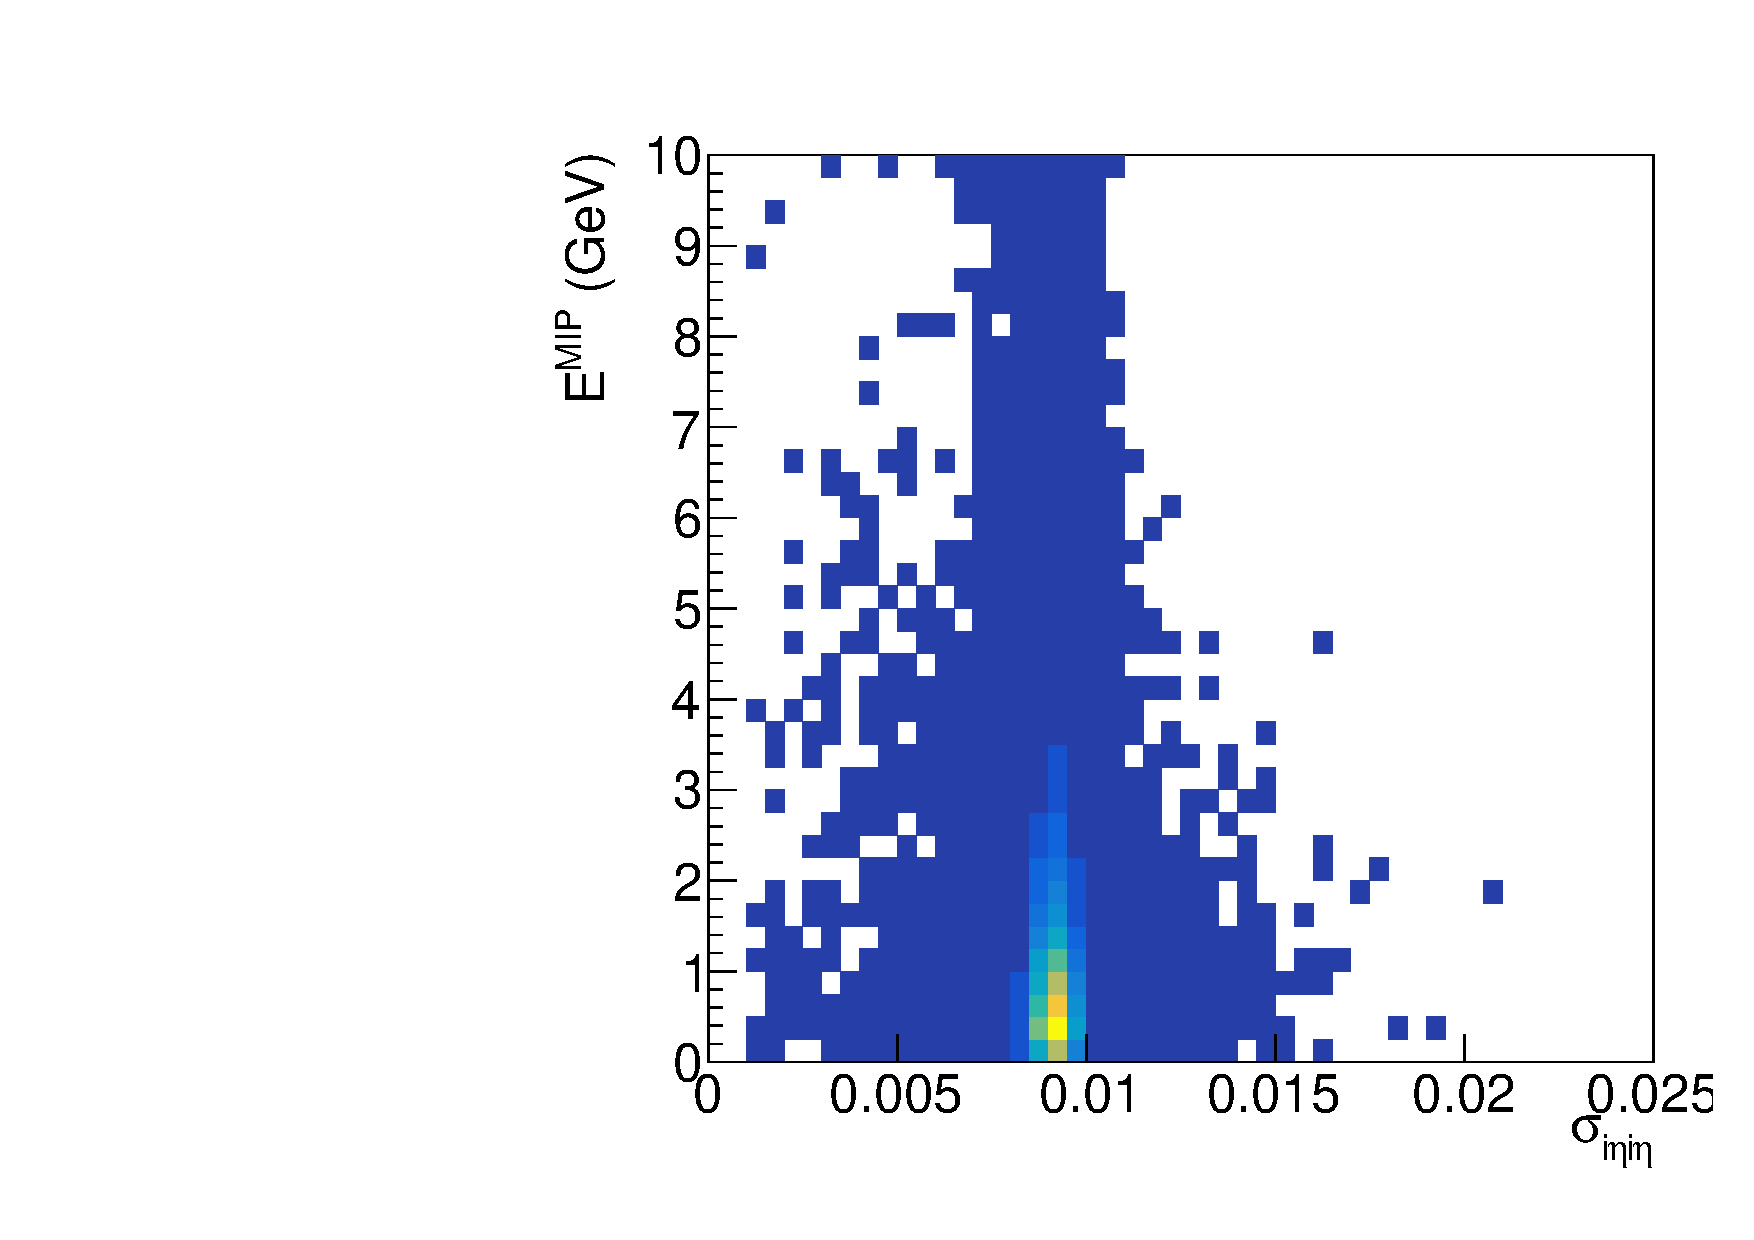
\includegraphics[width=0.45\textwidth]{Reconstruction/Figures/halo/sieie_mip_corr.pdf}
    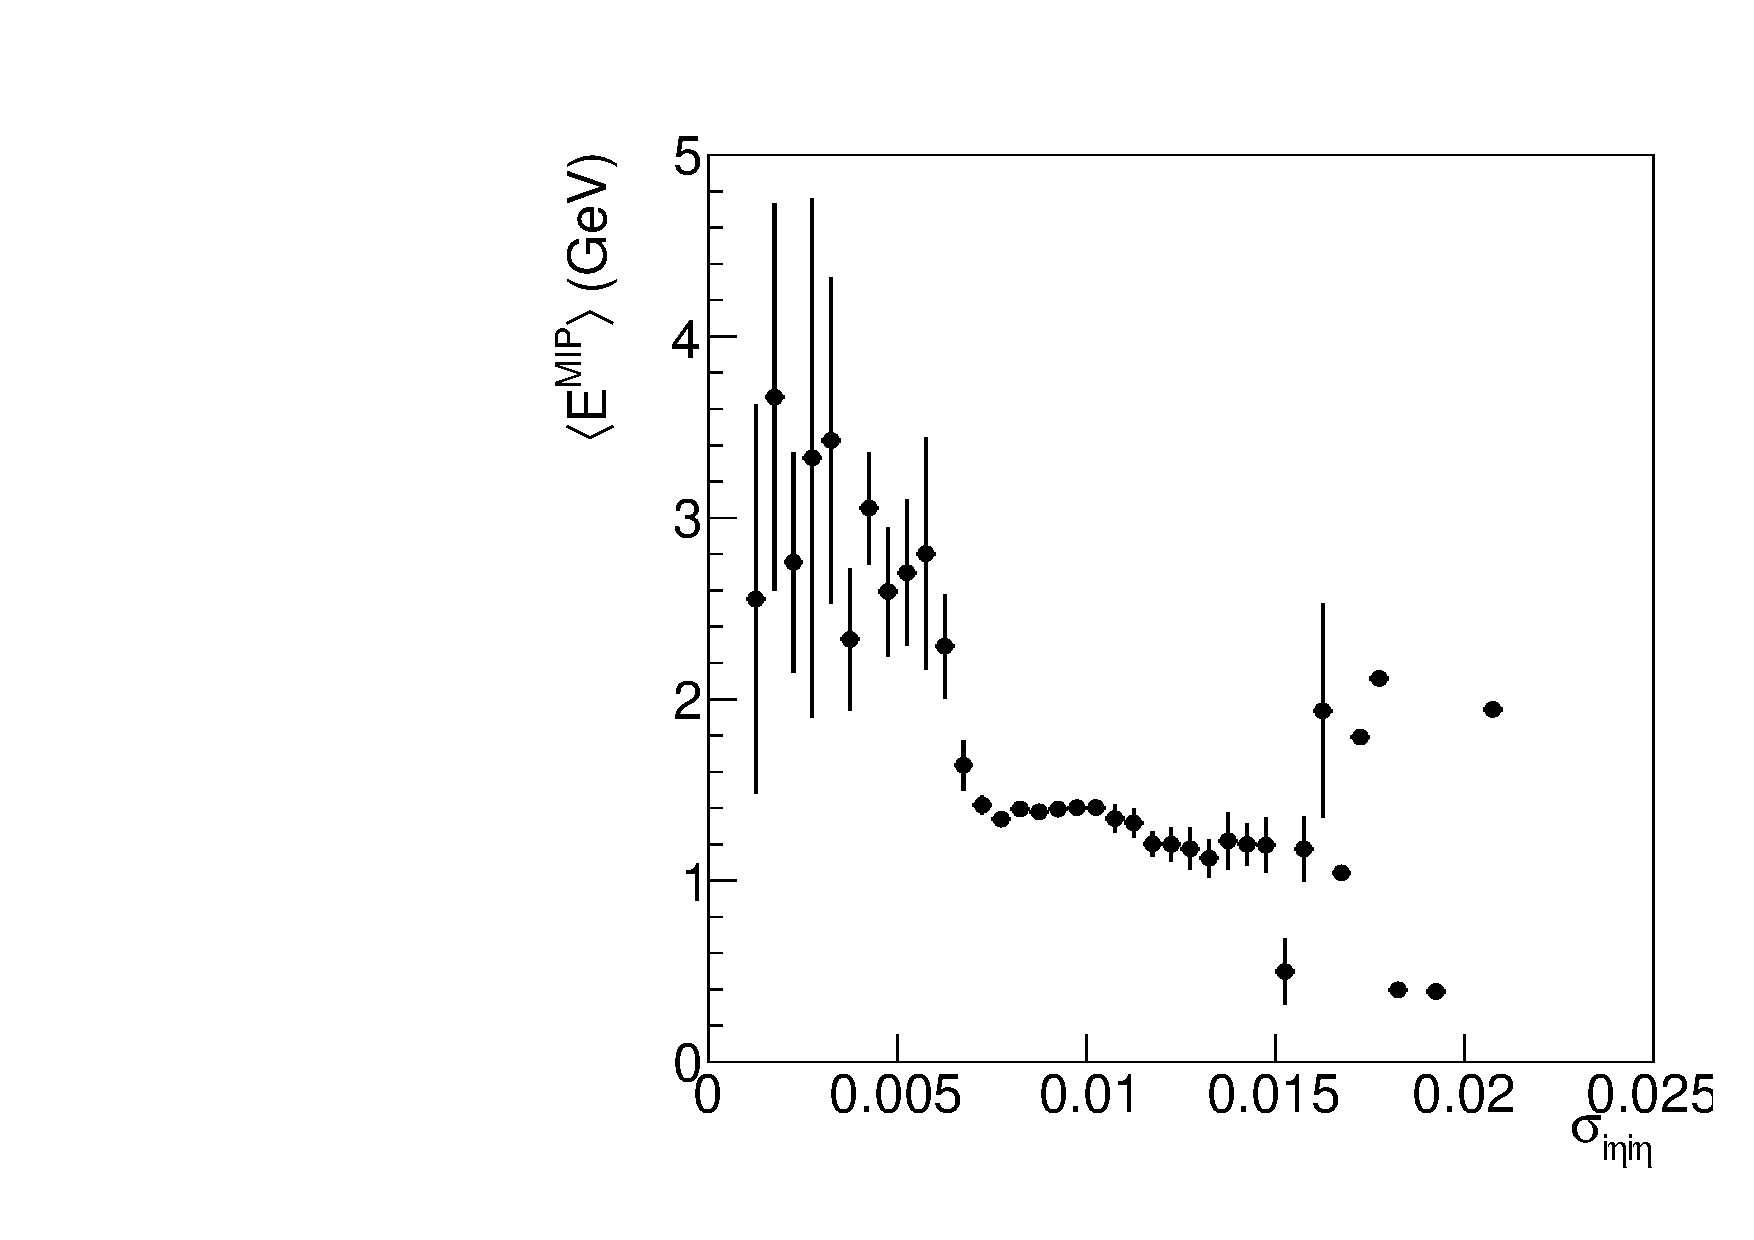
\includegraphics[width=0.45\textwidth]{Reconstruction/Figures/halo/sieie_mip_prof.pdf}
    \caption{
      Correlation between \sieie and \emip\ in truth-matched MC photons. 
      Left: \emip-\sieie distribution.
      Right: average \emip\ in bins of \sieie.
    }
    \label{fig:sieie_mip_corr}
  \end{center}
\end{figure}

While the peaking behavior is a robust feature of the halo showers, their rate is not easily predictable. 
Therefore, the contribution from beam halo processes is estimated by a direct fit to the observed data during the signal extraction process, described in Section~\ref{sec:halo_estimate}

\subsection{ECAL Barrel Spikes Phenomenology}
\label{sec:spikes}

Noise in the photodetector or the detector electronics can result in spurious photon signals. 
Most of the time, such spurious signal is filtered out by multiple layers of protection, starting from the so-called ``spike killer'' algorithm at the Level 1 trigger~\cite{CMS_AN_2010-357}. 
Nevertheless, in rare cases, noise in a single ECAL channel coincides with pileup or other energy deposit in the nearby crystals and appear as a high-energy photon cluster.

\begin{figure}[tbp]
  \begin{center}
    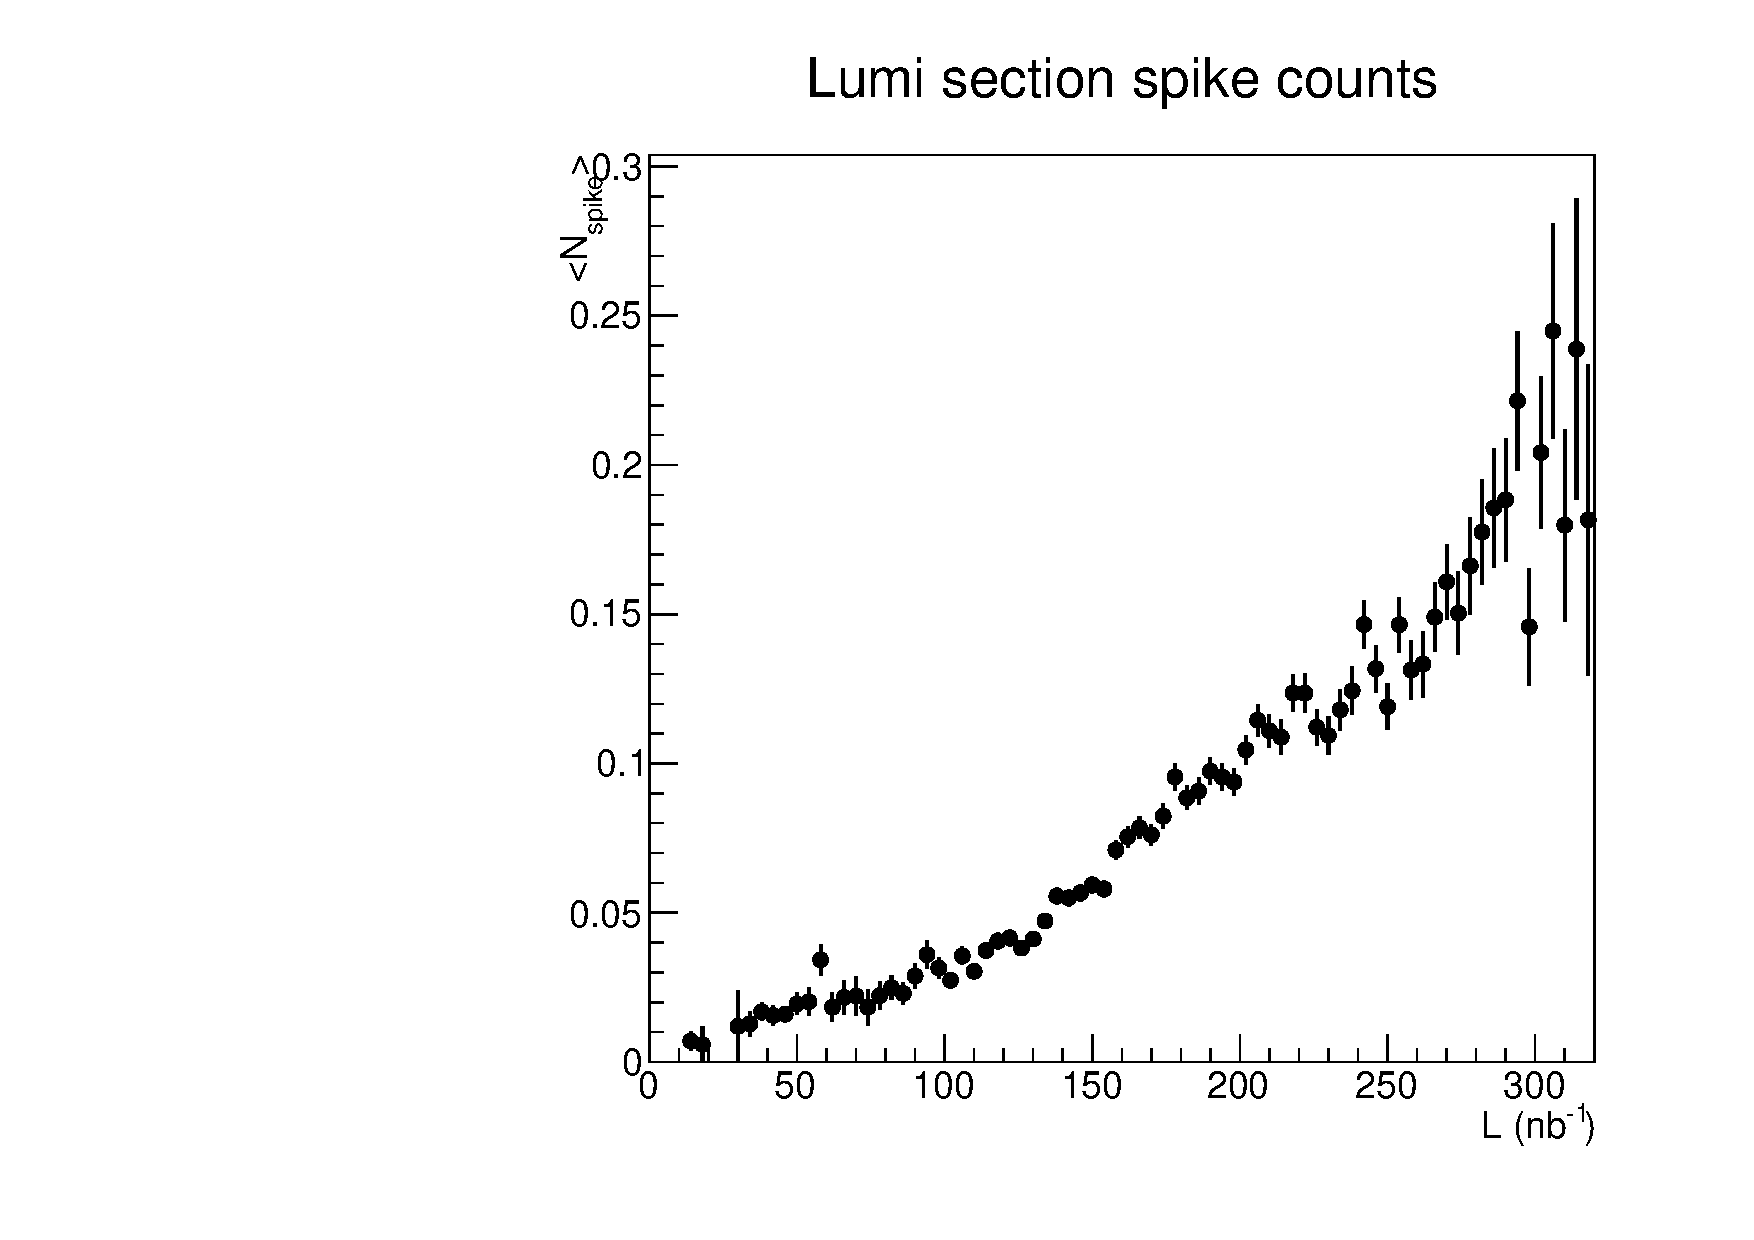
\includegraphics[width=0.45\textwidth]{Reconstruction/Figures/spikes/spike_lumi_scaling.pdf}
    \caption{
      Average number of spike clusters in a luminosity section, identified by $\sieie < 0.001$ and $E > 50\GeV$, in muon-triggered events, versus integrated luminosity of the luminosity section.
    }
    \label{fig:spike_lumi_scaling}
  \end{center}
\end{figure}

The origin of ECAL spikes is believed to be interactions of neutrons and other hadronic particles (collectively called neutral hadrons hereafter) with the photocathode material of the ECAL avalanche photo diodes (APD). 
Nuclear fission at the APD surface then causes a large electron avalanche, which is mistaken as a large photon yield scintillation in the ECAL crystal. 
Evidences supporting this hypothesis is documented in Ref.~\cite{CMS_AN_2010-357}. 
In Figure~\ref{fig:spike_lumi_scaling}, scaling of the rate of spikes with the instantaneous luminosity is confirmed, up to much higher luminosity values than was observed at the time when Ref.~\cite{CMS_AN_2010-357} was written.

A known feature of such spurious photon clusters is that the recorded pulse shape of the seed crystal, \ie, the channel with the noise, is not what is expected from a real electromagnetic shower in ECAL. 
In particular, this translates to a distinctive early rec hit time distribution, since the rec hit time is extracted from a fit to the pulse shape assuming a normal pulse.

In the normal CMS data reconstruction, rec hits that are tagged as spike-like are ignored in clustering. 
Rec hits are tagged as spikes if there is very little energy deposit recorded in the surrounding crystals, or if the reconstructed time is out of an allowed window.
Identical algorithms are employed in the HLT and offline reconstructions.

\begin{figure}[tbp]
  \begin{center}
    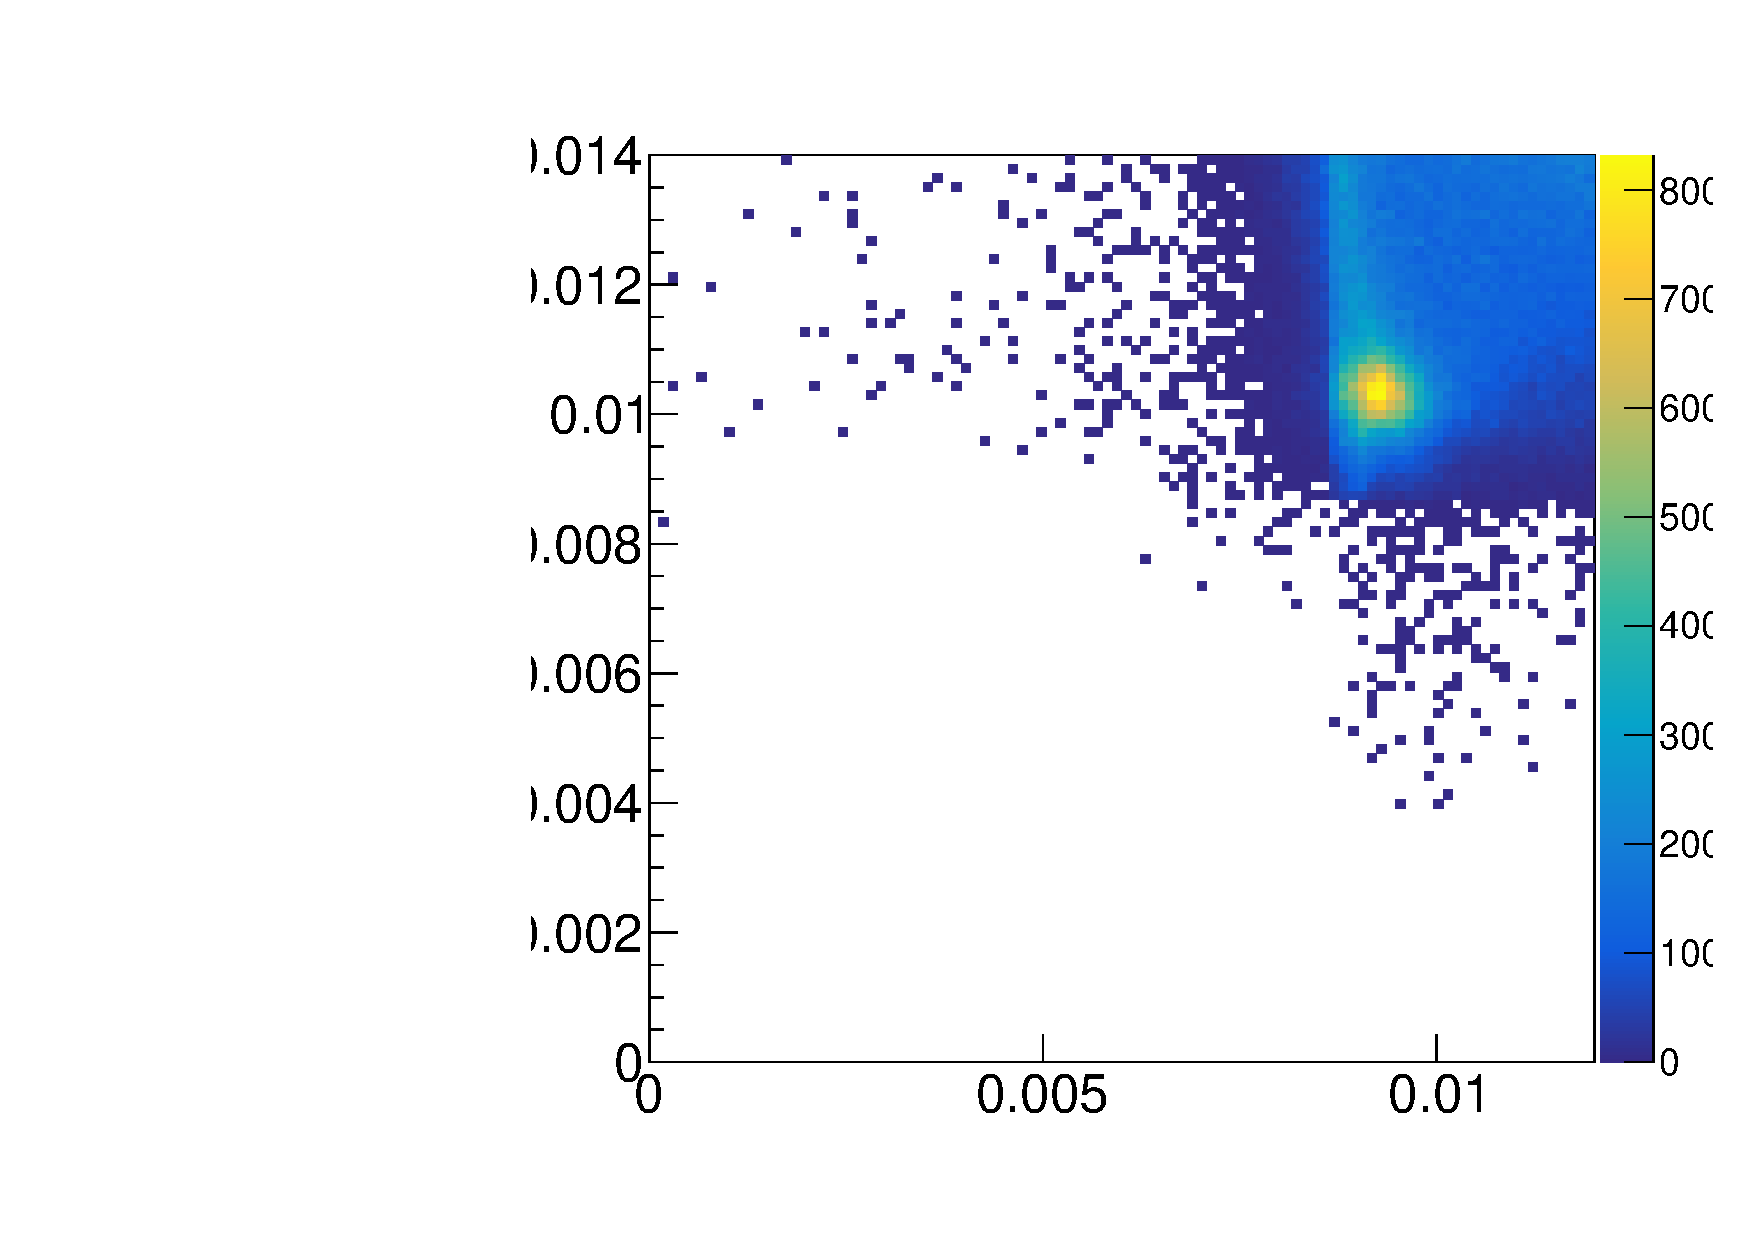
\includegraphics[width=0.45\textwidth]{Reconstruction/Figures/spikes/showershapes_standard.pdf}
    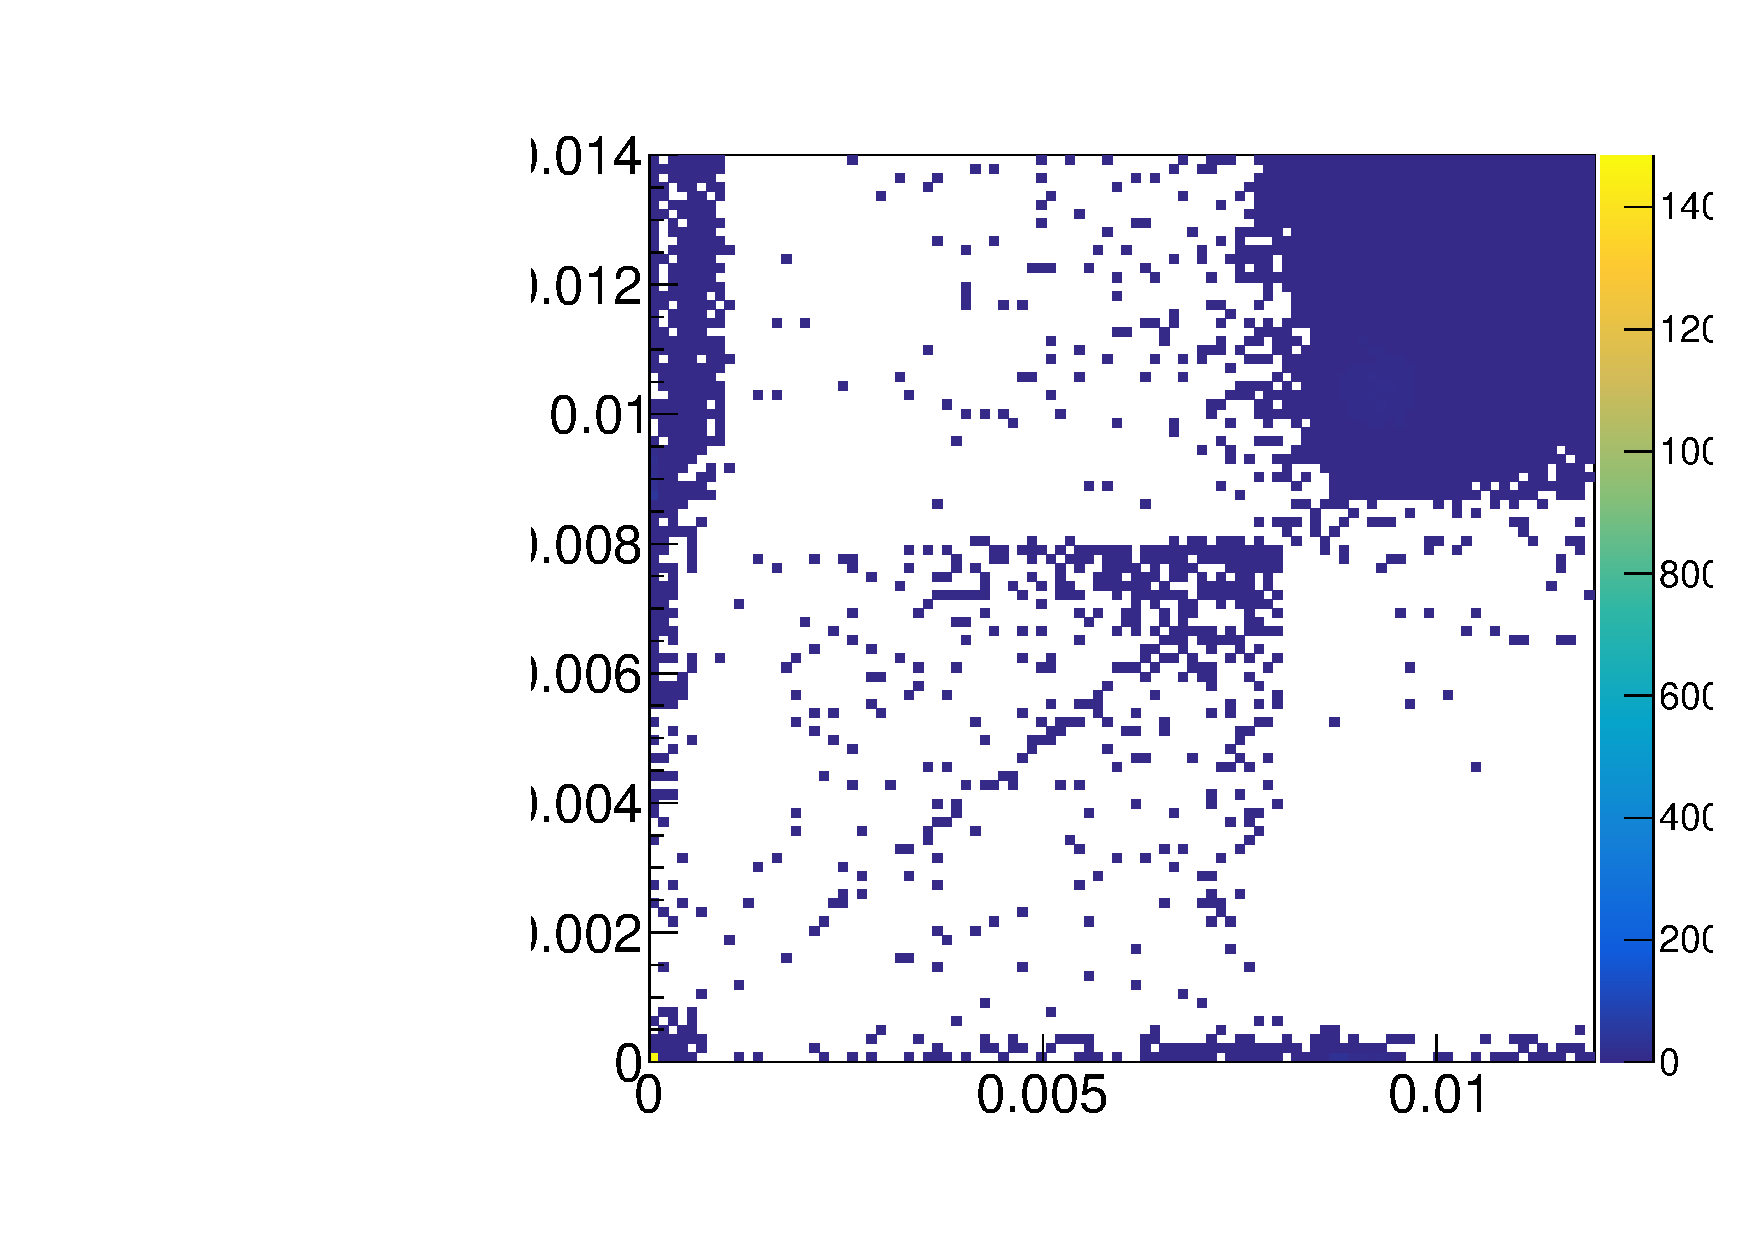
\includegraphics[width=0.45\textwidth]{Reconstruction/Figures/spikes/showershapes_uncleaned.pdf}
    \caption{
      Two-dimensional distributions in \sipip\ and \sieie\ of ECAL clusters in the standard reconstruction (left) and the special reconstruction with no spike cleaning (right).
    }
    \label{fig:showershape_map}
  \end{center}
\end{figure}

To study an unbiased spike sample, ECAL DIGI samples stored in the SingleMuon AOD datasets are reconstructed into ECAL clusters with no spike cleaning applied. 
DIGIs associated with the standard and ``uncleaned'' photon objects are stored in AOD, and ones for the uncleaned photons is rich in spike-like hits. 
Figure~\ref{fig:showershape_map} shows how narrow clusters are cleaned away in the normal reconstruction.

\begin{figure}[tbp]
  \begin{center}
    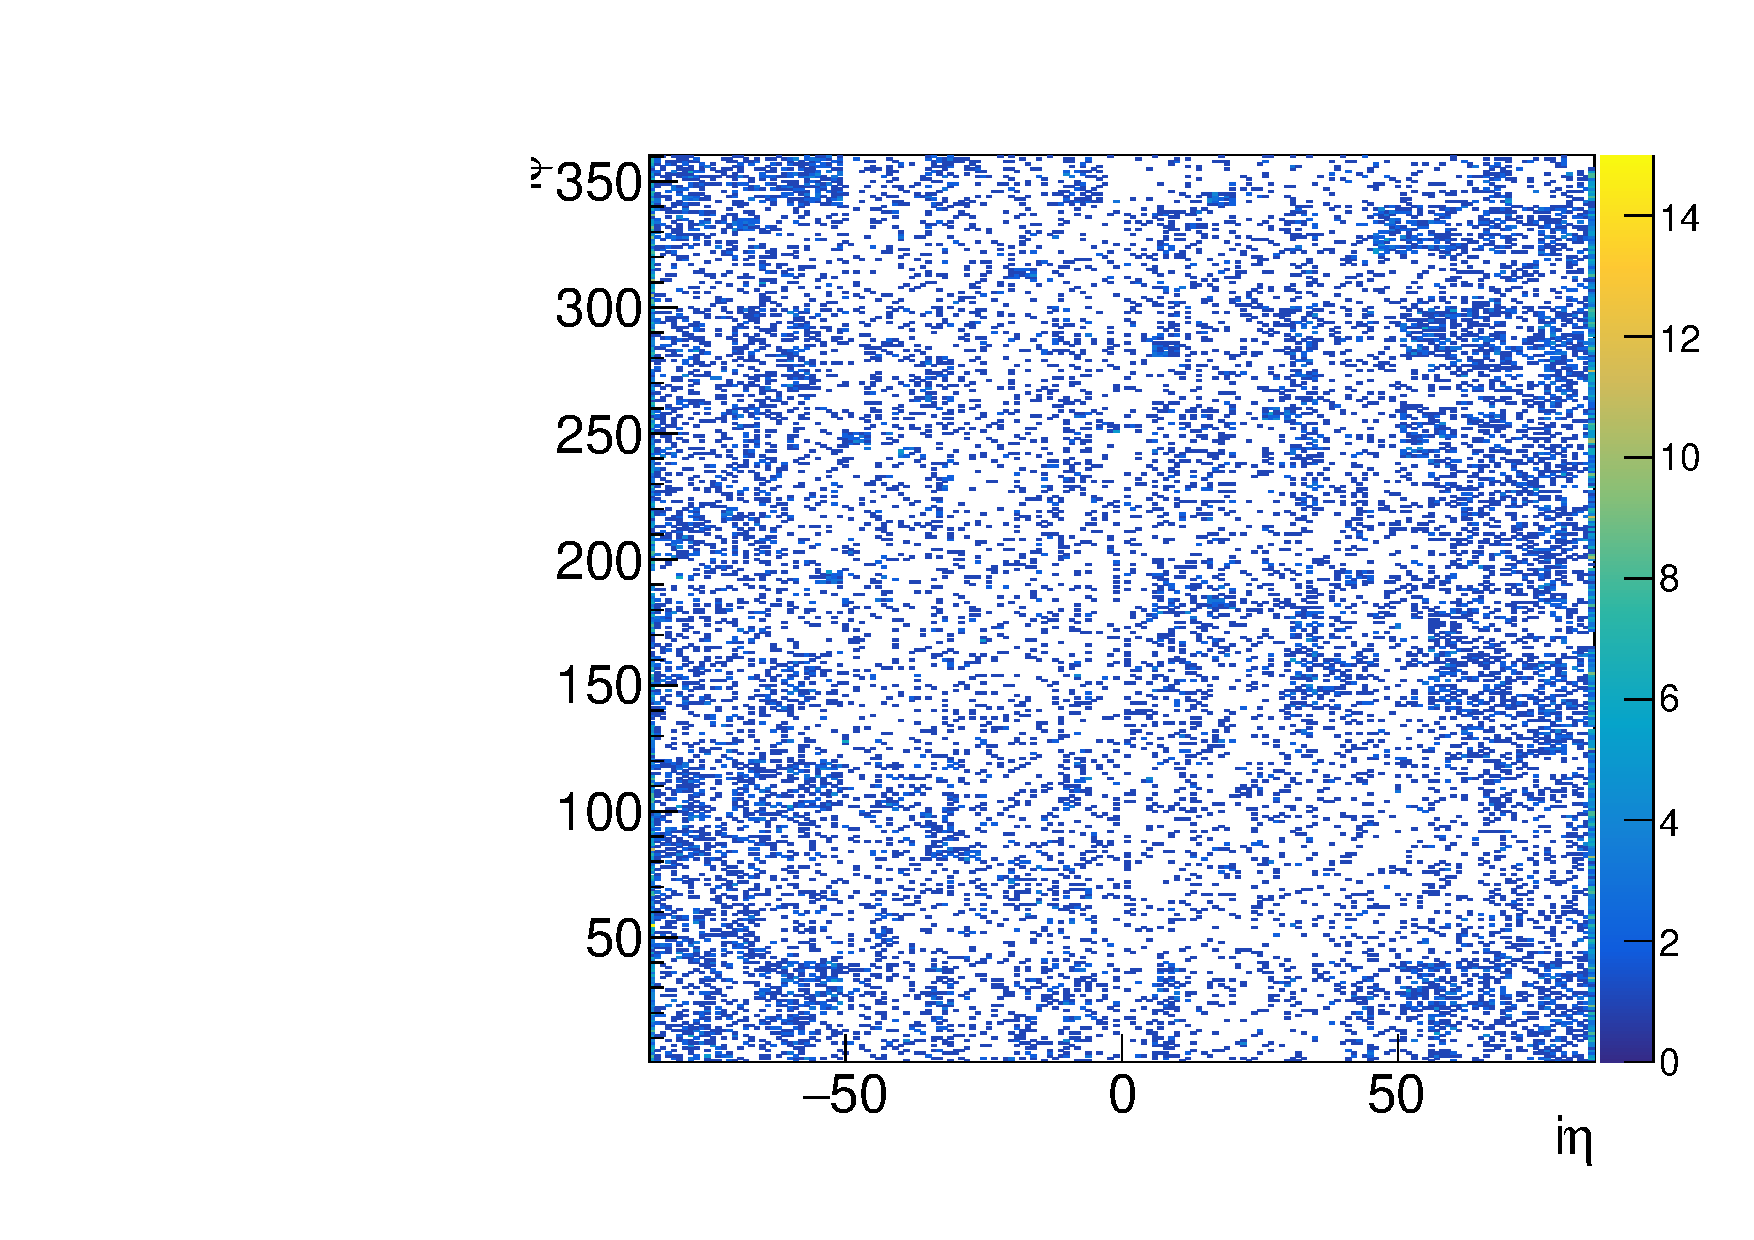
\includegraphics[width=0.45\textwidth]{Reconstruction/Figures/spikes/spike_map.pdf}
    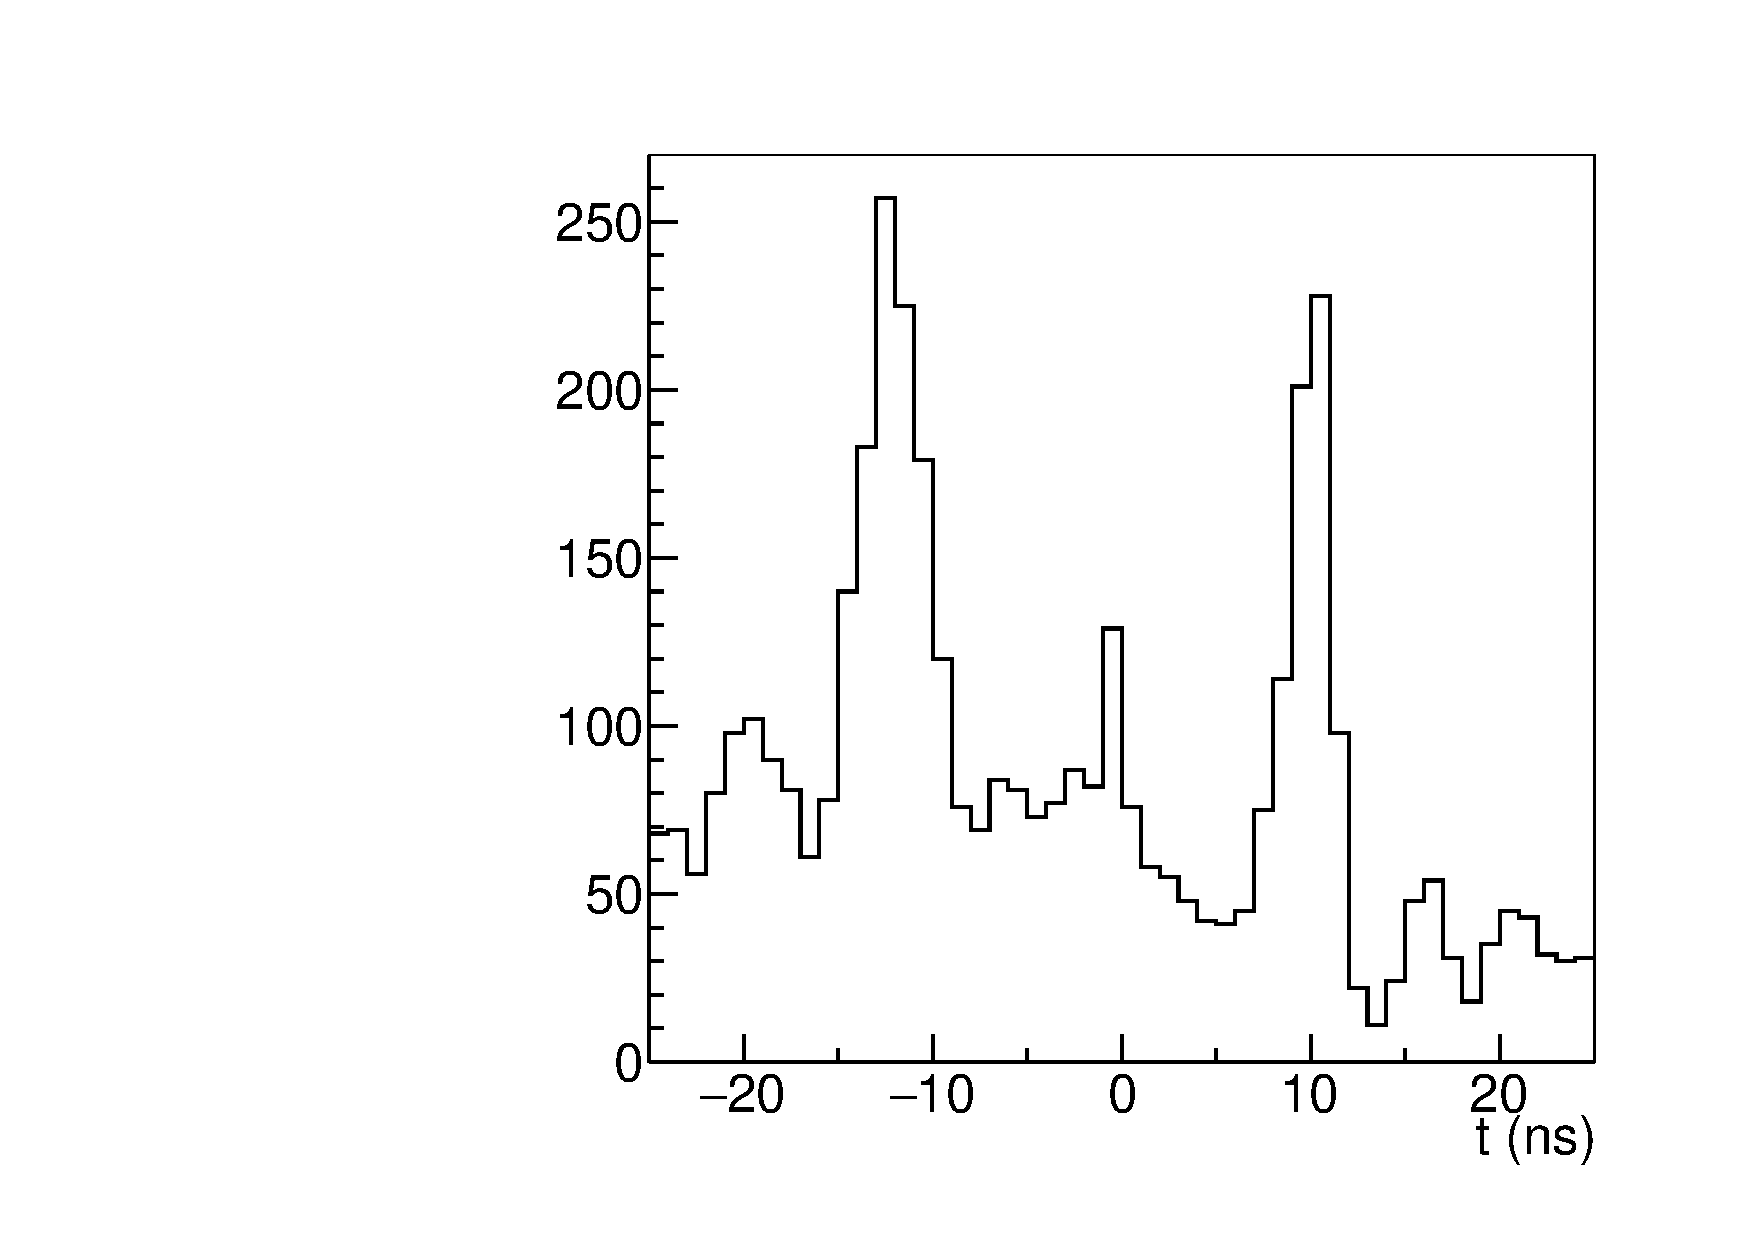
\includegraphics[width=0.45\textwidth]{Reconstruction/Figures/spikes/spike_time.pdf}
    \caption{
      $\eta$--$\phi$ and time distributions of seed hits of narrow ($\sieie < 0.001$) clusters.
    }
    \label{fig:spike_distributions}
  \end{center}
\end{figure}

Figure~\ref{fig:spike_distributions} shows the spacial and temporal distributions of the rec hits seeding narrow ($\sieie < 0.001$) clusters. 
The spacial distribution appears mostly random, indicating that there is no single source of spike-like rec hits. 
The two highest peaks in the time distribution at $t \sim -15\ns$ and $t \sim 10\ns$ are characteristic of pulse shapes, which rise faster than the pulse from the normal scintillation. 
The second peak is understood to come from the next bunch crossing.

\begin{figure}[tbp]
  \begin{center}
    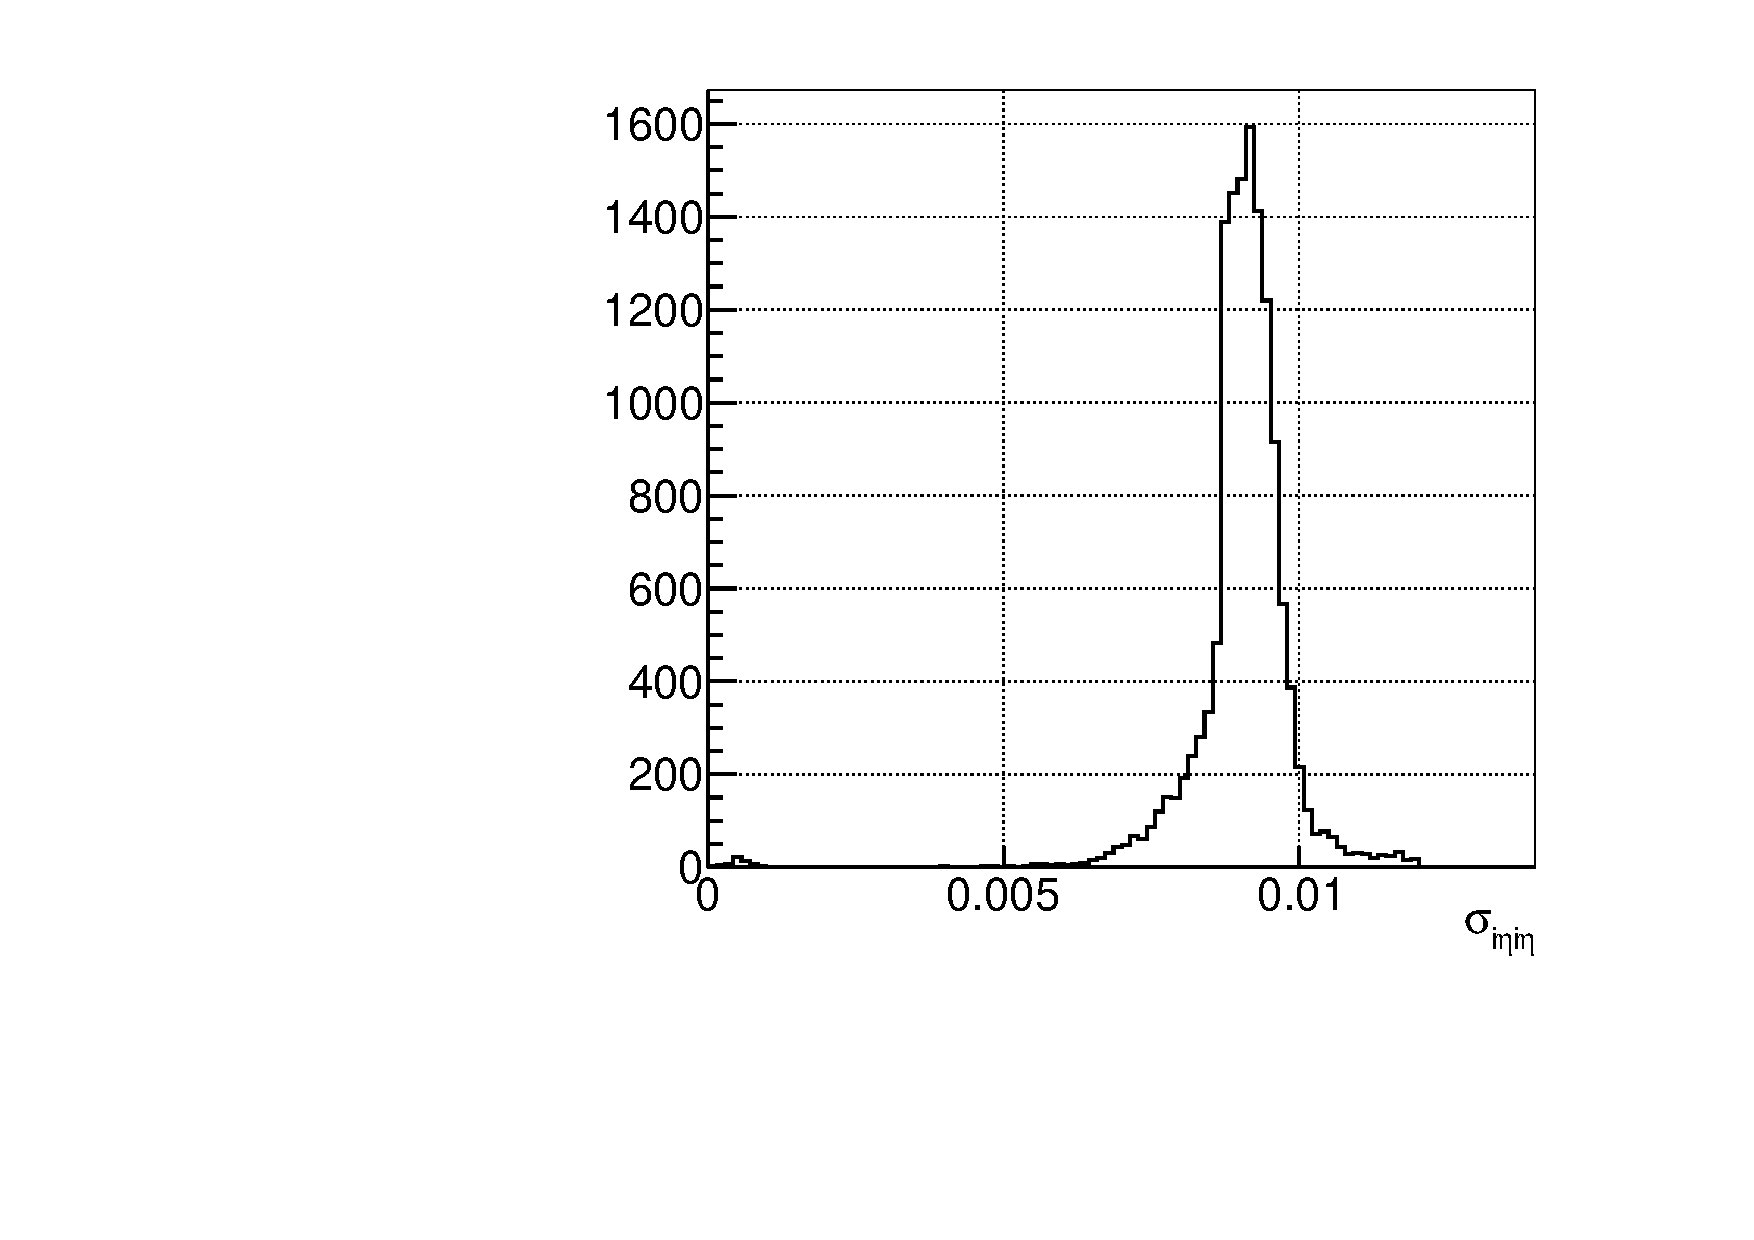
\includegraphics[width=0.45\textwidth]{Reconstruction/Figures/spikes/sieie_mc.pdf}
    \caption{
      \sieie distribution of uncleaned clusters from \gj\ MC simulation.
    }
    \label{fig:sieie_mc}
  \end{center}
\end{figure}

The small peak at $t\sim 0$ in the time distribution of Fig.~\ref{fig:spike_distributions} is due to actual ``physical'' clusters that happened to have a very narrow cluster shape. 
By processing the \gj\ MC simulation events through this special reconstruction, we see that about 0.5\% of ECAL clusters from prompt photons have $\sieie < 0.001$ as shown in Figure~\ref{fig:sieie_mc}.

\begin{figure}[tbp]
  \begin{center}
    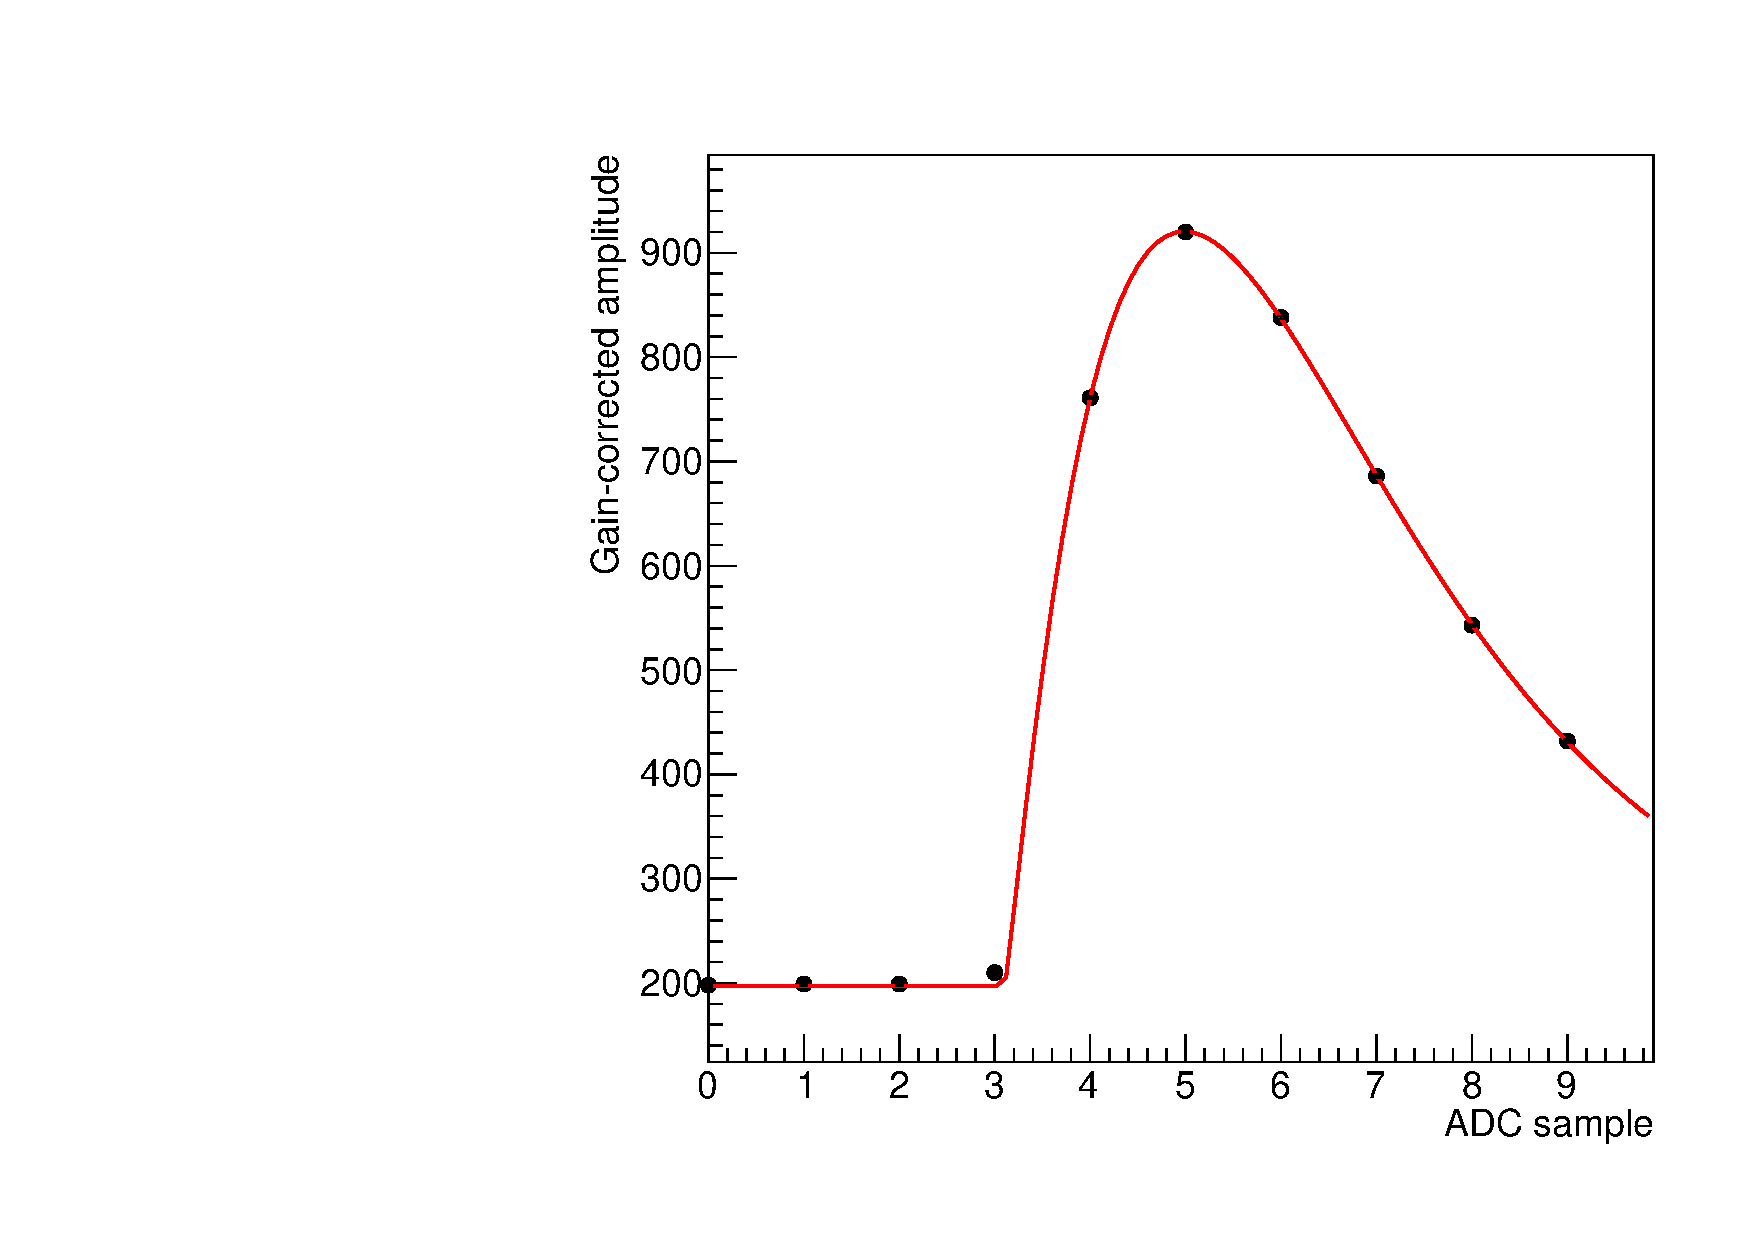
\includegraphics[width=0.3\textwidth]{Reconstruction/Figures/spikes/pulse_example_normal.pdf}
    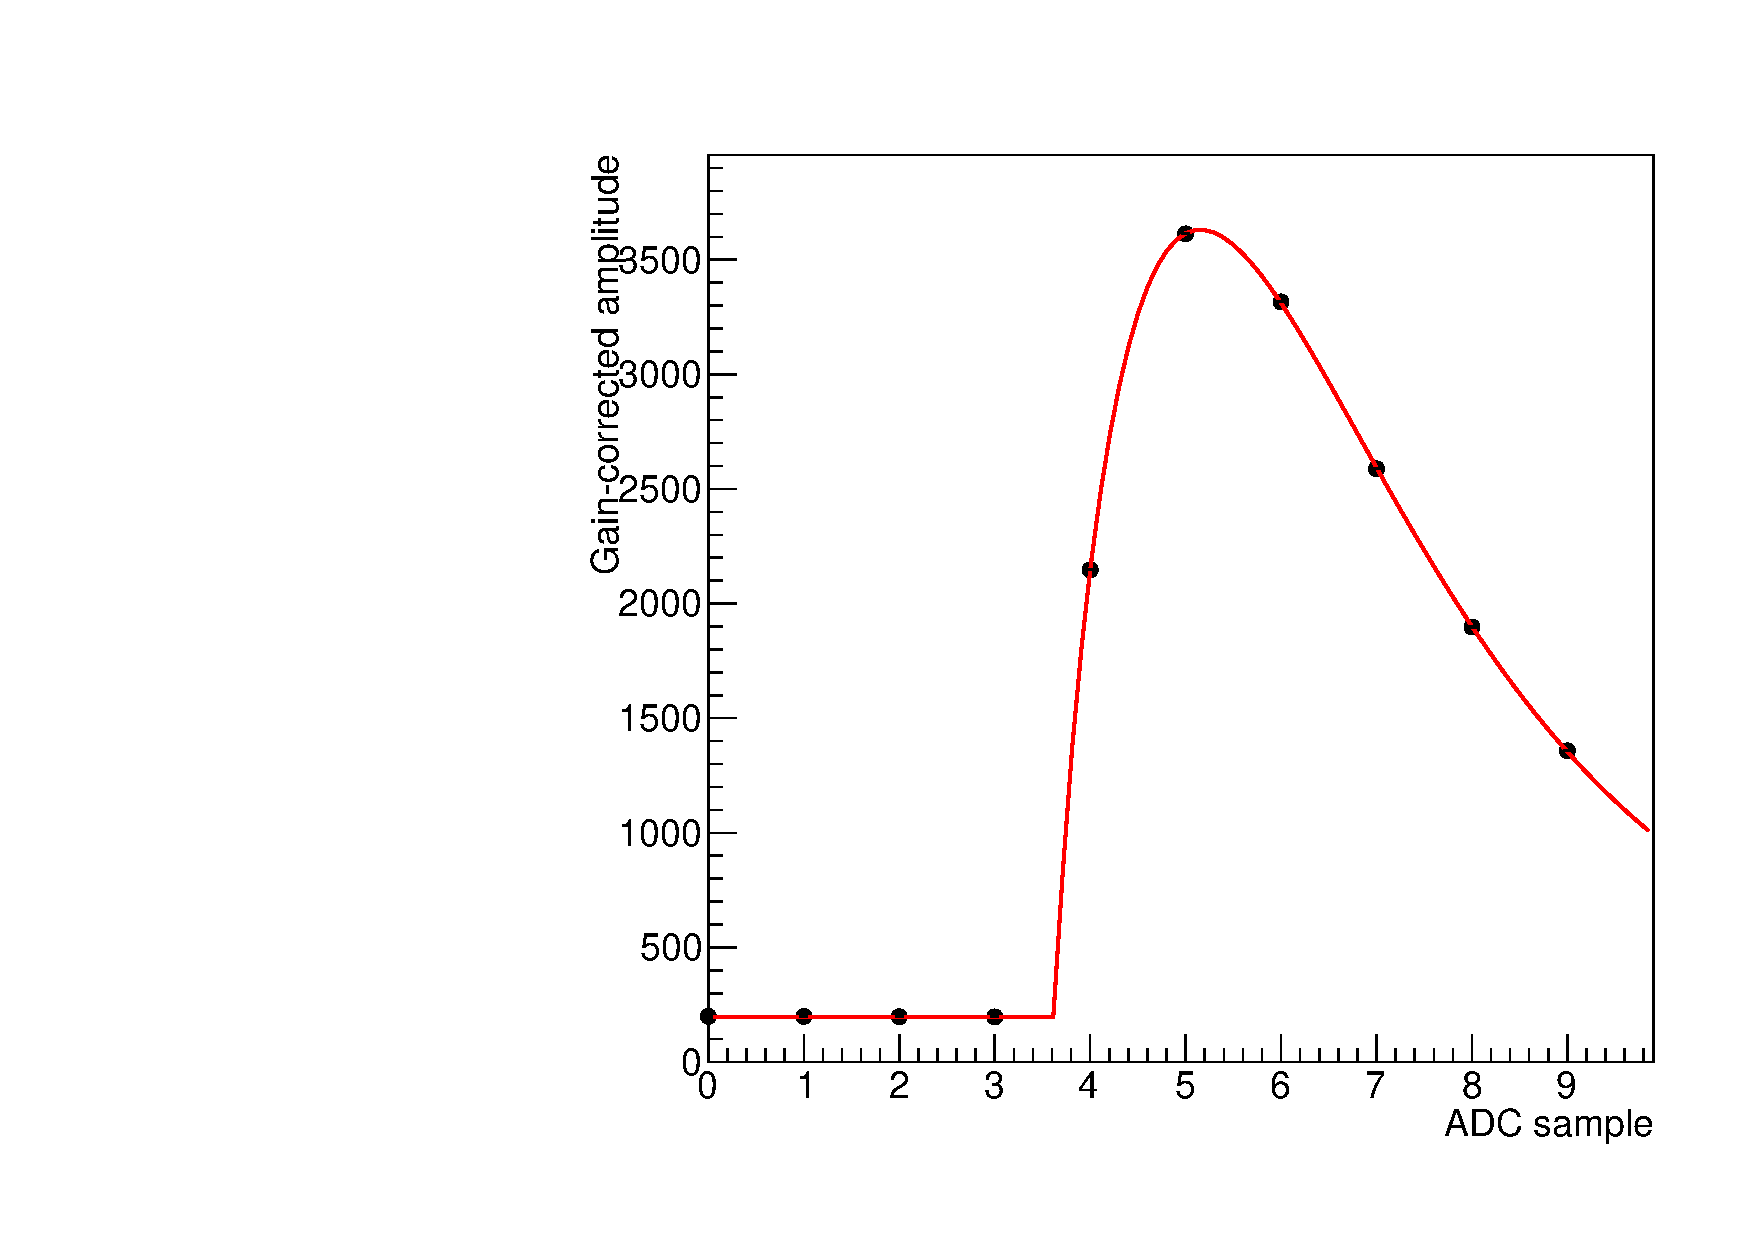
\includegraphics[width=0.3\textwidth]{Reconstruction/Figures/spikes/pulse_example_spike.pdf}
    \caption{
      Example ECAL DIGIs and corresponding pulse shapes reconstructed through $\chi^{2}$ fits of Equation~\ref{eqn:pulse_shape}, for normal (left) and spike-like (right) hits.
    }
    \label{fig:pulse_examples}
  \end{center}
\end{figure}

To understand the time distribution, one can investigate the original DIGI samples from which rec hits are made. 
At each event readout, a single ECAL channel outputs 10 ADC signals corresponding to a sampling of the analog pulse output of multi-gain preamplifier (MGPA) in range $t_{0} - 125\ns < t < t_{0} + 100\ns$, where $t_{0}$ is the time of the triggering bunch crossing. 
These 10 signal points can be described well by the formula

\begin{equation} \label{eqn:pulse_shape}
  f(t) = A \left(1 - \frac{t - \tau}{\alpha\beta}\right)^{\alpha} \exp \left(-\frac{t-\tau}{\beta}\right).
\end{equation}

\begin{figure}[tbp]
  \begin{center}
    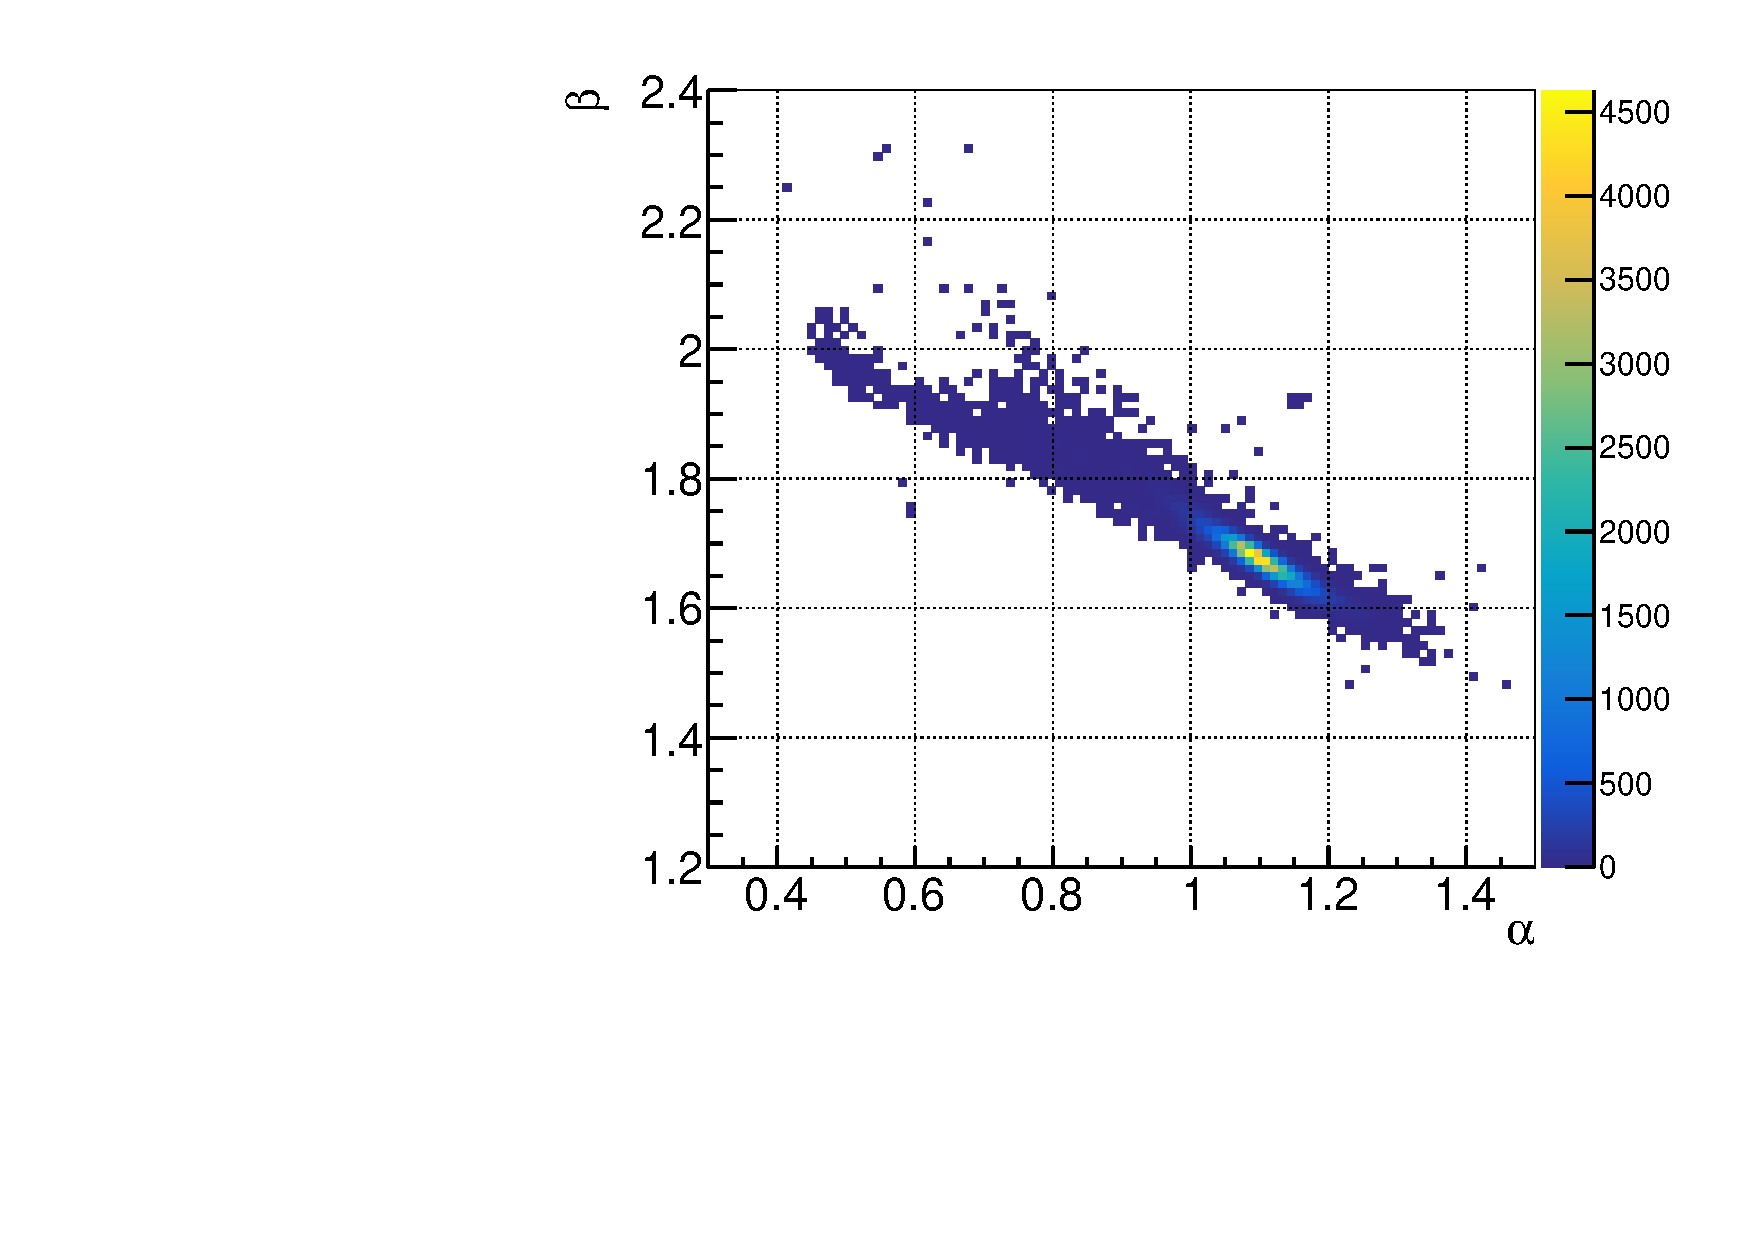
\includegraphics[width=0.45\textwidth]{Reconstruction/Figures/spikes/alphabeta_physical.pdf}
    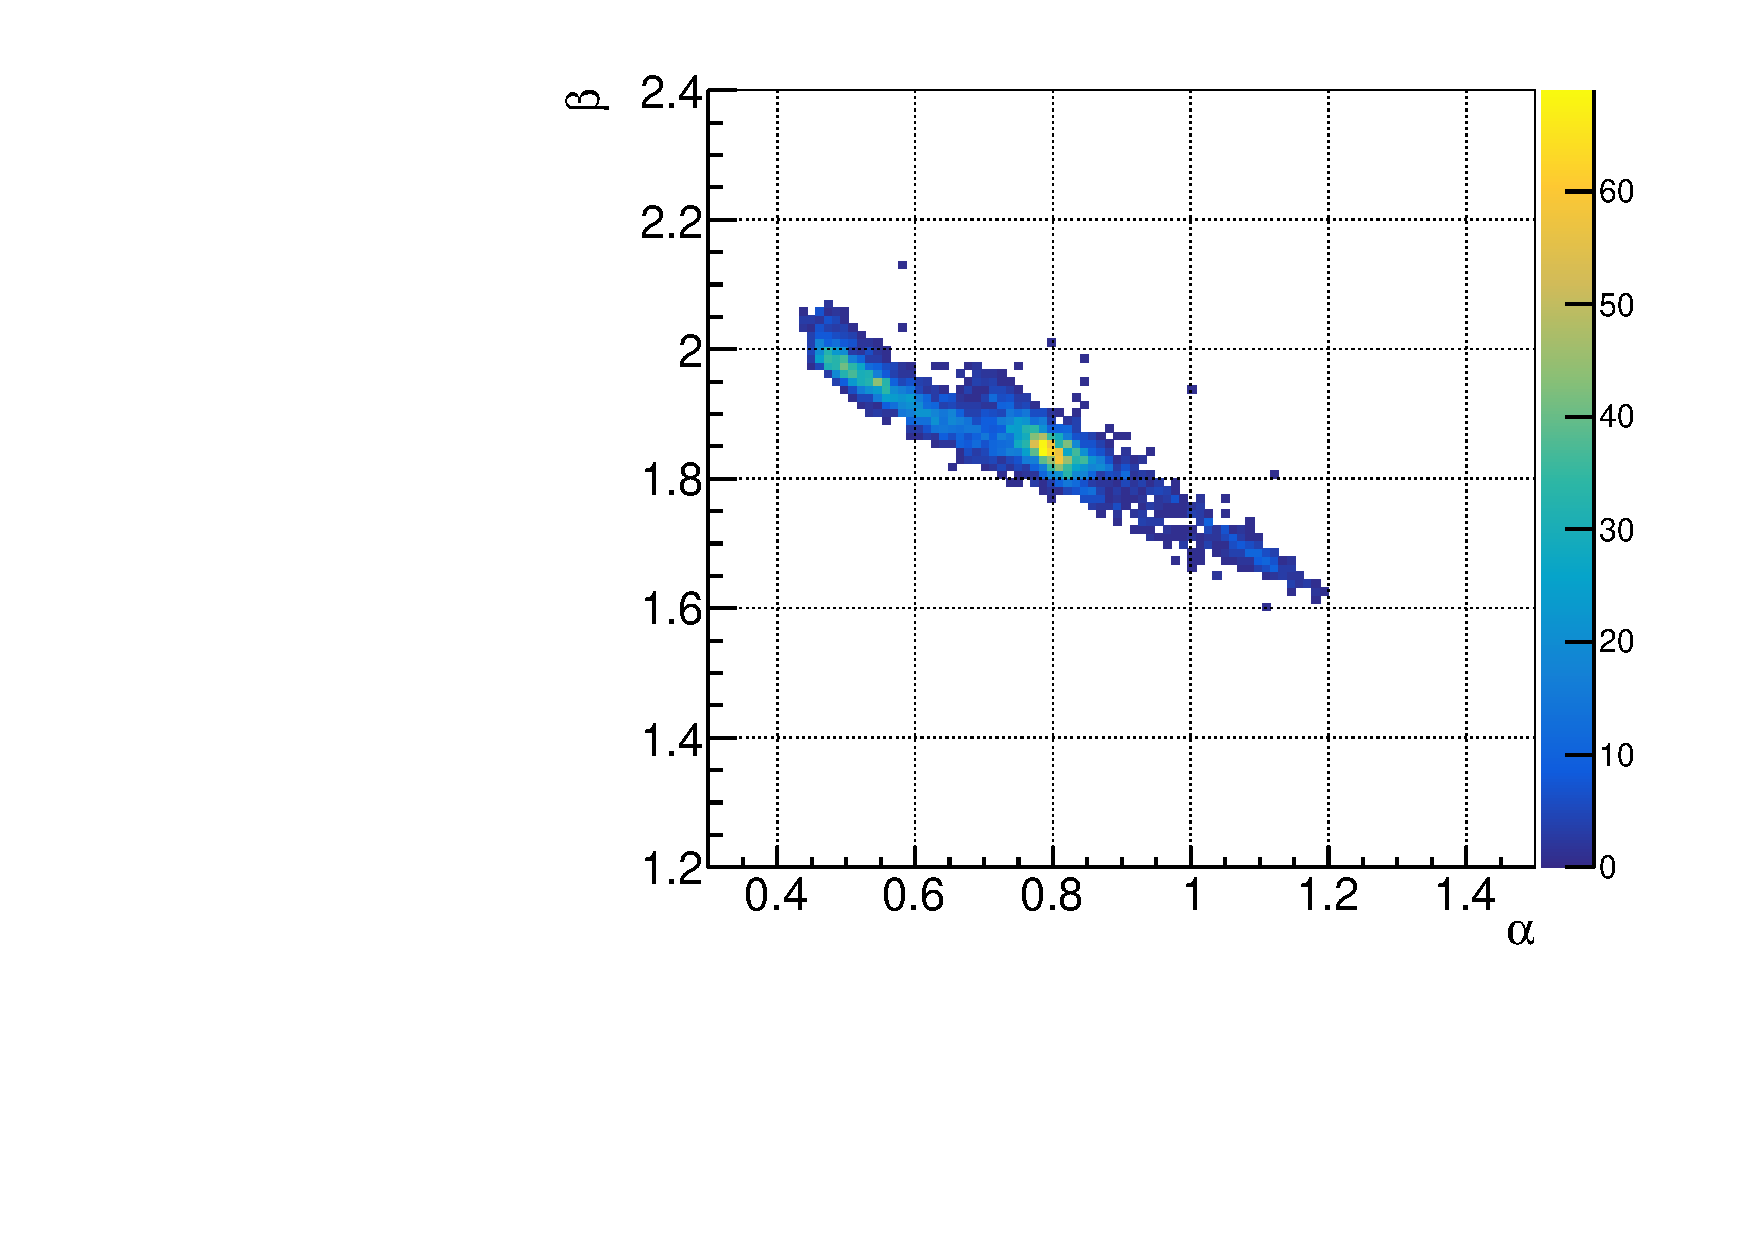
\includegraphics[width=0.45\textwidth]{Reconstruction/Figures/spikes/alphabeta_spike.pdf}
    \caption{
      $\alpha$--$\beta$ distributions of the seed hits of physical wide clusters (left) and spike-like clusters (right).
    }
    \label{fig:spike_alphabeta}
  \end{center}
\end{figure}

In the formula, parameters $A$ and $\tau$ correspond to the pulse amplitude and peak time, whereas $\alpha$ and $\beta$ control the shape of the pulse. 
Figure~\ref{fig:pulse_examples} illustrates various observed pulse shapes fit with the above formula with all parameters floating. 
A $\chi^{2}$ fit is employed using the average noise amplitude of each MGPA channel as the errors on the data points. 
The noise is measured in ECAL calibration cycles in the inter-fill period and is recorded in the conditions database.

\begin{figure}[tbp]
  \begin{center}
    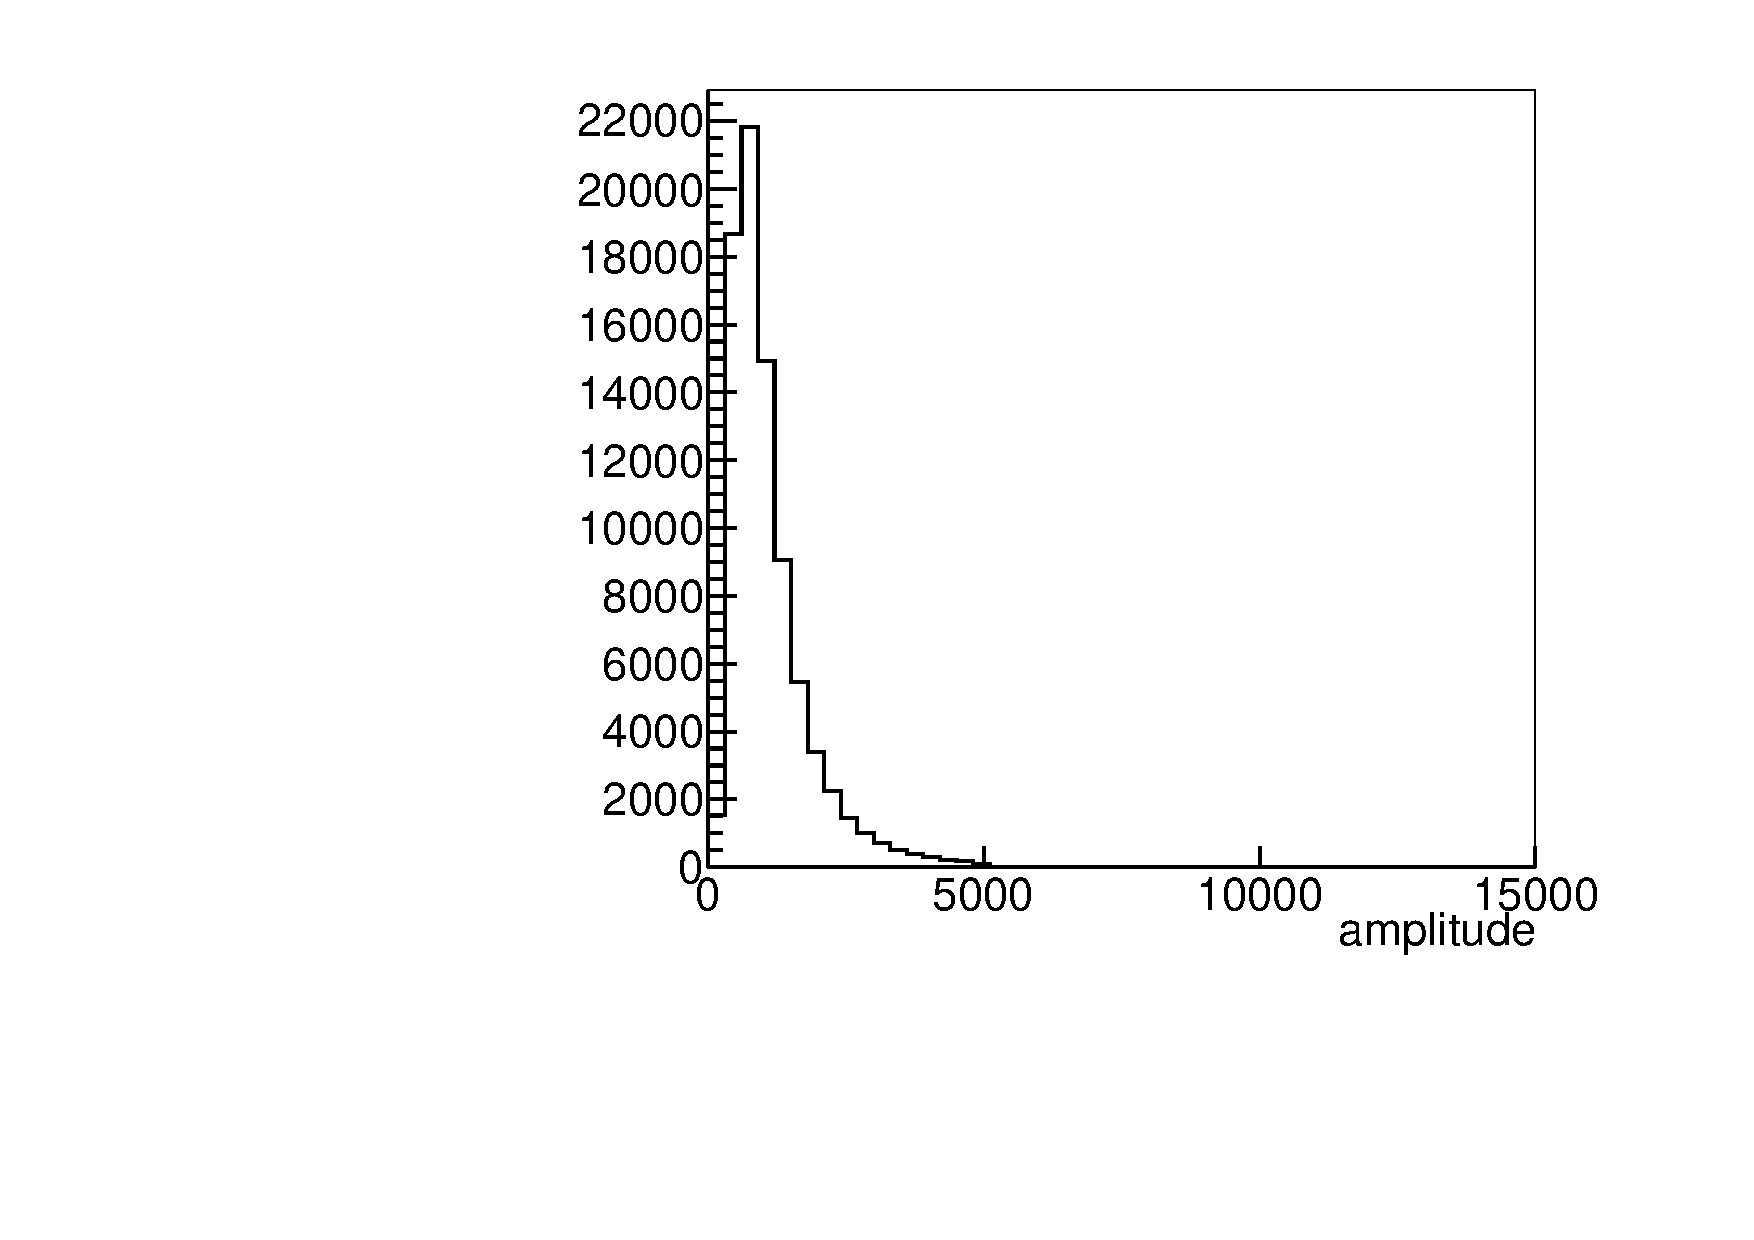
\includegraphics[width=0.3\textwidth]{Reconstruction/Figures/spikes/physical_amplitude.pdf}
    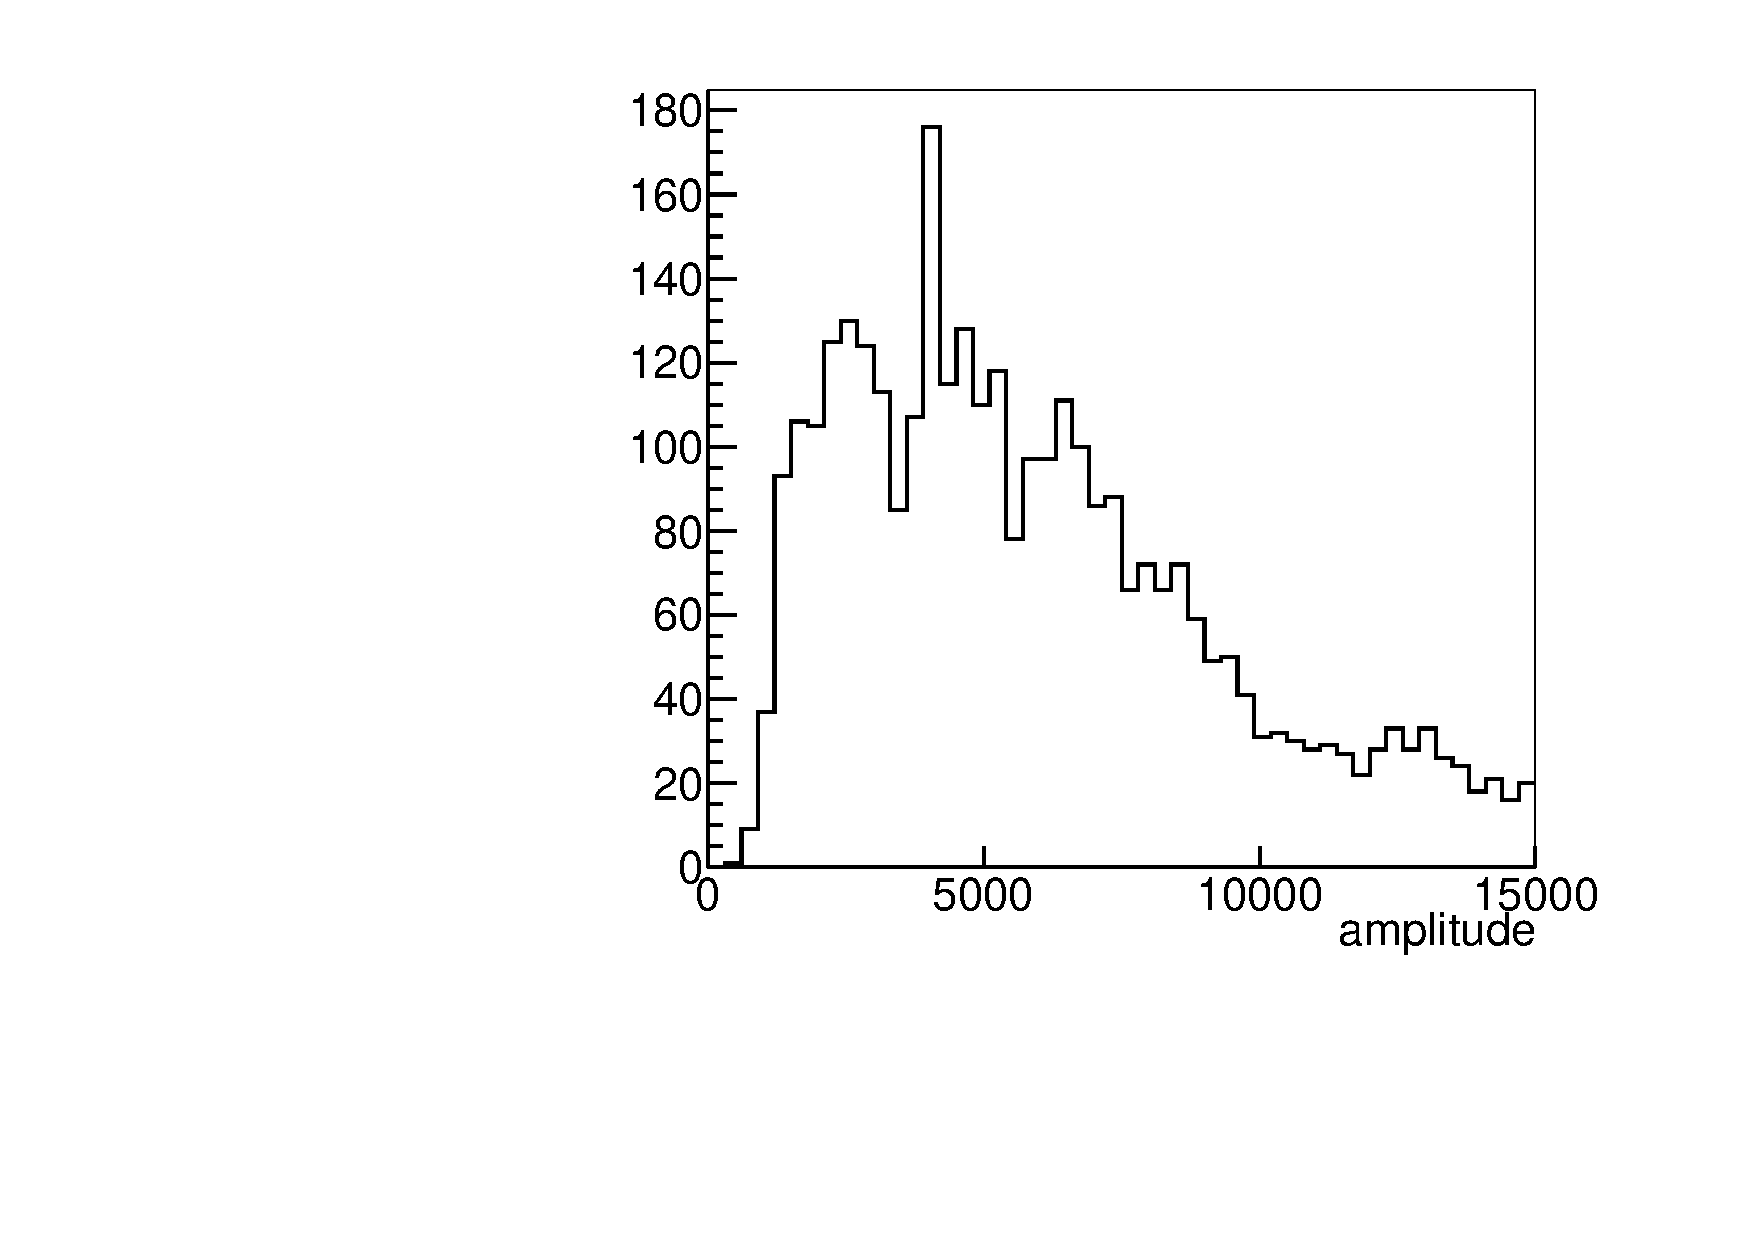
\includegraphics[width=0.3\textwidth]{Reconstruction/Figures/spikes/spike_amplitude.pdf}
    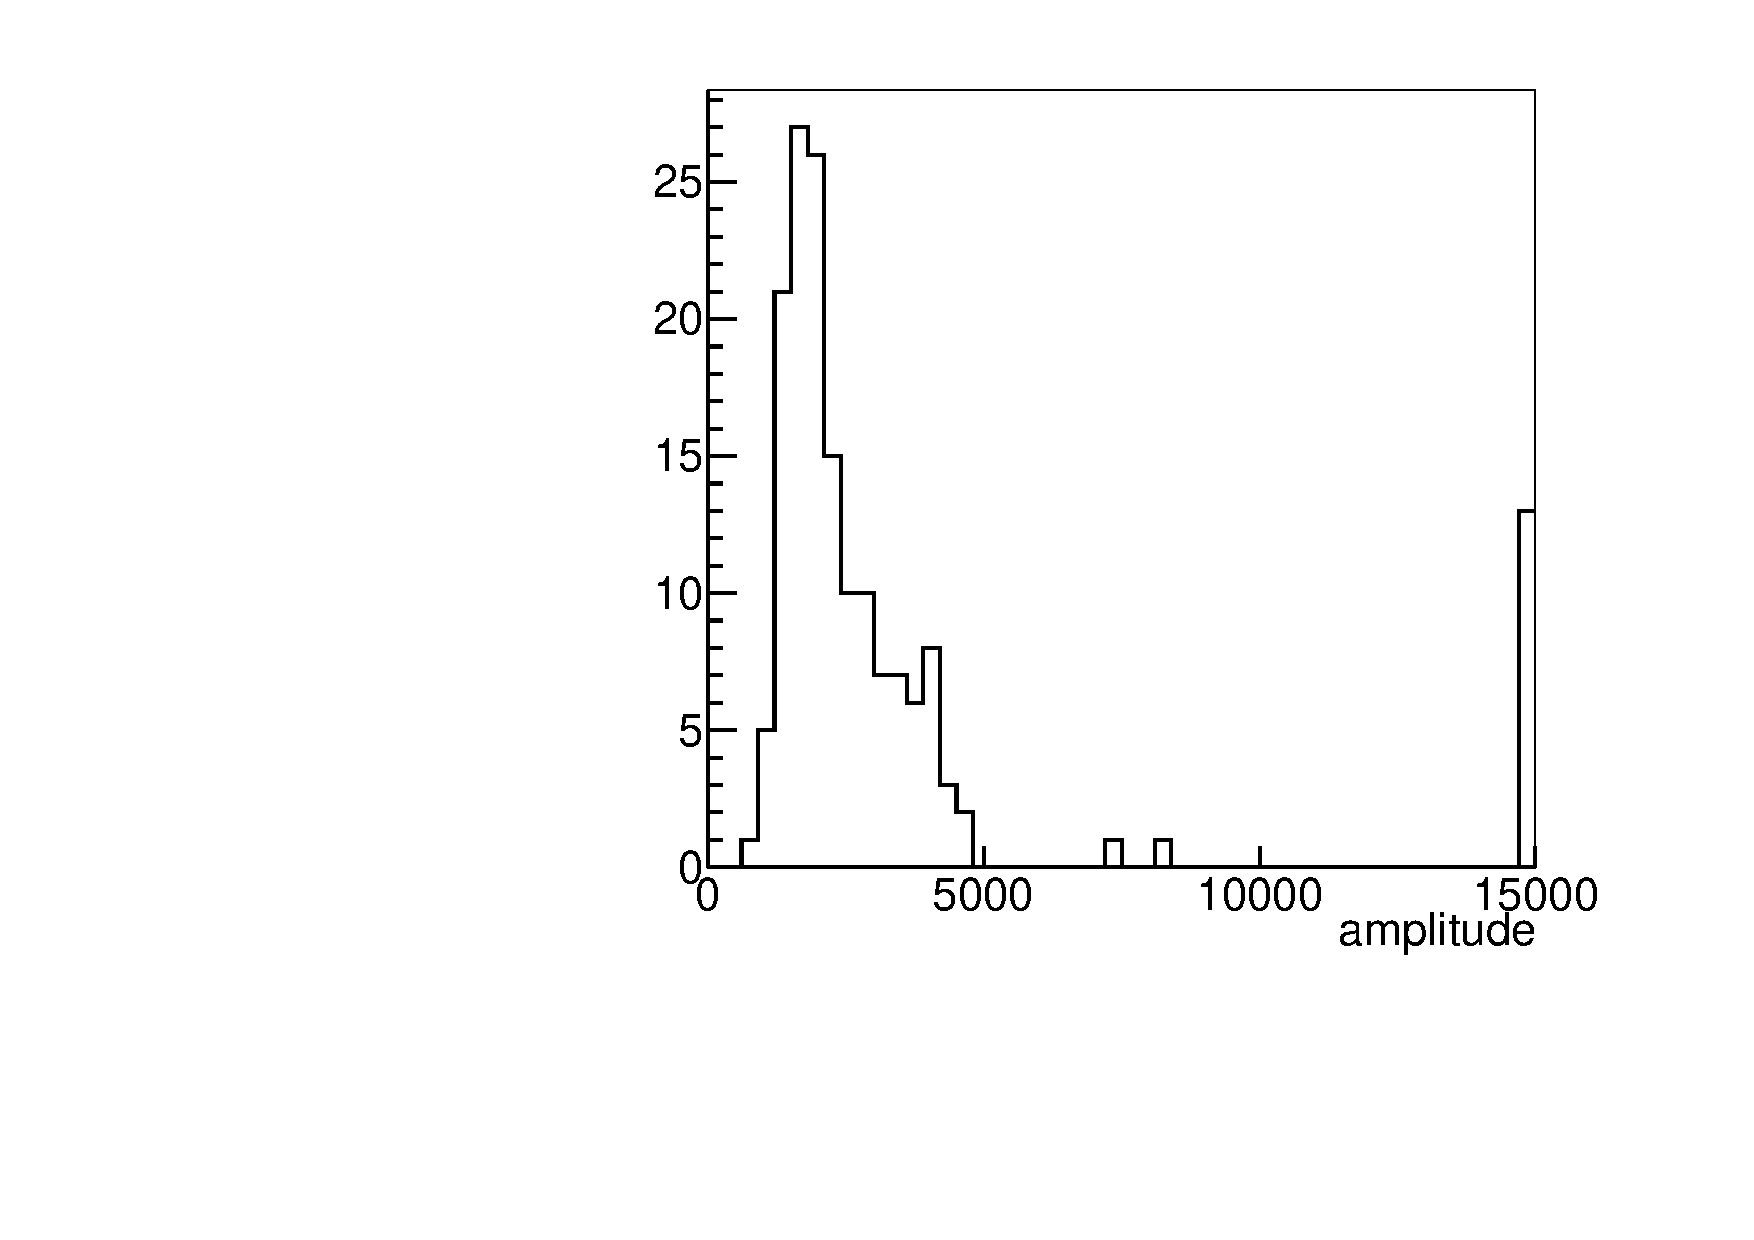
\includegraphics[width=0.3\textwidth]{Reconstruction/Figures/spikes/narrow_largealpha_amplitude.pdf}
v    \caption{
      Seed crystal pulse amplitude distributions of physical wide clusters (left), narrow clusters with $\alpha < 0.9$ (center), and narrow clusters with $\alpha > 0.9$ (right).
    }
    \label{fig:spike_amplitudes}
  \end{center}
\end{figure}

In the $\alpha$--$\beta$ parameter space, seed rec hits of wide clusters concentrate around $(\alpha, \beta) \sim (1.1, 1.7)$, while spike-like hits populate the region $\alpha < 0.9$ as shown in Figure~\ref{fig:spike_alphabeta}.
In fact, the pulse amplitude distribution of narrow-cluster seeds with $\alpha > 0.9$ is unlike that of the narrow-cluster seeds with $\alpha < 0.9$, and resembles the amplitude distribution of wide-cluster seeds shown in Figure~\ref{fig:spike_amplitudes}.
This suggests that the population $\alpha > 0.9$ correspond to the clusters of physical, prompt photons.
It then follows that spike hits can be regarded to exclusively have sharp pulse shapes.

\chapter{The Monophoton Analysis}
\label{chap:analysis}

The main event.

\section{Event Selection}
\label{sec:event_selection}

\section{Irreducible backgrounds}
\label{sec:irreducible}

\begin{figure}[htbp]
  \centering
    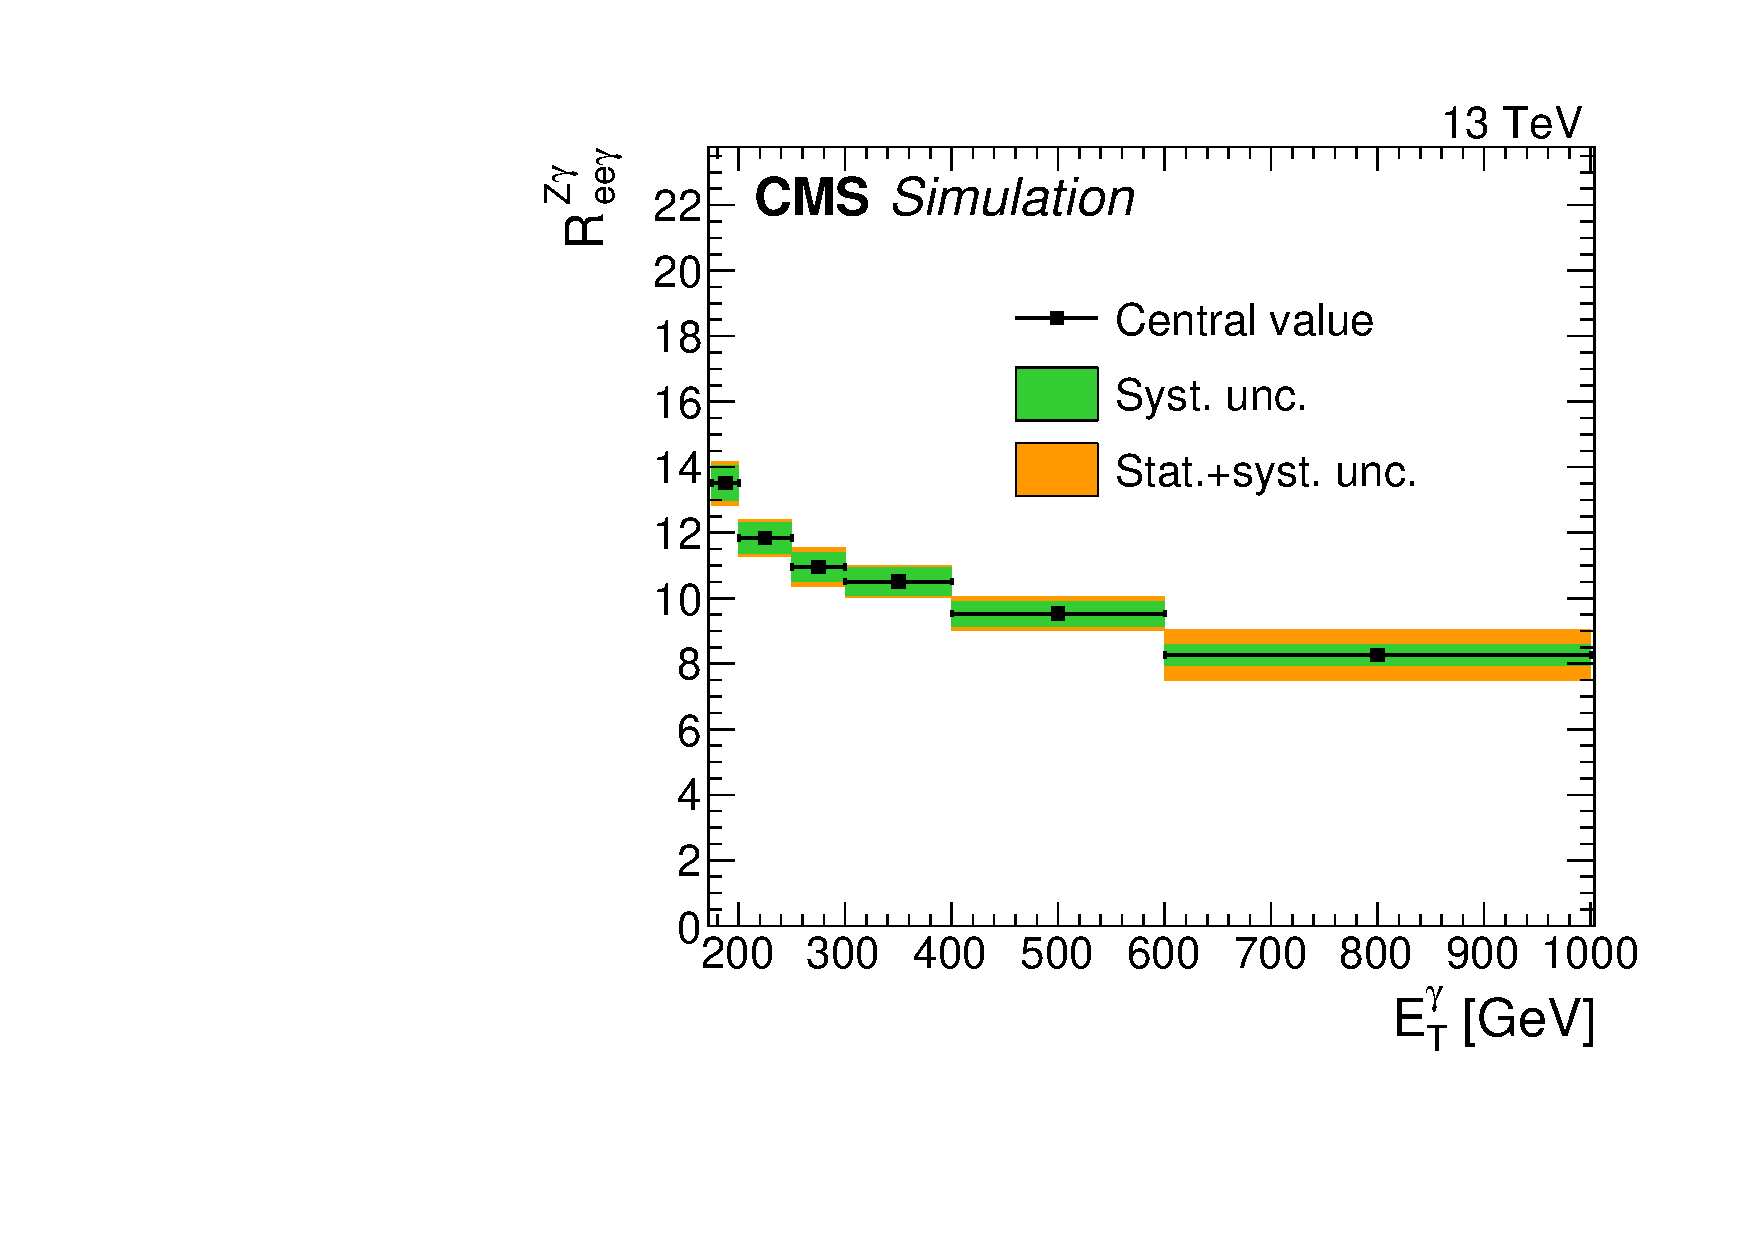
\includegraphics[width=0.49\textwidth]{Analysis/Figures/RZee.pdf}
    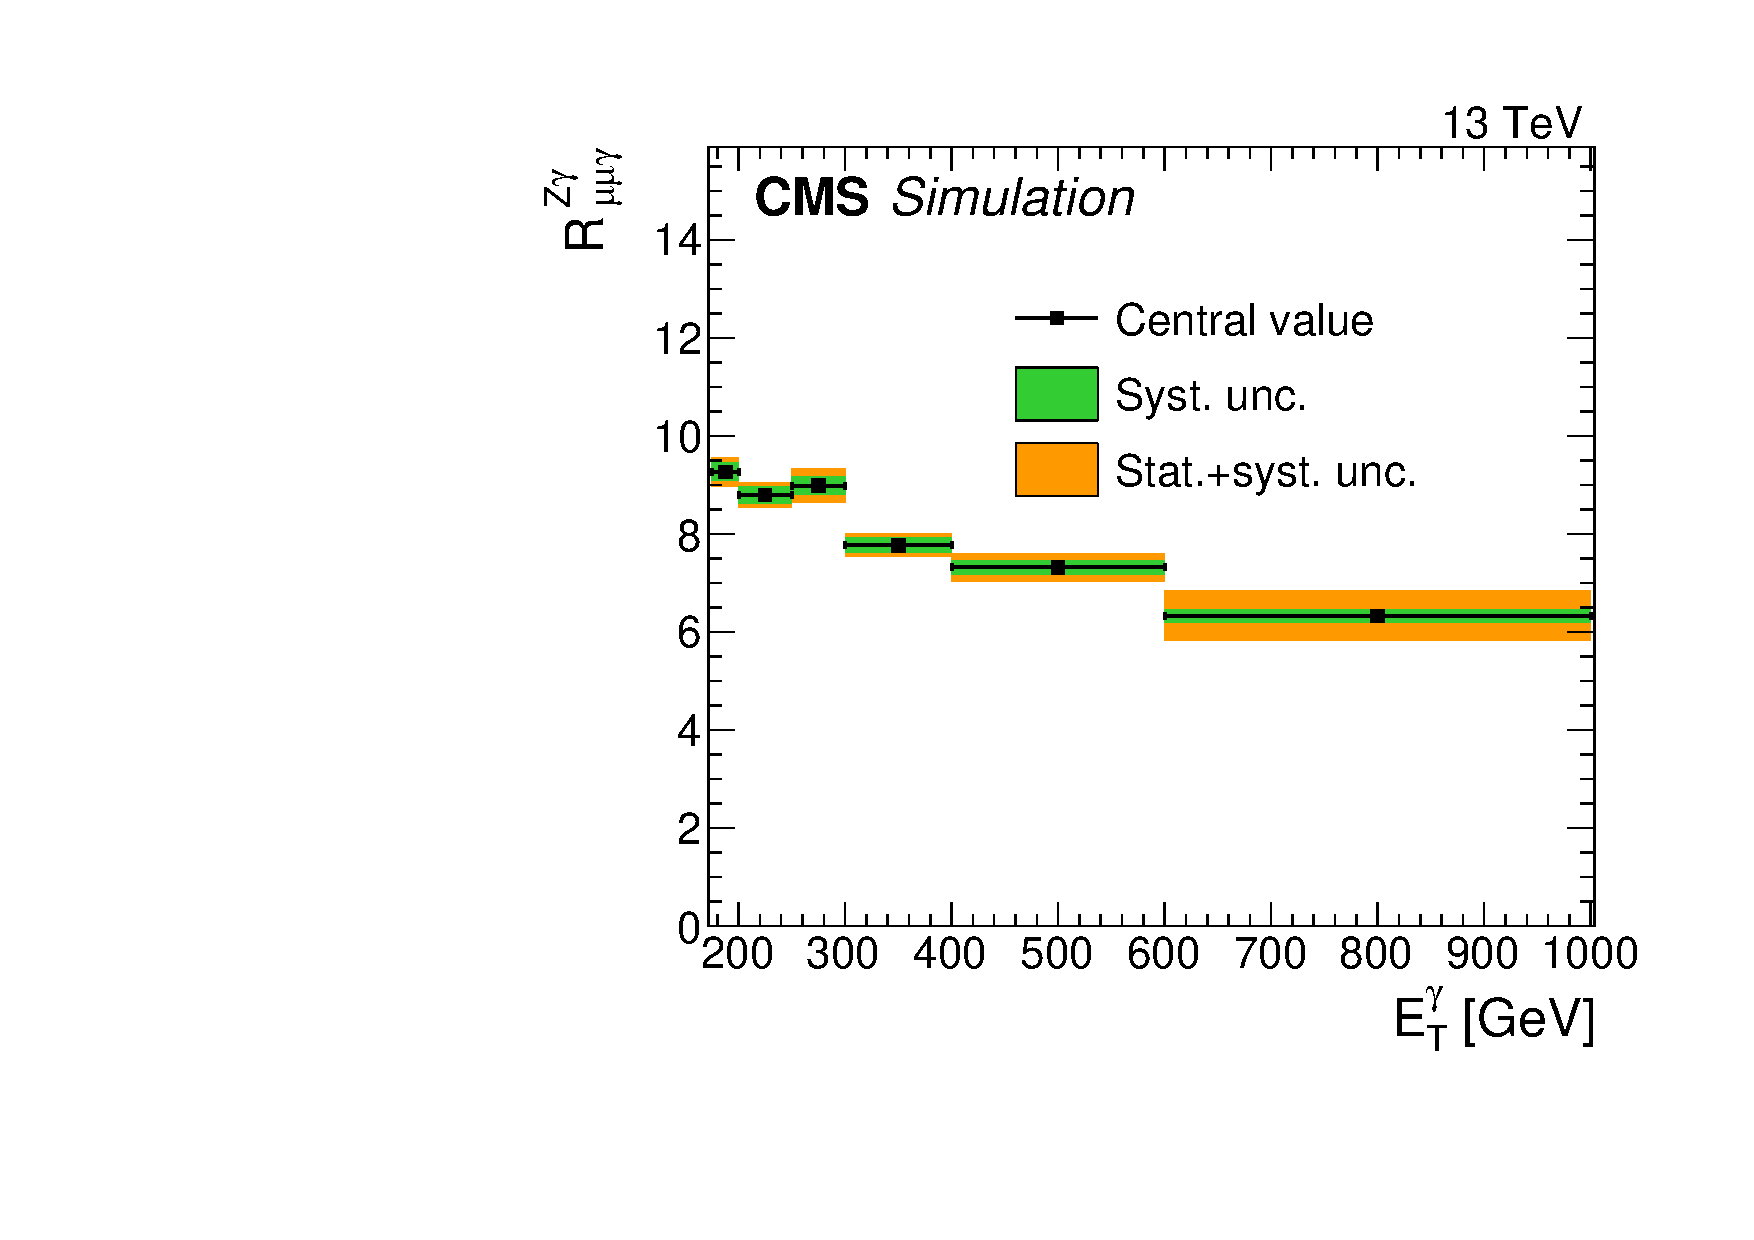
\includegraphics[width=0.49\textwidth]{Analysis/Figures/RZmm.pdf}
    \caption{
      Transfer factors \RZee\ (left) and \RZmm\ (right). 
      The uncertainty bands in green (inner) and orange (outer) show the systematic uncertainty, and the combination of systematic and statistical uncertainty arising from limited MC sample size, respectively. 
      The systematic uncertainties considered are the uncertainties in the data-to-simulation correction factors $\rho$ for the lepton identification efficiencies.
    }
    \label{fig:tf_z}
\end{figure}

Using the transfer factor \RZll, the total estimated event yield \Tll\ in each dilepton control region in the $i^\mathrm{th}$ bin of the \ETg\ distribution can be expressed as
\begin{equation}
  \Tll[,i] = \frac{\NZg[i]}{\RZll[,i]} + b_{\ell\ell\Pgg,i},
\end{equation}
where \NZg\ is the number of \zinvg\ events in the combined signal regions and $b_{\ell\ell\Pgg}$ is the predicted contribution from other background sources in the dilepton control region, namely \ttg, VV\Pgg, and misidentified hadrons. 
The subscript $i$ indicates that the quantities are evaluated in bin $i$ of the \ETg\ distribution.

\begin{figure}[htbp]
  \centering
    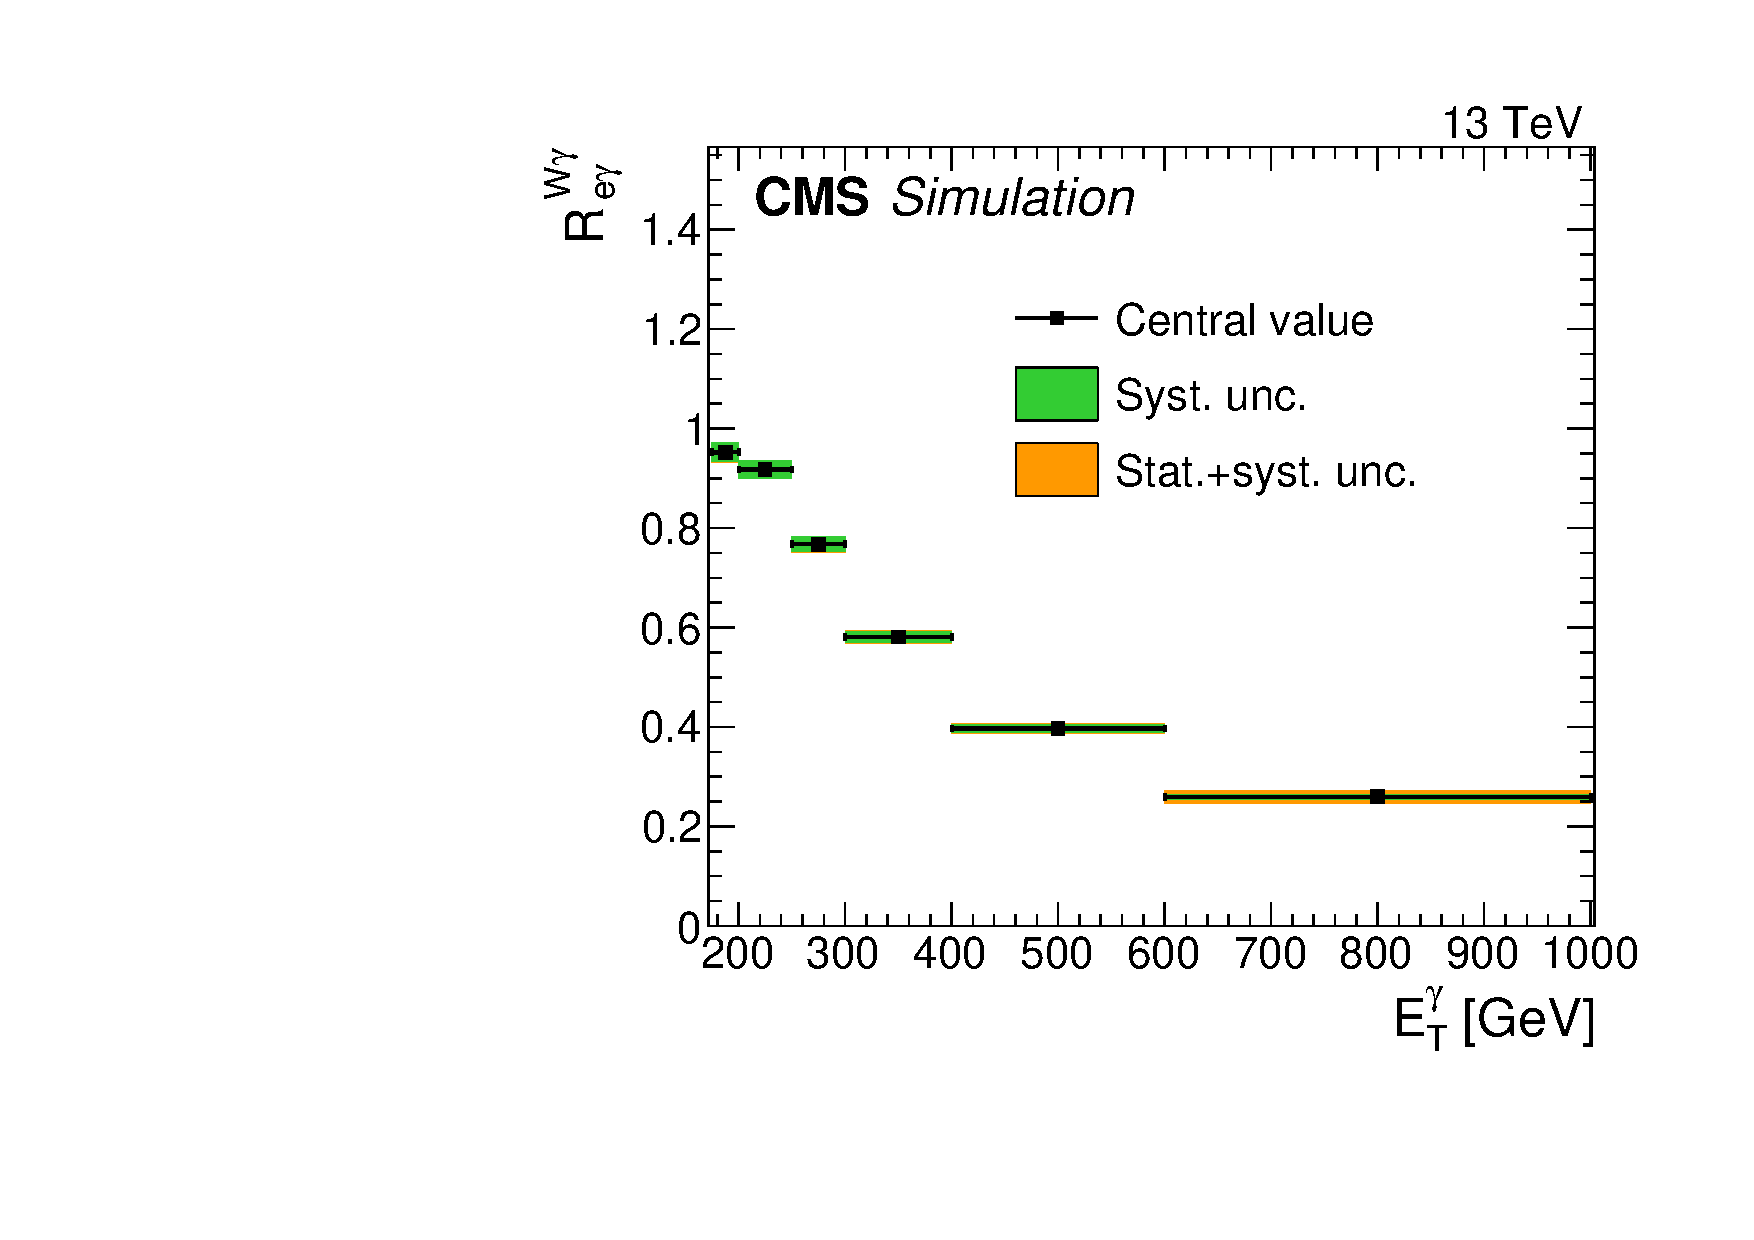
\includegraphics[width=0.49\textwidth]{Analysis/Figures/RWe.pdf}
    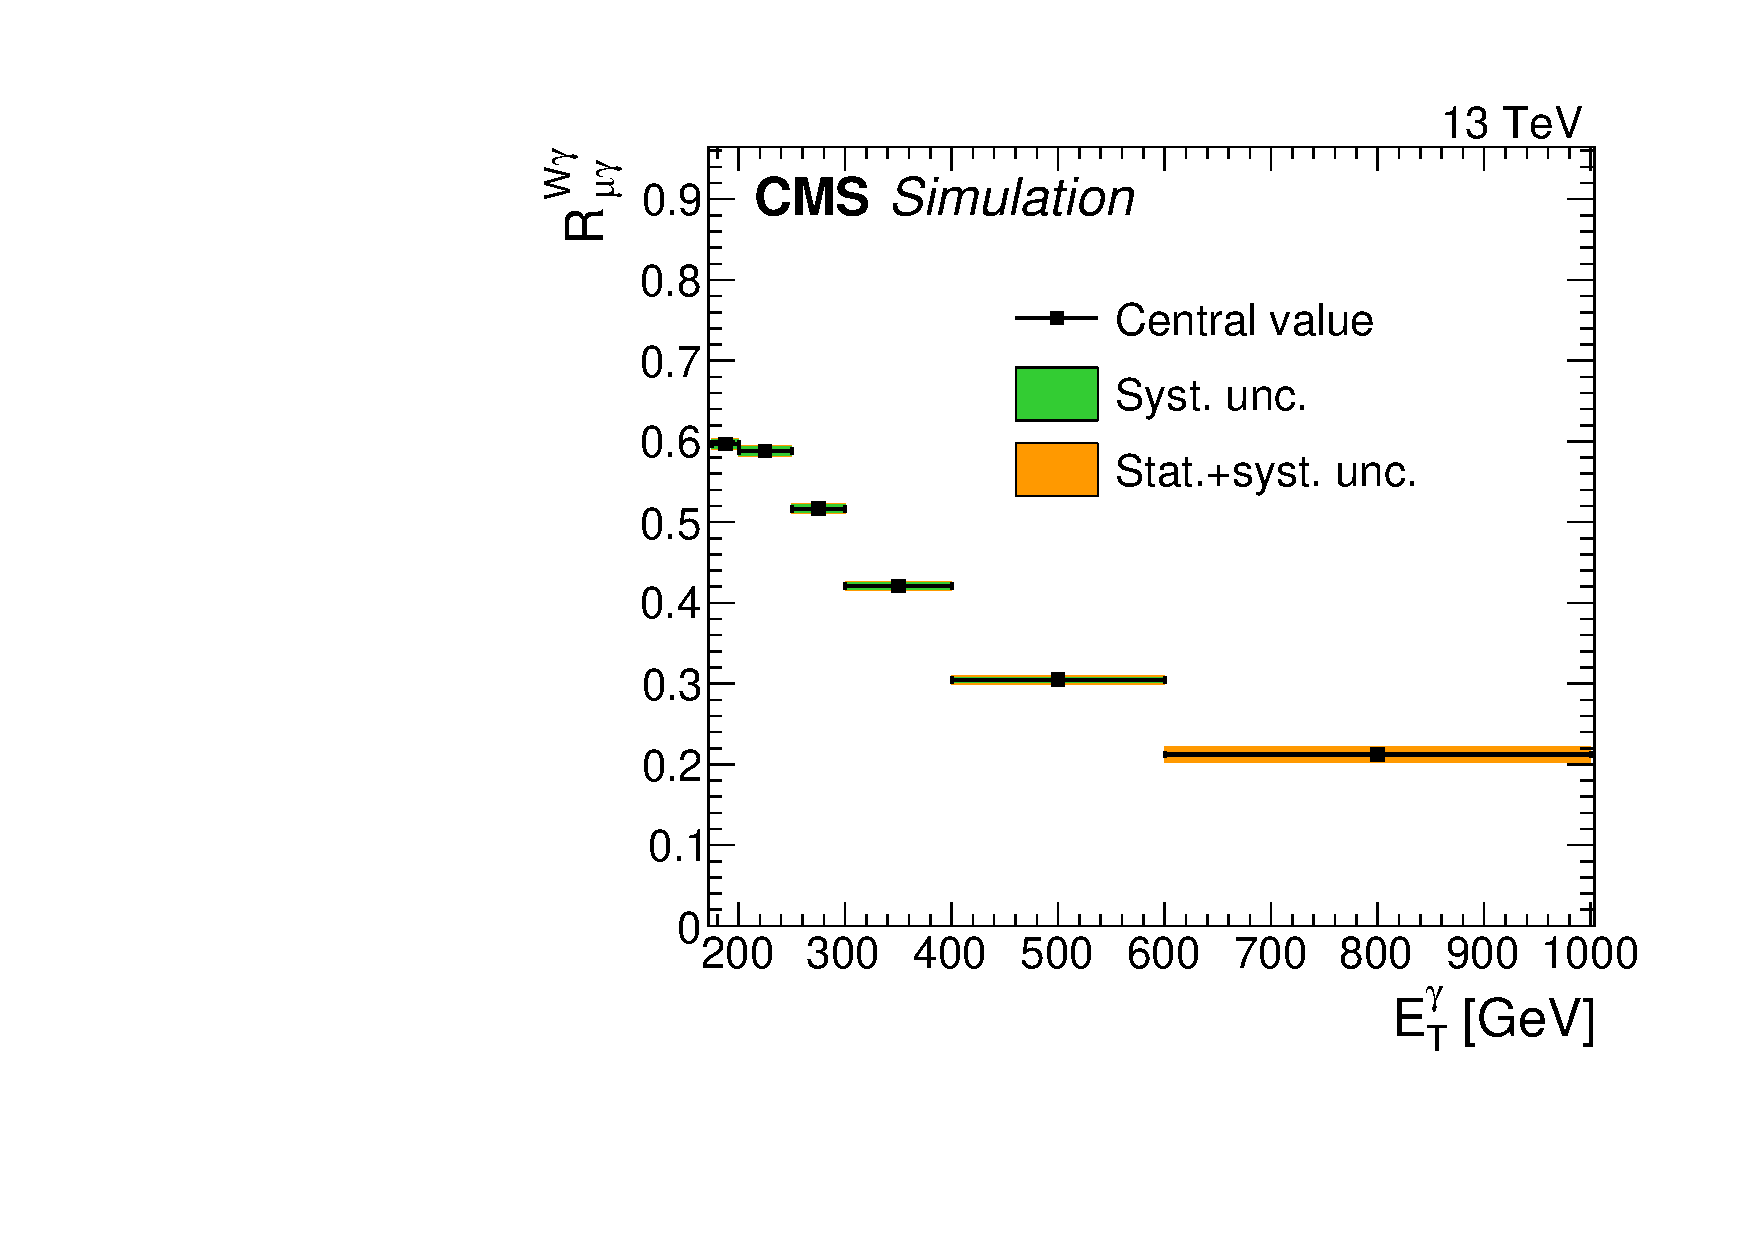
\includegraphics[width=0.49\textwidth]{Analysis/Figures/RWm.pdf}
    \caption{
      Transfer factors \RWe\ (left) and \RWm\ (right). 
      The uncertainty bands in green (inner) and orange (outer) show the systematic uncertainty, and the combination of systematic and statistical uncertainty arising from limited MC sample size, respectively. 
      The systematic uncertainties considered are the uncertainties in the data-to-simulation correction factors $\rho$ for the lepton identification efficiencies.
    }
    \label{fig:tf_w}
\end{figure}

\begin{figure}[htbp]
  \centering
    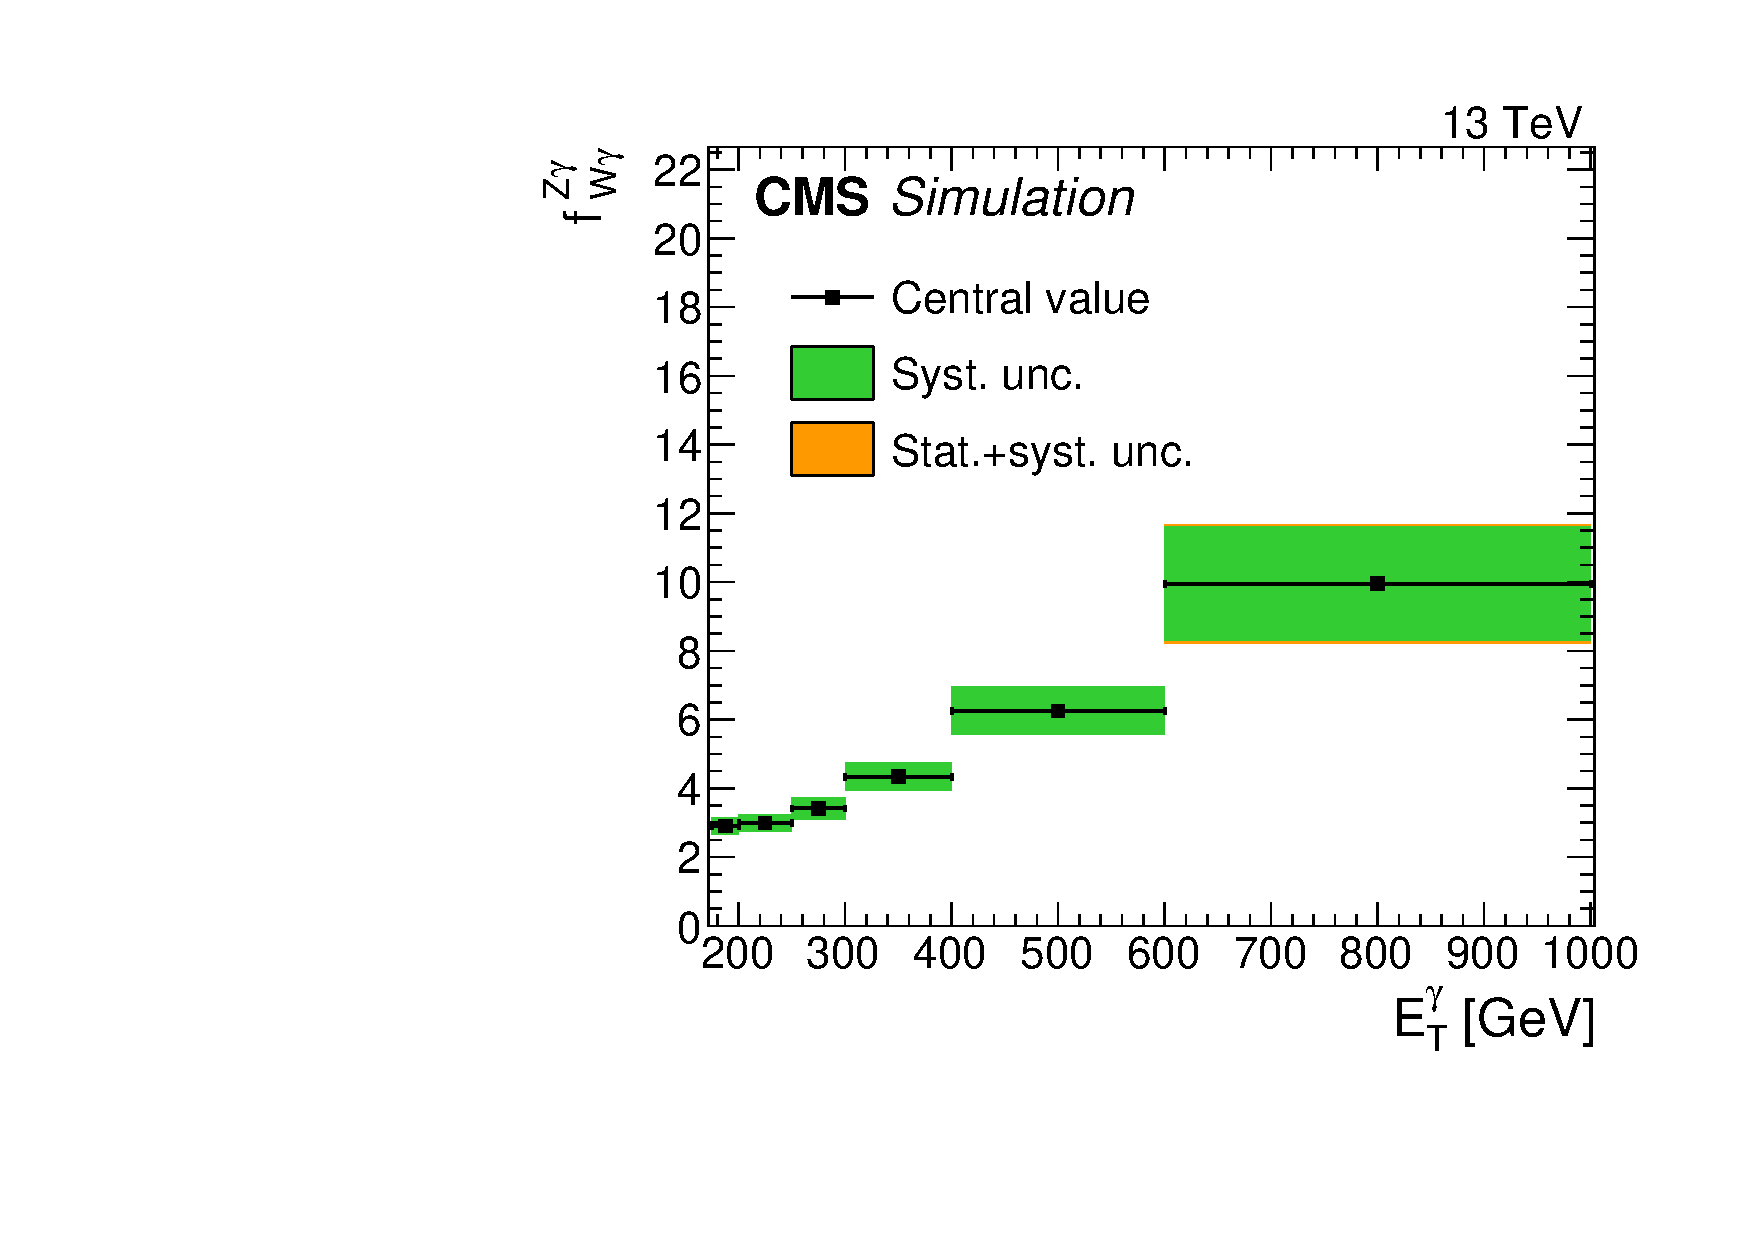
\includegraphics[width=0.49\textwidth]{Analysis/Figures/fZW.pdf}
    \caption{
      Transfer factor \fZW. 
      The uncertainty bands in green (inner) and orange (outer) show the systematic uncertainty, and the combination of systematic and statistical uncertainty arising from limited MC sample size, respectively. 
      The systematic uncertainties considered are the uncertainties from higher-order theoretical corrections.
    }
    \label{fig:tf_wz}
\end{figure}

Using \RWl\ and \fZW, the total estimated event yield \Tl\ in each single-lepton control region in the $i^\mathrm{th}$ bin of the \ETg\ distribution can be expressed as
\begin{equation}
  \Tl[,i] = \frac{\NZg[i]}{\RWl[,i]\fZW[,i]} + b_{\ell\Pgg,i},
\end{equation}
where $b_{\ell\Pgg}$ is the predicted contribution from other background sources in the single-lepton regions, namely misidentified electrons and hadrons and other minor SM processes.

\section{Misidentified backgrounds}
\label{sec:misidentified}

\subsection{Electrons}
\label{sec:efake}

\subsection{Hadrons}
\label{sec:hfake}

\section{Non-collision backgrounds}
\label{non-collision}

\subsection{Spikes}
\label{sec:spikes}

\subsection{Beam halo}
\label{sec:beam_halo}

The splitting of the signal region can be thought of as a two-bin fit. 
Collision processes occupy the relative fractions of phase space in the horizontal ($H$) and vertical ($V$) signal regions, $C_{H} = 1/\pi$ and $C_{V} = (\pi-1)/\pi$, respectively. 
The corresponding fractions for beam halo events are determined by selecting a halo-enriched sample where the halo identification is inverted. 
Thus, a fit of the two signal regions provides an estimate of the overall normalization of the beam halo background, denoted $h$. 
The \ETg\ dependence of the halo background is encoded in \nhalo[,i], the unit-normalized beam halo prediction in the $i^\mathrm{th}$ bin of the signal region $K \in \{H,V\}$.
Using the notation introduced in Section~\ref{sec:irreducible}, the total estimated background \TK\ in the two signal regions are
\begin{equation}
\begin{aligned}
  \TK[,i] & = C_{K} (\NZg[i] + \NWg[i]) + h \nhalo[,i] + C_{K} b_{K,i} \\
          & = C_{K} (1 + {\fZW[i]}^{-1}) \NZg[i] + h \nhalo[,i] + C_{K} b_{K,i},
\end{aligned}
\end{equation}
where $b_{K,i}$ is the total contribution to bin $i$ of region $K$ from electron and hadron misidentification, ECAL spikes, and other minor SM background processes.

\section{Statistical Interpretation}
\label{sec:interpretation}

Free parameters of the fit are the yield of \zinvg\ background in each bin of the signal regions (\NZg[i]) and the overall normalization of the beam halo background ($h$). 
Bin-by-bin yields of \wlng\ and \zllg\ samples in all regions are related to the yield of \zinvg\ through the MC prediction through the transfer factors defined in Section~\ref{sec:irreducible}. 
The transfer factors are allowed to shift within the aforementioned theoretical and experimental uncertainties.

The background-only likelihood that is maximized in the fit is
\begin{equation}
\begin{aligned}
  \mathcal{L} & = \prod_{i} \left\{ \mathcal{L_{\text{signal}}} \times \mathcal{L_{\text{single-lepton}}} \times \mathcal{L_{\text{dilepton}}} \right\} \times \mathcal{L_{\text{nuisances}}} \\
  & = \prod_{i} \left\{
    \prod_{K=H,V} \mathcal{P}\left( d_{K, i} \left| \TK[,i] (\vec{\theta} \right.) \right) \times \prod_{\ell=\Pe,\Pgm} \mathcal{P}\left( d_{\ell\Pgg, i} \left| \Tl[,i] (\vec{\theta}) \right. \right)
    \times \prod_{\ell=\Pe,\Pgm} \mathcal{P}\left( d_{\ell\ell\Pgg, i} \left| \Tll[,i] (\vec{\theta}) \right. \right)
    \right\}  \times \prod_{j} \mathcal{N}(\theta_j) \\
  & = \prod_{i} \left\{
  \begin{gathered}
    \prod\limits_{K=H,V} \mathcal{P}\biggl( d_{K, i} \biggl| \left(1 + {\fZW[,i]}^{-1}(\vec{\theta})\right) C_{K} \NZg[i] + h \nhalo[,i](\vec{\theta}) + C_{K} b_{K, i}(\vec{\theta}) \biggr. \biggr) \\
    \times \prod\limits_{\ell=\Pe,\Pgm} \mathcal{P}\biggl( d_{\ell\Pgg, i} \biggl| \frac{\NZg[i]}{\RWl[,i](\vec{\theta}) \fZW[,i] (\vec{\theta})} + b_{\ell\Pgg, i}(\vec{\theta}) \biggr. \biggr) \\
    \times \prod\limits_{\ell=\Pe,\Pgm} \mathcal{P}\biggl( d_{\ell\ell\Pgg, i} \biggl| \frac{\NZg[i]}{\RZll[,i](\vec{\theta})} + b_{\ell\ell\Pgg, i}(\vec{\theta}) \biggr. \biggr)
  \end{gathered} \right\}
  \times \prod_{j} \mathcal{N}(\theta_j),
\end{aligned}
\end{equation}
following the notation introduced in Section~\ref{sec:irreducible}, and where $\mathcal{P}
(n\vert\lambda)$ is the Poisson probability of $n$ for mean $\lambda$, $\mathcal{N}$ denotes the unit normal distribution, and $d_{X,i}$ is the observed number of events in bin i of region X.
Systematic uncertainties are treated as nuisance parameters in the fit and are represented by
$\vec{\theta}$.
Each quantity $Q_{j}$ with a nominal value $\overline{Q}_{j}$ and a standard deviation of the systematic uncertainty $\sigma_{j}$ appears in the likelihood function as $\overline{Q}_{j}\exp(\sigma_{j}\theta_{j})$.

\section{Results}
\label{sec:results}

\subsection{Pre-fit and post-fit distributions}
\label{subsec:distributions}

\begin{figure}[htbp]
  \centering
    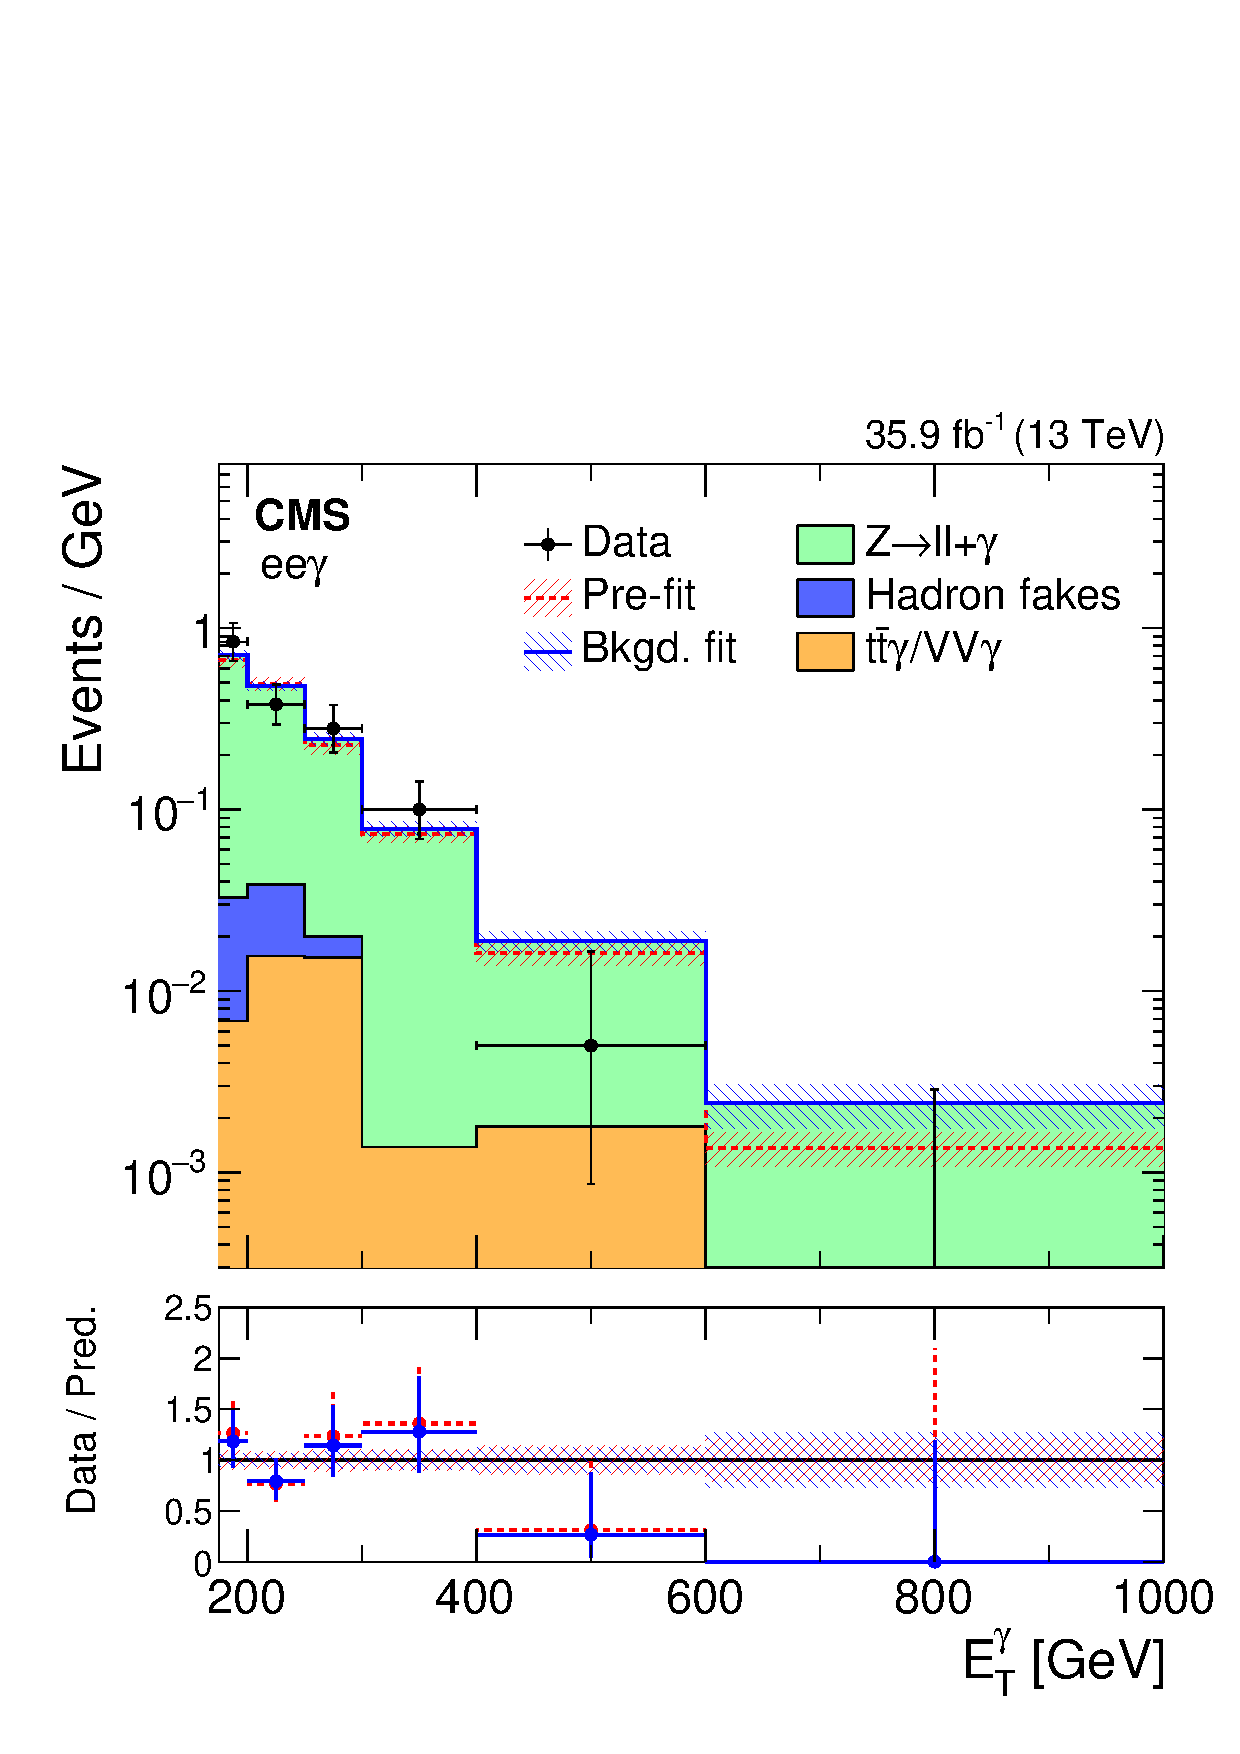
\includegraphics[width=0.45\textwidth]{Analysis/Figures/bonly_diel.pdf}
    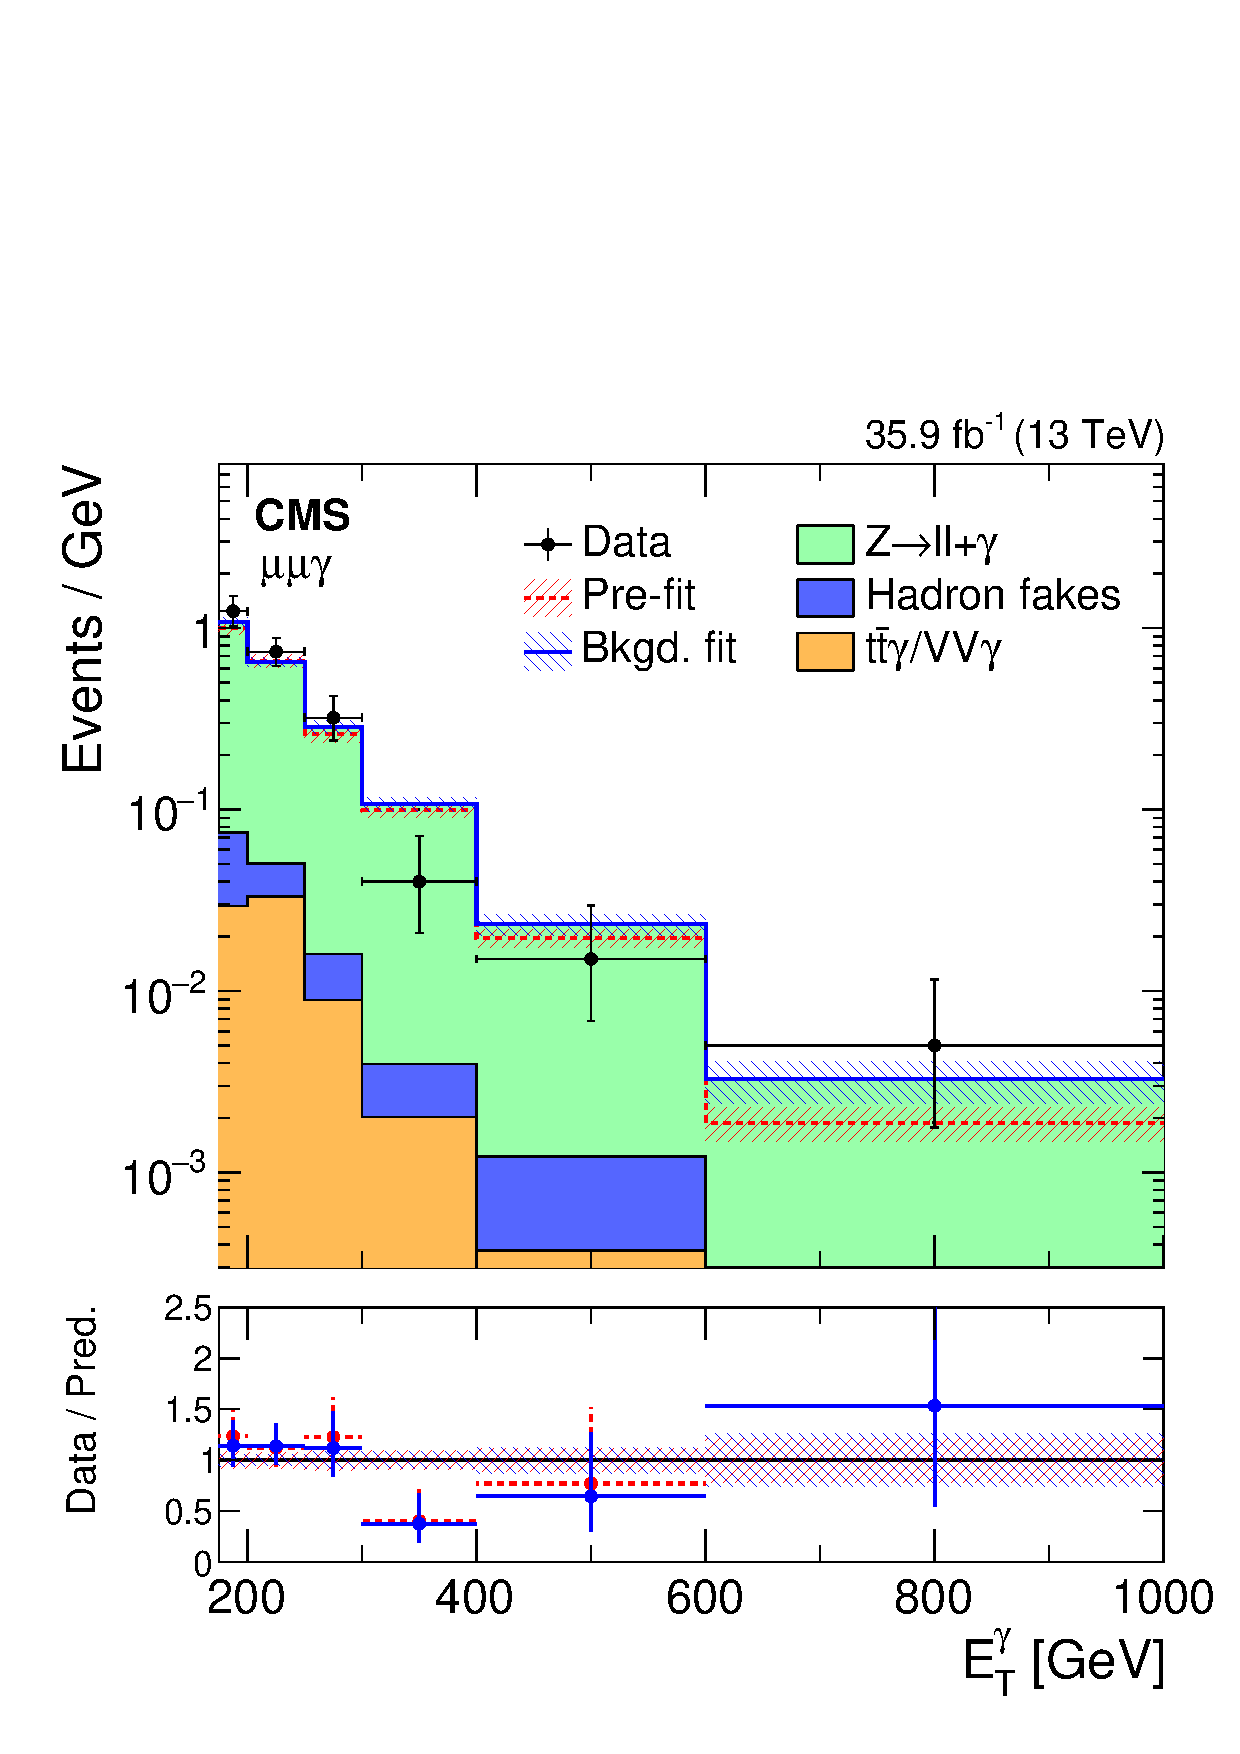
\includegraphics[width=0.45\textwidth]{Analysis/Figures/bonly_dimu.pdf}
    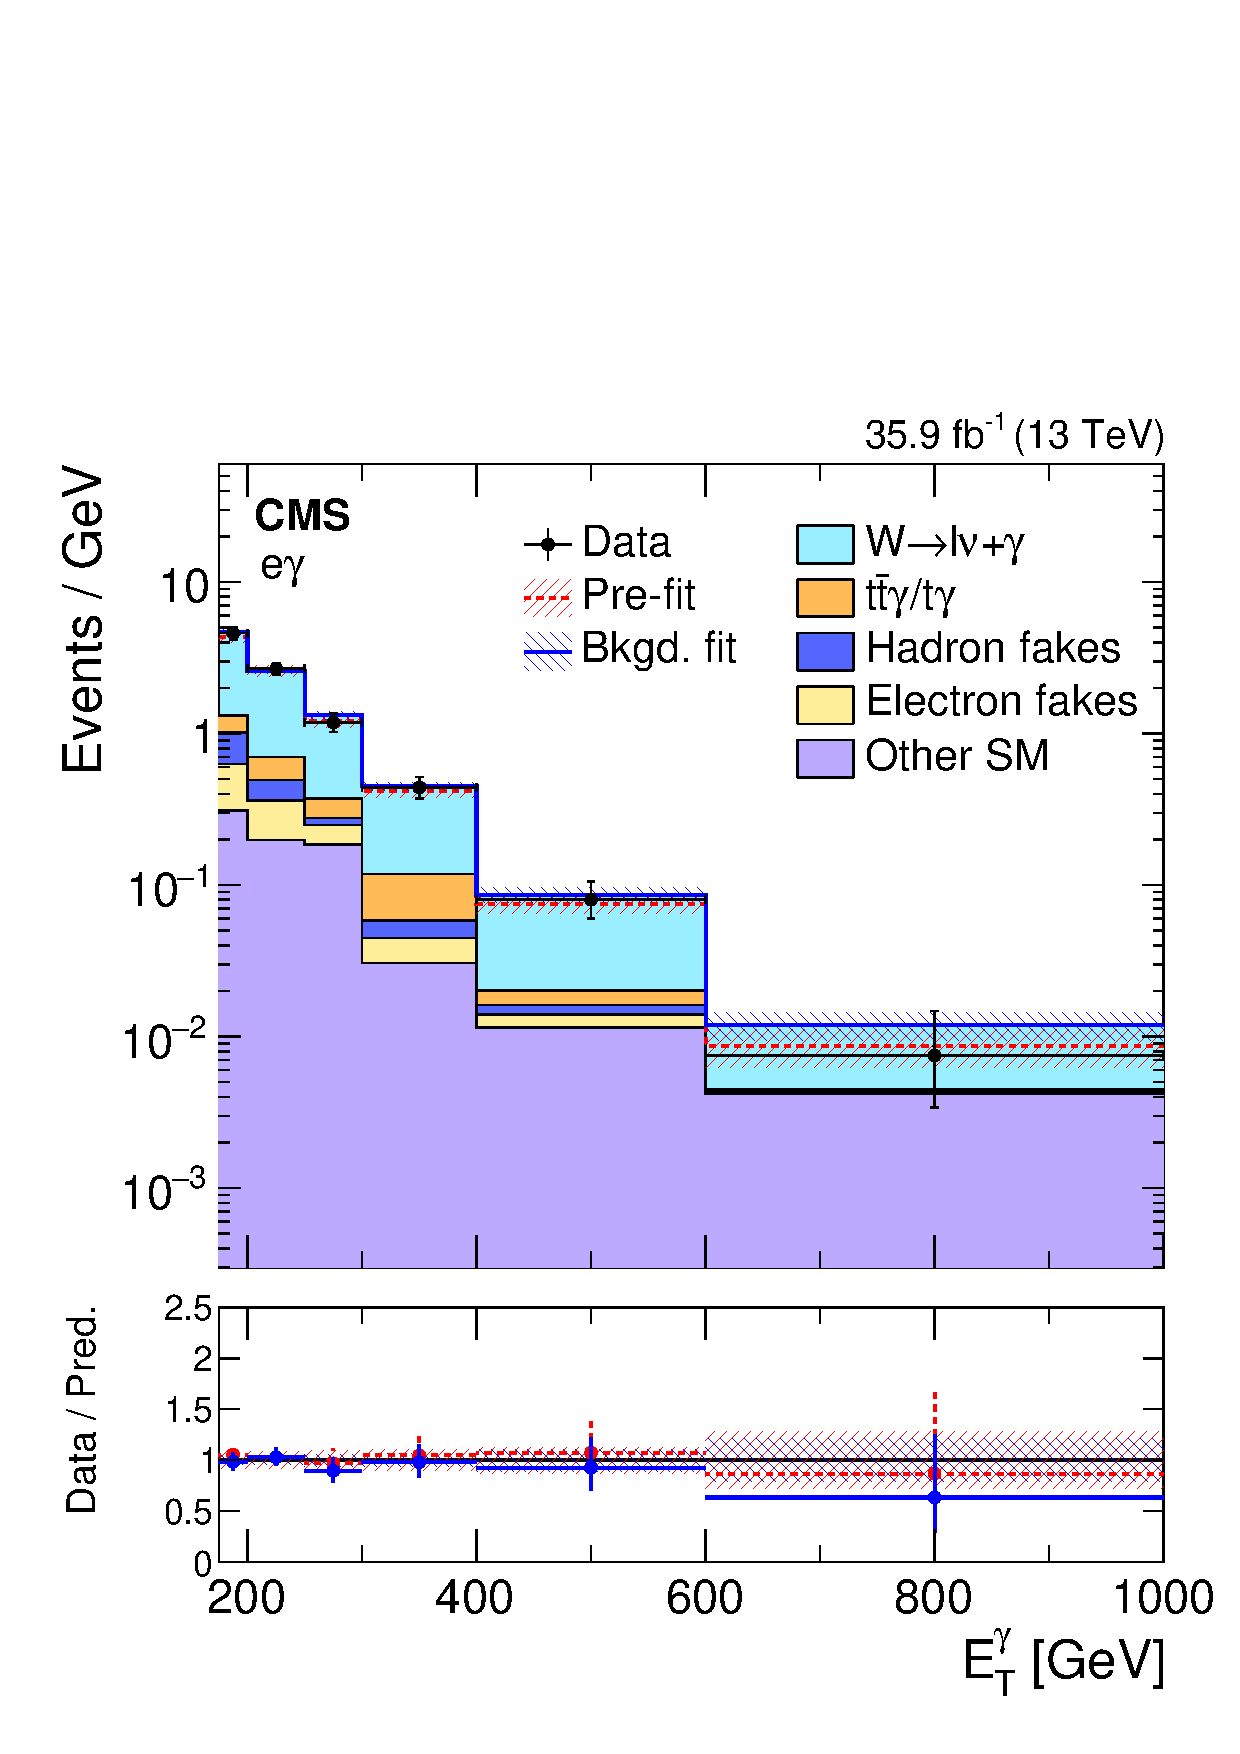
\includegraphics[width=0.45\textwidth]{Analysis/Figures/bonly_monoel.pdf}
    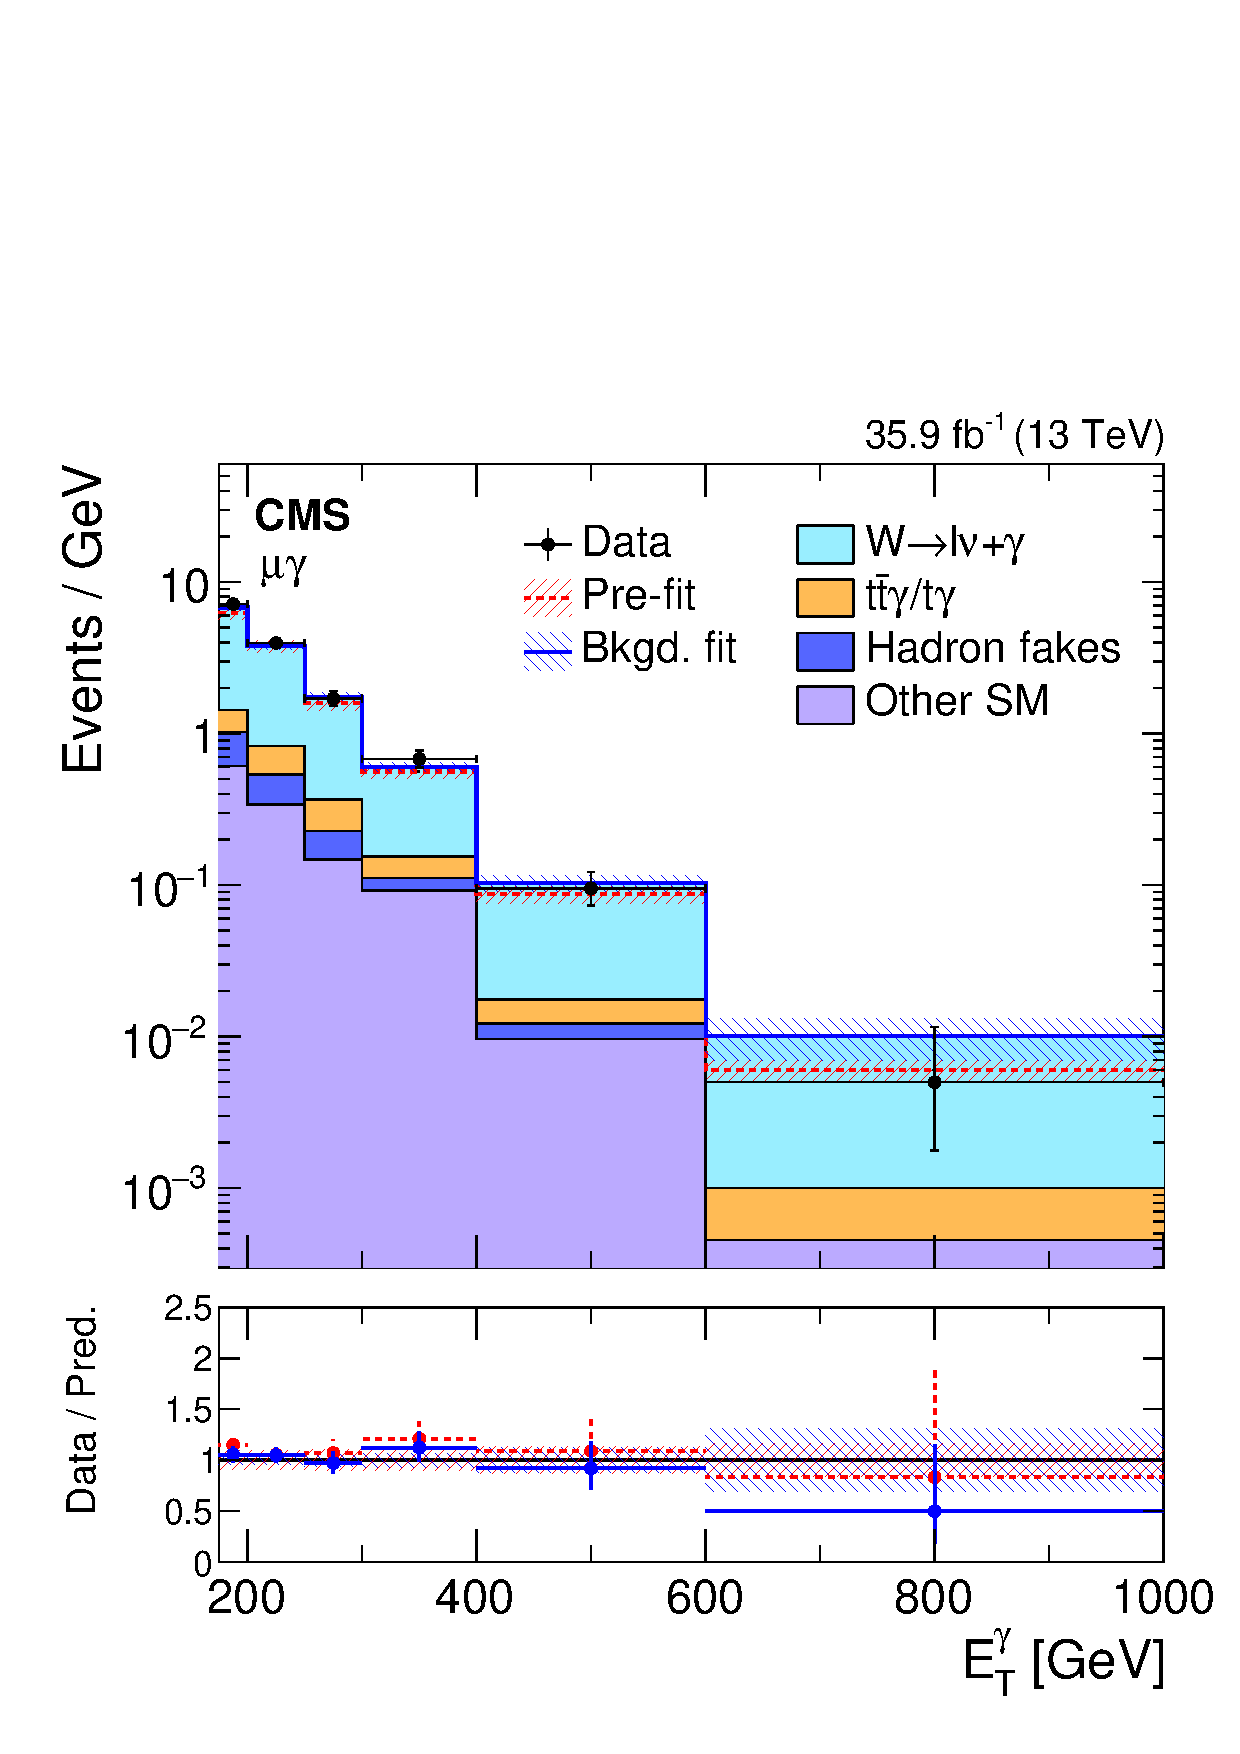
\includegraphics[width=0.45\textwidth]{Analysis/Figures/bonly_monomu.pdf}
    \caption{
      Comparison between data and MC simulation in the four control regions: 
      \Pe\Pe\Pgg\ (upper left), 
      \Pgm\Pgm\Pgg\ (upper right), 
      \Pe\Pgg\ (lower left), 
      \Pgm\Pgg\ (lower right) 
      before and after performing the simultaneous fit across all the control samples and signal region, and assuming absence of any signal.
      The last bin of the distribution includes all events with $\ETg > 1000\GeV$. 
      The ratios of data with the pre-fit background prediction (red dashed) and post-fit background prediction (blue solid) are shown in the lower panels. 
      The bands in the lower panels show the post-fit uncertainty after combining all the systematic uncertainties.
}
    \label{fig:postfitCR}
\end{figure}

\begin{figure}[htbp]
  \centering
    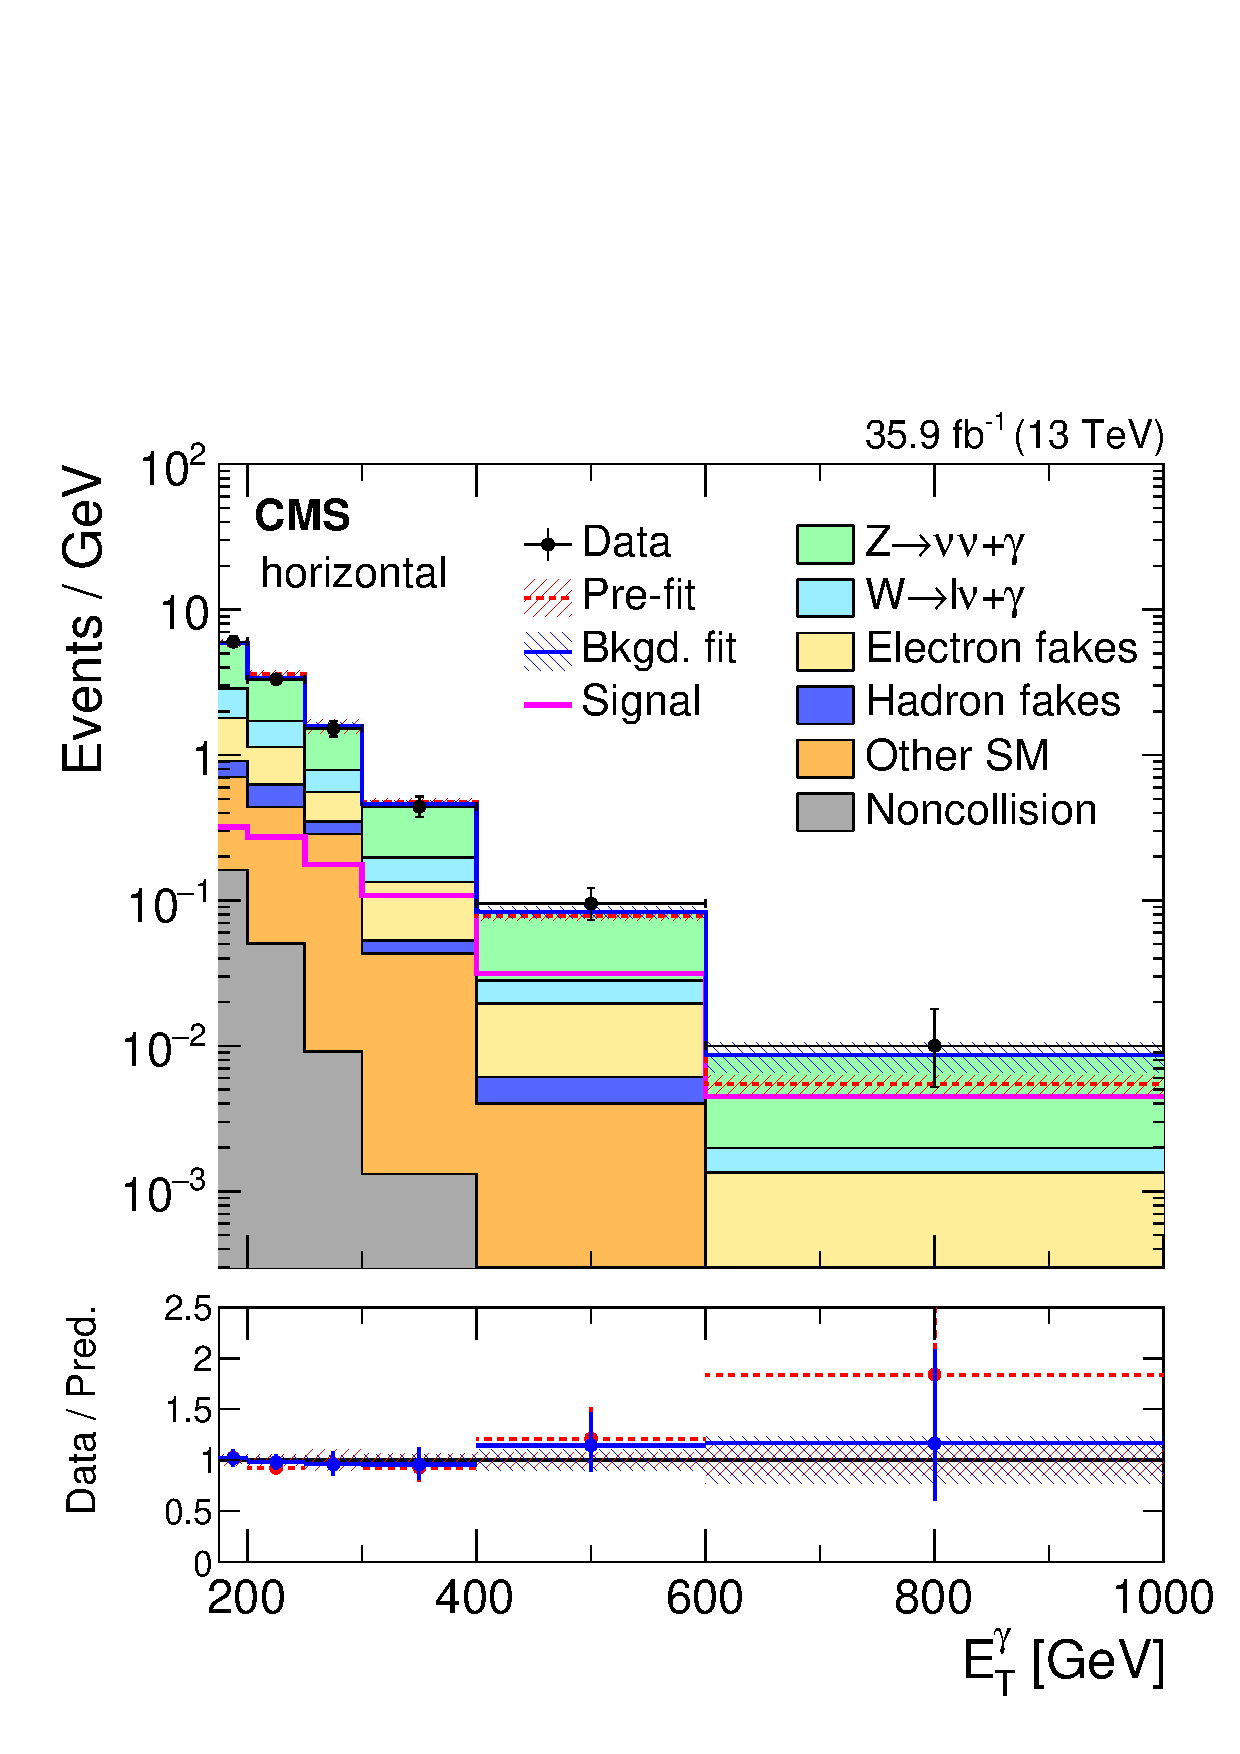
\includegraphics[width=0.45\textwidth]{Analysis/Figures/bonly_horizontal.pdf}
    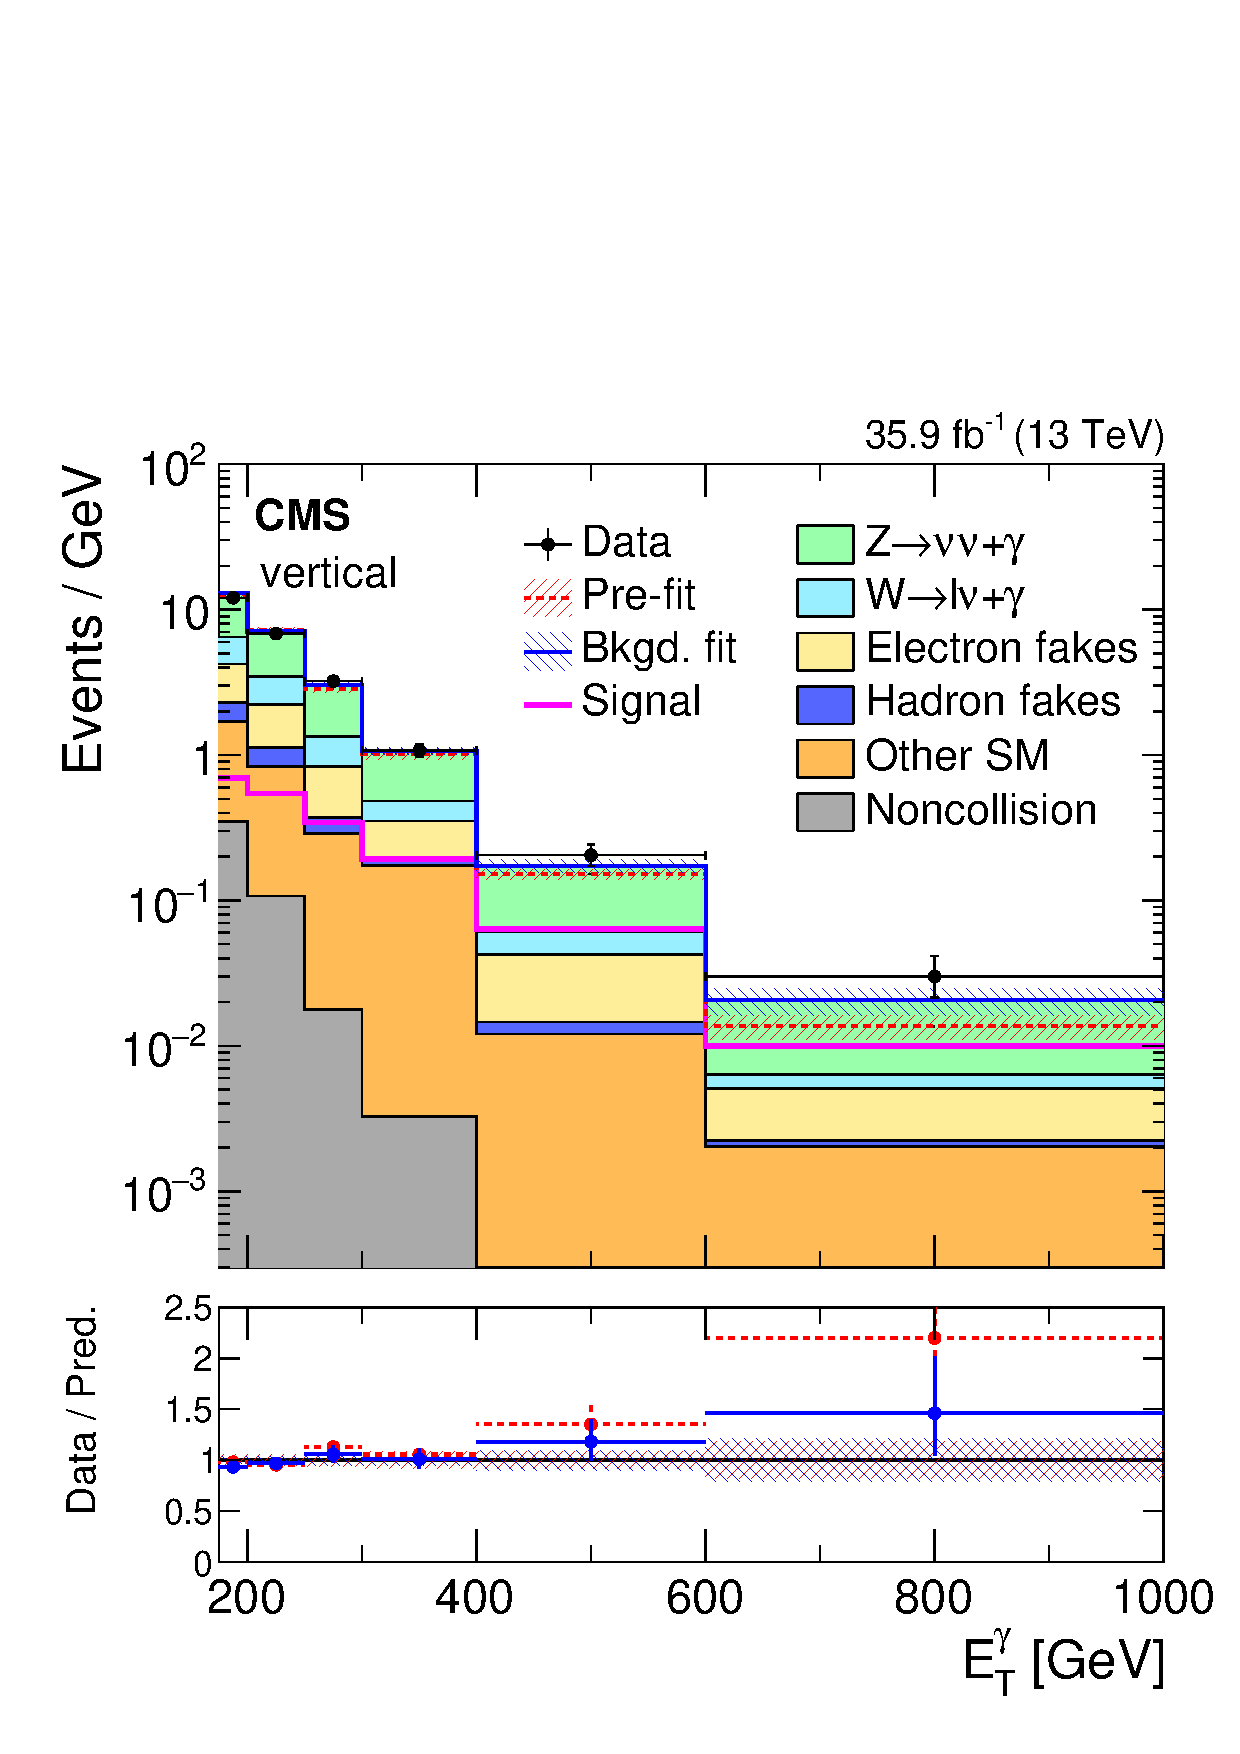
\includegraphics[width=0.45\textwidth]{Analysis/Figures/bonly_vertical.pdf}
    \caption{
      Observed \ETg\ distributions in the horizontal (left) and vertical (right) signal regions compared with the post-fit background expectations for various SM processes.
      The last bin of the distribution includes all events with $\ETg > 1000\GeV$. 
      The expected background distributions are evaluated after performing a combined fit to the data in all the control samples and the signal region. 
      The ratios of data with the pre-fit background prediction (red dashed) and post-fit background prediction (blue solid) are shown in the lower panels. 
      The bands in the lower panels show the post-fit uncertainty after combining all the systematic uncertainties. 
      The expected signal distribution from a 1\TeV vector mediator decaying to 1\GeV DM particles is overlaid.
    }
    \label{fig:postfitSR}
\end{figure}

Figure~\ref{fig:postfitCR} shows the observed \ETg\ distributionsin the four control regions compared with the results from simulations before and after performing the simultaneous fit across all the control samples and signal region, and assuming absence of any signal.
Figure~\ref{fig:postfitSR} shows the observed \ETg\ distributions in the horizontal and vertical signal regions compared with the results from simulations before and after performing a combined fit to the data in all the control samples and the signal region. 
The observed distributions are in agreement with the prediction from SM and noncollision backgrounds.

\begin{table}[htbp]
\centering
\caption{Expected event yields in each \ETg\ bin for various background processes in the horizontal signal region.
         The background yields and the corresponding uncertainties are obtained after performing a combined fit to data in all the control samples, excluding data in the signal region.
         The observed event yields in the horizontal signal region are also reported.}
\label{tab:yield_mask_horizontal}
\begin{tabular}{ lcccccc }
\hline
\rule[-1.2ex]{0pt}{3.8ex}\ETg~[\GeVns{}]      &         [175,  200] &         [200,  250] &         [250,  300] &         [300,  400] &         [400,  600] &         [600, 1000] \\
\hline
$\PZ\Pgg$        & $  81.2 \pm   8.0 $ & $  88.2 \pm   8.4 $ & $  38.8 \pm   4.8 $ & $  26.8 \pm   3.7 $ & $   8.8 \pm   1.9 $ & $   1.4 \pm   0.7 $ \\
$\PW\Pgg$        & $  27.9 \pm   3.7 $ & $  29.9 \pm   3.9 $ & $  11.4 \pm   1.7 $ & $   6.3 \pm   1.2 $ & $   1.4 \pm   0.4 $ & $   0.1 \pm   0.1 $ \\
Misid. electrons & $  22.5 \pm   2.7 $ & $  25.7 \pm   2.7 $ & $  10.5 \pm   1.0 $ & $   8.2 \pm   0.7 $ & $   2.7 \pm   0.2 $ & $   0.5 \pm   0.0 $ \\
Misid. hadrons   & $   5.2 \pm   2.2 $ & $   9.3 \pm   1.8 $ & $   3.1 \pm   0.7 $ & $   1.0 \pm   0.3 $ & $   0.4 \pm   0.1 $ & $   0.0 \pm   0.0 $ \\
Other SM         & $  13.6 \pm   2.0 $ & $  19.6 \pm   1.3 $ & $  13.9 \pm   0.4 $ & $   4.2 \pm   0.2 $ & $   0.8 \pm   0.0 $ & $   0.1 \pm   0.0 $ \\
ECAL spikes      & $   4.3 \pm   1.3 $ & $   2.7 \pm   0.8 $ & $   0.5 \pm   0.1 $ & $   0.1 \pm   0.0 $ & $   0.0 \pm   0.0 $ & $   0.0 \pm   0.0 $ \\
Total prediction & $ 154.6 \pm   8.3 $ & $ 175.4 \pm   8.8 $ & $  78.2 \pm   5.3 $ & $  46.6 \pm   4.0 $ & $  14.1 \pm   2.1 $ & $   2.1 \pm   0.8 $ \\
Observed         & $ 150   \pm  12   $ & $ 166   \pm    13 $ & $  76.0 \pm   8.7 $ & $  44.0 \pm   6.6 $ & $  19.0 \pm   4.4 $ & $   4.0 \pm   2.0 $ \\
\hline
\end{tabular}
\end{table}

\begin{table}[htbp]
\centering
\caption{Expected event yields in each \ETg\ bin for various background processes in the vertical signal region.
         The background yields and the corresponding uncertainties are obtained after performing a combined fit to data in all the control samples, excluding data in the signal regions.
         The observed event yields in the vertical signal region are also reported.}
\label{tab:yield_mask_vertical}
\begin{tabular}{ lcccccc }
\hline
\rule[-1.2ex]{0pt}{3.8ex}\ETg~[\GeVns{}]      &         [175,  200] &         [200,  250] &         [250,  300] &         [300,  400] &         [400,  600] &         [600, 1000] \\
\hline
$\PZ\Pgg$        & $ 172   \pm    17 $ & $ 190   \pm  18   $ & $  83   \pm  10   $ & $  58.6 \pm   7.9 $ & $  18.0 \pm   3.9 $ & $   3.1 \pm   1.6 $ \\
$\PW\Pgg$        & $  59.9 \pm   7.8 $ & $  63.6 \pm   7.8 $ & $  24.6 \pm   3.5 $ & $  13.4 \pm   2.4 $ & $   3.0 \pm   0.8 $ & $   0.3 \pm   0.2 $ \\
Misid. electrons & $  48.4 \pm   5.6 $ & $  56.2 \pm   5.1 $ & $  23.4 \pm   1.8 $ & $  15.7 \pm   1.4 $ & $   5.6 \pm   0.4 $ & $   1.2 \pm   0.1 $ \\
Misid. hadrons   & $  15.1 \pm   4.4 $ & $  14.5 \pm   3.1 $ & $   4.2 \pm   0.8 $ & $   2.3 \pm   0.8 $ & $   0.5 \pm   0.1 $ & $   0.1 \pm   0.1 $ \\
Other SM         & $  33.8 \pm   4.1 $ & $  36.6 \pm   2.7 $ & $  13.6 \pm   0.5 $ & $  17.1 \pm   0.6 $ & $   2.4 \pm   0.1 $ & $   0.8 \pm   0.0 $ \\
ECAL spikes      & $   9.3 \pm   2.8 $ & $   5.7 \pm   1.7 $ & $   0.9 \pm   0.3 $ & $   0.3 \pm   0.1 $ & $   0.0 \pm   0.0 $ & $   0.0 \pm   0.0 $ \\
Total prediction & $ 339   \pm  18  $ & $ 366   \pm  19   $ & $ 150   \pm  11   $ & $ 107.5 \pm   8.7 $ & $  29.6 \pm   4.3 $ & $   5.4 \pm   1.7 $ \\
Observed         & $ 301   \pm  17   $ & $ 342   \pm  19   $ & $ 161 \pm  13   $ & $ 107   \pm  10   $ & $  41.0 \pm   6.4 $ & $  12.0 \pm   3.5 $ \\
\hline
\end{tabular}
\end{table}

The expected yields in each bin of \ETg\ for all backgrounds in the horizontal and vertical signal regions after performing a combined fit to data in all the control samples, excluding data in the signal regions, are given in Tables~\ref{tab:yield_mask_horizontal} and~\ref{tab:yield_mask_vertical}, respectively.
The covariances between the predicted background yields across all the \ETg~bins in the two signal regions are shown in Fig.~\ref{fig:correlation_matrix}.
The expected yields together with the covariances can be used with the simplified likelihood
approach detailed in Ref.~\cite{CMS-NOTE-2017-001} to reinterpret the results for models not studied in this thesis

\begin{figure}[hbtp]
  \centering
  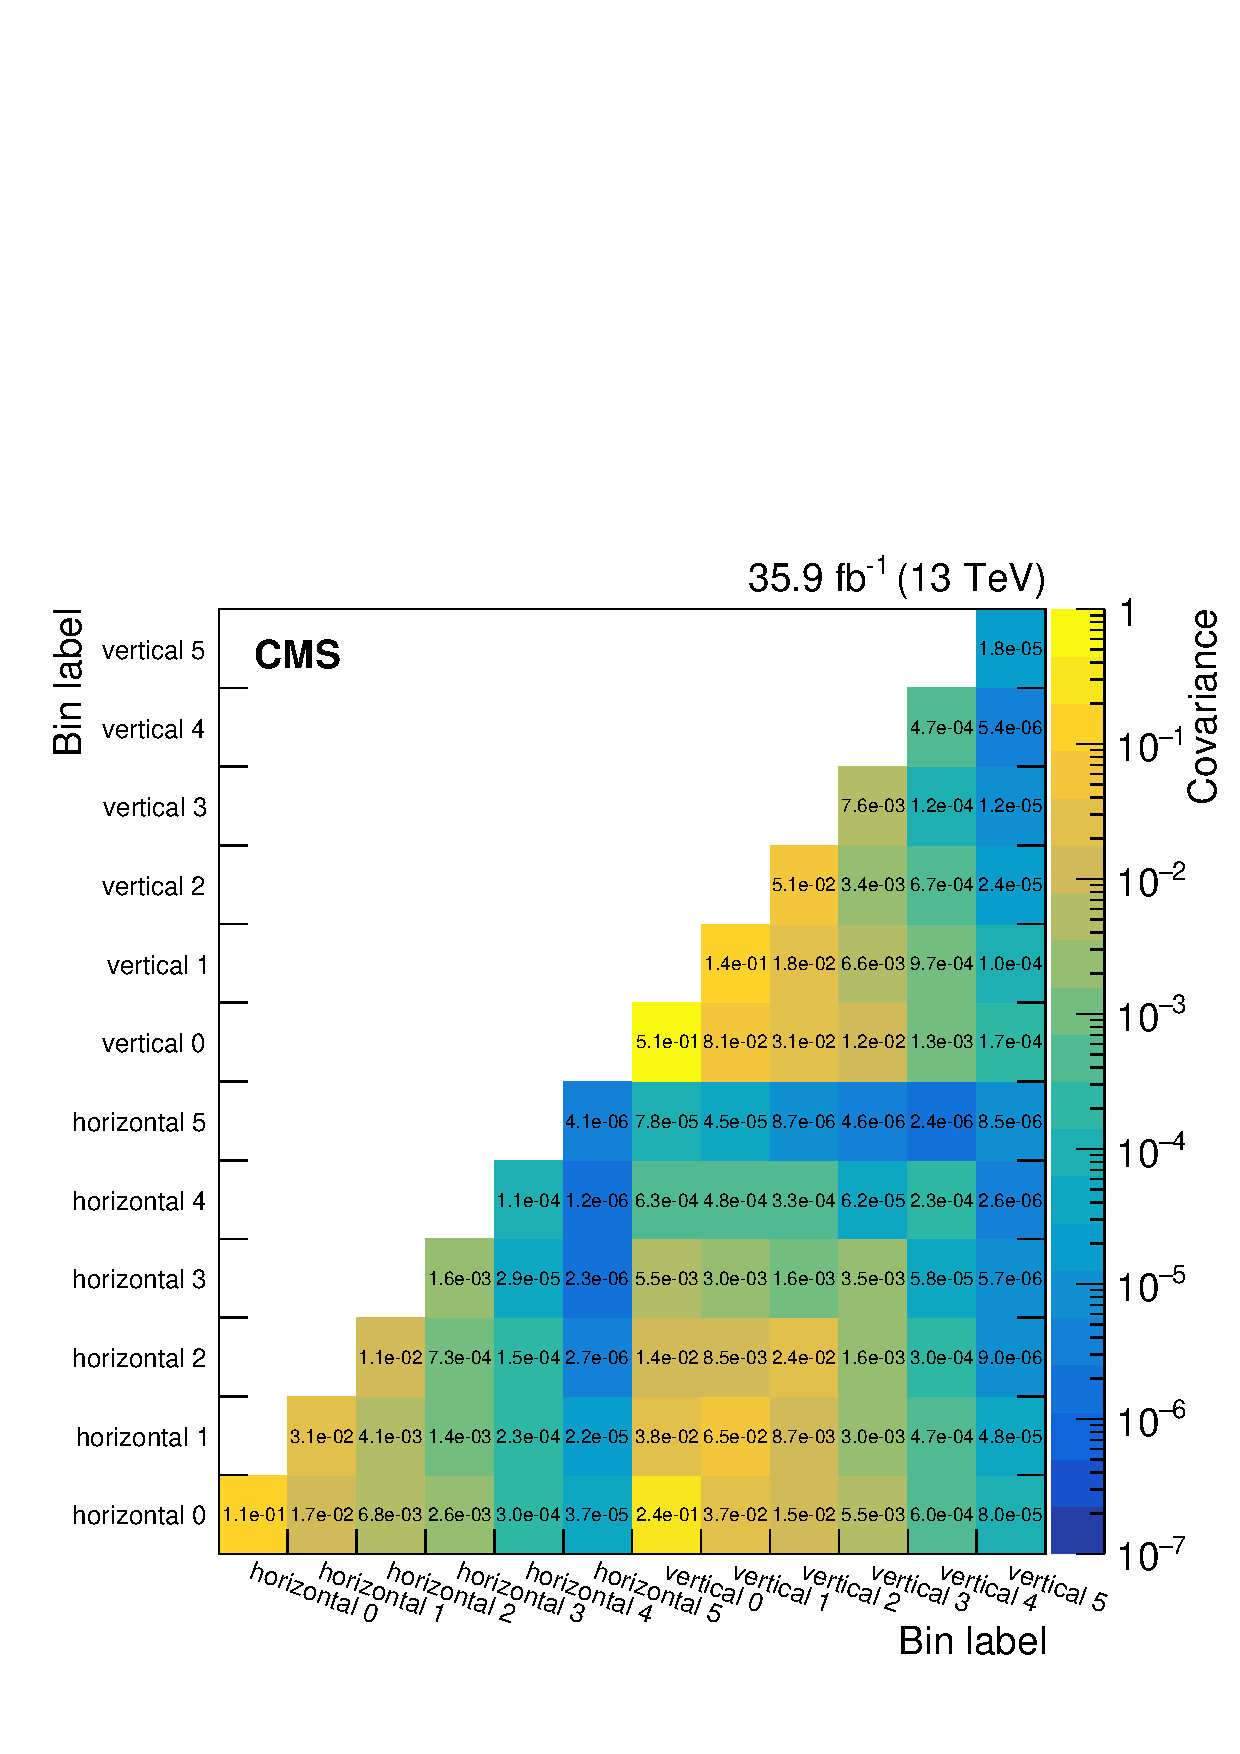
\includegraphics[width=0.9\textwidth]{Analysis/Figures/correlation_matrix.pdf}
  \caption{
    Covariances between the predicted background yields in all the \ETg\ bins of the horizontal and vertical signal regions.
    The bin labels specify which signal region the bin belongs to and what number bin it is for that region.}
  \label{fig:correlation_matrix}
\end{figure}.

\subsection{Limits}
\label{subsec:limits}

\begin{figure}[htbp]
  \centering
   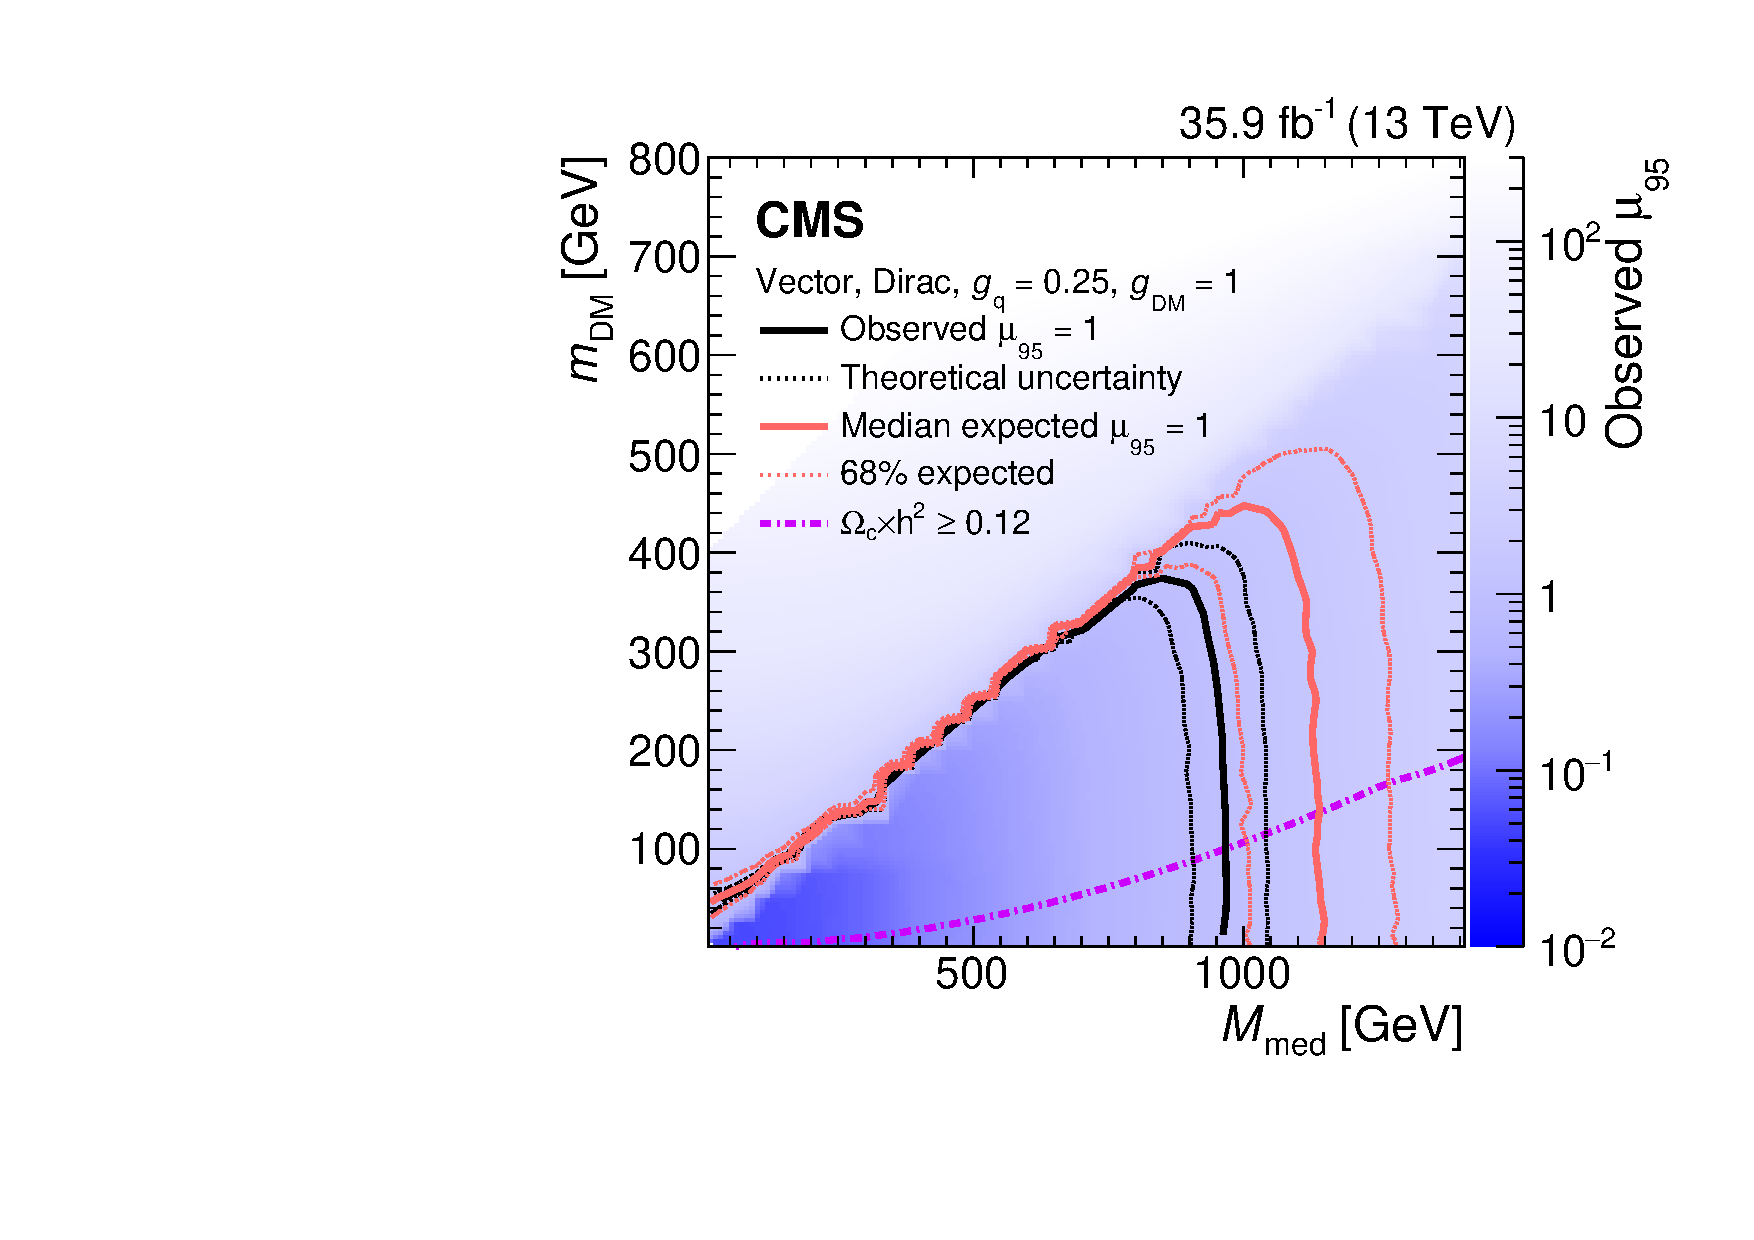
\includegraphics[width=0.48\linewidth]{Analysis/Figures/limits_vector.pdf}
    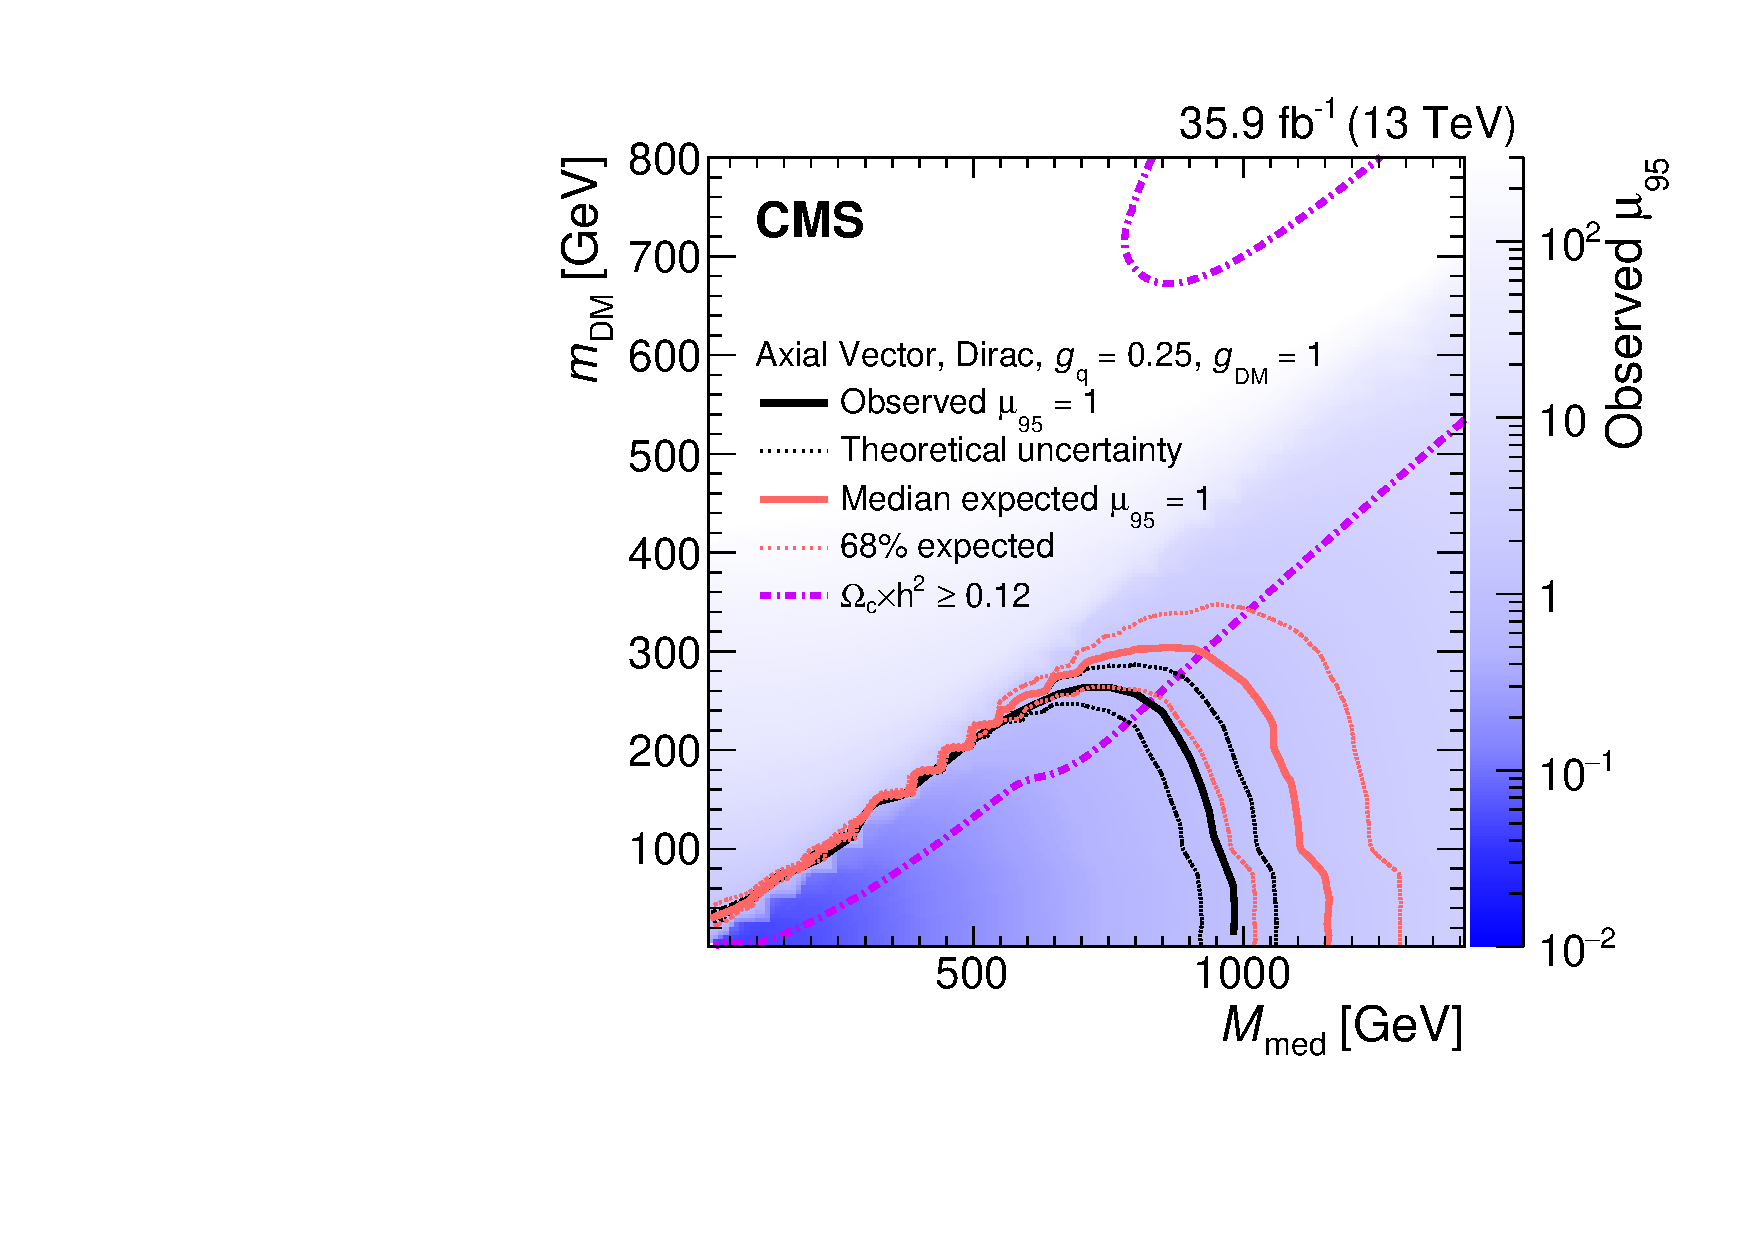
\includegraphics[width=0.48\linewidth]{Analysis/Figures/limits_axial.pdf}
    \caption{
      The ratio of 95\% \CL\ upper cross section limits to the theoretical cross section ($\mu_{95}$), for DM simplified models with vector (left) and axial-vector (right) mediators, assuming $\gq=0.25$ and $\gDM=1$.
      Expected $\mu_{95} = 1$ contours are overlaid in red. 
      The region under the observed contour is excluded. For DM simplified model parameters in the region below the lower violet dot--dash contour, and also above the corresponding upper contour in the right hand plot, cosmological DM abundance exceeds the density observed by the Planck satellite experiment.
    }
    \label{fig:limits}
\end{figure}

Figure~\ref{fig:limits} shows the 95\% \CL\ upper cross section limits with respect to the corresponding theoretical cross section ($\mu_{95}= \sigma_{95\%}/\sigma_{\text{theory}}$) for the  vector and axial-vector mediator scenarios, in the \mmed--\mdm\ plane. 
The solid black (dashed red) curves are the observed (expected) contours of $\mu_{95} = 1$. 
The $\sigma_{\text{theory}}$ hypothesis is excluded at 95\% \CL\ or above in the region with $\mu_{95} < 1$. 
The uncertainty in the expected upper limit includes the experimental uncertainties. 
For the simplified DM LO models considered, mediator masses up to 950\GeV are excluded for values of \mdm\ less than 1\GeV.

\chapter{Comparison with Other Results}

We're not doing this in a vacuum.

\section{Monophoton}

\section{Monojet / Mono-$Z$}

\section{Direct Detection}

The exclusion contours for the vector mediator model shown in Fig.~\ref{fig:limits} are also translated into the $\sigma_{\text{SI}}$--\mdm\ plane, where $\sigma_{\text{SI}}$ are the spin-independent DM--nucleon scattering cross sections as shown in Fig.~\ref{fig:limits_direct}. 
The translation and presentation of the result follows the prescription given in Ref.~\cite{Boveia:2016mrp}.
In particular, to enable a direct comparison with results from direct detection experiments, these limits are calculated at 90\% \CL~\cite{dmforum}.
When compared to the direct detection experiments, the limits obtained from this search provide stronger constraints for DM masses less than 2\GeV for spin independent models.

\begin{figure}[htbp]
  \centering
    \includegraphics[width=0.48\linewidth]{Impact/Figures/limits_direct.pdf}
    \caption{
      The 90\% \CL\ exclusion limits on the $\chi$--nucleon spin-independent scattering cross sections involving the vector operator as a function of the \mdm.
      Simplified model DM parameters of $\gq=0.25$ and $\gDM=1$ are assumed.
      The region to the upper left of the contour is excluded. 
      On the plots, the median expected 90\% \CL\ curve overlaps the observed 90\% \CL\ curve.
      Also shown are corresponding exclusion contours, where regions above the curves are excluded, from the recent results by the CDMSLite~\cite{Agnese:2015nto}, LUX~\cite{Akerib:2016vxi}, PandaX-II~\cite{Cui:2017}, XENON1T~\cite{Aprile:2018}, and CRESST-II~\cite{Angloher:2015ewa}.
    }
    \label{fig:limits_direct}
\end{figure}

\section{Indirect Detection}

The exclusion contours for the axial-vector mediator model shown in Fig.~\ref{fig:limits} are also translated into the $\sigma_{\text{SD}}$--\mdm\ plane, where $\sigma_{\text{SD}}$ are the spin-dependent DM--nucleon scattering cross sections as shown in Fig.~\ref{fig:limits_indirect}. 
The translation and presentation of the result follows the prescription given in Ref.~\cite{Boveia:2016mrp}.
In particular, to enable a direct comparison with results from indirect detection experiments, these limits are calculated at 90\% \CL~\cite{dmforum}.
When compared to the indirect detection experiments, the limits obtained from this search provide stronger constraints for DM masses less than 200\GeV for spin dependent models.

We show the results in Fig.~\ref{fig:limits_indirect}.

\begin{figure}[htbp]
  \centering
    \includegraphics[width=0.48\linewidth]{Impact/Figures/limits_indirect.pdf}
    \caption{
      The 90\% \CL\ exclusion limits on the $\chi$--nucleon spin-dependent scattering cross sections involving the axial-vector operator as a function of the \mdm.
      Simplified model DM parameters of $\gq=0.25$ and $\gDM=1$ are assumed.
      The region to the upper left of the contour is excluded. 
      On the plots, the median expected 90\% \CL\ curve overlaps the observed 90\% \CL\ curve.
      Also shown are corresponding exclusion contours, where regions above the curves are excluded, from the recent results by the PICO-60~\cite{Amole:2017dex}, IceCube~\cite{Aartsen:2016exj}, PICASSO~\cite{Behnke:2016lsk} and Super-Kamiokande~\cite{Choi:2015ara} Collaborations.
    }
    \label{fig:limits_indirect}
\end{figure}

% \chapter{Conclusion}
\label{sec:conclusion}

Things to conclude.

%% \appendix
%% \chapter{Tables}

\begin{table}
\caption{Armadillos}
\label{arm:table}
\begin{center}
\begin{tabular}{||l|l||}\hline
Armadillos & are \\\hline
our	   & friends \\\hline
\end{tabular}
\end{center}
\end{table}

\clearpage
\newpage

%% \chapter{Figures}

\vspace*{-3in}

\begin{figure}
\vspace{2.4in}
\caption{Armadillo slaying lawyer.}
\label{arm:fig1}
\end{figure}
\clearpage
\newpage

\begin{figure}
\vspace{2.4in}
\caption{Armadillo eradicating national debt.}
\label{arm:fig2}
\end{figure}
\clearpage
\newpage

%% This defines the bibliography file (main.bib) and the bibliography style.
%% If you want to create a bibliography file by hand, change the contents of
%% this file to a `thebibliography' environment.  For more information 
%% see section 4.3 of the LaTeX manual.
\begin{singlespace}
\bibliography{main}
\bibliographystyle{plain}
\end{singlespace}

\end{document}
